\documentclass[11pt,a4paper,twocolumn]{scrbook}
\usepackage[table,x11names]{xcolor}
\usepackage[utf8]{inputenc}
\usepackage{aurical}
\usepackage[l,nf]{coelacanth}
\usepackage[T1]{fontenc}
\usepackage[english]{babel}
\usepackage{enumitem}
\usepackage{longtable}
\usepackage{graphicx}
\usepackage{hyperref}
\usepackage{bookmark}
\usepackage{fullpage}
\usepackage{eso-pic}
\usepackage{incgraph,tikz}
\usepackage{mdframed}
\usepackage{subcaption}
\usepackage{caption}
\usepackage{nameref}
\usepackage{titleref}
\usepackage{float}
\usepackage{placeins}
\usepackage{pdflscape}
\usepackage{xfrac}
\usepackage{multicol}

\DeclareCaptionFont{blue}{\color{LightSteelBlue3}}

\hypersetup{pdftex,colorlinks=true,allcolors=blue}

\usetikzlibrary{positioning}

\newcommand\litem[1]{\item{\bfseries#1.\space}}

\definecolor{light-grey}{gray}{0.85}

\newcommand*\cleartoleftpage{%
  \clearpage
  \ifodd\value{page}\hbox{}\newpage\fi
}

% Notes for DM's
%
\newenvironment{note}{
  \begin{mdframed}[roundcorner = 5pt,
                   skipabove=0.3cm,
                   leftmargin=0.2cm,
                   rightmargin=0.2cm]
    \begin{centering}
      \textbf{\large{Notes for Dungeon Masters}}
    \end{centering}
    \par
}{
  \end{mdframed}
  \par
}

% That one song quote
%
\newcommand\songquote[2]{
  \begin{center}
    ``#2'' \\ - \emph{#1}
  \end{center}
}

% Environment for 3.5e rules
%
\newenvironment{35e}[1]{%
  \begin{mdframed}[roundcorner = 5pt,
                   skipabove=0.3cm,
                   leftmargin=0.2cm,
                   rightmargin=0.2cm]
    \begin{centering}
      \textbf{\large{#1 (3.5)}}
    \end{centering}
    \par
}{
  \end{mdframed}
  \par
}

\newcommand{\featref}[1]{%
  \hyperref[feat:#1]{#1}
}

\newenvironment{ebtable}[1]{%
  \begin{table*}[!htb]
    \captionsetup{labelformat=empty,font={large,bf},position=top}
    \caption{#1}
    \rowcolors{1}{white}{light-grey}
}{
  \end{table*}
}

%% The 3.5e materials have a style where they start with
%% with a bold face header text, following by a colon and
%% then the description text. \srditem{header}{description}
%% simulates exactly that.
%%
\newcommand{\srditem}[2]{%
  \par \noindent \textbf{#1}: #2
}

\newcommand{\srdbackgroundfeat}[0]{
  \srditem{Background Feat}{This feat is a background feat and reflects the
    environment, culture, and society you grew up in. It can only be taken at
    level 1, and does not count towards your maximum allowed feats of level
    1. But only one background feat may be taken at level 1, unless racial
    bonuses allow for additional background feats.}
}

%% Begin a new feat block. Multiple \srditem should be used to recreate
%% the look of the original 3.5e books
%%
\newenvironment{35efeat}[1]{
  \vspace*{0.3cm}
  \begin{centering}
    \textbf{\large{#1}}\label{feat:#1}
  \end{centering}
}{
  \par
}

%% Begin a new soul power block. Multiple \srditem should be used to recreate
%% the look of the original 3.5e books
%%
\newenvironment{soulpower}[1]{
  \vspace*{0.3cm}
  \begin{centering}
    \textbf{\large{#1}}\label{soulpower:#1}
  \end{centering}
}{
  \par
}

%% Common SRD things for spells
\newcommand{\level}[1]{\srditem{Power Level}{#1}}
\newcommand{\components}[1]{\srditem{Components}{#1}}
\newcommand{\castingtime}[1]{\srditem{Casting Time}{#1}}
\newcommand{\target}[1]{\srditem{Target}{#1}}
\newcommand{\range}[1]{\srditem{Range}{#1}}
\newcommand{\rangetouch}[0]{%
  \srditem{Range}{Touch}
  \srditem{Target}{Creature touched}
}
\newcommand{\rangepersonal}[0]{%
  \srditem{Range}{Personal}
  \srditem{Target}{You}
}
\newcommand{\rangeclose}[0]{\srditem{Range}{Close (25 ft. + 5 ft./2 levels)}}
\newcommand{\duration}[1]{\srditem{Duration}{#1}}
\newcommand{\instantaneous}[0]{\srditem{Duration}{Instantaneous}}
\newcommand{\savingthrow}[1]{\srditem{Saving Throw}{#1}}
\newcommand{\raising}[1]{\srditem{Can be raised}{#1}}


\newcommand\aren[1]{
  \begin{addmargin}[0.5cm]{0.5cm}
    ``#1'' - \emph{Aren Fel}\\
  \end{addmargin}
}

\newcommand\graham[1]{
  \begin{addmargin}[0.5cm]{0.5cm}
    ``#1'' - \emph{Graham Balance}\\
  \end{addmargin}
}

\title{Everblack:\linebreak Wayfaerer's Guide to Aror}
\author{
  Archmagi Graham Balance\\
  \and
  Aren Fel
}
\date{Original version by Archmagi Graham Balance in GT:2104\\
  Continous updates ever since then, by Aren Fel
}

\unsettoc{toc}{onecolumn}

\begin{document}

\setcounter{secnumdepth}{0} % sections are level 1

\maketitle

% Put world map right here, after the title, making them the
% second and third page
\cleartoleftpage

\incgraph{media/worldmap-a3-left.png}

\clearpage

\incgraph{media/worldmap-a3-right.png}

\clearpage


% Credits
\onecolumn

\songquote{In Flames}{
  Hypnagonia's lucid horizons\\
  Play with the yearning I have quelled\\
  As I strike towards the pantheon\\
  And what therein is held
}

\vspace*{\fill}

\begin{center}
  Get the latest version of the PDF at <\href{https://aror.org}{aror.org}>

  \textbf{Author}\\
  Florian Stinglmayr
  <\href{mailto:fstinglmayr@gmail.com}{fstinglmayr@gmail.com}>

  \textbf{Artwork}\\
  Asya Yordanova
  <\href{https://artstation.com/asya\_yordanova}{artstation.com/asya\_yordanova}> \\
  Paula Wiśniewska
  <\href{http://aianeart.com}{aianeart.com}>

  \textbf{Special Thanks:}\\
  Philipp ``muddasheep'' Lehner\\
  Raul Fuentes
\end{center}

\twocolumn
\newpage


% Two column table of contents
\tableofcontents
\newpage

% Enable two columns mode for everything, undo this in specific
% chapters later where it makes sense.
\twocolumn

% Chapter 1: Introduction
\chapter{Everblack Campaign Setting}

The \emph{Everblack} campaign setting is a D\&D setting for 3.5e.  It is
written from the view of the two most prominent NPCs of the world:
\emph{Graham Balance} an influential archmagi and bard, and \emph{Aren Fel},
also known as the \emph{Undying Witch}, a chronicler and priestess of the
\emph{Silent Queen}. But more about them later on.

It is in fact a labour of love of one person, with input from many different
people and players. It was started in 2015 and continuously enhanced and
refined the course of many years.

\section{Tone of Everblack}

One of the main defining features of \emph{Everblack} is the tone and attitude
of the campaign setting. It combines traditional fantasy settings with the love
for horror and a more EU centric lore. It also aims to introduce grit, moral
ambiguity, shades of moral gray and an everlasting fear of
death. Although \emph{Dark Sun} already does many of these aspects extra
ordinarily well already, \emph{Everblack} does not rely on a
post-apocalyptic surrounding. It's just that in \emph{Everblack} everything
tries to eat, kill or enslave you while you can also sniff pretty flowers on
the side of the road. However this does not mean that good does not exist in
this world. Like spices in cooking, you can overdo gritty and dark concepts in
a work of fiction.

The world of \emph{Everblack} is old, and rich in history. Filled with old
legends, gods long dead, and civilisations that have long fallen. Those that
venture outside the save walls of the major city kingdoms, will find strange
creatures, obscure cults, death and peril, but also adventures, powerful
artefacts and great riches.

Magic is a major part of the setting, and is augmented by a new, and fourth
form of magic: \emph{soul magic}. While in \emph{Everblack} both arcane and
divine magic come from the gods, \emph{soul magic} is inherent to every living
being, much like psionic powers. However \emph{soul magic} is often
misunderstood, shunned and even forbidden by the followers of the lesser gods.

But still the world of \emph{Everblack} is a place where adventurers set forth
to slay the beast and bring back the gold. A world full of magic, ancient
artifacts, but also of eldritch horrors, great strife and despair.

\section{Seven things to you should know}

\begin{enumerate}
 \litem{Not everything within D\&D fits} Many creatures, concepts, classes and
 races that are part of the basic D\&D do not fit into \emph{Everblack}. Some
 monsters may be extinct, classes might be rarer in \emph{Everblack} than
 elsewhere, and some concepts do not directly fit within the world
 itself. While this might bar you from certain concepts and mechanics, this
 was done deliberately to enhance the tone and attitude of the campaign
 setting.

 \litem{Overall tone} \emph{Everblack} attempts to blend horror and evil with
 D\&D. It aims to convey a world where ancient malevolent beings rule from the
 shadows. Where horrible and sadistic creatures just lurk in the dark forest
 beyond your village waiting for the perfect opportunity to strike. Where the
 world itself is dark, horrible, cruel, unfair, dirty and filthy. A world were
 slavery is as much accepted, as an evil Inquisition that enacts vigilante
 justice across the face of the world. Where evil witches are meticulously
 persecuted and burnt at stake, and entire city kingdoms move forth with a
 continent wide genocide of what they deem \emph{lesser} races.
 \emph{Everblack} is not a nice neighbourhood.

 \litem{Soul Magic} The setting introduces a new, fourth kind of magic to the
 world: \emph{soul magic}. It postulates that every living being has a soul,
 from which the being can draw power from. This power might enhance martial
 abilities or may be directly shaped into magic spells. Arcane and divine
 magic comes directly from the realm of the gods, and they have used both as a
 tool to manipulate the mortal races for aeons. Often
 \hyperref[sec:Religion]{lesser deities} see soul magic as an aberration, and
 thus manipulate their followers into seeking out and destroying soul magic
 everywhere they can find it. To those untrained in the arts of the soul, a
 soul afflicted person might just another undead creature, fuelling
 misconceptions and ignorance among the general populace.

 \litem{Aror is a global place} The planet of Everblack, known as Aror, has a
 few very important and big city kingdoms which are connected with each other
 with an arcane teleporter network. Although the cities charge money for the
 usage of these teleporters it has made the world smaller. Commoners, traders
 and adventurers use them regularly to visit other city kingdoms, to travel,
 do trade and exchange cultures. These teleporters are limited to large cities
 as the network requires constant care of magi and wizards to be kept
 operational.

 \litem{Everblack} The setting is named after the \nameref{sec:Everblack}
 crystal. Pitch black crystals that can store any magical energy. They are
 often used to aid casters, fuel arcane machinery. \emph{Everblack} is
 extremely rare, so much so that shards of it have replaced platin as the
 major currency for large purchases. The crystals are used in \emph{soul
 magic} research, but also in arcane experiments and arcane machinery. It his
 highly sought after all across the world, and entire societies depend on it
 for mining, trade and arcane constructions.

 \litem{New Races} In addition to the common player races, \emph{Everblack}
 introduces three new races: the \nameref{sec:Deepkin}, \nameref{sec:Diarim}
 as well as the \nameref{sec:Umgeher}. Deepkin are the cavern dwelling cousins
 of the human races, with dark vision, bright white skin and flowing red
 hair. While Umgeher are a half undead species of humans that were created by
 powerful vampires a long time ago as servants. Diarim are an slave race which
 were bred by the giants for battle against their mortal enemies the dragons.

 \litem{Death means Death} unlike many other settings death is often final
 within the world of Everblack. Only the gods themselves can raise people from
 the dead by first transporting their souls to their realm. If a god lifts you
 to their realm, and then releases you again is within their own power to
 decide. Although the divine magic for raising dead is available, it fails more
 often than it succeeds. The gods rarely release their new possessions, soul
 included. But this fear of death holds true for everyone. An outsider is not
 sent back to his or her home plane on death, but dies. Permanently. Fey are
 not mysteriously birthed again in the world should they die or be slain, no,
 they die forever just like the rest of the mortal souls on the world.

\end{enumerate}

\pagebreak

\onecolumn
\section{Foreword by Graham Balance}

The following book should serve you well as an introduction to the
place you might only know as the place \emph{where everblack comes
  from}. I, Archmagi Graham Balance, would like you welcome you to
our corner of the multiverse: ``Aror''.

This book will serve you as a guide to Aror's many places, cultures,
customs, people and creatures. I am fortunate to have counted this
place as my home for many years, and it holds a special place in my
heart. Great was the dismay when I had to discover on my frequent
travels and journyes to other planes, that our tiny little speck of
the multiverse was not very well know, or perhaps only known as the
``place where Everblack crystals come from''. While true, it saddens
me deeply to see our fine planet, and its people, reduced to the mere
fact that we export black crystals charged with arcane energy. That
experience was the sole motivator on why I am wrote this book: To bring
our way of life to you, dear reader.

I have interviewed many that did come to Aror, and most of them only
remembered the bad things that had happened to them in their short
visit: unfriendly locals speaking weird tongues, stale ale, and the
occasional blind subterranean humanoid that tried to eat them. While
many of these aspects are true, they are warped exaggerations of the
truth. My sincere hopes are that, after reading through this book, you
have arrived at the conclusion that Aror is a place worth visiting,
that our ale is as good as any - if not better - and that the
cannibalistic blind humanoid creatures of the deep are too far and few
between to be a real threat.

You will have heard our most treasured places, such as the holy lake
of \emph{Mu'ut} in the south; the lone yet towering \emph{Goban}
mountain in the east; the endless treasures, archipelagos and beaches
that the \emph{Silver Isles} have to offer; or the vast mountains,
lush forests, and friendly locals of \emph{Eilean Mor}. If that does
not impress you, I am sure the grandious library and arcane college of
\emph{Fes el-Bali}, the towering cliff side castle of \emph{Forsby} or
the endless riches in art and music of \emph{Nen-Hilith} surely will
make a lasting impression.

\section{Additional Foreword by Aren Fel}

My good old friend Graham is right in one aspect: Aror has an insidious
way of sneaking into your heart, embedding itself so deeply that not
even a Dryad could convince the roots to leave you. But he is wrong in
so many other things. The ale has not gotten better, and the people
are still unfriendly. But much has changed since the almost 4000 years
this book was originally published. Gods have vanished, civilisations
have fallen, generations have been born and have died; and most important
of all - cultures, languages and entire epochs have been lost only to be
rediscovered centuries later.

I, Aren Fel, have done my best to adapt, change and translate the
book, so that the work of my good friend continues as he originally
intended: as an useful guide to our world, both past and present. In
many ways the book has now exceeded it's original purpose. It was once
a mere introduction to Aror, but it is now also a chronicle of our
history. A lens into our past, and perhaps a warning for our future.

Be safe adventurer, and fasten this book to your belt for easy access,
in case any blind cannibalistic humanoids chase you throw a cavern.
\twocolumn


% Chapter 2: Races
\chapter{Races}
\label{sec:Races}

\section{Introduction}

The people of Aror make up a multi flavoured stew of various races and
backgrounds. Apart from many races that you might be already familiar with,
such as humans, elves, dwarves or gnomes; Aror is also home to some you might
have never heard of before. Some of these are the
\hyperref[sec:Deepkin]{deepkin}, the \hyperref[sec:Diarim]{diarim},
\hyperref[sec:Gorgons]{gorgons} and the \hyperref[sec:Umgeher]{umgeher}.

You will find that race matters little. An elf of \nameref{sec:Norbury} often
shares the warrior culture, and faith in the meritocratic societal ideas
of Norbury much like any human or halfling living there. While a dwarf of
\nameref{sec:Nen-Hilith} will be accustomed and to the artistic culture and
creative ways of the artisans and performers of that city.

The union of non-humanoid races with humanoid races is something that does not
exist in \emph{Aror}. Although you might have met ``dragonborn'' (the unity of
a human and a dragon) in other realms, you will not find them on Aror. And if
you do, they are probably extra-planar visitors much like yourself.

\begin{note}
  These sections enhance or change the existing core races of D\&D. Any lore
  you find in the base books that does not interfere with what is written
  here, still holds true.
\end{note}

\section{Core Races}
\label{sec:Core Races}

\ifimages
\begin{figure*}[ht!]
    \centering
    \vspace{-2.6cm}
    \centerline{
      \includegraphics[width=\paperwidth,keepaspectratio]{%
        media/coreracessm.\imagesuffix
      }
    }
    \par
    Core humanoid races of Aror: humans, elves, dwarves and halflings.
\end{figure*}
\fi

The core humanoid races of Aror are those races that originate from the
original dwarves, humans, halflings and elves that left the content of
\nameref{sec:Arania} thousands of years ago. Deepkin and Humans are listed as
separate species, yet they are very close to one another. Even though some
species have shown variants, such as elves and humans, all of these are still
close enough to one another to produce viable offspring in an union.

The core races generally have good relations with one another, and also live
happily together in large city kingdoms, baronies or towns. The only exception
being a few secluded, traditionalist and xenophobic dwarven clans that prefer
to isolate themselves into their mountains. But their open minded,
good-spirited, and city dwelling cousins outnumber them easily a hundred times
over.

\subsection{Deepkin}
\label{sec:Deepkin}

\aren{I had the misfortune of seeing my people's decline with my own eyes.
I was powerless, and unable to stop it. We are but a shadow of our former
selves...}

\graham{But still you live. And once the time is right, you may reclaim what
once was.}

The \emph{deepkin} are the cavern dwelling cousins of humans. They are capable
of seeing in the dark (albeit without perceiving colour), and often have white
pale skin, red to brownish hair, and either red, green, blue or yellow eyes.

Deepkin society is one of the older societies on \emph{Aror}, with a long
standing history in the arcane arts, building magnificent underground cities,
libraries and workshops. Ancient deepkin were master arcane smiths, golem
constructors, inventor of many magic based constructs and technology still
used today.

The ancient deepkin had their dominance challenged by the other races of the
deep, namely the dwarves, dark elves, and a now almost extinct species called
the \nameref{sec:Ilians}. Hundreds of years of conflicts lead to the decline
of most of their impressive civilisations, with one exception. Instead of
perishing however, most of them fled to the surface, where they were warmly
received by their surface cousins. Nowadays deepkin culture is but a shadow of
what it was, although they still try to reclaim what was once theirs with
expeditions into the deep. Albeit they were well known city and kingdom
builders, only one deepkin settlement rose to the rank of a formidable city
kingdom: \emph{Stenheim}.

Although deepkin are treated as their own race, they are still capable of
producing viable offspring with normal humans. The race of the offspring is
always that of the mother, due to the dominant genetic traits of the deepkin.

\begin{35e}{Deepkin Traits}
  \hyperref[sec:Speak Language]{Doresh} is the natural language of the
  Deepkin, and is equivalent to \emph{Undercommon}.

  \begin{itemize}[noitemsep]
    \item Medium: as medium creatures, \emph{Deepkin} have no special bonuses or
    penalties due to their size.
    \item \emph{Deepkin} base land speed is 30 ft.
    \item For all manners regarding racial restrictions or classifications
    \emph{Deepkin} count as humans.
    \item Dark vision out to 120 feet.
    \item Bonus Feat: Just as their human cousins, \emph{Deepkin} can choose a
    bonus feat at first level.
    \item Automatic languages: Doresh, Teranim. Bonus Languages: Any (except
      secret languages)
    \item Favoured Class: Any. When determining whether a multi class takes an
    experience point penalty, his or her highest-level class does not count.
  \end{itemize}
\end{35e}

\subsection{Dwarves}
\label{sec:Dwarves}

\emph{Dwarves} are a race of short humanoid species, belonging to four core
races that left \nameref{sec:Arania} several millennia ago. By nature dwarven
are smaller than the other races. Their stout physique lends them to tasks that
require prolonged endurance, and are thus natural labourers, and warriors.
Much like their closely related core humanoid cousins, most dwarves enjoy
living with the other core humanoid races in large kingdoms, cities, and
towns.

The dwarves that still remain in the depths are often not as open, welcoming
and tolerant. These dwarven tribes have survived the harsh realities of the
deep by creating a strictly ordered society based on castes. The clans of the
deep might be slow to trust foreigners, reclusive, isolationists, or outright
xenophobic. This culture a foundation of the the kingdom of
\nameref{sec:Kesmar}, which was founded by an isolationist, and xenophobic
tribe of dwarves millennia ago. Such dwarven cultures are only a fraction of
the living dwarven population however, and the vast majority of them live
happily together with their brethren.

\begin{35e}{Dwarf Traits}
  \emph{Rutari} is the language that dwarves of the deep speak, and is also
  the language of \nameref{sec:Kesmar}. It has its own alphabet, which is
  also called Rutari.

  \begin{itemize}[noitemsep]
    \item Medium: As Medium creatures, dwarves have no special bonuses or
      penalties due to their size.
    \item Dwarf base land speed is 20 feet. However, dwarves can move at this
      speed even when wearing medium or heavy armor or when carrying a medium or
      heavy load (unlike other creatures, whose speed is reduced in such
      situations).
    \item Dwarves are sturdy and hardy, and thus have a +2 racial bonus to
      constitution.
    \item Stability: A dwarf gains a +4 bonus on ability checks made to resist
      being bull rushed or tripped when standing on the ground (but not when
      climbing, flying, riding, or otherwise not standing firmly on the
      ground).
    \item Languages: Rutari, Teranim. Bonus Languages: Any (except secret
      languages)
    \item Favoured Class: Any. When determining whether a multi class takes an
          experience point penalty, his or her highest-level class does not
          count.
  \end{itemize}
\end{35e}

\subsection{Elves}
\label{sec:Elves}

Elves are tall - often between 1.8 and 2.4 metres - and slender race, with
long and pointy ears. The style of the elven ears varies, with some having
smaller pointy ears facing backwards, while others have longer and sharper
ears that follows the contours of their face. The variety within the elven
ears is vast, but is but a minor cosmetic difference. Their physique and build
is slender as well, with long skinny legs and arms. Elves live up to 400 years
of age, and thus often pick up professions that take longer to master, such as
wizardry, artistry or the sciences. Although elves live long, they often shift
focus in their goals. Apart from the humans, the elves are one of the older
races of \emph{Aror}.

Unlike humans, elves do have distinct sub races that differ from each other in
various physical and biological aspects. The \emph{snow elves} for example
have a natural resistance to cold like no other species have, while the
\emph{dark elves} have adapted to see better in the dark caverns they
inhabit. However they have not diverged so far from one another to not produce
vialable offspring. As with humans and deepkin the race of the sibling always
resembles that of the mother.

There are four major elven races that are recognised across the world of
\emph{Everblack}:

\subsubsection{High Elves}
\label{sec:High Elves}

The most numerous race of the elves are the \emph{high elves} of
\nameref{sec:Avenfjord}. High elves have fair skin with a hint of yellow and
gold. Their hair ranges from blond, fiery red to brown and black. They stand
between 1.8 and 2.4 metres high, towering with their slender appearance over
most other humanoid races with ease. They have pointed, elongated ears which
often point skyward, following the slender contour of their face.

High elves are the most adaptable and curious of the elves, and often live
within human city kingdoms, mixing and integrating well with other cultures
and societies. Even though they have their own kingdom, the vast majority of
high elves live outside the kingdom of Avenfjord. High elves are the only
kingdom building elven race, but do prefer to live with together with their
distant human cousins within baronies, kingdoms and city states.

The high elves are also the longest living of all the elven races, usually
living to grow 400 years old. This gives them ample time to study and learn
several fields and areas of expertise during their early childhood.

High Elves speak \hyperref[sec:Speak Language]{Enro'ad}, a variant of
\emph{Old Teranim}, but use the Taavid, halfling alphabet called \emph{Taavid}
to write it.

\begin{35e}{High Elf Traits}
  \hyperref[sec:Speak Language]{Enro'ad} is elvish, albeit the elven alphabet
  is now written with Taavid the \emph{halfling} script.

  \begin{itemize}[noitemsep]
    \item Medium: As Medium creatures, elves have no special bonuses or
    penalties due to their size.
    \item Low-Light Vision: An elf see twice as far as a human in starlight,
    moonlight, torchlight, and similar conditions of poor illumination. She
    retains the ability to distinguish colour and detail under these
    conditions.
    \item Elvish adulthood lasts longer than in other species, and they thus
      have more time to learn while they grow up. This grants them a +2 bonus
      to intelligence, and elves can select one extra
      \hyperref[sec:Education Feats]{education feat} at level 1.
    \item Automatic languages: Enro'ad, Teranim. Bonus Languages: Any (except
      secret languages)
    \item Favoured Class: Any. When determining whether a multi class takes an
    experience point penalty, his or her highest-level class does not count.
  \end{itemize}
\end{35e}

\subsubsection{Dark Elves}
\label{sec:Dark Elves}

The \emph{dark elves} live mostly underground, have black to blue skin, and
their hair ranges from a faint hint of blue, silver to snow white. Their eyes
are often red, blue or a green. They are the smallest of all elven races, and
range from 1.60 to 1.90 metres in height. In terms of bodily physique they
also more closely resemble humans. Their rounder faces, and their stronger and
more muscular physique sets them apart from their slender high elven cousins.

Dark elves once followed the dwarves underground, when the ancient battles
against the sentient non-humanoid creatures and the fey turned deadly and
dangerous. They have since adapted to that life underground, both physically
and culturally. They can see well in the dark, and their skin turned dark
letting them blend in with the dark surroundings of the depths. They also only
live roughly 120 years, and are thus not as long lived as their high elven
cousins.

Underground they are often live primitive, nomadic lives, adapted to the harsh
realities of the depths below. They have survived the dangerous environment of
the deep caverns by remaining on the move or by hiding from threats. They
value their small communities and family above all else.

Many dark elves also live on the surface, and much like their surface cousins,
they prefer to integrate into already existing humanoid kingdoms and baronies.
Dark elves are rather common all over the world, and can be found on almost all
continents.

\begin{35e}{Dark Elf Traits}
  \textbf{Dark Elf Traits (Ex)}: The following traits are in \emph{addition}
  to the high elf traits, except when noted.
  \begin{itemize}[noitemsep]
    \item Dark elves are considered smaller and more nimble than the other
      elven races, and thus gain a +2 racial bonus to dexterity.
    \item Dark vision out to 120 feet, albeit they are colour blind.
    \item Automatic languages: Doresh, Enro'ad, Teranim. Bonus Languages: Any
      (except secret languages)
  \end{itemize}
\end{35e}

\subsubsection{Snow Elves}
\label{sec:Snow Elves}

\aren{Snow Elves are the pinnacle of beauty...}

Far to the north and south live the \emph{snow elves}, nomadic hunter-gatherer
elves with white to silver blue skin, white, silver, grey or blue hair. Their
eyes are often bright blue, green or yellow. Male snow elves are capable of
growing facial hair, while many female snow elves have light red freckles
in their faces. Snow elves are as tall as their high elven brethren, ranging
from 1.8 to 2.4 metres, and also share most of their facial features with high
elves. They have adapted well to the colder climates, and can withstand the
cold far easier than any other humanoid race. This has also come with a major
drawback: With a life expectancy of 80 years, they are the elven race with
shortest lifespan. Many \emph{snow elves} live in smaller families and tribes,
content with surviving the harsh realities of the polar north and south by
becoming fierce hunters, fishers or even raiders themselves.

These snow elves from northern and southern tribes are generally known to be
calm, and quiet, preferring the solitude of a small group or town over the
vast masses and stretches of cities. They rarely leave the frozen north and
south, and are thus exotic, as in, many other humanoids haven't seen a tribal
snow elf in person. They do not build cities or kingdoms, but smaller tribes
often join to form larger ones (several hundred individuals) if required.

To tribal snow elves the community, family and their own tribe is everything, as
it ensures survival and in the frozen tundras. The harshest punishment within
these communities, reserved for major crimes, is exile which is often equal to
a death penalty. Since these exiles are then also shunned by other snow elven
tribes, they sometimes wander away from their homes and join city kingdoms or
baronies.

Snow elves rarely leave their icy domain and tribal lives willingly, and thus
the ancestors of the snow elves in the city kingdoms were either exiles, or
were once captured and brought there as slaves. Those civilised snow elves do
not harbour any animosity any more about what happened to their ancestors
thousands of years ago, and prefer to remain in the places and cultures they
now call their homes. To the tribal snow elves these city snow elves are equal
to exiles, and are thus not welcome in the frozen north or south.

\begin{35e}{Snow Elf Traits}
  \textbf{Snow Elf Traits (Ex)}: The following traits are in \emph{addition}
  to the high elf traits, except when noted.
  \begin{itemize}[noitemsep]
    \item \textbf{Pale Wastes (Su)}: A pale elf can live comfortably in
      conditions of extreme cold, even with barely any clothing or external
      sources of warmth. This ability functions like a continuous \emph{Endure
      Elements} but for cold conditions only.
    \item Snow elves are known for their great hunting skill which allows them
      to perceive hidden things and small details, and thus have a +2 bonus to
      wisdom.
    \item Automatic languages: Enro'ad, Teranim. Bonus Languages: Any (except
      secret languages)
  \end{itemize}
\end{35e}

\subsubsection{Wood Elves}
\label{sec:Wood Elves}

Wood elves have light brown or greenish skin, and green or red hair. Their
faces are often covered in light or red freckles, and their eyes are often
brown, blue or green. They are as tall as their high elven counter parts,
often ranging from 1.9 to 2.4 metres, and also share the facial features of
the other high elves. Although they are very close to their high elven
cousins, they are counted as their own race based on their ability to easily
build muscle mass. This often makes them the strongest elven race, and a wood
elf can easily be compared to \nameref{sec:Half-Orcs} in terms of bodily
strength. Even though they are known to join the major city kingdoms, they are
rarer than high or dark elves.

There are two major communities of wood elves. The first lives in the vast
temperate and boreal forest of \nameref{sec:Eilean Mor}, known as the
\nameref{sec:Dirgewood}. These wood elves live together with humans, halflings
of the Dirgewood, as well as the dark elves, deepkin and the dwarves of the
\nameref{sec:Great Divide}. They are followers of the \nameref{sec:Old Ways},
and prefer to build small settlements, towns and perhaps tiny cities of their
own. These wood elves are expert trackers, hunters, farmers, as well as shamans
and priests of the old ways.

And in the jungles \nameref{sec:Yuacata} live the \emph{savage elves}, a loose
collection of tribes of cannibalistic and demon worshipping wood elves. They
rarely wander beyond the confines of their jungle and are one of the rarest
elven culture to meet in the civilised areas of \emph{Aror}. They live a
primitive life, adapted to the harsh and dangerous rain forest.

\begin{35e}{Woold Elf Traits}
  \textbf{Wood Elf Traits (Ex)}: The following traits are in \emph{addition}
  to the high elf traits, except when noted.
  \begin{itemize}[noitemsep]
    \item Wood elves have it easier to gain muscle mass than the other elvish
      races, and thus have a +2 racial bonus to strength.
    \item Automatic languages: Enro'ad. Bonus Languages: Any (except secret
      languages)
  \end{itemize}
\end{35e}

\input{chapters/races/halflings}
\subsection{Humans}
\label{sec:Humans}

\emph{Humans} are one of the most prolific of the humanoid races of Aror, and
also the dominant race of the planet. Human artefacts have been found dating
back thousands of of years, outmatching the other humanoid races. There are
two separate ``races'' of humans: those inhabiting the southern part of the
hemisphere who usually have darker skin, and the ``northerners'' who usually
have fair skin. This distinction is superficial only. Apart from the tone in
skin colour, there is no other biological difference between the various human
tribes and civilisations. Humans live up to 80 years, and are known for being
statesmen, diplomats, farmers, adventurers, explorers and scientists.

Humans can be found everywhere on Aror. But history indicates that they
originated on the southern continent of \nameref{sec:Arania} together with the
other core humanoid races, and migrated to all other continents during the
last ice age twenty thousand years ago. Wherever humans settle they build
villages, cities, and large kingdoms and often become the dominant culture and
social structure. Human kingdoms have often endured for hundreds of years, and
have bested many difficulties that had driven other societies to ruin. The
ingenuity of the humans, their stubborn attitude and their uncanny ability to
adapt to any difficulty makes them the dominant race of Aror.

Like most races, humans have no inherent global culture, tradition or customs.
Instead their believes and customs are ever evolving, and specific to the
realm they live in. But there is one trait that the average human has: ingenuity
in the face of adversity. No other species has managed to settle every corner
of the world and endure, and even build lasting civilisations out of the
hostile environment they found themselves in.

\begin{35e}{Human Traits}
  \begin{itemize}[noitemsep]
  \item Medium: As Medium creatures, humans have no special bonuses or
    penalties due to their size.
  \item Human base land speed is 30 feet.
  \item 1 extra feat at 1st level.
  \item 4 extra skill points at 1st level and 1 extra skill point at each
    additional level.
  \item Automatic Language: Teranim. Bonus Languages: Any (other than secret
    languages).
  \item Favoured Class: Any. When determining whether a multiclass human takes
    an experience point penalty, his or her highest-level class does not count.
  \end{itemize}
\end{35e}

\subsection{Vampires}
\label{sec:Vampires}

Vampires are undead that were once humanoid creatures such as elves and
humans, that now mostly coexist peacefully with their mortal brethren.

There are two main types of vampires: those that drink \nameref{sec:Ramesk} or
monstrous blood and thus retain their mortal knowledge and character (called
``civilised vampires''), and those that have fallen for humanoid blood and
have turned feral (``feral vampires''). Both types of vampires retain their
physical appearance from when they were mortal (such as skin colour or body
shape and proportions), but gain retractable, elongated fangs as well as
retractable hardened finger nails that can act as claws.

A feral vampire's iris turn white (blinding them), and looses all abilities to
grow hair, or repair brittle or wounded skin, giving them a horrible, feral
and animal-like appearance compared to civilised vampires. Those vampires that
consume Ramesk regain their ability to see (their iris' are red), grow blue
hair and blue nails (which take the pigment from the blue Ramesk). But most
importantly the Ramesk allows them to suppress the hunger for blood, freeing
their minds and souls to follow other thoughts and feelings, without having an
obsessive and oppressive urge to seek out their next meal. Feral vampires' skin
is damaged by direct exposure to the suns, and they will avoid it if possible.
Although the skin of a civilised vampire is also damaged by the suns, the
effect is less severe, and many civilised vampires walk around during the day
by covering their skin with clothing.

Civilised vampires can fall feral if they begin feasting on humanoid blood,
and likewise feral vampires can return to a civilised behaviour with the help
of monstrous blood or Ramesk. This process is not instantaneous, but takes
place over the course of weeks. So even a civilised vampire may drink humanoid
blood once or twice without experiencing immediate deterioration.

Vampires are under direct threat by many militant religious organisations such
as the knights of \nameref{sec:Lor} or the \nameref{sec:Nightwatch}, but have
their own part of a kingdom in \nameref{sec:Helmarnock} where they might live
in peace together with other humanoids and vampires.

\subsubsection{History}

During the \nameref{sec:Aeon of Strife} many humanoid clans prayed to what
they believed was the greater deity \nameref{sec:Morana}. She in turn revealed
to her followers a path to great power to vanquish their foes, and many of her
followers accepted it. They were betrayed by their goddess and turned into
vampires.

These followers were turned undead, enhanced with special abilities, and were
given an insatiable hunger for monstrous blood. The vampires' hunger for
monstrous blood grew with every taste of the crimson liquid, perpetuating a
cycle of hunting, killing and feasting to satiate their thirst. Most humanoid
tribes that had people turned into vampires began locking themselves away at
night while allowing the vampires to roam the surrounding forests and area to
feast on those monstrous creatures unfortunate enough to remain outdoors
during the night. While in some areas the vampires spread terror and death
among the monstrous creatures that would attack the humanoid settlements, in
others, the lack of alternate food sources forced the vampires to turn on
those they were supposed to protect. These vampires then learned of yet
another betrayal by their mother: Vampires that feasted on the blood of the
core humanoid races (human, elf, dwarven, halfling and half-breeds) blood
would turn feral, and lose the last remaining modicum of control they had left
over their inner hunger. This lead them to be ostracised, hunted, and even
killed by their own people, the humanoids they were supposed to protect from
harm.

Many of these old vampires turned from their ``mother'' and were then
threatened with death by Morana in turn. This direct threat to her children,
and her outburst of anger revealed Morana to be a lesser deity. Not
intimidated by the threat, many vampires turned away from her and were then
killed by Morana for their insolence. Those that survived did so by turning
toward lesser deities, such as the \nameref{sec:Silent Queen}, who protected
them from Morana's wrath. This incident, known as the \emph{great betrayal},
has cemented Morana's downfall as a grand deity, and she fell in favour not
only amongst vampires, but also among the mortals.

The surviving vampires, often without a way to turn back to a mortal form,
then continued what they originally set out to do: aid the humanoids in
fighting the monstrous races, while also fighting their inner thirst for
control over their own lives. Humanoid settlements often protected their
vampires during the day, while the vampires fought and feasted upon the
monstrous races, such as the bugbears, goblins, gnolls and hobgoblins, during
the night. Although still a threat to the very humanoids these vampires
attempted to protect, many earned themselves respect, friendship and often a
noble title and land for their efforts during the \nameref{sec:Aeon of
  Strife}.

After the Aeon of Strife ended, most vampires held on to their titles, lands,
and riches, trying to live peacefully together with the mortal humanoid races.
They often feasted on animals, or only drank blood sparingly often willingly
donated by their subjects. Some vampires however instead turned on the
humanoids, feasting on their blood and thus became hated, feared and hunted as
they turned into feral vampires.

\subsubsection{Ramesk and Vampires}

In \emph{MI:310} the recipe for \nameref{sec:Ramesk}, a mineral rich blueish
liquid, was discovered by a \nameref{sec:Deepkin} expedition in the depths of
the \nameref{sec:Cnamh Mountains}. It took a few years of experimentation to
adapt the liquid to work as nourishment for vampires, and there were many
troubles in growing the ingredients on farmland on the surface. But now the
liquid is widely used by the vampires as a substitute to monstrous blood. Only
a cup full of Ramesk is required for a vampire to be fed for a few days.

Ramesk has a few other benefits for vampires. It makes their nails and hair
grow again, albeit in the same shade of light blue of the liquid. Although
nail colours and hair dyes exist, blue hair has become an identification mark
for vampires to show to the mortal races that they are civilised and pose no
threat. Ramesk also restores the vampire's eyesight, giving them red
irises. It further reduces their primal longing for humanoid blood, giving
them the ability to explore other feelings such as love, anger or grief which
would otherwise be suppressed by their hunger. Another important aspect of
Ramesk is that vampires become less sensitive to sunlight. Vampires that drink
Ramesk can endure the daylight, as long as they wear clothing that shades them
from direct exposure to the suns.

Ramesk also has social benefits, as several inns and taverns make normal meals
containing Ramesk allowing vampires to dine alongside their mortal friends.
This shows both vary strangers that the vampire actively consumes Ramesk, and
allows them to socialise with friends or business associates. Ramesk is served
by most major inns and taverns, as it has a long shelf life, and requires
little storage space.

\subsubsection{Born Vampires}
\label{sec:Born Vampires}

The vampire nobility of \nameref{sec:House deVar} heavily researched the magic
that turned the early humans and elves into vampires. In \emph{MI:755}, they
restored the ability for female vampires to birth children on their own, thus
furthering the vampire race without having to turn other mortals to become
undead. These new vampires are often called \emph{born vampires}, and are less
powerful that the original vampires. They retain the physical appearance of
the mortal races of their parents. Born vampires reach maturity within a few
years, but often go out into the world to seek adventure, learn skills and
even professions like mortals do.

\subsubsection{Feral Vampires}
\label{sec:Feral Vampires}

Those vampires that actively hunt, feed and kill humanoid races such as
humans or elves, on a regular basis are called \emph{feral vampires}. The
taste of humanoid blood makes them savage, primal and often primitive hunters
and killers. They are far and few, but often cause great harm to towns, cities
and kingdoms. Feral vampires are outcasts among the humanoids, monstrous races
and even their civilised brethren, who see them as a threat to the fragile
peace between the mortal and undead races. Feral vampires often return to a
worship of their mother \nameref{sec:Morana}. Much like the original vampires,
feral vampires, are blind and hunt by scent only.

Although feral vampires could be turned from their savage ways by feeding them
Ramesk while keeping them away from blood, very few undead hunters or
civilised vampires bother to do so. Feral vampires are often hunted and
destroyed without prejudice.

\begin{35e}{Feral Vampire}
  A vampire that drinks blood of the core humanoid races (elves, dwarves,
  humans and halflings) or their half-blood descendants, must make a will save
  DC 10 + victims HD, or lose 1 intelligence to ability drain. If the vampire
  reaches 2 intelligence (and thus becomes an animal), he or she turns into a
  feral vampire. \emph{Restoration} can cure this ability drain, so can Ramesk
  or monstrous blood which can heal 1 ability damage per day.
\end{35e}

\begin{35e}{Vampire}
  Vampires speak whatever language their given by their region or heritage,
  and are not evil by default. Feral vampires have been driven feral are
  considered animals (as per game rule) and are thus ``neutral''. All
  vampires, regardless of type, gain the \emph{Scent} ability. Furthermore
  feral vampires are blind.

  Vampires are not afraid of holy symbols, garlic, mirrors, but still take
  penalties from direct exposure to sunlight. Those that drink Ramesk can
  venture into the broad daylight, given that they wear clothing that shields
  their skin from direct exposure. Vampires may also cross running water
  without problems, and may enter any house without being invited.

  Vampires further lose the following abilities: \emph{Children of the Night},
  \emph{Dominate}, and \emph{Alternate Form}. But gain retractable claws that
  they can deploy as a free action and with which they are proficient. These
  claws do one melee damage dice step higher, than the original slams. Further
  more the level adjustment is reduced to +5.

  Normal vampires thus gain the \emph{Scent (Ex)} ability, as well as the
  \emph{Feral Blindness (Ex)} ability.

  \textbf{Born Vampires}:\\
  \begin{itemize}[noitemsep]
    \item Medium: Born vampires are medium creatures, and thus have no special
      bonuses or penalties due to their size.
    \item Type: Undead. Born vampires gain all undead traits, and thus have no
      constitution score.
    \item Feral Blindness (Ex): A vampire turns blind if he or she turns feral.
    \item Blood Drain (Ex): A born vampire can suck blood from a living victim
      with its fangs by making a successful grapple check. If it pins the foe,
      it drains blood, dealing 1d4 points of Constitution drain each round the
      pin is maintained. On each such successful attack, the vampire gains 5
      temporary hit points.
    \item Energy Drain (Su): Living creatures hit by a born vampire's slam
      attack (or any other natural weapon the vampire might possess) gain one
      negative levels. For each negative level bestowed, the born vampire
      gains 5 temporary hit points. A vampire can use its energy drain ability
      once per round.
    \item Scent (Ex): Scent lets a creature detect approaching enemies, sniff
      out hidden foes, and track by sense of smell.
    \item Turn Resistance (Ex): A born vampire has +4 turn resistance.
    \item Level Adjustment: +3
  \end{itemize}
\end{35e}


\section{Half-Races}
\label{sec:Half-Races}

\ifimages
\begin{figure*}[ht!]
  \centering
  \vspace{-2.6cm}
  \centerline{
    \includegraphics[width=\paperwidth,keepaspectratio]{%
      media/halfraces_sm.\imagesuffix
    }
  }
  \par
  The half races: Mul, Gorgon, Gnome, Half-Elf and Half-Orc.
\end{figure*}
\fi

The union of any of the core humanoid races with a dwarven mother always leads
to a half-breed offspring. This is unique to dwarven mothers, as in any other
inter-racial mating, the child is always of the same race as the mother. The
child of a dwarven mother and halfling are called gnomes. The child of a
dwarven mother and a human are called muls, and the child of a dwarven mother
and any elf are simply called half-elves. The orcs seem appear to be the only
monstrous species capable of reliably producing living offspring with the
core humanoid races, and the child of an orc and a dwarven mother also makes
a half breed: the half-orc. \nameref{sec:Medusa} must rely on humanoids to
produce, and sometimes this union gives birth to a half-breed called
\emph{Gorgons}.

\subsection{Gnomes}
\label{sec:Gnomes}

\emph{Gnomes} are the children of \emph{halflings} and \emph{dwarves}. Since
they have no identity of their own, no culture of their own, they often try to
integrate with their parents' cultures. Albeit they rarely fit in with either
societies. Gnomes themselves are sterile, and thus rarely settle down to found
their own families. This often leads them on a live of adventure, discovery or
studies of the sciences or arcane arts. They have inherit the longevity of
their dwarven parents, as well as their short stature. All in all \emph{gnomes}
are among the rarest races on \emph{Aror}.

There are no \emph{gnome} settlements or even kingdoms, and most of them live
scattered across the world in the large city kingdoms. Offering their services
as spies, thieves and adventurers to anyone willing to pay. Most large dwarven
cities and halfling settlements also have a small \emph{gnome} population.

\begin{35e}{Gnome Traits}
  \begin{itemize}[noitemsep]
    \item Small: As a Small creature, a gnome gains a +1 size bonus to Armor
    Class, a +1 size bonus on attack rolls, and a +4 size bonus on Hide
    checks, but he uses smaller weapons than humans use, and his lifting and
    carrying limits are three-quarters of those of a Medium character.
    \item Their dwarven blood makes them hardier and sturdier, and thus have
      a +2 racial bonus to constitution.
    \item Gnome base land speed is 20 feet.
    \item Low-Light Vision: A gnome can see twice as far as a human in
    starlight, moonlight, torchlight, and similar conditions of poor
    illumination. He retains the ability to distinguish color and detail under
    these conditions.
    \item Languages: Teranim, Rutari. Bonus Languages: Any (except secret
       languages)
    \item Favoured Class: Any. When determining whether a multi class takes an
    experience point penalty, his or her highest-level class does not count.
  \end{itemize}
\end{35e}

\subsection{Gorgons}
\label{sec:Gorgons}

\emph{Gorgons} are a half-breed between any of the three medusa races, and a
humanoid father. Since medusa have no males, they must rely on other monstrous
or humanoid races to reproduce. The birth of a gorgon is rare, and most children
between a medusa and a humanoid father results in a pure breed medusa of the
same type as the mother.

Much like their mothers' race, gorgons are a female-only species. They inherit
their humanoid appearance - such as physique, build, skin, ``hair'' or eye
colour - from their father, but gain certain traits from their mothers. Just
like medusas, gorgons have small snakes as hair upon their heads. Areas where
the skin on humanoids is harder and tougher - like on the elbows and knees -
Gorgons have patches of reptile scales instead. From afar a gorgon passes as
normal humanoid female, and thus many gorgons hide their ``hair'' with
clothing or even disguise spells to pass as humanoids.

They inherit the ability to turn people into stone from their mothers, but
the power of the effect is weaker. Still gorgons must actively avoid looking
other people in the eyes or risk turning them to stone permanently. Any other
special traits (such as wings, another set of arms etc.) are not passed down
to Gorgons.

There are two main variants of Gorgons: The most common variant has the heads
of snakes as hair, while the others have the tails of snakes as hair. The
snakes and the gorgon live in a symbiosis together, and a Gorgon can feel
any sensation or pain that the snakes experience. Those gorgons with snake heads
can also perceive the world through the eyes of the snakes. They do not
directly see through the eyes of their snakes, but the snakes make them
indirectly aware of their surroundings. A snake's bite is not venomous, and
the snakes collectively also reflect the gorgons mood and feelings. Anyone who
knows a gorgon well can deduce the mood from the snakes' behaviour, even if
she tries to hide it her true feelings. Those gorgons with snake tails have
fine motor control over their ``hair'', and can use them to carry, use and
manipulate light objects on a fine scale.

Gorgons almost always leave medusa society, and try to integrate into the
societies of the father's side. They then often attempt to fit in with the
other humanoids, but are met there with superstition and fear. Still many
gorgons grow up in humanoid societies, and thus share many aspects, values and
traits of the culture they grew up in. Generally gorgons are known to be kind,
adventurous, open minded, as well as excellent scholars, bards and wielders of
the arcane arts. Still many societies do not allow Gorgons, or only those that
cover their eyes, out of fear of the damage they might inflict on others.

\aren{No one can be blamed really, since it is a humanoid instinct to look
  each other into the eyes.}
\graham{True. People can be crippled or even die if turned to stone in a
  position that is unbalanced, and causes the statue to fall over and break.}

\begin{35e}{Gorgon Traits}
  Gorgons speak Teranim, and whatever additional languages their culture and
  background provides.

  \begin{itemize}[noitemsep]
    \item Medium: As Medium creatures, Gorgons have no special bonuses or
      penalties due to their size.
    \item Medusa Heritage (EX): Gorgons are a female only species.
    \item Gorgons inherit their beauty and expressive personality from their
      mothers, giving them a +2 bonus to charisma.
    \item Snake Vision (EX): A gorgon with snake heads as hair can perceive
      the world even if it has been blinded. She can see and detect shapes,
      movement as well as smaller details giving her \emph{Blindsense (30
        ft.)}.
    %% Mirdon would be proud
    \item Snake Hands (EX): A gorgon with snake tails as hair can use their
      hair as an extra limb to wield, manipulate, or use small objects, such
      as wands, light weapons, or other smaller items. These snakes can also
      be used for somatic components of spells. All snakes together are
      required for these tasks, and thus the entire ``hair'' counts as one
      limb.
    \item Petrifying Gaze (SU): Turn to stone permanently, 30 feet, Fortitude
      DC 12 negates. The save DC is Charisma-based.
    \item Level Adjustment: +1
  \end{itemize}
\end{35e}

\subsection{Half-Elves}
\label{sec:Half-Elves}

The union of an \hyperref[sec:Elves]{elven} father and a
\hyperref[sec:Dwarves]{dwarven} mother produces a half breed called
\emph{half-elves}. They inherit their slender appearance from their elven
heritage, often looking beautiful, gracious and fair, and combine the
longevity of their elven and dwarven heritage to live up to 200 years. They
are well accepted by most cities and towns of the humanoid races, and often
use their elven appearance to take up jobs as entertainers, diplomats, traders
and bankers. They are known to be hard working, conscientious, intelligent and
crafty. Highly favourable traits they have gained from their dwarven
heritage. Much like with muls, the pregnancy of a half-elf can be dangerous
for the dwarven mother, sometimes leading to complications during birth. But
unlike muls, half-elves are not sterile as long as they reproduce with other
half elves.

Since very few half elves are ever born at any given time, a small but highly
dedicated community of half elves have arisen in most larger centres of
civilisation. These communities often aid and support any born half elf, even
though they rarely face any difficulties to begin with. Since the half elves
are born so rarely, and their trait is non-dominant (meaning that only the
union of two half elves produces another half elf), these communities openly
encourage marriage among their members to grow the community and the species
as a whole.

\begin{35e}{Half-Elf traits}
  The following items are in addition to the base 3.5e half-elf traits, as
  described in the d20 SRD.
  \begin{itemize}[noitemsep]
  \item Having gained the natural beauty and fairness of the elven heritage,
    they gain a +2 racial bonus to Charisma.
  \item They have inherited the craftiness of their elven parents and thus
    may select an additional \hyperref[sec:Background Feats]{background feat}
    at level 1.
  \end{itemize}
\end{35e}

\subsection{Half-Orcs}
\label{sec:Half-Orcs}

Less rare than \emph{Gnomes}, \emph{half-orc} are the offspring of the union
of human, deepkin or elf with an orc. Any union including an orc (either as
mother or father), will produce a half breed. They share distinct traits of
their orcish heritage, such as greenish to grey skin, large protruding
eyetooth (often dismissively called ``tusks''), and a large, towering and
muscled physique.

\emph{Half-orcs} are sterile, and thus have no inner need or desire to settle
down or start families. They often live amongst their humanoid parents
offering their brute strength and enduring physique as heavy labourers or
fighters. A human mother giving birth to a \emph{half-orc} has a change of
dying due to complications, albeit birthing a half orc is less dangerous than
giving birth to a \nameref{sec:Mul}.

And since very few women take such a risk, many \emph{half-orc} children are
not the result of a voluntary union. This sad reality, combined with a short
temper, less than flattering appearance and social hardship, often elicit
condescending or outright demeaning behaviour from the other races towards
\emph{half-orcs}.

\begin{35e}{Half-Orc Traits}
  \begin{itemize}[noitemsep]
    \item Their orcish blood makes it easier for half-orcs to gain muscle mass
      and thus have +2 racial bonus to Strength.
    \item Medium: As Medium creatures, half-orcs have no special bonuses or
      penalties due to their size.
    \item Half-orc base land speed is 30 feet.
    \item Orc Blood: For all effects related to race, a half-orc is considered
    an orc.
    \item Automatic Languages: Teranim, Orc. Bonus Languages: Any (except secret
      languages)
    \item Favoured Class: Any. When determining whether a multi class takes an
    experience point penalty, his or her highest-level class does not count.
  \end{itemize}
\end{35e}

\subsection{Mul}
\label{sec:Mul}

A \emph{mul} is the offspring of a female dwarf and either an male deepkin or
a human male. Muls are between two and two and half metre tall, and combine
the physical size of their human fathers, with the physique and strength of
their dwarven mothers. Muls have superior flexibility, and stature, and
combine that with incredible strength and endurance. Muls are often born
without hair, and often inherit their more graceful facial features from their
father's side which stands in stark contrast with their overwhelmingly muscled
body.

Muls live up to eighty years, and often have fair to copper skin. Those few
hairs that they do grow is often brown or hazel. Their eye colour ranges from
blue, green to red.

Most muls are so immense in size as an infant that they often cause lethal
complications to their dwarven mother during child-birth. Most city states, as
well as most physicians and priests thus openly discourage a matrimony between
female dwarves and male humans. But unlike the \nameref{sec:Half-Orcs} who
share a similar fate, Muls are not sterile. The traits of a mul are not
dominant however, so only a mul-mul union produces another mul child.

Muls integrate into the predominantly humanoid culture rather well. Even though
they are quite rare, they are still well received in most city kingdoms. They
make excellent warriors, workers, as well as wayfaerers and hunters.

\begin{35e}{Mul Traits}
  \begin{itemize}[noitemsep]
  \item Their dwarven blood makes it easier for muls to gain and maintain
    muscles and thus have +2 racial bonus to Strength and Constitution.
  \item Medium: As Medium creatures, muls have no special bonuses or penalties
    due to their size.
  \item Overwhelming Physique (Ex): Muls gain a +4 racial bonus to saves against
    any effect that would render them \emph{dazed} or \emph{stunned}.
  \item Perfect Health (Ex): Muls automatically gain the feat \emph{Endurance}
    at first level.
  \item Mul base land speed is 30 feet.
  \item Automatic Languages: Teranim, Rutari. Bonus Languages: Any (except
    secret languages)
  \item Favoured Class: Any. When determining whether a multi class takes an
    experience point penalty, his or her highest-level class does not count.
  \end{itemize}
\end{35e}


\section{Engineered Races}
\label{sec:Engineered Races}

Throughout the years many more advanced extra-planar species have attempted to
engineer their own species. The most common being the Diarim, an engineered
slave species that were made by the giants as soldiers and labourers. Umgeher
are an undead species that were made by the \nameref{sec:Vampires} of the
\nameref{sec:Helmarnock}, but are the rarest of all races of Aror.

\subsection{Diarim}
\label{sec:Diarim}

\aren{The expression ``explaining freedom to a Diarim'' has become ingrained
  in many cultures as a metaphor for a fruitless labour.}

The \emph{Diarim} are a race of humanoid creatures that were bred for specific
tasks by the the giants living on the continent of \nameref{sec:Farlar}. They
are the youngest of the races on \emph{Aror}, and are a mixture of various
other humanoid races.

Diarim come in in as many shapes and sizes as the giants had uses and tasks
for their engineered slave race. But most share a common set of features: the
light, fair skin (almost white) of the \hyperref[sec:Deepkin]{Deepkin}, blue
hair of the \hyperref[sec:Snow Elves]{snow elves}, and an ingrained sense of
duty and loyalty to strict hierarchies from the dwarves. Almost all have blue
tribal tattoos all over their body, which identify the current and past owners
of the individual diarim. Diarim live up to 50 years, with many not living
past 30.

Very few diarim ever escape the slavery of their masters. The biological
engineering, and an ingrained culture of servitude and strong sense of
community keeps them complacent and confined within the giant culture. Diarim
were engineered to serve, do heavy labour and die as warriors on battlefields,
and thus often only strife in societies strongly leaning towards
collectivism. Diarim also all have a strong psychological need to establish
order, and they are often psychologically compelled to bring order into chaos,
reorganise, optimise or simply clean spaces they deem dirty, filthy or to be
in disarray. Most tribal diarim have no names, and they never refer to
themselves with names, and are only being given a names by the giants if they
have distinguished themselves, either through heroic deeds, or through crimes.

The most common variant are labourers, small but stout breed, that was created
by introducing more dwarven heritage into the diarim. They excel at physical
labour, such as mining and construction. Siegers were bread with monstrous
races, often even giants, and are used as front line soldiers, gladiators and
shock troops. They are larger than any other diarim, and often also serve as
overseers over other Diarim. Exciters were bred and selected for their beauty,
and are priced possessions to be traded and gifted to other giants. Their
primary role is to entertain their overlords through song, dance and company.
Exciters are also diplomats to other humanoid or monstrous nations and parties.

In the recent decades more and more diarim have escaped the continent of
Farlar and joined the other humanoid races. The giants had to learn that you
cannot suppress the curiosity, love for wandering and freedom for long when
you create a species based on humans, halflings and elves.

\begin{35e}{Diarim Traits}
  \textbf{Diarim Traits (EX)}:
  \begin{itemize}[noitemsep]
    \item Medium: as medium creatures, diarim have no special bonuses or
    penalties due to their size.
    \item A diarim's base land speed is 30 ft.
    \item \textbf{Weak Will (EX)}: All diarim have a -2 penalty to will
    saves against charms and similar effects.
    \item Automatic languages: Giant, Teranim
    \item Favoured Class: Any. When determining whether a multi class takes an
    experience point penalty, his or her highest-level class does not count.
  \end{itemize}

  \textbf{Sieger Traits (EX)}: the following traits are in \emph{addition} to
  the diarim traits, except when noted otherwise.
  \begin{itemize}[noitemsep]
    \item Large size. -1 penalty to Armour Class, -1 penalty on attack rolls,
    -4 penalty on Hide checks, +4 bonus on grapple checks, lifting and
    carrying limits double those of Medium characters.
    \item Space/Reach: 10 feet/5 feet
    \item +8 Strength, -2 Intelligence, -2 Charisma, -2 Wisdom
    \item Favoured Class: Barbarian
    \item Level Adjustment: +1
  \end{itemize}

  \textbf{Exciter Traits (EX)}: the following traits are in \emph{addition} to
  the diarim traits, except when noted otherwise.
  \begin{itemize}[noitemsep]
    \item -2 Strength, -2 Constitution, +4 Charisma
    \item Favoured Class: Bard, Sorcerer
  \end{itemize}
\end{35e}

\subsection{Umgeher}
\label{sec:Umgeher}

\aren{I was once the midwife of an \emph{Umgeher}...}

\graham{The less shared about this experience the better.}

\emph{Umgeher} (old Teranim for someone who walks again) are undead humanoids
that retained their own individuality, will, memories and determination across
the process that turned them into undead. They were created centuries ago by
the ancient vampires that reign in the city kingdom of \nameref{sec:Helmarnock},
and were given the physical ability to reproduce on their own, without turning
others towards undeath.

This allowed them to establish themselves as their own species on Aror, and
thus soon travelled and spread across the entire known world. Umgeher are
neither immortal, nor are they invincible. Umgeher live to be a hundred years,
do not require food or sleep, but must drink water to survive. More so, their
flesh and skin is in a constant state of decay, and must combat their never
ending dissolution with oils, ointments or arcane spells. They have no bodily
hair, and often wear wigs to blend into normal population. Umgeher have a
distinct physiology vulnerable to damage, compared to other undead, and
require doctors to heal wounds, fix broken bones, or diagnose degrading health
at advanced ages.

Umgeher, like any species, are free to determine their own fates and shape
their own destinies. They do have to constantly combat the ignorance and fear
of the other races, but most city states have now allowed umgeher to become
full citizens, and treat them equal to any core humanoid race. This was a
recent trend however, and most umgeher prefer to build their own little
communities and towns in more rural areas.

Many religious institutions that see necromancy and undead as a defilement of
life, also persecute, hunt and destroy umgeher. Those institutions are also
to blame for the many lies that have spread across the general populace about
umgeher, such as their fanatical cravings about humanoid flesh, or that they
will take over heavy labour sectors in an economy.

\begin{35e}{Umgeher Traits}
  \begin{itemize}[noitemsep]
    \item Type: \emph{Undead}.
    \item Medium: as medium creatures, \emph{Umgeher} have no special bonuses or
      penalties due to their size.
    \item \emph{Umgeher} base land speed is 30 ft.
    \item As living undead umgeher gain all undead traits, except only gain
      partial immunity to critical attacks. This effect is equivalent to 50\%
      fortification. Umgeher follow humanoid growth cycles (i.e. are born, have
      a childhood, young adulthood, adulthood and finally seniority) and live to
      become roughly 100 years. Furthermore Umgeher must drink water like any
      living species.
    \item \emph{Umgeher} have a live long experience in disguising themselves as
      humans, and thus gain a \emph{+2 racial bonus} on \emph{Disguise} and
      \emph{Bluff}.
    \item Favoured Class: Any. When determining whether a multi class takes an
      experience point penalty, his or her highest-level class does not count.
    \item Automatic languages: Teranim. Bonus languages: Any (except secret
      languages).
    \item Level Adjustment: none
  \end{itemize}
\end{35e}

\subsection{Tieflings}
\label{sec:Tieflings}

The tieflings are a humanoid-like species engineered by the
\hyperref[sec:Devils]{devils} that inhabit the layers of hell. Most tieflings
are considered devils, but are listed here as they were specifically designed
by the devils as workers, soldiers, and servants. They inhabit all layers of
hell, and some fled to Aror to escape a life of servitude, forced labour and
death in the wars they were supposed to fight.

There is a common misconception that tieflings are the children of succubi or
erinyes, and a humanoid creature, but that is very, very rarely the case. Most
tieflings are bred by the fiendish breed masters, and are engineered through
arcane and scientific machinations. Creatures born of the spawns of the Abyss,
and humanoids are rarely born in the first place, having their unique
physiology absorbed by the Abyss before they can mature.

Many tieflings share a largely humanoid physique, and often have a wide mix of
other more hellish features, such as tails, wings, horns, oversized and
protruding teeth, a wide palette of skin colours (ranging from red, to blue
and even light hues of green), or perhaps sharp, distinct eyes that resemble
reptiles.

Tieflings usually inhabit the layers of hell, but a large population of them
also hides among the humanoids in the large city kingdoms. There they lived
in hiding, but in relative peace. In the aftermath of the \hyperref[sec:Devil
  Siege]{devil siege of Forsby} many tieflings were either exiled, driven
away, or even outright sentenced and convicted for being supposed spies and
agents of the devils. Most tieflings either returned to the layers of hell, or
fled to rural areas to hide and live in secret. Such a life in hiding is
necessary, as the church of \nameref{sec:Lor} actively hunts and prosecutes
tieflings for being evil, and hellish abominations that are in league with
devils, whether or not that is actually true of the individual.

\begin{35e}{Tiefling Traits}
  The basic 3.5e traits of tieflings are still in place, except that their
  favoured class has been changed to \emph{any}, instead of \emph{rogue}.
\end{35e}

% TODO: Warforged

\section{Monstrous Races}
\label{sec:Monstrous Races}

\aren{For a long time I considered an honorable and noble ogre named Gor'tar
  my best friend. Mothers' bless his kind soul.}

When the core humanoid races set forth from the continent
of \nameref{sec:Arania} to settle the world, they found it already inhabited a
wide variety of sentient, and intelligent races. Many of which had already
built civilisations such as towns, cities or even kingdoms. These races became
known as the ``monstrous races'' among the core humanoid races.

Much like with humanoids, you will find members of the monstrous races from
all walks of life, holding many different believes, exhibiting all kinds of
attitudes, and perhaps even sharing the very same dreams and hopes as you. The
only constant on Aror is the centuries old feud between monstrous and humanoid
races that finds its roots in the \nameref{sec:Strife}. It has sown hatred,
distrust, animosity and cost thousands, if not millions of lives on both
sides.

Even after the aeon of strife had ended, many beast races continued to raid
human settlements, entrenching the divide between the two deeper and deeper.
Hobgoblins, ogres, trolls and bugbears often sail south from the shores of
\nameref{sec:Iafandir} towards \nameref{sec:Eilean Mor}, raiding the coastal
villages and baronies for wealth, food, artefacts and slaves. This in turn
gave rise to warring nations such as \nameref{sec:Norbury} or
\nameref{sec:Morkan}, adding fuel to the hatred between the two factions.

This is often precipitated by the ever expanding humanoid settlements, who
encroach on land already inhabited by monstrous tribes and villages. Since the
city kingdoms, baronies and lordships often wield bigger military might, they
sometimes forcefully remove, exile or even kill monstrous tribes to continue
their expansion.

\subsubsection{Fey}
\label{sec:Fey}

Fey are magical and evil forest spirits that were created by the
earliest \hyperref{sec:Druids}[druids] to protect nature from
destruction. During the \nameref{sec:Strife}, both monstrous and
humanoid culture uprooted forests, cleared grassland, dried marshland or
outright destroyed or corrupted nature to fuel their war machinery and ever
growing populations.

Druids, from both sides of the war, desperate to preserve nature created
forest spirits that should serve as protectors to nature. But after the druids
realised that the gentle spirits they had created proofed ineffective in
deterring the humanoid and monstrous loggers, they used necromancy to corrupt
these spirits into evil and sadistic creatures.

The fey are now universally hated and feared, and are often the cause for
great disasters, tragedies and destruction in both humanoid and monstrous
villages and communities. Their madness has clouded their judgement, and fey
attack anyone who ventures into their forests, even druids.

The most common fey are \emph{red caps}, small vicious and sadistic
human-like creatures that hunt and murder for nourishment.

Dryads attack loggers and travellers that seek the shade of the tree they are
meant to protect. Originally created merely as a beautiful illusion to woo
loggers into leaving trees unharmed, they were soon made flesh after loggers
realised they were nothing but illusions. They feast upon living flesh, and
sacrifice all those they catch to the very tree they inhabit.

Nymphs and Irrlichter seek to lure people into a marshy death by luring them
into the forest with illusions. Nymphs, much like dryads, do so by preying on
the weaker will of men, who in the early years made up the bulk of the work
force working on uprooting forests and draining swamps.

Satyrs were made to emulate the tribal patterns of the humanoid and monstrous
races and build their own villages. From there, they venture forth to raid and
pillage other villages and towns. They are capable of forging steel, and are
expert hunters and trackers. They are often aided by evil sprites and pixies,
that support the satyrs with their inherent magical abilities. Sprites and
pixies are in turn corrupted souls and spirits.

\begin{35e}{Fey}
  Everblack fey do not vanish upon death, they simply die like any other
  mortal creature. All fey that are \emph{good}, move their alignment towards
  \emph{evil}. Most of them either serve druids unwillingly, or roam the
  forests, plains and mountains seeking wreak havoc on the monstrous and
  humanoid creatures alike.

  An \emph{Irrlicht} has the same statistics as a will-o-wisp, but are of
  type \emph{Fey} instead.
\end{35e}

\subsection{Gnolls}
\label{sec:Gnolls}

\emph{Gnolls} are a monstrous race, half-humanoid, half-hyena, that live in the
deserts of \nameref{sec:Arania}, and \nameref{sec:Goban}.

Gnolls are deeply spiritual folk, often following either an evil interpretation
of \nameref{sec:Forun}, which they call \emph{Wa'het}. Gnolls are often lead by
the wises high priestess of the tribe. They believe that the fires that Wa'het
sends are meant to test, scar, challenge and destroy those that are either too
corrupt or too weak to face her face trials. Thus most gnoll tribes hold
failure, cowardice and weakness as grave sins. They respect those that hold
wisdom, tradition and braveness as virtues.

Even though gnolls are nomadic by nature, they are the only monstrous race to
hold a city that rivals the great city kingdoms of Aror. In \emph{MI:1213} the
city kingdom of \nameref{sec:Esmayar} fell to gnoll raiders, and has sinced
flourished as a gnoll kingdom.

Smaller packs of gnolls, lead by a high priestess still roam the vast deserts,
where they often avoid direct conflict with the other races. The nomadic gnolls
avoid senseless slaughter and war, only taking what they absolutely require
to survive. Since this stands in stark contrast with the gnolls that raided
the city kingdom of Esmayar, scholars are still debating to this day what
motivated them to raid the city.

\begin{35e}{Gnolls}
  The gnolls of Esmayar have established a brutal tyranny and slaving nation
  that is considered \emph{lawful evil}.

  Nomadic gnolls are often considered \emph{chaotic neutral}, living free and
  unbound in the vast deserts. They might raid villages and other nomads, or
  might parley and trade in peace.
\end{35e}

\subsection{Hobgoblins}
\label{sec:Hobgoblins}

\textbf{Hobgoblins} are among the most advanced of the monstrous races,
building small towns, fortified villages and even cities. They have a strict
society, culture and traditions that date back several hundred years.
To a hobgoblin personal honour is very important, and are in that regard very
similar to the \nameref{sec:Tynrikke}.

Hobgoblins are often lead by a warrior priest, who follow the
\nameref{sec:Three Kings}. Especially \emph{Karor} is considered the patron of
hobgoblins, as he sees his ideals and values played out within most hobgoblin
cities and baronies.

They are among the most warring tribes on Aror. Although they are engineers of
large societies and cities, they are also civilisation's greatest enemy. They
often besiege, raid, or outright destroy other civilisations to gain slaves,
food or resources vital for their own survival.

Hobgoblins are also notorious slavers and traders. And are known to trade
with both monstrous and humanoid races. They are well received as trading
partners, as their culture settled around personal honour forbids them from
breaking oaths and contracts. This means that hobgoblins are less likely to
walk back on any agreements that were made beforehand, compared to other races.

Engineers of larger hobgoblin tribes are famous for their complex, effective
but very expensive siege engines. These siege engines are either used by the
hobgoblins themselves to raid other tribes, or sold to other warring nations
and kingdoms.

\begin{35e}{Hobgoblin}
  Hobgoblin culture can be considered \emph{lawful evil} as a whole, and the
  average hobgoblin leans towards \emph{lawful} alignment coming from that
  background.
\end{35e}

\subsection{Ilians}
\label{sec:Ilians}

The \emph{Ilians} are a monstrous, humanoid and giant race that live in vast
and great cities deep underground. They are master psionics, and live in a
strictly ordered society.

\subsubsection{Physiology}

The appearance of Ilians varied across the castes, but they all had a few
features in common. Their skin was dark grey or light blue, were often above
two metres tall, and had no bodily hair. Ilians have neither a nose, nor ears,
instead only having simple holes in their skulls instead. The strength of
their senses varies rapidly between the specific casts. While the Elnak have
sharp eyesight, the Arnak's are blind. And although Arnaks have excellent
hearing and olfactory organs to detect threats, these senses have atrophied
within the Emir, who instead use their psionic abilities to perceive their
surroundings.

Ilians have only one biological gender, and give birth to live young. They
produce a small aquatic, limbless snake out of their mouths, which represent
the original and unaltered form from which all Ilians originated. These young
are then fed variations of Ramesk, which force them to grow into the various
castes of Ilian society. This allowed Ilian societies to engineer exact
populations and demographics of each caste. Spawns that were fed regular food
(such as meat, vegetables or mushrooms) would turn into Arnaks. Arnak's
however were also capable of producing their own spawns, that could only
mature into other Arnaks. In many Ilian societies the dead were symbolically
fed to a new generation of spawns, allowing them to contribute one last time
to their society. Larger Ilian societies had growth chambers, large glass
tanks filled with Ramesk that facilitated the birth and nurturing of their
young.

\subsubsection{History}

Not much is known about their early history, except that Ilians already dwelt
in their great underground cities when the dwarves, elves and humans went
underground during the \nameref{sec:Schism}. The Ilians did not take kindly to
what they perceived as intruders upon their land, and attempted to drive the
humanoid races back to the surface.

Although the Ilians had a massive advantage, as their cities and war
infrastructure was already built, their slow reproductive cycles and strict
and unmoving societal structure ultimately caused them massive problems in
the war against the humanoid races.

During the strife the dark elves, dwarves and deepkin fought the Ilians
relentlessly in an attempt to establish themselves in the deep. And although
early centuries of the war often ended in favour for the Ilians, the tide
turned against them when the deepkin began building \hyperref[sec:Everblack
  Golem]{everblack golems} that could withstand the psionic powers of the
Ilians. These constant battles and conflicts cost both sides heavily, and
ultimately culminated in the downfall of the Ilian culture and society across
most of Aror. The victory was devastating for the humanoids as well, and it
lead to a \hyperref[sec:Exodus from the Depths]{great exodus from the depths}
for many deep dwelling humanoids.

Nowadays only ruins remain where once proud Ilian cities stood. Burying their
psionic machinery, artefacts and riches beneath them. Some communities and
cities have survived and guard their treasures still, while some retreated
deeper underground into solitude and isolation.

\subsubsection{Society}

The Ilian society was strictly ordered into castes, where the members of each
caste had distinct biological traits suited for the work they were required to
perform. There were four main casts: \emph{Arnak}, \emph{Elnak}, \emph{Karek},
and \emph{Emir}.

Ilian also have their own language, called \emph{Ilian} which had no writing
system. Ilians transmitted their thoughts, feelings or knowledge as psionic
energy through telepathy or inscribed them into
\hyperref[sec:Everblack]{everblack} crystals, which could then be accessed by
any psionic individual. The language ``Ilian'' was invented by the Elnak, to
allow individual Ilians to talk to other races through telepathy. Most of the
time the psionic powers were used to command, or even force, lower caste
members, thus forming a strict hierarchical society that did not allow
dissenting individuals.

Ilians are one of the great societal architects, city builders and engineers
of Aror. Ilian cities are built out of carefully hewn stone, and kept together
by a special cement-like mortar that gives their buildings the structural
integrity to support large towering buildings. Their structures thus encompass
multiple levels, and built within large, and wide natural caverns. The centre
almost always features a tall spire, which houses the Emir, Karek and the
higher ranks of the Elnak. On the outlying areas are workshops, farms, storage
facilities and smaller community housing to support the needs of the
city. Often larger settlements will have outlying farms, mines or military
outposts detached from the city depending on the position of natural resources
or strategic locations. These are often overseen by Elnaks in case of farms
and mines, while Karek oversee military outposts. Yet both are always
bolstered by Arnaks that provide support, labour, and defence.

Ilian cities are always covered in a hue of soft green light, as the Elnak
engineers use dim glowing psionically charged Everblack as ambient
lighting. Even though they can all see in the dark (and Arnak cannot see at
all), the soft light helps them distinguish colours. Often their machinery,
artefacts and contraptions powered by psionic magic work to this day, even
though many of their cities have fallen to ruin.

\subsubsection{Ramesk}
\label{sec:Ramesk}

Ramesk is a blueish, thick fluid that the Ilians drank as nourishment. It has
almost no smell, but tastes salty, due to the high mineral content of the
liquid. It was made out of various roots, herbs and mushrooms that grew in the
depths, and was the sole food provided to Arnaks, the Ilian worker caste.
Although the Ilians still had humanoid mouths and could eat and digest other
food, Ramesk turned into the main source of nourishment when food became scarce
during the aeon of strife.

\subsubsection{Arnak}
\label{sec:Arnak}

Arnaks are the labourer and thus lowest caste of Ilian society. They stand
roughly two and a half metres tall, their bodies are extremely muscular, and
they have sharp claws and teeth they used for hunting and defending the Ilian
cities and outlying farms. They are blind, and rely on their fine sense of
smell and their ability to sense small tremors to move about in the dark caves.

They are the least intelligent of all Ilians, and were only used as front line
troops, for carving new tunnels, constructing new buildings or tending to
underground farms. Groups of Arnaks were often overseen and psionically
controlled by Karek or Elnak, who could force them into hibernation if their
labour was not needed, or food had to be rationed or preserved. Arnaks were
also to reproduce on their own by gestating a special lesser spawn, which was
vital to replenish their numbers in the field or in remote workshops and
farms.

As the most numerous of all the Ilians, they can still be found underground
today, often leaderless and organised into small groups. Their fierce strength
and uncanny senses make them expert hunters of anything that ventures or lives
down below. The fall of major Ilian civilisations and cities have left them
cut off from their supply of Ramesk, and have thus resorted to drinking
humanoid blood, which is similar in composition to Ramesk. If no suitable
sources of nourishment are available, Arnaks hibernate beneath
stalactites. The mineral rich water that drops from the stones nourishes them
while they hibernate. These wild Arnaks no longer have any access to Ramesk,
or farms to grow food for their young. This has forced them to feed their
spawns on mushrooms growing in the deep, or hunt for living creatures, such as
deep dwelling humanoids, to provide nutrition for their spawn.

Arnaks are now a major scourge of anyone who ventures underground, and many
cultures use Arnaks as the ``boogey man'' to frighten and scare children away
from caves.

\subsubsection{Elnak}
\label{sec:Elnak}

Elnak are the tinkerer and crafter caste of the Ilians. Highly intelligent,
although shorter than any other Ilian. They stood roughly two metres tall, and
had extra-ordinarily sharp eyesight and dexterity to allow them to work on
intricate psionic machinery. They were leaner than other Ilians, but made up
for their lack of strength with advanced psionic powers and abilities. They
were responsible for forging all psionic artefacts and machinery used by the
Ilians.

As the engineers of the Ilian society, they are responsible for a wide variety
of scientific fields and tasks. Elnak's build, research and maintain farms,
engineering workshops, smithies, forges, food processing stations, military
defences as well as the many amenities that are required to keep Ilian society
running.

\subsubsection{Karek}
\label{sec:Karek}

Karek are the elite warrior and fighter caste of the Ilians. They stood between
two and a half, to three metres tall, and had four arms. Highly intelligent
tacticians, powerful psionics, and above all else fierce fighters. There were
but a few Karek per city or community, as they used Arnaks as the main fighting
force. Karek were often high ranking military leaders, akin to captains or
generals.

While the Arnak were mostly the front line troops of the Ilians, the Karek were
the specialised fighters, tacticians and generals. Some Karek also lead small
communities, often by proxy for an Emir.

\subsubsection{Emir}
\label{sec:Emir}

Above all others stood the Emir, the ruling caste of the Ilians. Highly
intelligent, and powerful psionics. They lead their cities administratively as
well as spiritually. Emir were also active in psionic research, and were
brilliant engineers and responsible for leading and building entire Ilian
communities and societies. They towered over three metres tall, so that they
could easily be identified as the rulers by all other Ilians.

Emir used their psionic powers to levitate and wield a ceremonial
quarterstaff that is a representation of their power within society. Emir are
incredibly powerful psykers, capable of reshaping reality if it so suits
them. Emir are the only ones capable of giving birth to an higher Ilian
spawn. Higher spawns, as compared to the Arnak spawns, were the stock out of
other Elnak, Karek or Emir were bred.

\subsection{Lycanthropes}
\label{sec:Lycanthropes}

Lycanthropes, or were-creatures, are monstrous or humanoids that turn into an
animal shape. Either voluntarily at will, or against their will during a full
moon. As far as modern scholars agree, there are two main types of
lycanthropes: the original, true lycanthropes, and those that
\hyperref[sec:Three Kings]{Miator} has blessed with the gift.

\subsubsection{True Lycanthropes}
\label{sec:True Lycanthropes}

\songquote{Garmarna}{
  Kära du ulver bit inte mig \\
  Linden darrar i lunden \\
  Dig vill jag giva min silversko \\
  Ty hon var vid älskogen bunden \\
  Silversko jag passar ej på \\
  Linden darrar i lunden \\
  Ditt unga liv och blod måst gå \\
  Ty hon var vid älskogen bunden
}

True lycanthropes are immortal (but not invulnerable), and were once cursed by
the \hyperref[sec:Druids]{druids} for unspeakable crimes against nature and its
inhabitants. The druids cursed them with seeing the world through the very
animals that they had harmed, and are condemned to bring the same harm upon
his very own species. They are forced to turn into were creatures (or half
humanoid, half animal creatures) when one of the moons of Aror are full - so
twice a month, often during the beginning and during the middle of the
month. They retain full awareness and memory of their actions during their
transformation, but are most often unable to control their behaviour. The
curse often cannot be broken through divine magic, except when a horrible or
sadistic condition is met, or when it is lifted by the druid that spoke the
curse.

Since most true lycanthropes are fully aware of their condition, and the
requirements required for their release, they retreat from society to live as
hermits and they often shackle themselves to not hurt others. Those that try
to suppress their urges, often find themselves at odds with society, as their
immortality isolates them from the daily lives of the mortal races. Their
immortality also means that more often than not, the druid that cursed them or
the people they were meant to kill to release the curse, have died a long time
ago, leaving them trapped with the curse.

Some lycanthropes give in to their temptations, and thus also attempt to
fulfil the conditions that would release them from their curse. These
conditions often require sacrifice of other living beings to be broken, making
these lycanthropes a threat to societies and villages.

\subsubsection{Beast Warriors of Miator}
\label{sec:Beast Warriors}

Miator, the god of slaughter and destruction of the \nameref{sec:Three Kings},
also bestows lycanthropy upon his favoured warriors. This state of lycanthropy
is different from \emph{true lycanthropy}, as the warrior retains full control
during the transformation, giving them unspeakable strength and combat prowess.
These \emph{beast warriors}, do not require a full moon to change, and may
change back and forth at will. Unlike true lycanthropes, they are not immortal.

\begin{35e}{Lycanthropes}
  \emph{True lycanthropes} change forcibly into a animal, or hybrid form
  during a full moon. So twice a month, once at the start, once during the
  middle of the month. They retain memories of their time during the
  change, but cannot control the creature they have become, which is always
  \emph{chaotic evil}. They can attempt to stop a single action their animal
  form attempts to make by succeed a \emph{DC: 15 + animal form creature's HD}
  will save. True lycanthropy is a curse, but can only be broken through
  \emph{Wish}, or by fulfilling the condition that the caster of the curse set
  during the ritual. A true lycanthrope is aware of his conditions, and also
  about the condition that must be fulfilled to break the curse.

  \emph{Beast Warriors} behave just like SRD lycanthropes, and may have any
  alignment.
\end{35e}

\subsection{Medusa}
\label{sec:Medusa}

Medusa are an all-female, half-humanoid half-reptilian offspring of the three
members of the so called \nameref{sec:Triumvirate}, after they were cursed
with a monstrous appearance by \nameref{sec:Forneus}. And although the
triumvirate is considered humanoid, their offspring are not. The modern medusa
are the children of the three sisters, and even though only one of them was
called ``Medusa'', the name stuck for all of their offspring.

The medusa are known to be excellent wizards, sorceress and arcane
scholars. Medusa build large towers, castles and underground complexes that
act as their arcane laboratories, libraries and studies. There they research
the arcane, build magical golems, and craft artefacts. Lone medusa also join
monstrous or humanoid tribes as wizards, arcane smiths, witches and spiritual
leaders. While many medusa have tried to cure their mothers in the decades
after their great sleep, most modern medusa have abandoned that task, and now
focus on their own personal gain and power.

Since there are no male medusa, they rely on the males of another humanoid
races for reproduction. The male child of a medusa are always a snow elf,
reminding them of their heritage from the Triumvirate, in the case of humanoid
male partner, or a half-orc if the father happened to be an orc. Female children
are almost always Medusa at birth. Almost. Sometimes the union of a medusa and
a male humanoid (such as an elf, halfling, human or dwarf) results in a
half-medusa called \hyperref[sec:Gorgons]{Gorgon}. While Medusa will usually
wish to keep Medusa children to grow their tribe, male or Gorgon children are
usually left in the care of the father. This is why many Gorgon's live among
the monstrous, and humanoid cities and tribes.

\begin{35e}{Medusa}
  Most Medusa can be found living in small groups, within in elaborate, well
  stocked and equipped arcane laboratories. They may have any alignment, but
  avoid the extremes, such as \emph{chaotic evil} or \emph{lawful good}.
\end{35e}

There are three distinct types of medusa, each of them tracing their lineage
directly back to one of the three members of the triumvirate. Children of Stheno
retain a lower humanoid torso, but have wings. They are most commonly found in
the jungles of \nameref{sec:Yuacata}.

\begin{35e}{Stheno's Children}
  These medusa have wings, and gain \emph{fly speed 30 ft. (good)}. They also
  gain an additional +2 bonus to intelligence.
\end{35e}

Children of Medusa herself have a snake like torso, but are generally more
intelligent that the others. Her children are most commonly found in
\nameref{sec:Iafandir}, where they have used their cunning to become
influential leaders among both monstrous and humanoid tribes.

\begin{35e}{Medusa's Children}
  Medusa's children gain an additional \emph{+4 racial bonus} to intelligence
  and charisma, as well as an additional secondary attack with their tail.
  This tail slap deals 1d6 points of damage, plus $ \frac{1}{2} $ their strength
  bonus.
\end{35e}

The children of Euryale have an additional set of arms, and prefer to weaken
opponents from afar with magic, before striking them down in close combat.
Most children of Euryale are both capable arcane wielders, and deadly
fighters. They live mostly in the vast plains and jungle north of Goban
mountain.

\begin{35e}{Euryale's Children}
  Euryale's children have an additional \emph{+10 racial bonus} to strength
  (increasing their strength to 20), and have the \emph{Multi-Weapon Fighting}
  feat instead of \emph{Weapon Finesse}. Their CR increases by 1.
\end{35e}

\subsection{Orcs}
\label{sec:Orcs}

Orcs are a green-skinned, near-humanoid monstrous and intelligent species,
mostly inhabiting cold, and temperate climates of \nameref{sec:Goltir},
\nameref{sec:Eilean Mor} and \nameref{sec:Iafandir}. The average orc is almost
as large as a high elf, ranging from two metres, to two metres and fifty
centimetres in height. Their skin ranges from various hues of green, to
various shades of grey, and their biggest features are oversized canine teeth
which more closely resemble tusks. Out of all the monstrous races the Orcs are
shortest lived, with an average life span of about forty years. Both sexes of
orc have incredible body strength, and use their muscular bodies to become
fierce warriors, as well as excellent smiths and artisans.

Out of all the monstrous races the orcs are among the most violent. Their short
live spans, paired with immense fighting prowess and strength often predisposes
them to aa life of hired soldiers, raiders, and warriors. Orc culture is
centred around the family, with many families living together in small tribes.
These families are blind towards race, and orcs are known to adopt foundlings
of other races and raising them as their own.

Orc technology is lacking compared to the other races, and that which they
cannot make themselves they often trade, steal, or outright raid from more
developed neighbours. Tribes are usually led by the eldest orc in the family,
who is then called ``patriarch'' or ``matriarch'', and have a shaman who is
the spiritual leader of the tribe. Orcs often worship either an aspect of
\nameref{sec:Marwaid}, or \nameref{sec:Morana}, while more warring tribes
worship the \nameref{sec:Three Kings}.

\subsection{Týnríkke}
\label{sec:Tynrikke}

The \emph{Týnríkke} (Ancient Teranim for the ``forgotten kingdom''), often
shortened to simply ``týn'', is a large tribe of giant humanoids that live in
the north western part of \nameref{sec:Eilean Mor}, and all over
\nameref{sec:Iafandir}.

Their outward appearance is very similar to humans, but their average size
ranges between 2.5 to 3 metres. Although most other races call them giants
because of their sheer size, they are closer to the core humanoid races, than
to the actual giants and giant races of \hyperref[sec:Aror]{Aror}. The týn
have grey-blue skin, green or blue eyes, often blond or light brown hair.
Much like the other humanoid races, the male týn can grow facial hair.

It is unclear how they are related to the core humanoid races, but due to the
fact that they speak ancient Teranim, and their similarities to humans,
scholars agree that the týn and humanoids may share a common ancestor.

\subsubsection{History}

The ancestors of the týn built magnificent cities and temples tens of thousands
of years ago. This knowledge is now lost to the descendants of the týn, and
those great cities and structures are now nothing but ruins, tombs and dungeons
that dot the valleys, forests, and mountains of \nameref{sec:Eilean Mor},
\nameref{sec:Goltir} and \nameref{sec:Iafandir}. Ancient legends of the týn
say that their ancestors fought against the fey and beast races during the
\nameref{sec:Strife}, and in the process lost their lives, their
civilisation and ultimately their future.

At some point in history the ancient týn connected their cities and temples
with teleportation magic. This magic is still active in some ruins, allowing
easy travel between the continents. That is, if the týn grant one access to
their holy sites.

\subsubsection{Society}

The týn believe in tradition, family and personal honour above all else, and
practise a heavily ritualised ancestor worship. Their ancestors built
magnificent cities and temples thousands of years ago, which are now nothing
but ruins, but these sites are still holy to them. The týn often live near
such ruins in tribes, or small villages. Since their ancestors do not grant
divine magic, most skalds (poets, and story tellers), witches and shamans
of the týnríkke are often bards and sorcerers.

In the eyes of the týn their ancestors lost their great civilisation and
future, to aid the other humanoid races in establishing themselves during
the \nameref{sec:Strife}. So their descendants, who hold that
sacrifice in great honour, often see the other humanoid races as ungrateful
and arrogant. A belief that is often strengthened when humanoid races attempt
to break into and loot the ancient tombs and catacombs of the týn. Many tribes
protect their holy sites fiercely against any intruders, and only allow those
they trust to visit the ruins.

For a týn his personal honour is his highest value in life. Honour is gained
through the hunt, battle or a life in service to family, tribe or protecting
the ancient sites from intruders. Tokens of honour are often prominently
displayed on the týn's clothing. Such tokens are, for example, teeth of an
animal the týn has hunted, items taken from slain enemies, or gifts from
other týn given to them for services rendered. Within a tribe the most
honoured leads a tribe, and he or she swears to serve the clan and the
ancestors. Should a týn lose his honour, for example by committing a crime,
they are often banished from the tribe, and move permanently into their
ancestor's ruins to protect them from looting and destruction. It is there
that a dishonoured týn can restore his honour, and return to the tribe, by
serving his ancestors. Those that die in honour are embalmed and buried in the
holy sites, next to their ancestors.

The týn are capable of producing iron and steel weapons, as well as advanced
weaponry such as crossbows. Furthermore they are fierce, strong, skilled
warriors and cunning tacticians. The týn fight in formations, and often know
how to use the terrain to their advantage, but consider hit-and-run tactics
dishonouring and thus prefer small skirmishes and open battles.

\subsubsection{Relations}

\graham{Thinking it wise to try to drive the týnríkke off their land, is a
  sure way to ruin your barony.}

Although almost all týn tribes allow other humanoids from visiting their
villages, all foreigners are forbidden from entering their holy sites and
ruins. The týn are willing to trade and interact with humanoids, but hold
fierce hatred against any beast races. Since the týnríkke will not integrate
or mingle with other humanoid villages or cities, and are notoriously hard to
drive off their land, most baronies and kingdoms simply ignore the týnríkke.

\begin{35e}{Týn}
  The týn speak \emph{ancient Teranim}. See the section \nameref{sec:Speak
    Language} for details on available languages and their alphabets.

  \begin{itemize}[noitemsep]
    \item +4 Strength, +2 Constitution
    \item Large size. -1 penalty to Armor Class, -1 penalty on attack rolls,
      -4 penalty on Hide checks, +4 bonus on grapple checks, lifting and
      carrying limits double those of Medium characters.
    \item Space/Reach: 10 feet/5 feet.
    \item An týn's base land speed is 40 feet.
    \item Ancestor Defence (Ex): +4 racial bonus to attack and damage while
      defending sacred ruins and holy sites. As well as a +4 dodge bonus
      against enemies while fighting in these holy sites or ruins.
    \item Fierce Appearance (Ex): +2 racial bonus to intimidate and perform
      checks.
    \item Level adjustment: +2
    \item Favoured class: Any.
  \end{itemize}
\end{35e}


\section{Soul Aberrations}
\label{sec:Soul Aberrations}

Soul Aberrations is a blanket term for certain creatures that are somehow made
of soul energy, but are neither undead, or naturally living beings. Perchten,
are a prime example of soul aberrations, as they are not supposed to retain
their individuality within the soul well.

\subsection{Elementals}
\label{sec:Elementals}

Elementals are soul aberrations where soul magic has fused with one (or more)
natural elements. As an example, soul power infused fire would be a fire
elemental, soul power infused water would be a water elemental, and so forth.
These elementals are extremely rare in the natural world, and might form were
a massive amount of elemental matter is responsibly for an imbalance in
regional natural soul power. Fire elementals have been known to rise from the
burning of mass graves, or water elementals from where a lot of animals, or
plants have died due to floods. The most common source of elementals however
is the careless conjuration, and manipulation of soul energy by magic
wielders.

Much like animals elementals have no intelligence, but will defend themselves
if attacked. Elementals may also follow the orders of a magic wielder who
has either conjured them, or taken control over them through spells, or
incantations.

\begin{35e}{Elementals}
  Elementals are no longer outsiders, but instead may be conjured out of the
  soul well. Once dead the soul energy returns back to the soul well, and the
  remaining elemental matter remains on Aror.
\end{35e}

\subsection{Daemons}
\label{sec:Daemons}

\begin{displayquote}
  ``18: The waters of the WELL are opaque, shallow and a barrier not easily
  traversed. 19: All beings rise above, few live between, and even fewer breathe
  beneath. 20: Beware of the ones that sleep beneath the black waters. 21: For
  they are beyond the horizons of time and space.`` WELL 18-21
\end{displayquote}

Daemons are extra-ordinarily long lived and powerful souls that still roam Aror
to this day. Unlike undead spirits, daemons live within the \hyperref[sec:Soul
  Well]{vast sea of souls} that connects all souls together, and are thus
everywhere and nowhere at once. They can manifest as spiritual ghost, or can
even create and inhabit physical bodies.

Daemons are not a species per se, but rather they are souls that resisted
dissipated within the \nameref{sec:Soul Well}. Daemons are rarely favourable
in their dealings with mortals. Most have a warped sense of reality and
morality, and will often treat mortal life with disregard, contempt or even
outright hostility. They are incredibly powerful, and have no concept of time,
as they are generally immortal. Daemons may possess living beings, using them
as hosts to enact their sinister plans.

This behaviour has earned them the nickname ``daemon'', which is a generic
categorisation used in many languages for an evil spirit. Their evil often
does not spring from malevolence, but rather from distorted, idiosyncratic
behaviour and world views. Some daemons however are evil, but can be reasoned
with at least within the confines of their twisted morality.

%% Black Hounds
\ifimages
\begin{figure*}[ht!]
  \centering
  \vspace{-5.8cm}
  \centerline{
    \includegraphics[width=\paperwidth,keepaspectratio]{%
      media/blackhound.\imagesuffix
    }
  }
  \captionsetup{labelformat=empty}
  \caption{``They come for you, no matter if you believe in their existence or not.'' - Aren Fel}
\end{figure*}
\fi

\subsubsection{Black Hounds}
\label{sec:Black Hounds}

Black Hounds are daemons that appear as hounds, dogs, or wolves with black
fur, glowing red eyes, and often a translucent black fog, or hue surrounding
their bodies. They are an integral part of the \nameref{sec:Old Ways}, where
they are regarded as servants of \hyperref[sec:Morana]{lady death}. Black
Hounds appear to those close to death, and those who pray for release through
death.

These harbingers of death appear all across Aror, and symbolise death in many
cultures around the planet. ``Whistling for the hound'' has thus become an
idiom across Aror for inviting death into one's life. Like wise ``defeating
the hound'' has become an idiom for defeating, or narrowly escaping death.

They appear to all those who profess a sincere wish for death, especially
those that are beyond a cure, and would needlessly suffer at the hands of
their terminal disease, or fatal wounds. Black hounds have the ability to
remain invisible to all but a select few individuals at any given time, and
use this ability to appear only to those who have called them should a crowd
be present. Black hounds are intelligent, and can understand human language,
but never speak. They will never kill anyone out of malice, they do not judge
the living, and only kill those that explicitly ask to be released. The hounds
might also appear, and give the dying comfort so that they may not draw their
last breath alone.

\begin{35e}{Black Hounds}
  Black Hounds are intelligent dog-like daemons that are \emph{neutral} in
  alignment. They can be reasoned with, and may even become companions of
  the living.
\end{35e}

%% Dire Creatures
\subsubsection{Dire Creatures}
\label{sec:Dire Creatures}

Dire creatures are animals (or other non-intelligent) creatures possessed by a
daemon of the \nameref{sec:Soul Well}. They do not occur naturally, and are
always the creation of a \hyperref[sec:Druids]{druid}. Dire animals, and
creatures, are taller, bigger, stronger, and faster than their base creature,
and since they are being possessed by a daemon, they are always
intelligent. The druids fused the daemons soul into the soul of the animal or
creature, often causing both immense pain and suffering. Thus most dire
creatures, and the daemons they host, are often angry, aggressive, if not
outright evil, and twisted.

\begin{35e}{Dire Creatures}
  Dire creatures (dire wolf, dire bears etc.), are all either chaotic neutral,
  or worse (i.e. evil). They do not follow druids willingly, and are generally
  a menace upon the land. Slaying a dire creature kills the living host, but
  the daemon vanishes back into the \nameref{sec:Soul Well}.
\end{35e}

%% Gargoyles
\subsubsection{Gargoyles}
\label{sec:Gargoyles}

Gargoyles are justice daemons closely associated with the \nameref{sec:Order}.
To summon a Gargoyle one must carve a near human figure out of stone or wood,
and then give it live through an ancient soul magic
\hyperref[sec:Rituals]{ritual}. If the ritual is successful then the inanimate
statue will come to live, and either serve as a judge in disputes, or will
answer questions regarding law and order. Once its task has been fulfilled it
will turn into a lifeless statue again. They are an integral part of justice
in many lands across Aror, usually summoned to be a neutral arbiter in cases
where no clear fault or no clear perpetrator can be established.

If it is asked to serve as arbiter the gargoyle will require the agreement of
both parties that they accept the daemons judgement. If both parties agree,
then the daemons judgement is binding under the threat of violence. The daemon
will then hear both sides of the case, allowing for evidence and witnesses to
be presented before making its final verdict. Judgements passed by gargoyles
are notorious for being equally detrimental for both parties involved. For
example, a gargoyle was once arbiter in a custody dispute where apparently all
involved used lies and deceit to decry one another as unfit parents. Instead of
choosing one of the parties involved, the daemon sent the child to distant
relative instead, claiming that any parent willing to use deceit would make an
improper role model. In another case a gargoyle was conjured to settle a
dispute between two barons who both claimed ownership over a fertile strip of
land. Instead of choosing one party over the other, the gargoyle decided to
return the land to nature. The daemon then requested to be moved there as a
statue, and attacked everyone who dared to work the land illegally. Gargoyles
understand the concept of innocence (i.e. innocent until proven guilty), and
are take local differences in penal codes and law into consideration when
passing judgement.

Once a gargoyle has served its purpose, it will often ask to be destroyed so
that its soul may return the \hyperref[sec:Soul Well]{soul well}. But sometimes
it will request to remain intact, often to uphold a ruling it has made. Some
Gargoyles guard certain areas, items, or structures to this day, even though
the ruling surrounding this guardianship has long since been forgotten.

\begin{35e}{Gargoyle}
  A gargoyle is always some variation of \emph{lawful}, but most are
  \emph{lawful neutral}. They change their type to daemon, gain a +5 bonus to
  wisdom, and gain three new spell like abilities: \emph{Detect Alignment},
  \emph{Zone of Truth}, and \emph{Detect Thoughts}. Its main casting ability
  for these spell like abilities is wisdom.
\end{35e}

%% Percht
\ifimages
\begin{figure*}[ht!]
  \centering
  \vspace{-2.6cm}
  \centerline{
    \includegraphics[width=\paperwidth,keepaspectratio]{%
      media/perchten.\imagesuffix
    }
  }
  \par
  The Perchten of Aror: Habergoas, Schnabelperchten, White Maid, Bell
  Ringers, member of the Wild Hunt, Perchta, and a Bärbele.
\end{figure*}
\fi

\subsection{Percht}
\label{sec:Percht}

\emph{Percht} (plural ``perchten'') are ancient daemons that inhabit the
\nameref{sec:Toralian Highlands}, and the \nameref{sec:Dirgewood}. They are
ancient creatures that roam the forest and the mountains, that can manifest
mortal bodies when they wish to interact with other mortal beings. Although
they are daemons, they are given extra attention in this book, as they are
an integral part of the \nameref{sec:Old Ways}, and thus fundamental to many
cultures, and traditions.

Generally perchten can be categorised into two groups: \emph{Schiachperchten},
which is Highland dialect for ``ugly perchten''. They often appear with
horribly distorted, ugly, animal-like appearance and are generally considered
evil and cruel. \emph{Schenperchten}, which means ``beautiful perchten'', on
the other hand are considered good, helpful and supportive. Schenperchten
always appear in normal humanoid form (for example as an old human crone
living by herself in a wood), and prefer to remain unnoticed. Both kinds of
perchten have incredibly powerful souls, and thus any \hyperref[sec:Soul
  Magic]{soul magic} that reveals souls, will also identify actual perchten in
disguise.

Perchten are not a race per se, but a collection of powerful individual souls
that roam the forests, caves, mountains, and valleys. While the evil ones might
cause mischief, harm and grief, the beautiful ones might actually help and aid
travellers and villages.

\subsubsection{Bell Ringers}
\label{sec:Bell Ringers}

The \emph{Bell Ringers} (or ``Gleckler'' in the Highlands) are a small group of
good Perchten (``Schenperchten'') who only appear when the evil Perchten
of the Wild Hunt begin to set out to hunt. They are free souls that shine
in a bright yellow light, and wander through towns and cities in the Highlands
warning the living inhabitants with a bell and rhyme to stay safe while
the wild hunt are afoot. The bell ringers are also known to reside in town
squares until the wild hunt is officially over, or even attempt to bring the
wild hunt to a premature end by chasing away the Schiarchperchten hunters. The
bell ringers only speak cryptic rhymes in old Teranim warning anyone about
the hunt, and disappear again as soon as the hunt is over. Many shamans of the
\nameref{sec:Old Ways} believe that bell ringers where once killed by the
hunters, and now wish to spare others of that fate. Worship, honouring and
giving sacrifices to the bell ringers is considered in an integral part of the
faith of \nameref{sec:Marwaid} and the \nameref{sec:Old Ways}.

\subsubsection{Bärbele}
\label{sec:Barbele}

The \emph{Bärbele} is a perchten with a distinct female appearance. It often
wears ragged, torn clothing, a colourful apron, and a beautifully carved
wooden mask. They are often ``armed'' with a broom and a woven basket, and
announce their arrival by ringing bells. They arrive at villages in small
groups near the end of the year and begin to clean the streets taking anything
with them that they consider litter. They then carry those items away and
build a shrine to \nameref{sec:Marwaid} near the village. While some might be
annoyed at the theft of their belongings, many see the arrival of these
perchten as a sign that worship Marwaid has been neglected in the last
year. They are generally harmless unless they are attacked first, or someone
attempts to steal from them.

\subsubsection{Frau Perchta}
\label{sec:Frau Perchta}

Mother Perchta (``Frau Perchta'' in dialect and old Teranim) is the supposed
mother and patron of all perchten gestalts that roam the region. She is
generally described as a good spirit that appears in the form of an old woman
or crone. Several tales about her exist in the stories of the \nameref{sec:Old
  Ways}, but most depict her as an older lady that punishes those that are
lazy and rude, while giving to those that work hard and are humble in spirit.
Throughout the stories and traditions of the \nameref{sec:Old Ways} she is
considered an aspect of \nameref{sec:Nyddwr}, as Frau Perchta rewards those
that work hard to earn their good future. She often visits towns, farmsteads,
villages and hammocks in disguise, or can be found living deep in the mountains
or woods as an old lone crone.

\subsubsection{Habergoas}
\label{sec:Habergoas}

\aren{Many know these by their mystical ``leader'' called \emph{Krampus}.}

The Habergoas, which combines the old Teranim words for ``he goat'' and ``she
goat'' into one name, is a horrific huge creature with a goat head, humanoid
torso and legs of a horse. It has either white or black fur, and always walks
on two legs while carrying a huge woven basket on its back. Its visage is
often a horribly disfigured face of a goat, and it is considered an evil
Schiachperchten. Habergoas is often armed with a long walking and fighting
stick on which hangs a bell that it ring loudly to announce its arrival. It
will wield that stick and its heavy bell much like one would a heavy flail. It
will wander into towns and villages, often at the beginning of winter, and
demand sacrifices from the villagers and towns folk or it will start abducting
people, especially children. It will not stop terrorising villages and people
until it finds the sacrifices to be sufficient.

The Habergoas is a respectable fighter, and its half-goat body has
considerable bodily strength and resilience. Fighting off a Habergoas might
just work, or it will just be angered even more doubling and tripling the
sacrifices required to appease it. The Habergoas will however recognise when
humanoids, especially younger ones who seek to prove their fighting spirit,
wish to brawl, and will use non lethal force in combat. To many young of the
Old Ways it is a great source of pride to have stood their ground against a
Habergoas, regardless of whether that attempt was successful or not. If the
Habergoas is impressed by the fighting spirit of the young, it might just
leave without taking any sacrifices.

\subsubsection{Schnabelperchten}
\label{sec:Schnabelperchten}

The Schnabelperchten (lit. beak or pecker perchten, but often simply called
``crow spirits'') are evil perchten (Schiachperchten) that arrive often in
groups at the beginning of a new year. They have humanoid bodies, often
covered in thick linen clothes. Their body shape suggests that there are male
and female crow spirits. Their heads are distinct by being absolutely
featureless, except for a huge (half a metre) white beak as a mouth. They do
not speak, but will herald their arrival with loud and rather distinct
crowing. Schnabelperchten further carry four items with them: A broom, a
dustpan, a large woven pannier that is carried on their backs, as well as an
oversized pair of scissors. They will knock on doors and windows, demanding
entrance. If entrance is not granted they will simply let themselves in, and
walk around the house inspecting its cleanliness. Should Schnabelperchten find
dust or dirt (apart from what they carried in themselves) they will clean it
up, gut the owner of the house with their scissors, and replace his entrails
with the dirt and stones before sewing up his stomach again.

Among all the Schiachperchten the crow spirits are the most feared and hated,
and have in recent years been actively hunted and killed by the knights and
priests following the \nameref{sec:Order} as well as the church of
\nameref{sec:Lor}. It is unknown why they act in this manner, especially since
their punishment is draconian compared to the offence of having a dirty house.

\subsubsection{White Maid}
\label{sec:White Maid}

The White Maid, is a mysterious good spirited Percht, that either randomly
wanders into town, or appears in large estates or castles. She is always a
young, beautiful woman with white hair, dressed in a spotless white dress. The
white maid loves children, and will often play with them, sing them songs,
teach them, or tell them the stories. She is a great teacher, and often
teaches the children morals, and the history and stories of the
\nameref{sec:Old Ways}. Within the religion of the Old Ways, she is seen as an
avatar of \nameref{sec:Forun}.

\subsubsection{Wild Hunt}
\label{sec:Wild Hunt}

The \emph{Wild Hunt} (``Wüdjogt'' in Highlands) are a collection of Perchten,
and nature spirits, that roam the forests of the Highlands to hunt. They
primarily hunt undead, but will hunt anything unfortunate enough to cross
their paths, even humanoid creatures. They are thus considered evil
Schiachperchten. They hunt mostly with bow and arrow, and sound their very loud
and distinct hunting horns, and drums when setting out for hunts. The wild hunt
will continue until the Perchten are satisfied with their prey, or until they
are driven away by the bell ringers. The hunters cannot be reasoned with, but
may be defeated upon which they retreat back into the soul well.


\section{Extra-Planar Species}
\label{sec:ExtraPlanar Species}

\ifimages
\begin{figure*}[ht!]
    \centering
    \vspace{-2.6cm}
    \centerline{
      \includegraphics[width=\paperwidth,keepaspectratio]{%
        media/extra-planetary-races.\imagesuffix
      }
    }
    \par
    Extra planar races: Dragons, Demons, Devils, Giants and the Aurelis
\end{figure*}
\fi

The following pages list a few species that have their planet relatively close
to Aror. In the early years (before MI), many believed that these places were
\emph{extra planar dimensions}, but after the advent of astronomy this was
revealed to be an error. Instead these planes are just other planets in
different solar systems. Due to the history of the book, the terms
\emph{planet} and \emph{planes} are used interchangeably at various points.

\begin{35e}{Outsiders}
  Creatures that are typed \emph{outsider} simply come from another planet,
  and are living, breathing creatures (i.e. ``native outsiders''). If they die
  on Aror, they die permanently, and are not sent back to their ``home
  plane''. This also holds true for summoned creatures. The spells that send
  outsiders back to their home planes, simply do that: they forcefully reverse
  the teleportation magic that brought the creatures to Aror. An ``outsider''
  creature born on Aror is no longer considered an ``outsider''.
\end{35e}

\begin{35e}{Planes}
  These planes are also not affiliated with any alignment, and have normal
  limitations that any other planet in a solar system might have.
\end{35e}

\subsection{Aurelis}
\label{sec:Aurelis}

The Aurelis are an extra planar species of winged humanoids, native to the plane
of Celestis.

They often have pale, light blue or light red skin, long white or blond hair,
and feathered wings. Their wings often match their hair colour, and allow them
to both fly and glide through the air. Aurelis are immortal, and can thus become
extraordinarily powerful as they have all eternity to train, learn and hone
their skills. Aurelis speak their own language called \emph{ralis}, with
their own alphabet.

Aurelis are builders of great civilisations, cities and are expert arcane and
divine craftsmen. They are responsible for creating many powerful arcane and
divine artefacts that mad their way to Aror. Their societies are centred
around the concepts of liberty, freedom as well as aiding and helping
others. Aurelis are still lead by one high king or queen, who rules mostly
symbolically while an elected council runs the society.

The current patriarch of Aurelis is called \nameref{sec:Lor}. Their current
and all past patriarchs and matriarchs are also worshipped as gods in ancestor
worship. Together they are powerful enough to grand the clerics and priests
of Aurelis with divine power.

\subsubsection{Celestis}
\label{sec:Celestis}

They originally hailed from the plane of Celestis, a beautiful Aror-like planet
with lush forests, tall mountains and vast seas. But their home
was invaded by the \hyperref[sec:Scourge]{scourge} of the \nameref{sec:Abyss}
several aeons ago. The resulting war lasted for centuries, and although the
Aurelis were victorious against the scourge their planet was destroyed and
polluted. It is now a global desolate wasteland, that is being rebuilt by the
surviving Aurelis population.

\subsubsection{Devils}

During the war against the scourge of the Abyss the Aurelis attempted to break
the demons psionic bond with their creator entity. They succeeded, and gave
those demons freedom with the hope that they'd turn against the scourge that
enslaved them. Instead they retreated from Aurelis to create their own
societies, and are now known as the \hyperref[sec:Devils]{devils}.

\begin{35e}{Aurelis}
  The Aurelis combine the angels and archons of D\&D into one group. All in all
  their society can be considered \emph{neutral good}, but the Aurelis may have
  any good alignment.
\end{35e}

\subsection{Demons}
\label{sec:Demons}

Demons are the hellish abominations spawned by the \nameref{sec:Scourge} on
the plane called the \nameref{sec:Abyss}. Since the scourge of the abyss had
ample time to absorb a variety of species, including humanoids, animals, giants,
and even dragons, it is capable of creating a wide variety of different species
and creatures.

Demons serve a wide variety of functions in the abyss, but the most important
are the acquisition of new food in the form of biological matter, biological
blueprints, and the defence of the abyss itself. Many demons are intelligent,
but do not have their own free will, as the scourge of the abyss controls them
even across the vast distances of different planes. All demons have inherent
psionic abilities, which they use in combat and to communicate with their host
scourge.

The scourge of the abyss is capable of sending its demons to other planes
through psionic teleportation. It does so regularly to scout new locations for
starting a new colony, to send out hunting parties, and to fight its enemies.
The scourge of the abyss also grants spell-like abilities to its demons, so
that make them more deadly during fights, or by granting them special
abilities such as teleportation.

\emph{Dretches} are small, horribly deformed vaguely humanoid creatures that
lump about the abyss. They are the scourge's eyes and ears, allowing it to
see what is happening on its surface. It also uses the dretches as a first
line of defence, trying to attack any intruders by spawning swarms of
Dretches. Dretches are often horribly disfigured, with an odd number of legs
of varying lengths and body features that are out of proportion to the rest of
its physique. \emph{Quasits} are dretches with wings that the scourge uses as
winged scouts.

\emph{Babau} are vaguely humanoid creatures, with sharp teeth and claws that
are swift and quick hunters that the scourge uses to hunt down and kill
prey. Babau then take the prey back to the scourge so that they can be
devoured and eaten. They work together with \emph{vrocks} which are winged
vulture like creatures that roam the skies of the abyss looking down for prey.

The \emph{succubus} is a female humanoid creature, capable of mammalian
reproduction that the scourge spawned for the sole purpose of collecting new
biological blueprints. They often have goat legs to move, climb and jump,
light red skin, and horns. Very few also have wings and can fly, but most
cannot. The \emph{incubus} is very similar, but has male reproductive organs
instead. The scourge sends these out to other planes so that they may mate and
reproduce with other humanoid creatures. They then return with their offspring
to add them to the scourges ever growing library of biological
blueprints. Since the scourge has no concept of beauty, succubi and incubi are
often horrendously deformed and disfigured, and must thus use violence to
achieve their goals.

A \emph{Tjort} is an abomination with a tail, goat legs, and a male humanoid
upper and lower torso. With its raw and brutal strength it destroys anything
that stands in its way. They are used by the scourge mainly as a workers, first
line of defence, or shock attack trooper. With its goat-like legs it is a
capable jumper, climber as well as sprinter.

An \emph{Onoskelis} is similar in appearance, but has a female upper and lower
torso, goat like legs for climbing and jumping, and mammalian reproductive
organs. Onoskelis have huge elongated heads, with a huge mouth with sharp
teeth they use as weapons. They are blind, and thus hunt by sound, scent and
by feeling vibrations in the scourge's surface. The onoskelis' main purpose is
to perpetually stalk the Abyss for invaders, or run away demons.

\emph{Bebilith} are spider like creatures that the scourge spawns as advanced
scouts, to kill stray demons or that have served their purpose. The bebilith
is also responsible for hunting other life forms, and taking them back to the
abyss. The scourge also spawns a bigger version, called the \emph{retriever}
which main purpose is to hunt and kill pray on different planes, alongside
recapturing stray demons. These spiders will capture creatures on other planes,
and simply send them to the abyss. There, other daemons, such as succubi,
babau and vrocks do the actual killing, so that the scourge may consume them.

As a form of self reproduction it spawns \emph{hezrous} and \emph{nalfeshnees}
whose sole purpose is to carry a scourge seed to other planes and planting
it there. These creatures are capable of defending themselves and the seed
by being capable fighters and by leading lesser demons to protect them. Once
these creatures have found a good spot to plant the scourge seed, they will
lie down, die and serve as nourishment for the new scourge colony.

Ever since the scourge of the abyss came under attack by powerful creatures,
such as \nameref{sec:Aurelis} and \nameref{sec:Devils}, it has begun spawning
huge and powerful demons of its own to defend itself. One of these is the
\emph{glabrezu}, with bone scales for natural armour and sharp bone like
scissors as weapons. Another is the \emph{marilith} a hybrid of a snake and
a female upper torso with six arms in which it wields bone weapons to fight
any intruders that may harm the scourge. The most powerful daemon is called
\emph{balor}, a large hulking beast that combines all the most deadly and
dangerous abilities the scourge in one hellish abomination.

\begin{35e}{Demons}
  All demons are \emph{chaotic evil}, but have no free will. They
  have no \emph{intelligence} score, but their \emph{wisdom} score to allows
  them to follow the instinct the scourge gives them. Without orders or direct
  link they are savage, animistic creatures attacking anyone, even their own
  kind. Even though they are not intelligent, the fact that a chaotic evil
  entity controls them, makes them chaotic evil.

  The scourge, and its demons do not make deals, and will not negotiate.
\end{35e}

\subsection{Devils}
\label{sec:Devils}

Devils are a race of monstrous creatures that descent from the original
\hyperref[sec:Demons]{demons} that attacked \nameref{sec:Aurelis}. The Aurelis
themselves freed some of the demons from their psionic overlord the
\nameref{sec:Scourge} of the Abyss, giving them their own will and freedom.

After refusing to aid the Aurelis in their war, the devils have since
retreated to their own planet called \emph{layers of hell}. There they began to
establish their own society. Within devil society the most powerful and strong
rule, and the weaker devils are mercilessly oppressed through violence and
fear. Devils live in a strict hierarchy of power and must obey their
superiors without question, or fear being destroyed. The tyrannical nature of
devil society is often presented as a negative example on how to structure a
society, as it rewards the ruthlessness, evil, and sociopathic tendencies,
while suppressing and stifling skill and talent.

Because of the process that freed them from the enslavement of the scourge,
they have lost all their psionic powers, and now rely on arcane magic for
their technology and sciences. Since they are the youngest of the extra planar
races and thus lack in power and might, they often offer their services
through deals to other races in exchange for magical artefacts or
knowledge. Devils are known to be devious, intelligent, but often quite blunt
and honest in their dealings.

Nevertheless the devils have had ample time to tinker with their own
physiology. While some devils still remain similar to their original demon
form (such as succubi), while some have been changed drastically. The scourge
seed carriers have been exterminated, and new devils have been breed or
engineered to complement the legions of hell, such as the
\hyperref[sec:Tieflings]{tieflings}. They also bolster their ranks with
corrupted creatures of other realms, for example \emph{erinyes} which are
corrupted, broken or brainwashed \nameref{sec:Aurelis}. The devils further
changed themselves physiologically to be resistant to heat and direct contact
to fire. In their society fire holds an important cultural and ideological
significance, as the scourge of the Abyss - their dreaded enemy - is mortally
afraid of it.

\subsubsection{Layers of Hell}
\label{sec:Layers of Hell}

The devil's home planet is called ``hell'', and is very similar to the
\nameref{sec:Abyss}. It is a hot, inhospitable, geologically unstable planet,
but nevertheless has a breathable atmosphere, and even some native
wildlife. The devils darkened the sky, blocking out the sunlight with a thick
layer of dust clouds, in an attempt to cool the planet to hospitable
temperatures.

Most creatures and devils of hell live underground in a vast network of
caverns, ravines, clefts and caves. These structures are called ``layers of
hell''. The social structure of the devils is represented in these layers.
More powerful devils live deeper down in these layers, that also become
gradually more dangerous and hotter. Devils are builders and architects, and
are known to construct temples, palaces, fortifications and other housings.

The layers are also roamed by other dangerous creatures, such as
\emph{bezekira}, humanoids that have landed in hell and attempt to survive,
or \hyperref[sec:monster:Hellfire Spirit]{hellfire spirits}.

\subsubsection{Baphomet}
\label{sec:Baphomet}

The layers of hell are ruled by the supreme general \emph{Baphomet}, a large
pit fiend. He rules hell, and all its subjects with supreme power of a
tyrant. He is aided by his generals, that oversee parts of the layers of
hell on his behest. He rarely communicates with mortals, instead sending his
generals and minions to do his bidding. He also rarely leaves hell itself,
preferring to rule from afar through his direct minions or generals. Baphomet
further rewards competent and capable devils with leadership positions, or
additional powers by issuing out magical artefacts.

\subsubsection{Lilith}

\nameref{sec:Lilith}, often called the \emph{scarlet whore}, rules over the
surface of hell. She rules over several legions of devils, and fallen
\hyperref[sec:Aurelis]{aurelis} that are called \emph{erinyes}. She is only
interested in striking deals with powerful mortals, and will thus tempt kings,
lords, arch mages and rich business owners. She is also responsible for
defending hell from invaders, along with Belial. Lilith has a female succubus
called \emph{Eris} as a familiar, and closest ally. Lilith rarely speaks to
anyone directly, instead sending her succubi and incubi to make deals. Due
to her rule over the surface of hell, she is also partially responsible for
defending the layers of hell from outside attacks. Along with Belial she is
one of the most powerful generals that rule the layers of hell.

\subsubsection{Asmoday}
\label{sec:Asmoday}

\emph{Asmoday} is the hellish treasurer, and responsible for retrieving,
cataloguing and studying arcane artefacts for their power. He does not deal
with mortals, and prefers to outsource the retrieval of artefacts to other
generals instead. It is believed that the vault of Asmoday contains untold
treasures and artefacts of immense power. He is an immortal tiefling himself,
being a child of Lilith and an unknown mortal. Asmoday himself is mostly
interested in procuring, studying and creating artefacts to further the
military might of the layers of hell. Asmoday has two apprentices: Forneus and
Ishtar. Asmoday is also responsible for inventing the
\hyperref[sec:Implants]{arcane and divine implants} that devils use to modify
their bodies and abilities.

\subsubsection{Forneus}

His first apprentice is another powerful tiefling called
\nameref{sec:Forneus}, who uses the knowledge that he gained from Asmoday to
strike deals with mortals. He prides himself in making fair deals, and is very
well know to be true to his word. Forneus is also the patron of arcane
research among mortals, as well as devils and oversees various research
projects and the spread of arcane literacy among devils.

\subsubsection{Ishtar}

The other is a female wingless succubus called \nameref{sec:Ishtar} (or
\emph{Inanna}). She is mainly responsible for using the knowledge gained by
Asmoday to free other demons from the scourge's influence. She is also
responsible for returning magical powers that were lost when the telepathic
link to the scourge was broken by surgically implanting devils with arcane
artefacts.  Ishtar further performs plastic surgery to repair bodily defects
of freed demons, as the scourge cared little about proper bodily proportion or
a sense of beauty. She is also an apt healer, surgeon and promotes and
furthers medical research.

\subsubsection{Belial}
\label{sec:Belial}

\emph{Belial} is the main commander of the armies of hell. As a horned devil,
he commands all the lesser forces of hell, such as the armies of bearded,
chain and bone devils, as well as several legions of orthons. He is
responsible for the defence of hell, as well as fighting the layers many
enemies, such as the \nameref{sec:Aurelis} and the \nameref{sec:Demons}.

\subsubsection{Runemaster}

The \nameref{sec:Runemaster} is a \emph{remmanon} (a large, horned, humanoid
devil) that gives out power in the form of soul magic runes in exchange for
worship. He does not command any legions of hell, but has a high standing due
to his skill in making deals with mortals. His deals are further detailed in
another section of this book.

\subsubsection{Beleth}
\label{sec:Beleth}

\nameref{sec:monster:Beleth} is a succubus that prefers to use a female
humanoid form. She is responsible for striking deals with mortals, and is
known for being cunning, intelligent, ruthless but also fair and honest. She
strikes deals with mortals for powerful artefacts and knowledge, and offers
the services of hell in exchange. She, and her legions of succubi and incubi
negotiators also offer services as neutral arbitrators, councillors and
lawyers. She is the weakest of all generals. Beleth enjoys providing legal
council to evil mortals that have been caught by the authorities. She exploits
their precarious situation to strike deals, but she also enjoys defeating
the forces of good in legal proceedings. Beleth rarely fights physically,
preferring to use guile, cunning, and a silver tongue to win battles.

\begin{35e}{Devils}
  Devil society is \emph{lawful evil} as a whole, but devils may be of any
  alignment. Succubus and incubi, also exist among devils, as all devils are
  mere descendants of demons.
\end{35e}

\subsection{Dragons}
\label{sec:Dragons}

Dragons are a race of highly intelligent, winged creatures with reptilian
traits. They come in a variety of shapes, sizes and colours. They grow bigger
and more powerful they more they age and mature.

The size of dragons ranges from small (roughly one metre), up to gigantic (20
metres), depending on their age. They have lightweight, yet protective scales
that cover most of their bodies. And their skin colour range from black, blue,
green, red white, to brass, copper, gold or silver. Dragons with more than
one colour are very rare, but have been observed as well. All dragons are
capable of breathing fire, and some even master secondary or even tertiary
elementary breath as they grow older.

The dragons of Aror are immortal but not invulnerable. Furthermore each
hatchling is born with the genetic knowledge of its two parents. This knowledge
is not immediately available to the young dragon, but is instead unlocked
over the course of decades, or even centuries, as the dragon gains new
experiences, impressions and learns about the surrounding world. Young dragons
thus study among their own adults, in an attempt to learn new things, as well as
to unlock their own hidden powers and knowledge. Dragon eggs that successfully
hatch are a rarity, and so only a few young dragons are born in a century.

Dragons, with their aeons of study of the sciences and the arcane arts, are
highly advanced engineers, smiths, and spell casters. They have made many of
the arcane artefacts that can be found on Aror, such as the
\nameref{sec:Dragon Teleporters}.

Most dragons on Aror live on a continent called \nameref{sec:Draigynus}, which
is named after them. Dragons are not a native species of Aror, and have settled
this continent after arriving on the planet from another plane. It is unknown
when, or from where they came.

In \emph{MI:1916} the \hyperref[sec:Giants]{giants} arrived on the northern
continent of \nameref{sec:Farlar}, to wage war against the dragon colony. The
dragons were joined by the halflings and elves of the city of Nen-Hilith,
until the city was destroyed by the giants. Over two hundred dragons have lost
their lives in the war, and by \emph{MI:2008} the war is still continuing.

About a hundred dragons now remain on the continent, and have organised
themselves into a small clan lead by the eldest, and most wisest of the
dragons, called the \emph{elder}. This elder is supported by an apprentice
dragon, that is referred to as the \emph{aspirant}. The dragons are known to
keep to themselves, and prefer not to mingle with what they call ``younger
races''. To them the continued existence of their rather small clan is the
utmost importance, and they will do anything to protect themselves, and
especially their young and unborn. Threatening, harming a young or unborn is
the worst crime anyone can inflict in dragon society, is punishable by death.

Although the dragons have no use for gold or money, they have began hoarding
wealth by selling or trading arcane weapons, armour and artefacts to the
humanoid races. In exchange humanoid and monstrous mercenaries fight for them,
deepkin and dwarven engineers build siege engines and golems, and elven and
halfling raiders strike their old homeland in daring raids to cripple the
efforts of the giants.

\begin{35e}{Dragons}
  Overall dragon society is considered \emph{neutral good}, albeit you can
  find dragons ranging in all sorts of alignments.

  All dragons breath fire foremost, and once they reach the \emph{young adult}
  stage of development (so after 50 years of age) they gain the ability to
  breath another element. A \emph{mature dragon} (200 years or older) gains a
  tertiary element. Roll these at random from the list of available elements:
  \textbf{acid}, \textbf{sonic}, \textbf{electricity}, \textbf{cold}, or
  \textbf{force}. The dragon can decide which form the breath attack takes,
  before the attack as a free action. The dragon also gains immunity against
  the elements it breathes.

  Dragons gain no spell-like abilities, but all dragons gain the \emph{Water
    Breathing} extraordinary ability.
\end{35e}

\subsection{Giants}
\label{sec:Giants}

\aren{The most deadly force allowed to roam free on Aror.}

Giants are humanoid-like species that combine great strength, size, intellect
with a vicious mentality for conquering that allow them to destroy anything and
anyone that gets in their way.

Not native to Aror itself, the giants arrived in \emph{MI:1920} to the continent
of \nameref{sec:Farlar} from an unknown plane. Giants share a bloody and violent
history on other planes with \nameref{sec:Dragons}, and have thus invaded the
world in an attempt to destroy the dragon clan that has settled on
\nameref{sec:Draigynus}.

Aeons ago large clan of dragons once ruled the native home plane of the
giants, subjugating, controlling and oppressing the giants. The dragons used
the giants as soldiers in a war against daemons, and as menial labourers to
create powerful arcane artefacts and defences. The giants rebelled, killing
most of their dragon overlords, and shifting their own newly formed society
towards war, violence and a deeply ingrained hatred towards the dragons. Their
home was destroyed in the violent revolution, and now the giants roam the
habitable planes in an endless conquest to make the dragons pay for their
misdeeds.

To them it no longer matters whether a dragon was actually involved in the
subjugation of their own race. Stopping history from repeating itself by all
means necessary has become a cultural and societal obligation.

They have a reputation for being strong, violent, and highly intelligent.
Giants are expert tacticians, warriors and wielders of the arcane arts. They
rival the dragons themselves in expertise on crafting and creating arcane
weaponry, machinery and artefacts. Although an individual giant is no match
for an adult dragon, they make up their individual weakness with careful
planning and preparation in their assaults.

Although several species of giants exist (such as the shorter fire giants, or
the taller storm giants) these differences are overlooked within giant society.
They are united by two main causes: conquering new lands, and defeating their
old enemies the dragons.

Giants are expert arcane wielders, are known to be the creators of several
sentient species such as the \nameref{sec:Diarim}. Early history alludes to
the possibility that the giants arrived on Aror aeons ago in their search for
dragons, but found none. Nevertheless they settled the continents of
\nameref{sec:Eilean Mor} and \nameref{sec:Iafandir}, and were responsible for
creating some of the monstrous humanoid species such as trolls and ogres.

The giants that arrived on \nameref{sec:Farlar} were responsible for the
destruction of \emph{Nen-Hilith} the city of the elves and halfings. They are
slavers, warriors but fight only those that would join their war on the side
of the dragons.

\begin{35e}{Giants}
  All giant races (except for hill giants) gain +4 intelligence, and prefer to
  become fighters and wizards. Overall their society could be considered
  \emph{chaotic neutral} as they will consider any method viable that aids them
  in their war.
\end{35e}

\subsection{Scourge}
\label{sec:Scourge}

The scourge is an extra planar and psionic life form whose sole purpose is to
grow and expand. It takes the shape of a five centimetre thick, red and rough
flesh that is warm to the touch. The scourge can grow indefinitely, and can
range from the size of a small patch a few square metres to covering entire
cave systems, areas, or even entire planes of existence.

\subsubsection{Appearance}

The scourge itself is a thin layer of red flesh and skin that slowly grows
over all surfaces and is perhaps a few centimetres thick. The thin layer
is ever pulsing and vibrating, and it is warm to the touch. It is strewn with
red and blue veins which transport important liquids and nutrients from one
corner of the scourge to the other. It grows over stone floors, clings to cave
walls and will cover ceilings and soft dirt. Once it has absorbed knowledge
about other living materials such as bone or cartilage it will incorporate
these elements into its own design. The scourge has been known to use
bone-like material to create bridges, uphold and support walls, or make
ladders and stairs so that its spawn can best natural barriers. This gives
the scourge a grotesque appearance of a living cave or a forest of flesh and
bone, where all trees are made of one creature.

The size of a scourge ranches from very small (perhaps a few square metres in
size), to moderate (covering small caves), big (big caves or a square kilometre
of forest), extreme (covering entire areas) to overwhelming covering entire
planes or planets.

Bigger scourge growths (such as the one in the abyss) are capable of producing
complex geographical features. It will produce forests, vast cavern networks,
reroute rivers and create artificial lakes. The scourge can spawn organs such
as eyes or ears within on its surface to better observe its surroundings. It
might also spawn maws of sharp teeth and jaws to grind down food for easier
digestion.

\begin{table*}[!htb]
  \captionsetup{labelformat=empty,font={large,bf},position=top}
  \caption{Scourge Sizes}
  \rowcolors{1}{white}{light-grey}
  \begin{tabular}{l l l l l}
    \textbf{Size} & \textbf{Area}             & \textbf{DC} & \textbf{Psionic Range} & \textbf{Max demon HD} \\
    Tiny          & Several square metres     & 10          & Very close             & - \\
    Small         & Hundreds of sqms          & 13          & Few metres             & - \\
    Medium        & Several thousand sqms     & 16          & Few hundred metres     & HD 2 \\
    Large         & Several hectares          & 20          & Few kilometres         & HD 6 \\
    Huge          & Several square kms        & 25          & Several hundred kms    & HD 11 \\
    Gargantuan    & Thousands of square kms   & 30          & Several thousand kms   & HD 16 \\
    Colossal      & Continents                & 35          & Across planes          & HD 20 \\
    Epic          & Planes                    & 40          & Across planes          & HD 30 \\
  \end{tabular}
\end{table*}

\begin{35e}{Size}
  A scourge growth has 30 hit points per ten square metre (30 hp per square
  feet), and a DR of 5/-. The scourge is further resistant to fire, acid and
  electricity (DR 10).
\end{35e}

\subsubsection{Nourishment}

The scourge feasts on different forms of energy (such as warmth), as well as
organic matter which it digests and absorbs. To do so it grows over any
organic material that lands upon it surface and begins to slowly digest and
devour it. The scourge can absorb and devour anything soft and organic such as
water, flesh, bone, skin, hair, plants, wood, soft fertile dirt, and even some
softer composite organic materials like cloth or leather. It cannot devour
stronger compounds such as rocks, crystals, glass, iron or steel. It requires
roughly an hour to absorb 10 kg of organic material. Creatures walking on the
scourge must not fear being absorbed, as the scourge itself grows to slowly.
But if a creature is incapacitated or sleeping on the surface, the scourge
will have enough time to grow over, pin it in place and then slowly eat it.

It can further absorb warmth and heat, and use that energy directly to feed
and nourish itself. It has a strong aversion to cold, which slows it down
and makes it go into hibernation.

\subsubsection{Intelligence}

The scourge is driven by finding new food, which in turn helps it to grow and
expand. Anything organic is considered food, irregardless on whether that food
is alive, intelligent, struggling, feeling pain or if it is already dead bio
matter. Most scholars agree that the scourge has no concept of mercy or pain
and simply lives to devour.

Its most devious ability is to learn from any organic material it absorbs. The
scourge then puts these new abilities to use to find more nourishment and
biological matter. For example once it has absorbed plants it might grow
leaves or even forests in the sun to nourish itself, or once it has absorbed a
predator it might spawn its own predator to hunt and kill other life
forms. The more material it absorbs, the better it begins to understand the
creatures it attempts to copy. So an important secondary goal for the scourge
is to find new genetic material to absorb.

The intelligence of the scourge increases with each absorbed biological
sample, as it learns about new tools, their uses and how to best put them to
use for its own needs. Its intelligence is also directly proportional to its
size, as it must grow to be able to store the information it absorbs.

Small patches of scourge that are split from the main growth are disconnected
from the vast absorbed knowledge, and must either reconnect, or learn
everything a new. This also holds true when the scourge attempts to colonise
a new plane by spawning a new clone of itself.

Large scourges, that have absorbed related knowledge, are capable of building
structures such as towers, houses, castles, fortifications, traps and even
teleporters that can bring their spawn to different realms and planes.

\begin{35e}{Intelligence}
  The scourge is highly intelligent, has no feelings, and simply lives to
  acquire food and biological blueprints by all means necessary. It is therefore
  considered \emph{chaotic evil}.
\end{35e}

\subsubsection{Powers and abilities}

Without any additional absorbed knowledge it can only perceive what happens
directly on its surface. In such a reduced state it must prey on immobile life
forms such as plants or mushrooms, and must rely on chance that another life
form dies on its surface.

But from the very start the scourge has psionic powers, and these powers grow
in proportion with its size. At a smaller size it may only communicate with
other psionic creatures that are either very close or are in direct contact
with the surface. But as it grows it may cast its psionic will and powers
across vast distances, and in case of the abyss, even across the boundaries of
planes. The scourge never speaks telepathically, but instead attempts to
control any creature it connects with telepathically through the transmission
of basic instincts and desires.

\begin{35e}{Power}
  Any psionic creature that attempts to make contact with the scourge must
  succeed a will save or be subject to the \emph{Dominate, Psionic} spell
  cast by the scourge that lasts 1d4+1 hours. The DC for the will save is
  listed in the table of scourge sizes. The scourge uses its psionic range (as
  listed in the table) to remotely control and guide its spawn.

  Without having absorbed knowledge about sensory organs, the scourge has
  only \emph{Blindsense (30 ft.)}.
\end{35e}

\subsubsection{Spawns}
\label{sec:Spawns}

Once a scourge has learned enough about other biological lifeforms it begins
to spawn its own creatures. The scourge will grow large, oval, fleshy spawn
pods, which will produce various creatures modelled after those that it has
absorbed. However the spawn that the scourge produce are often horrible
mockeries of the original. Those creatures are often spawned with horrible
deformities, with severe disabilities, body parts of wrong proportions or
mixture of several features of different species together. These creatures are
often just barely capable of performing the tasks that the scourge designed
them to do, but it will reabsorb and spawn new variations to improve its
designs.

These creatures are telepathically linked to main scourge, so that the scourge
can see, hear or act through them. The creatures its spawns perform a wide
variety of tasks, such as scouting new areas, defend the scourge, directly
hunt for food, or process the food that has already been captured. Spawn that
are created by the planet spanning scourge in the \emph{abyss} are called
\hyperref[sec:Demons]{demons}.

\subsubsection{Abyss}
\label{sec:Abyss}

The scourges native home plane is simply referred to as the \emph{abyss}.
Confusingly the particular scourge entity of the abyss is also referred to
by the name ``abyss''. Many personify the place, by using the term
interchangeably for the scourge entity, and the plane itself.

The abyss is a warm, volcanic planet that is geologically active. Volcanos,
geysers and hot springs spew forth hot gases and water to the surface. However
it has human breathable atmosphere, but the average temperatures range from 40
to 60 degrees. The plane is devoid of any other live, save from the scourge
and its spawn. The scourge of the abyss has managed to cover most of the
planet, making the planet a hellish, contorted and grotesque landscape ruled
by the ever present entity.

The sky of the abyss is filled with dark clouds that block the sunlight from
shining through to the surface. Still, the planet itself is a hot and humid
atmosphere, and it seems that the scourges mainly nourishes itself from that
heat.

The abyss is populated by uncountable number of \hyperref[sec:Demons]{demons}
which aid the scourge with acquisition of new food, feeding and maintaining
the growth of the scourge on the planet itself. It is a truly hellish and
grotesque landscape, filled with roaming demons that constantly kill,
disembowel, or otherwise process any fresh food that is brought to them through
teleporters and portals.

Since the scourge always sends living creatures there to be killed by its
daemons, there is a small population of various species living in the abyss.
They are a mixture of other planar species, humanoids, and other intelligent
creatures that hide in the vast expanses of the abyss from the roaming demons.



% Chapter 3: World of Aror
\chapter{The World of Aror}
\label{sec:Aror}

The world of Everblack is situated on a small planet that is called Aror. Aror
rotates around a binary star system we call Carinae. Both suns can be seen on
the sky, with one being slightly smaller than the other.

The planet also has two moons, one of which is named Lilest and the other
Storst, in honour of the two magi that first identified most of the celestial
bodies in our solar sytem. They have many different names in different
cultures and languages, but the names Lilest and Storst are always understood
to refer to the two moons in the night sky.

Aror takes roughly twenty-four (24) hours to rotate around its own axis, while
Lilest goes around the planet in thirty-two (32) days, the bigger moon Storst
takes forty-eight (48) days to make one trip around Aror. Aror itself takes
385 days to travel around the binary star constellation.

Aror is not alone in the system. It is in fact the third planet from the
suns. The first, we call Forun, and is a molten rock of magma, insane
temperatures and poisonous gases. Parin is seated between Forun and Aror, and
can be seen with the naked eye on a clear night sky as a blue shimmering
light. Then follow Ivir and Novar which are believed to be huge planets made
of various gases. Far beyond the reaches of Novar is Piad a smaller, rocky
planet on the edge of our binary star system.

% Geography of Aror
\section{Geography of Aror}
\label{sec:Geography}

The land of Aror encompasses eight great continents, of which all but one are
inhabited by sentient races. The planet has two polar ice caps, as well as lush
rainforests around the equator. Both the northern and southern hemispheres
experience moderate to cold climate depending on the latitude. Latitude 0 runs
through what has been determined to be central island in the middle of the
archipelago known as the \nameref{sec:Silver Isles}.

\subsection{Arania}
\label{sec:Arania}

To the west of Karnak, and in the south western corner of Aror lies the
continent of \emph{Arania}. It is considered the birth place of the ancestors
of all sentient humanoid races, such as the elves, halflings, dwarves and
humans. The continent is a huge and vast steppe, dotted with the occasional
mountain ranges, deserts and fertile oasis. Arania is home to many native and
nomadic tribes, wild animals such as elephants, lions as well as three of the
largest and oldest city kingdoms: \nameref{sec:Fes al-Bashir} to the north
east, and \nameref{sec:Esmayar} and \nameref{sec:El-Fayam}.

In the centre of the continent lies a vast sand desert called the
\nameref{sec:Suam Desert}, which is home to many nomadic tribes of humanoids,
gnolls, hobgoblins, naga, and medusa. South of the desert lies a huge lake,
which feeds many steppes, oasis and other fertile regions surrounding it.

\subsection{Draigynus}
\label{sec:Draigynus}

\emph{Draigynus} is an elongated continent that encircles Farlar to the south
in a half-moon shape. It is close to the southern pale, and thus features a
temperate continental climate to the north, and a subarctic climate to the
south. Very few humanoid races live there, however a small colony of
\hyperref[sec:Dragons]{dragons} has made this continent their home. It is
mostly inhabited by a few sturdy tribes of \hyperref[sec:Snow Elves]{snow
  elves}, and various subarctic beast races.

\subsection{Eilean Mor}
\label{sec:Eilean Mor}

Far to the west, and north of \emph{Arania} lies the continent of \emph{Eilean
  Mor}. It is split in half by a large mountain range called the
\nameref{sec:Great Divide} that runs from all the from the north east down to
the south west. South of the Great Divide lies a vast boreal forest called the
\nameref{sec:Dirgewood}. The continent features subarctic climate in the
north, and temperate climate in the middle, and warmer climate in the
south. Home to many sentient humanoid races, but most predominantly elves,
humans, halflings, and dwarves, it houses four large city kingdoms:
\nameref{sec:Norbury} off the coast in the far north, \nameref{sec:Hraglund}
to the east, \nameref{sec:Helmarnock} to the south east, and
\nameref{sec:Tredegar} to the south west. Eilean Mor is the first continent
that was settled by the humanoid races after the great ice age, and often
referred to as the \emph{old world}.

\subsubsection{Eafiadir}
\label{sec:Eafiadir}

North of Eilean Mor lies a massive dormant volcano called \emph{Eafiadir}. It
is the source of many rivers, and is surrounded by many poisonous sulphur pits
and lakes. Although the area around the volcano is more sparsely populated
there are many smaller baronies and kingdoms on the shores of the north and
north west of the mountain.

\subsection{Farlar}
\label{sec:Farlar}

South of Goltir lies the smaller continent of \emph{Farlar}. Known for its
diverse biome and hilly country side in the north, and cold tundra in the
south. It is now home to mostly \hyperref[sec:Giants]{giants}, giant races
such as ogres and trolls, and also \hyperref[sec:Diarim]{diarim}. The north is
covered with thick and lush forests, which are watered by several large
streams and lakes. These lakes and streams are fed by the fresh rainfall that
falls against the mountain range called \emph{Lias'wa}. The mountain range
splits the continent in half, and allows for a colder climate in the southern
part of the continent. Among all the continents Farlar is by far the smallest,
and once housed the sprawling city kingdom of \emph{Nen-Hilith} before the
giants forcefully took the land as their own.

\subsection{Goltir}
\label{sec:Goltir}

The largest and westernmost continent of Aror, named \emph{Goltir} stretches
from the northern polar ice caps beyond the equator. It is separated in two
large landmasses by a mountain range called \emph{Torainn}. Although the
entire continent is called Goltir, it is often divided into north and south
Goltir, split east to west by the Torainn mountain range.

North Goltir is the home of the city kingdoms of \nameref{sec:Forsby},
\nameref{sec:Kesmar} and \nameref{sec:Stenheim}. North Goltir also known as
the ``land of lakes'' as its entire central landmass is dotted with millions
of smaller lakes, rivers and springs. The central area between Kesmar and
Forsby is called the \emph{Toralian} highlands, and is ruled by various smaller
baronies, earldoms and individual tribes.

A mountain range called the \emph{Alparan} mountains stretches from the centre
to north east, reaching into the polar ice cap of the northern pale. In the
west, the continent stretches out a land tongue towards the Silver Isles,
which was responsible for allowing the early humanoids to spread to the
archipelago. To the south the continent features a vast sand desert, called
the \emph{Walusian Desert} that reaches the foot of the mountain chain
\emph{Torainn}.

North Goltir is home to many sentient humanoid as well as beast races. Humans,
halflings, elves and dwarves live in small baronies in the moderate climate of
the central regions. They share their land with tribes of orcs, bugbears,
hobgoblin, goblins, ogres, trolls, and gnolls who prefer the desert region of
the south.

\subsubsection{Cnámh Mountains}
\label{sec:Cnamh Mountains}

The Cnámh mountain range resides on the eastern shores of North Goltir. They
run from the central regions of the Torlian highlands all the way east towards
the great sea. The mountain range is famous for housing the
\hyperref[sec:Kesmar]{Blackhammer Clan} the biggest and oldest dwarven clan on
all of Aror. South of the mountain range, along a river fed by the mountains,
lies the city of \nameref{sec:Kesmar}.

\subsubsection{South Goltir}
\label{sec:South Goltir}

South of the mountain range of \emph{Torainn} lies the continent \emph{South
  Goltir}. From the mountain range southward it is mostly steppe and grassland
but turns into a thick rainforest around the equator. The most prominent
feature is the almost 9000 metre high \emph{Goban} mountain that peeks forth
from the impenetrable rainforest. The mountain is also the source of the
\emph{Al'ahri} river that runs all the way south through the rainforest, the
southern desert into the sea. The desert and jungle are mostly inhabited by
native and nomadic tribes of elves, monstrous races, as well as certain beast
races such as harpies and gorgons. Gnolls and nomadic humanoid tribes roam the
desert, while the far south hosts the city kingdom of \emph{Avenfjord}.

\subsubsection{Goban}
\label{sec:Goban}

Goban is a large mountain peak that towers above a smaller mountain range in
the centre of southern Goltir. With a size of roughly 9000 metres, it is the
largest mountain on all of Aror. It is the origin of many rivers that worm
their way through southern Goltir, making the land surrounding the mountain
fertile and humid.

Just north of the mountain, and south of Torainn, is also a vast grassland and
jungle called \emph{Goban Jungle}. It is fuelled by the many rivers and their
side arms that spring forth from both the Torainn and Goban mountain range.
The jungle is home to many exotic animals, various tribes of both humanoid and
monstrous races, as well as many elusive and exotic beast races.

South of the mountain is a vast sand desert, called the \emph{Goban desert}.
It features a few fertile oasis and grass lands, but is mostly an inhospitable
sea of sand and heat. Many nomadic humanoid tribes (especially halflings), as
well as many nomadic monstrous tribes (such as gnolls, hobgoblins and ogres)
call this desert their home.

\subsection{Iâfandir}
\label{sec:Iafandir}

Far to the north west lies the continent of \emph{Iâfandir}. It is often
called the \emph{savage lands}, because of its harsh subarctic climate, cold
winters, and the many beasts and beast races that call it home. Most of the
civilisations and tribes there live on the shores along the southern bank, as
the land becomes a frozen tundra further north. It is home of many
\hyperref[sec:Snow Elves]{snow elves} and the \nameref{sec:Tynrikke}, as well as
various monstrous races such as ogres, trolls and hobgoblins, it became
synonymous with a cold climate, harsh conditions and a primal, more savage way
of living.

Although only populated by smaller tribes, villages and perhaps the occasional
snow elven or hobgoblin city, the continent was the birth place of the youngest
city kingdom on Aror: \nameref{sec:Morkan}.

\subsection{Karnak}
\label{sec:Karnak}

West of the land of the dragons is the massive continent of \emph{Karnak}.The
continent itself features a massive lake in its centre, called \emph{Mu'ut}.
The lake is encased in huge mountain ranges, and mostly inaccessible by
land. The lake itself is considered holy to many of the native tribes of the
continent, and is also the home of an ancient evil god called
\nameref{sec:Xir}.

The northern, eastern and western parts of the continent are covered in a vast
and untouched rain forest called \nameref{sec:Yuacata}. The continent is
mostly inhabited by a vast amount of small tribes of wood elves, beast races
such as gorgons, harpies and many different and often dangerous animals such
as apes, primates, tigers and jaguars.

It has a vast chain of large islands off the northern coast, which are mostly
covered in rain forests, called the \emph{Kanaria Archipelago}. It houses many
native tribes but is also home to many smaller outposts of various trading
guilds, mining corporations, slavers and pirates, that exploit the archipelago
for its resources.

\subsection{Silver Isles}

In the centre of the vast sea that separates all the continent, stretching in
from the land tongue of \emph{North Goltir}, lies the archipelago called the
\nameref{sec:Silver Isles}. A huge network of thousands of smaller islands and
inlets, which are mostly covered with rain forests and jungles. It is the
native home of many beasts, native tribes as well as newly settled villages
and expeditions that seek to find what the islands are named after: mineral
riches.

% Regions of Aror
\section{Regions}
\label{sec:Regions}

Although civilisation can mostly be found in the large city kingdoms, it does
not mean that the more rural areas are filled with savages. Many big regions
share similar cultures or backgrounds, and it is not uncommon to find people
that have moved out of their city kingdoms into these areas. Either to start a
simpler live as farmers, or because a business opportunity or the love of
their life has drawn them there.  Likewise many people move from the country
side to the big cities in the hopes of finding better opportunities, such as
jobs and education there.

The following chapter of this book should introduce you to several regions of
Aror. Their culture, their believes, as well as their struggles and victories.
Tread carefully in these regions, as you might find friend and foe alike.

%% Dirgewood
\subsection{Dirgewood}
\label{sec:Dirgewood}

The \emph{Dirgewood} is a vast forest south east of the \nameref{sec:Great
  Divide}, a large mountain chain that splits the continent of
\nameref{sec:Eilean Mor} in half north by south. It runs along most of the
southern side of the Great Divide, reaching up the mountains until the tree
border, but does not extend to the shores. It is a vast temperate and boreal
forest and marshland, that is split by a few major rivers that have their
origins in the Great Divide. The thick woods, harsh and unwelcoming marches,
and hilly terrain has made it almost impossible to build large castles in the
Dirgewood. However it is dotted with thousands of smaller towns and villages.

The Dirgewood is mostly settled by humans, wood elves, snow elves, and
halflings. The hilly regions of the Dirgewood are also home to deepkin, and
dark elves. Many monstrous tribes remain, especially hobgoblins, bugbears,
kobolds and goblins as well as many tribes and packs of lycanthropes. The
Dirgewood is also known for still housing many faeries and fey. The Dirgewood
is one of the few areas in which the \nameref{sec:Aeon of Strife} is still
actively fought between humanoid and beast races.

Albeit the humanoid villages are as diverse as any city they have two things
in common: Most villages know of each other, and even know people from other
villages. They trade with each other often, intermarry, and also come to each
other's aid in case of an attack. Most of the time they fight monstrous races
and beasts, but have also killed bandits that settled in their land or halted
the expansionist dreams of baronies that board the Dirgewood. Skirmishes,
feuds and even wars between the villages are known to happen, but are far and
few in between.

The other thin in common is a staunch belief and adherence to the tradition of
the \nameref{sec:Old Ways}. Almost all villages are lead by a village elder, a
shaman, and a war chief. Most villages and small hamlets celebrate the rituals,
incantations, spells and sacrifice demanded by them by the three (or four)
mothers, and view outsiders that do not believe in the old ways as
suspect. They harbour an open animosity against anyone that would follow a
lesser deity. This animosity is rarely violent, except to those that would
come to the Dirgewood as missionaries.

Although the old traditions are part of their religion and culture, there
exist a great variety in how they are followed among the various tribes. Some
are more strict than others, and while others only revere three mothers, other
revere four and in turn those are split on who the fourth mother truly is. But
most tribes have forgone with the oldest, most brutal traditions. For example
very few tribes still practice humanoid sacrifices to \emph{Marwaid}, or do so
extremely rarely. The Old Ways, and their interpretation within the Dirgewood
and Golian Heights is the birth place for modern equality among men and
women. During the aeons of conflict with the beast races everyone is
encouraged to follow his or her inner calling (or ``true will of the mothers''
as it is often referred to), and thus contribute to the family, village or
town to the best of their ability.

The many rivers that flow from the mountains to the south-eastern shore lines of
\emph{Eilean Mor} are used to transport people and goods in and out of the
Dirgewood. The villagers use the river network to trade with each other, raid
monstrous encampments and tribes, as well as communicating and trading with
the large city kingdoms that reside on the shores of Eilean Mor.

For many city dwellers that follow the three goddess' of the old ways, the
Dirgewood is a popular destination for a pilgrimage and spiritual
enlightenment. The people of the Dirgewood are known to be highly spiritual,
and to them the stories, spirit worship, chants and spells of Old Ways are
part of their daily lives. They welcome any humanoid species that also follows
the Old Ways, or at least one of the three mothers, and adheres to their rules
and customs.

The people of the Dirgewood are known as hardy survivors, expert hunters,
fierce raiders, and proud warriors, and above all else spiritually enlightened
people that take great care in preserving their aeon old traditions and
believes. They dress in plain clothes, but take great pride in elaborate
jewellery made out of bone, antlers, animal teeth, precious metals or
gemstones. To combat, a hunt, or ritual ceremonies they also wear detailed
white, grey or blue face and body paint. The body paint acts as camouflage,
but also to intimidate their enemies.

Common male names are: Aeron, Aled, Andras, Arwyn, Bryn, Cadell, Dylan,
Eirian, Gareth, Glyn, Eifan, Ivor, Maldwyn, Owain, Rhys, Tegid, Wyn

Common female names are: Aerona, Anwen, Bethan, Blodwen, Branwen, Cadi,
Catrin, Deryn, Eira, Elin, Gwendoline, Gwenith, Llinos, Mairwen, Nia,
Siana, Tegwen, Wynne


%% Farou Island
\subsection{Farou Island}
\label{sec:Farou Island}

\emph{Farou Island} is a huge island off the east coast of
\nameref{sec:Arania}, and used to be the original home of the dragons, before
they moved east onto \nameref{sec:Draigynus}.

Farou contains a central mountain range, which is also called Farou. The
mountain range gives birth to many rivers, which in turn feed thousands of
smaller lakes, which again feed the islands vast and impressive tropical flora
and fauna. The island is simply known as the ``savage jewel'' by most humanoid
cultures, as its stunning beauty is only darkened by the feral beasts that
roam its jungles, and swamps.

The ancient dragons that first settled Aror made this island their home,
building housings, research labs, vaults, temples and even draconic cities on
its surface. After the giants followed them onto Aror, the island was the main
battle ground between these two ancient extra-planar species. Even though the
dragons won, many buildings, temples, and laboratories were destroyed during
the conflict, and now exist as ruins on the island. A specific mountain in the
Farou range is simply called the ``dragon grave'', as many dead dragons have
been buried on its steep slopes, and in its crevasses. After the core humanoid
races emerged on Aror, the dragons moved further east as to avoid interfering
with their natural development.

Slowly nature regained control of the island. Very few humanoid settlements
exist there, and most are expeditions of \nameref{sec:Fes al-Bashir}, that
have established harbours on the island's coast. Although the island is
mostly free of dangerous monstrous creatures, the thick vegetation, harsh
swamps, and treacherous and often unstable dragon ruins, make exploration
a dangerous endeavour.


%% Kanaria Archipelago
\subsection{Kanaria Archipelago}
\label{sec:Kanaria Archipelago}

North of \nameref{sec:Karnak} lies a vast archipelago called the Kanaria
Archipelago. A vast collection of small and large islands that stretch out
into all directions. These islands share the same humid climate as most of
Karnak and are thus tropical paradises, with white beaches, palm trees, clear
water and covered with thick and lush rainforests. This paradise is only a
façade however, as most are inhabited by various tropical beast races, such as
hydras, or nagas, or tribal humanoids, and medusa, that are fiercely
protective of their islands.

As one of the few remaining frontiers, many explorers travel to the archipelago
in the hopes of discovering new land, islands, riches and gold. The waters
however are often treacherous, the island inhabitants dangerous and many
unsavoury groups. Slavers and pirates operate out of bases hidden in the
silver isles, preying on the native population, and passing ships alike.

Nevertheless the islands are known for harbouring many exotic plants, fruits,
and herbs, such as tobacco, chocolate and coffee. While the mountains and
volcanoes of the isles are filled with silver, gold, and
\hyperref[sec:Everblack]{everblack}. The trading companies of many large city
kingdoms have outposts and colonies on the isles, and often bitterly rival
over these resources. This brings them in direct conflict with the humanoid
tribes of the isles, called the \emph{Inua} who they often exploit, displace
or even enslave.

\subsubsection{Inua}
\label{sec:Inua}

The Inua are several native humanoid (halfling, dwarven, elves as well as
human) tribes that have lived on the islands of the archipelago since the last
ice age. Inua generally have darker skin, a stout and strong build due to their
reliance on heavy labour, and their own language called \emph{Inue}. They live
in tribes or small towns, and are excellent hunters, gatherers, and boat
builders. They often travel around the archipelago to hunt, fish, or to raid
other Inua tribes that dot the islands.

They often wear minimal clothing made out of fur and hide, and use crude and
primitive weaponry made out of stone, bone and wood. Very few Inua tribes have
mastered weapons out of metal, such as iron or even steel. Their appearance is
often frightening, as they enjoy piercing and tattooing themselves, especially
with white or other bright colours. Nevertheless they have a long, and rich
tradition and history, most of which is shared orally. The Inua are known to
be excellent warriors, cunning huntsmen, deeply spiritual, and communal people.

They are staunch believers of an entity they call \nameref{sec:Isamir}.
He tells them to honour the sea, the lakes, and all things that dwell within
them. He is said to conjure storms to cleanse islands, but also to grant
smooth weather so that the Inua can fish. He demands sacrifices of his people,
and they often sacrifice large catches they make, and sometimes even go so
far to sacrifice members of other tribes or foreigners to him. In recent years
however the worship of \nameref{sec:Isamir} has been challenged among the
Inua. Worship of \hyperref[sec:Forun]{Elora} (the ``lady of fire'' in Inua)
has become widespread, as she grants divine power, warmth and does not require
living sacrifices to be made to her.

Still the Inua are known for building secret temples in the jungles of their
islands. These temples are holy places, where no foreigner is allowed to
tread, and thus they are often guarded by mummified undead that the shamans of
the Inua create and command. These undead were once strong and proud warriors
that now fulfil the last great honour of the Inua: defend the holy sites
against intruders for all eternity. The Inua are expert embalmers, and their
shamans are renowned necromancers, and often also worship \nameref{sec:Morana}.

Although proud and strong warriors, the Inua are not as developed in terms of
technology as the rest of the humanoid that come to the archipelago. Even
though they more technologically primitive than the humanoid races of the city
kingdoms, their fierceness in battle, expert skill in stealthily attacking
with small manoeuvrable boats, unparalleled knowledge of the islands, and
their necromancer shamans allowed them to resist many invasions and
attacks. Some tribes have suffered defeat by the hands of the expeditions that
came to the islands, and have thus become wary, secretive or outright
xenophobic. Some tribes openly trade with the foreigners to their islands, in
hopes of making alliances or friends, while others are openly hostile and will
scare off or kill anyone that dares to set foot on their islands.

The Inua are in a constant battle against the foreigners that come to their
islands in the hopes of exploiting their resources. They openly wage sea
war against slavers, pirates and ships of trading corporations that seek
to displace them to gain access to their wealth.


%% Pale
\subsection{Pale}
\label{sec:Pale}

Toward the far north, past the \nameref{sec:Cnamh Mountains} lies the northern
pole, and down south, far beyond the deserts and steppes of \nameref{sec:Arania}
lies the southern pole. Both are vast desolate lands covered in snow and ice,
and are commonly just referred to as the \emph{great pale}.

Both poles are harsh climates, reaching temperatures below 50 degrees Celsius
during the night. Inhospitable to most life forms, only a few specially adapted
creatures such as ice bears, penguins, sabre tooth tigers and woolly mammoths.

\subsubsection{Tribal Snow Elves}
\label{sec:Tribal Snow Elves}

The pale is also the home to the tribal \hyperref[sec:Snow Elves]{snow elves},
often called \emph{elves of the pale}, or \emph{pale elves}. These names are
also used to differentiate the tribal snow elves from those that live in
cities and nations.

They live in small families, or together in small clans and best the bitter
cold better than any other sentient race. Their physique makes them naturally
resistant to the extreme cold, and they have produced some of the finest
archers and hunters that can hunt, track and kill even the most dangerous game
found in the pale. Pale elves have developed special methods to construct
their \hyperref[sec:Snow Elf Bow]{special hunting bows}, that are now sought
after all across the world.

Pale elves prefer to remain on the move, and roam the pale wastes as nomads.
They value their own community and family above all else, but are a strictly
patriarchal society, where only men may lead the tribe. Women may not assume
any dangerous activities within society, such as being a huntress or warrior,
and thus often become priestesses, gatherers or remain with the children. It
is also customary to gift younger females off to other tribes, often without
their saying or choice in the matter, in an attempt to bring the roaming
nomadic tribes closer together.

While the more civilised nations and states, as well as the snow elves living
within them, would laud and look down upon these tribal structures and
traditions, they are just that: Old and tried traditions that have ensured the
survival of the snow elves for centuries. Some tribes have broken with these
traditions, allowing women to pursue a more active role in society but these
are far and few between. Such change if often necessitated by a shortage of
able bodied men, good hunters, or a lack of a male heir to the tribal
chieftain, rather than actual pursuit for equality within the tribe.

Tribal pale elf tradition is communicated through stories of great ancestors,
and their noble and selfless deeds. And it is exactly those ancestors that the
snow elves revere and pray too. However those stories also contain
supernatural beings, especially an aspect of \nameref{sec:Forun} as the all
mother of life and patron mother of snow elves, as well as a trickster aspect
of \nameref{sec:Isamir} that serves as her foil. Isamir is not evil in these
stories, however he assumes the role of a trickster deity.

To tribal snow elves the community, family and their own tribe is everything, as
it ensures survival and in the frozen tundras. The harshest punishment within
these communities, reserved for major crimes, is exile which is often equal to
a death penalty. Since these exiles are then also shunned by other snow elven
tribes, they sometimes wander away from their homes and join city kingdoms or
baronies.

Furthermore many slavers attempt to move into the frozen waters of the pale
in the hopes of capturing and enslaving tribal snow elves. These expeditions
are extremely dangerous and many slavers have perished to the cold, dangerous
beasts or the expert archery of the snow elves.


%% The Great Divide
\subsection{Great Divide}
\label{sec:Great Divide}

The continent of \nameref{sec:Eilean Mor} is split in half, from the north west,
to the south east, by a large mountain chain called the \emph{Great Divide}.

Many dwarven, deepkin and especially dark elven clans call the mountains their
home, and have built small underground cities and settlement in the vast caves
of the mountain chains. The mountains are also known for being home to many
beast races, such as tribes of orcs and goblinoids.

Many rivers spring forth from the massive glaciers that top the great divide,
feeding hundreds of lakes as well as making the land fertile both to the north
and the south. South of the great divide lies a vast boreal forest called the
\nameref{sec:Dirgewood}.

The mountain chain has not only divided the land in half, but has also been
a major divider on the continent in the culture of the people. Since the north
of Eilean Mor has no major city kingdoms except \nameref{sec:Tredegar}, it has
always been viewed as more uncivilised than the southern region. This of
course holds no longer true, but that sentiment is still stuck with the people
of the south. So much so that the phrase \emph{``north of the divide''} has
become a moniker to denote someone who lacks manners.

Still the mountain range is a huge geographical obstacle, and only a few
dangerous mountain paths lead safely through the mountains. Since these paths
are often waylaid by monstrous bandits, rarely anyone ever crosses these
mountains, unless they absolutely have to. Most of the baronies and small
cities north of the great divide instead trade with the south, and the rest
of the world, through the sea.

The northern tip of the great divide is currently claimed by
\nameref{sec:Norbury}, who owns and operates a large castle in the mountain
range called castle \emph{Rothorn}. The castle oversees several mining
operations based in the mountain range producing ore such as copper and silver
for the kingdom.

The southern end is owned by \nameref{sec:Tredegar}, and is heavily mined
by various dwarven clans for the city kingdom. The iron and adamantine ore
from the mountains is heavily used by the kingdom to make excellent arms and
armour.


%% Silver Isles
\subsection{Silver Isles}
\label{sec:Silver Isles}

In the centre of the vast sea that separates all continents lies a vast
archipelago called the \emph{Silver Isles}. A large collection of small
islands that stretch out into all directions, and are loosely connected to the
continent of \nameref{sec:Goltir} by a land bridge. Almost all of the islands
either lie on, or very close to the equator of \hyperref[sec:Aror]{Aror}. Most
are thus tropical paradises, with white beaches, palm trees, clear water and
covered with thick and lush rain forests.

While not technically a city kingdom, the region itself holds vast power,
both politically and commercially. The islands are rich with all manner of
natural resources, including silver, iron, copper, gold and Everblack. The
people of the isles (often simply called ``islanders'') have organised
themselves by establishing many large cities with vast trading empires,
as well as smaller ports, harbours and settlements all around the archipelago.

\subsubsection{Masia}
\label{sec:Masia}

These settlements are numerous, but one large harbour port sits in the centre
of it all: Masia. With about 400,000 citizens it is the largest, most
prosperous of all the harbour towns of the isle. It is not recognised as
independent as it is partially owned by the \nameref{sec:Ror-Aram Trading
  Corporation}, with \nameref{sec:House Ranian} holding a large stake in the
settlement. The city is thus ruled by a steward, that oversees that the city
turns a profit for the trading corporation. The city is known as haven for
smugglers, pirates, slave trade, but also for unfathomable riches, in which
all sorts of luxury goods - such as tobacco, cigars, coffee and chocolate, are
sold.

Common male names are: Agustin, Alfonso, Alsen, Alvaro, Benito, Damian, Diego,
Enrique, Felipe, Gabriel, Garcia, Leon, Manuel, Martin, Ramon, Salvador, Tello,
Valeriano, Ydalla

Common female names are: Ana, Angel, Clara, Elena, Elvira, Fatima, Felipa,
Francisca, Gracia, Juana, Luzia, Manuela, Olalla, Serena, Ynes, Ysabel

\subsubsection{Fleeting Alliances}

Most smaller harbours, and port towns are usually independent ventures that
live off their agricultural products, as well as mining the mountains of
the islands for their riches. Their allegiances, political, cultural and
commercial significance vary greatly over time, and many attempt to sabotage
their competitors or even try to expand their operations by taking over other
islands. Some do it through the vague veil of threats, sabotage and political
intrigue, while others do it through threats, violence and outright war.

The major players involved in the region are Ror-Aram Trading Guild, House
Ranian, the \nameref{sec:Velvet Hand} as well as the mysterious
\nameref{sec:Silver Hand}. Thus some ports are nothing more than slaver
holdouts, while others are smuggler ports or straight out pirate havens.

Even though the area is often in disarray due to political chaos, struggle our
outright conflict between varying factions, the people of the isles have often
proven that they can work together should the need arise. As was the case during
the Devil siege of \nameref{sec:Forsby}, when the islands offered their highly
secured bays and harbour facilities as a staging ground for a counter strike.
Many of the native cities and ports, including Masia, even joined the counter
attack and provided valuable resources, weapons, experienced sailors and ships.

Keeping the smaller ports and harbour towns separated and in constant
conflict, unable to rally around Masia to form a kingdom, is the main goal of
the larger city kingdoms, \nameref{sec:House Ranian}, and the various trading
guilds involved in the area. The divide and conquer tactics have been
successful in keeping the people of the isles from becoming a major power on
Aror for several centuries.


%% Suam Desert
\subsection{Suam Desert}
\label{sec:Suam Desert}

The \emph{Suam Desert} (suam is Gnoll for ``sea of fire'') is a vast sand
desert in the heart of the continent of \nameref{sec:Arania}. With scorching
temperatures averaging between 30, and 40 degrees it is a place hostile to
most forms of life.

The desert is dotted with small oases, which allow limited vegetation, and
fauna to survive the scorching temperatures of Aror's biggest hot desert.
Few humanoids traverse, or live in the desert. The desert is mostly inhabited
by gnolls, who see the Suam Desert as their holy birth right. Although the
oasis would allow for other humanoids to settle, very few do so, as the gnolls
drive everyone off their holy land. Apparently a large surviving settlement
of \nameref{sec:Ilians} live beneath the Suam Desert in a vast network of
sandstone tunnels. These Ilians have fled there from all around the world,
and live beneath the gnolls in secrecy.

The desert does contain a few natural sandstone mountains, valleys and
cliffs. These often contain oases at their basin, as the natural barriers
catch, and collect rain water. Many of these valleys are thus popular with
the local flora and fauna, and their cooling shade provide respite from
the scorching heat of the overhanging suns.

Both the desert, and its inhabitants are actively avoided by humanoids of
Arania, preferring to use ships and teleporters to circumvent crossing the
desert in its entirety. This sentiment is mostly shared by the gnolls of
the desert, as they rarely wander towards the coast, which are primarly
inhabited by the core humanoid races.


%% Toralian Highlands
\subsection{Toralian Highlands}
\label{sec:Toralian Highlands}

The \emph{Toralian Highlands} (``Toral'' or the ``Highlands'') are a vast
stretch of land in the centre of \hyperref[sec:Goltir]{North Goltir}. It
stretches from the borders of \nameref{sec:Forsby} in the west, all the way east
towards the \nameref{sec:Cnamh Mountains}. North east of Toral lies the
mountain range of Alpara, and to the south west the region borders the Walusian
desert. Most of the region is boreal or temperate, with many places covered
in ancient forests, harsh swamps and marches, but also vast stretches of
fertile grass land and plains. The Highlands also contain two of the biggest
lakes in Aror: at the centre lies \emph{Ledava}, and to the north west lies
lake \emph{Ferto}.

Much like the \nameref{sec:Dirgewood}, the difficult terrain, and the ever
constant threat of the beast races (such as orcs, goblins and hobgoblins)
makes settling Toral a dangerous endeavours. Very few humanoid baronies exist
within the region, and most of the Highlands is settled by smaller tribes,
villages, or perhaps the odd city. Life in the Highlands is harsh and
unforgiving, as the monstrous and humanoid races still fight over land,
resources, and culture to this very day. Many wild and fantastical creatures
call the region their home, and fey and druids still roam the secluded places
of the Highlands.

Much like the Dirgewood, many of the Highlanders are staunch followers of
the \nameref{sec:Old Ways}, and form small settlements lead by warlords,
shamans, and village elders. Within Toral, the people still believe that
\nameref{sec:Morana} is the fourth mother, and her worship as a goddess of
winter, death and rebirth never waned. Many shamans of Toral practice
necromancy, and vampires are a common sight within the tribes and villages.
They welcome any humanoid, half-humanoid or vampire that follows the Old Ways,
or at least one of the mothers. The lesser deities have little power or
following within the region.

Culture and tradition is particularly kept well in line between the Dirgewood
and the Highlands, although scholars did not know how for quite a while. Until
it was discovered that the ancient \hyperref[sec:Tynrikke]{Týn} connected most
of their ruins through teleportation magic, allowing seamless travel between
the Dirgewood and the Highlands. This was a secret kept by shamans of both
sides, and was used to facilitate that, but also to allow for an escape route
in case villages or tribes were threatened.

\aren{It's not ``until it was discovered'', it is ``until I, Graham Balance,
  discovered''...}
\graham{Now, now. Let's avoid bragging, and keep the book professional.}

The politics of the Highlands is ever shifting, with many villages, towns
and cities either aligned or at odds with each other. The constant battles
and skirmishes between the monstrous and humanoid races contribute to an
ever shifting landscape, into which even the most powerful kingdoms of the
regions, namely \nameref{sec:Forsby}, \nameref{sec:Kesmar} and
\nameref{sec:Stenheim}, rarely interfere.

Common male names are: Aleks, Anton, Bogdan, Boris, Dejan, Dusan, Emil,
Gal, Janosh (Janos, Jan), Jaromir (Jaro, Mir), Milan, Miklos, Nikola
(Nikolaus, Nikolai), Radek, Soma, Stanislav (Standa), Viktor, Zdisa

Common female names are: Anna, Abigel, Bianka, Brana, Elisabeth (Elsa, Lisa),
Elena, Emma, Emelie (Amalie), Helene, Johanna, Lucia, Magda, Malina (Melina,
Lina), Melinda (Linda), Mira, Nada (Nadia, Nadezhda), Radmila (Mila), Rosalie
(Rosa), Sobena, Svetlana (Lana), Vera, Vesna, Zvesdana (Zvesda)


%% Yua'cata
\subsection{Yua'cata}
\label{sec:Yuacata}

Yua'cata is a vast rain forest on the main land of \nameref{sec:Karnak}. It is a
wild and savage place, untouched by civilisation. The rain forest surrounds the
vast fresh water lake of \emph{Mu'ut}.

Yua'cata is home to thousands of different species of animals, such as birds,
insects, reptilians as well as predatory felines and snakes. The warm climate
and the abundance of water and resources lead to a diverse and large biome.

\subsubsection{Mu'ut}
\label{sec:Muut}

\emph{Mu'ut} is a large fresh water lake in the centre of the continent of
Karnak. It is geologically active, and its warm water fuels thousands of
smaller and bigger rivers that flow in all directions towards the sea. Mu'ut
can be considered the heart of the Yua'cata rain forest, as its warm waters
fuel the tropical climate, rain and thus the vast rain forest of Yua'cata.

\subsubsection{Tribes}

The jungle is also inhabited by thousands of tribes of sentient monstrous and
humanoid races, including humans, \hyperref[sec:Wood Elves]{wood elves},
\hyperref[sec:Medusa]{medusa}, as well as lizardfolk and sahuagin. Most of
these are hunters and gathers, and often differ greatly in traditions, customs
and believes. There is one cultural element that many tribes share however: an
almost holy reverence of the lake of Mu'ut.

\subsubsection{Savage Elves}
\label{sec:Savage Elves}

The most notorious of the jungle tribes are the wood elven tribes of the
Xanarian river. Among other races these wood elves are often referred to as
\emph{savage elves}. They worship an ancient being called \nameref{sec:Xir}
who they believe sleeps beneath the surface of the holy rivers of Mu'ut. Xir
teaches that all unbelievers are impure, and can only be redeemed by feeding
them to him by drowning them in the river. These wood elves raid, pillage,
murder and sacrifice other sentient races they come across without mercy, as
in their eyes there is only one way for them to be redeemed in the eyes of
their lord.

The Xanarian tribes also practice cannibalism. They believe that eating their
own kind after death makes their deceased continue to live within them. They
rarely eat outsiders, as they believe their flesh to be corrupt and impure.



\section{Time Keeping}

A year on \emph{Aror} takes roughly 385 days. Years are prefixed with an
\emph{Aeon}, which are only changed in case of a world-shattering event
or shift, or in case the year numbers become unwieldy. As of the last
edit of this book, the current Aeon prefix is \emph{MI} which stands for
the Aeon of Midaris. In official records you will also find prefixes for
which calendar is used. For example \emph{S/20/05 MI:2002} denotes the
twentieth day of the fifth month in the year 2002 in the Aeon of
Midaris, as described by the \emph{Storst} calendar.

The last \emph{aeon} is now called ``gamla tiden'' (or the ``old age'' in old
teranim), and it began almost three and half thousand years ago (3411 to be
precise). Its prefix is \emph{GT}.

\subsection{Old Calendar}
\label{sec:Old Calendar}

If you use the orbit of the bigger moon \emph{Lilest} to create a
calendar, you get twelve (12) months, with thirty-two (32) days
each. A month is then often broken down to four (4) weeks with eight
(8) days each. Although the \emph{Lilest} based calendar was used
preliminary in the norther hemisphere, it has fallen out of favour and
has been replaced with the \emph{Storst} calendar by MI:1000. Many
cultures still use the old calendar, but most cultures of relevance
have made the switch to the new calendar.

\subsection{New Calendar}
\label{sec:New Calendar}

A calendar utilising the rotation of the moon \emph{Storst} is favoured
in the southern hemisphere. Since most arcane and scientific studies are
done in the southern hemisphere, it has been the de facto calendar of all
of Aror since a few decades.

It separates the year into eight (8) months, with forty-eight (48) days
each, which is then again subdivided into four months with twelve (12)
days each.

% Put timeline on a new page
\newpage
\begin{landscape}

  \hspace{-7cm}
  \section{Time Line}

  \subsection{GT}

  \startchronology[startyear=0,stopyear=3411,
    align=center,width=\paperwidth,arrow=false,dates=false
  ]
  % GT:0 or MI:-3411 - Fes al-Bashir
  \chronoevent[markdepth=40px]{0}{\nameref{sec:Fes al-Bashir}}

  % GT:339 or MI:-3072
  \chronoevent{339}{\nameref{sec:Hraglund}}

  % GT:890 or MI:-2521
  \chronoevent[markdepth=40px]{890}{\nameref{sec:Esmayar}}

  % GT:984 or MI:-2427
  \chronoevent{984}{\nameref{sec:Helmarnock}}

  % GT:1148 or MI:-2263
  \chronoevent[markdepth=80px]{1148}{\nameref{sec:Forsby}}

  % GT:1310 or MI:-2101
  \chronoevent[markdepth=120px]{1310}{\nameref{sec:Third Order}}

  % GT:1551 or MI:-1860
  \chronoevent[markdepth=40px]{1551}{\nameref{sec:Stenheim}}

  % GT:1632
  %\chronoevent{1632}{\nameref{sec:Knight Order of Tavos}}

  % GT:1849
  \chronoevent[markdepth=80px]{1849}{\nameref{sec:Norbury}}

  % GT:2084 or MI:-1363
  \chronoevent{2084}{Birth of Graham Balance}

  % GT:2992 or MI:-419
  \chronoevent[markdepth=40px]{2492}{\nameref{sec:Kesmar}}

  % GT:3391 or MI:-20
  \chronoevent{3391}{\nameref{sec:Holy Crusade} begins}

  \endchronology

  \subsection{MI}

  \startchronology[startyear=0,stopyear=2100,
    align=center,width=\paperwidth,dates=false
  ]

  % In inverse order so markers do not overlap
  % MI:263
  \chronoevent[markdepth=50px]{263}{\nameref{sec:Umgeher} are created}
  % GT:3421 or MI:0 - Death of Griannar
  \chronoevent{0}{
    Holy Crusade ends, death of \nameref{sec:Griannar}
  }

  % In inverse order so markers do not overlap
  % MI:890
  \chronoevent[markdepth=80px]{890}{\nameref{sec:Holy Church of Aleaste}}
  % MI:782
  \chronoevent{782}{%
    \nameref{sec:Dragon Teleporter} discovered
  }

  % In inverse order so markers do not overlap
  % MI:1260 Foundation of El-Fayam
  \chronoevent[markdepth=40px]{1260}{\nameref{sec:El-Fayam}}
  % MI:1210 Fall of Esmayar
  \chronoevent{1213}{Fall of \nameref{sec:Esmayar}}

  % In inverse order so markers do not overlap
  % MI:1782
  \chronoevent[markdepth=114px]{1682}{Hraglund - Terevar war}
  % MI:1780
  \chronoevent[markdepth=76px]{1680}{\nameref{sec:Plague of Hraglund} of Hraglund}

  % In inverse order so markers do not overlap
  % MI:2017
  \chronoevent[markdepth=152px]{2017}{\nameref{sec:Devil Siege} of Forsby}
  % MI:1938 Morkan
  \chronoevent[markdepth=44px]{1938}{\nameref{sec:Morkan}}
  % MI:1920 Fall of Nen-Hilith
  \chronoevent{1920}{Fall of Nen-Hilith, \nameref{sec:Avenfjord}}

  \endchronology

\end{landscape}

\newpage

% And history
\section{History of the World}
\label{sec:History}

\subsection{Early History}

Roughly sixty thousand years ago an ice age covered most of the world
of \emph{Aror} in vast sheets of ice and snow. Continents that were separated
by sea, where now suddenly accessible through thick sheets of ice. This
allowed the \textbf{four core humanoid races}, the
\hyperref[sec:Humans]{humans}, \hyperref[sec:Elves]{elves},
\hyperref[sec:Dwarves]{dwarves} and \hyperref[sec:Halflings]{halflings}
to migrate away from \nameref{sec:Arania} and settle the entire known
world. Although the humanoid races were successful in adapting to the new
lands and challenges, they had to face fierce opposition.

\subsection{Aeon of Strife}
\label{sec:Aeon of Strife}

When the humanoid races arrived in the other continents around a thousands of
years before the aeon of \emph{GT}, they found that they were already
inhabited by sentient races. \textbf{Monstrous races} such as ogres,
minotaurs, orcs, trolls, hobgoblins, gnolls, bugbears already called these
continents their home, alongside non-sentient monstrous species such as
hydras, manticores and wyverns. Through ancient stories of the dwarves, early
writings, ancient stone tablets, tales from the \hyperref[sec:Dragons]{dragons},
and even cave paintings, it was revealed that the humanoid ancestors were in a
constant state of conflict with these monstrous races. Wars, skirmishes, and
often the destruction of entire early villages and even cities was a common
occurrence in early history. This early time of constant fighting, turmoil and
wars against the sentient beast races is now referred to as the \emph{aeon of
  strife}.

The aeon saw the birth of many new races, such as
\hyperref[sec:Vampires]{vampires}, \hyperref[sec:Fey]{fey} and
\hyperref[sec:Lycanthropes]{lycanthropes}. It also saw a vast destruction of
nature, as both sides of the war cut down forests, dried swamps, and forever
corrupted landscapes and areas with dark and foul magic. The aeon of strife
lasted well into the aeon of \emph{GT}.

Even though the aeon of strife is now hundreds of years in the past, it is
still vividly remembered in both humanoid and monstrous cultures through
stories, song, and tradition.

\subsection{Schism}
\label{sec:Schism}

The ultimately successful survival strategy to deal with such a hostility
during the strife ingrained itself as the cultural core of the humanoid
races. The dwarves went underground and organised themselves in strict
hierarchical clans and cities, that allowed them to optimise their economies to
the harsh realities and lack of resources of the depths. Some humans and elves
followed the dwarves underground but ultimately failed to replicate the
dwarven's success. With a few notable exceptions such as \nameref{sec:Stenheim}.
Although the \nameref{sec:Deepkin}, the underground dwelling cousins of the
humans, built large civilisations underground they were ultimately defeated by
the sentient races of the depths and driven to the surface. The dark elves
instead relied on small clans, families and by being constantly on the move to
ensure the survival of their species.

Meanwhile on the surface elves and halflings sought to settle as far away from
the monstrous races as possible, leading them to the continent of \emph{South
Goltir} and \emph{Farlar}. Other elves settled in the frozen north and south,
becoming known as the \nameref{sec:Snow Elves}. Humans on the other hand used
their ingenuity and skill to build great civilisations and cities that could
potentially withstand the skirmishes and sieges of the sentient monstrous
races. Through many iterations over the course of thousands of years, which
resulted in countless destroyed and ransacked cities and fallen civilisations,
humans have now achieved the unthinkable: dethrone the monstrous races as the
predominant species across all of Aror.

\subsection{Exodus from the Depths}
\label{sec:Exodus from the Depths}

Now many elves and halflings have joined the human effort of building large
centres of civilisation, enriching the predominantly human city kingdoms that
dot the world of \emph{Aror}. Their struggle against the sentient monstrous
races is far from over, especially in the central regions of the continents,
or from the still predominantly monstrous continent of \emph{Iâfandir}. The
majority of dwarves have remained underground, continuing their strict ways of
life as it has served them for aeons. A success that was not shared by the
dark elves and deepkin, who have mostly abandoned the deep and returned to the
surface.

\subsection{First City Kingdoms}

The tide of the aeon long war against the monstrous humanoids turned in favour
for the humanoid races when the first large city kingdoms were founded. These
huge and vast cities provided defence, security and above else a place where
society, culture, and means of production could grow and flourish. The first
city kingdom to be founded was \nameref{sec:Fes al-Bashir}, and its success
in the battles during the aeon of strife, was soon copied across the world.
The early years of what is now the the aeon of \emph{GT}, saw the formation
of many powerful nations, such as \nameref{sec:Hraglund}, \nameref{sec:Esmayar}
and \nameref{sec:Helmarnock}, which helped cement the humanoid victory and
conquest with brick and stone.


\section{A Global World}

The world of \hyperref[sec:Aror]{Aror} has a few major city kingdoms that are
vastly populated centres of society and civilisation. These immense cities are
the major power players in the world, and often have power over the fates of
many million people. Not only in their own realm, but also in the lands,
baronies and smaller kingdoms they project their power onto.

Knowledge about the other city kingdoms is wide spread, and almost all people
have a rough understanding on how big the world is, and what culture lives
where. Although travel is only feasible for the middle and upper classes, word
about foreign lands and the intricate politics of the city kingdoms spreads
easily to every corner of the land.

\subsection{Dragon Teleporter}
\label{sec:Dragon Teleporter}

These large city kingdoms are also connected with each other with large
teleporters, that were originally invented by the dragons to inter connect
places of interest on their continent of \nameref{sec:Draigynus}. A dragon
teleporter has three large pillars, that sharpen to a point at their end. They
are arranged in a circle that arch inward, touching each other at the top, to
form a sort of arch over a small area beneath them. Once activated arcane
energy flows from their stem to the tip, where they form a glowing, floating
ball of energy beneath the arch, that acts as the horizon for the
teleportation magic. Once a living person touches the horizon, they are
instantly transported near one of the pillars of the remote teleporter. A
teleporter that receives a person, can still teleport one other person away at
the same time.

Draconic runes are inscribed into the pillar and help with selecting a target
for the teleportation, and can be used to program new targets into an existing
teleporter. A dragon teleporter requires considerable arcane power to operate,
and can only teleport one person at a time to a another, preprogrammed, dragon
teleporter. It may still receive another visitor at the same time as it sends
another traveller to a distant teleporter.

In \emph{MI:782} one of these dragon teleporters was found in the depths of
the \nameref{sec:Great Divide} by a mining expedition. It was reverse
engineered by arcane scholars and wizards and then installed in all city
kingdoms that could afford to buy and maintain one. Now they are often seated
centrally within the kingdom, and everyone can purchase tickets to be
transported to another city kingdom of their choosing. Prices for tickets
often range from five to twenty \hyperref[sec:Shin]{shins}, depending on the
prices of the city kingdom. For almost all city kingdoms the teleporters are a
net loss commercially, but they are aware that the trade and commerce (and
thus taxes) they help facilitate is invaluable to the economy of the kingdom.

This lead to the large city kingdoms to become more and more interconnected.
It helped spread the clean, high version of \emph{Teranim} to be spoken all
over the world, as a lingua franca was required to facilitate trade and
commerce.

The dragon teleporters were designed to transport living creatures (dragons)
across great distances, and are almost incapable of transporting material
goods. One teleport can transport one person plus their light equipment, or
perhaps ten kilograms of innate material (such as armour, weapons and
clothes) at a time. This design choice was deliberate by the dragons, as they
do not wear or own that much innate objects; and thus have designed their
teleporters to transport themselves safely and efficiently across vast
distances.

Many have feared that the trade by sea or land would become obsolete since
teleporters were introduced. But the dragons did not share their blueprints,
and the knowledge about the dragon teleporters is still actively researched
and reverse engineered to this day. Their design limitation and relatively
high power consumption has made them a bad economical alternative for
transporting goods.

\subsection{Global Trade}
\label{sec:Trade}

All city kingdoms and the majority of baronies mint their own coins, but they
are often only used locally. Although their value is held by precious metals
they contain, they have a strong variance in terms of metal purity, weight and
thus actual value. This made conversion of one local coin or currency to
another difficult. To make global trade and commerce easier, two new
currencies were introduces: the \emph{shin} and the \emph{shard} which are
made out of \hyperref[sec:Everblack]{everblack}.

Many banks offer a service to weigh, assess and convert local coins and
gemstones to shin and shard. And almost all baronies and kingdoms accept shins
and shards as payment method. Large purchases, such as properties or ships, are
mostly done in shards, or perhaps in bars of pure gold. Although crystal
everblack is more easily shattered and destroyed than gold, it is lighter
to carry and it cannot be as easily diluted or forged. Manipulating everblack
takes a highly skilled arcane wielder or scientific scholar, and thus cannot
be forged or manipulated like other ore or metals.

Thus many traders might simply refuse to take foreign coin, or even local
coins, preferring to deal with the more save shins and shards of everblack.
Assessing the purity of large amounts of gold or silver coins can be costly
and time consuming, and thus traders that deal with expensive items might
prefer the safety and convenience of the everblack based currency.

\subsubsection{Shin}
\label{sec:Shin}

Small chips of \hyperref[sec:Everblack]{everblack}, roughly a centimetre in
diameter - also referred to as \emph{shins} - are a common currency accepted
everywhere on the world of Aror. These are often useless for magical
applications due to their small size, but still hold material value. They are
roughly equivalent to one copper coin and are used to make everyday purchases.

\subsubsection{Shard}
\label{sec:Shard}

Bigger sticks of everblack, roughly five centimetres long, one centimetre thick
and perhaps one centimetre wide are called \emph{shards}. They are used in the
global economy of Aror for expensive purchases such as building projects,
property and artefacts. Shards are roughly equivalent to ten coins of gold.

\section{Slavery}
\label{sec:Slavery}

Slavery is a sad reality among many city kingdoms, nations, baronies and
tribes of Aror. Many nations and kingdoms allow their citizens to own
sentient monstrous races, or even other humanoids. Slaves often do
hard and menial labour, or even more dangerous tasks such as fighting
as front line troops, work in extreme conditions, or mine the poisonous
\hyperref[sec:Everblack]{everblack}.

To many of these city kingdoms slavery is an integral part to the economy,
and the economic pressure to keep maintaining such an inhumane system
is relatively high. For example \nameref{sec:El-Fayam} would not be able
to flourish, without the slaves toiling away beneath the city to mine
the dangerously toxic everblack.

In most of these systems the slave is nothing more than property. A slave
can be sold, purchased, stolen and property damage is to be paid should
someone hurt the slave of another. The detailed laws may vary based on
the specific kingdom and nation, but often recognise the right of citizens
of another nations to their slaves.

Almost all slaves are registered similar to citizens and there are often
official organisations involved in trading, capturing, and tracking down
slaves that have fled. One such organisation is the \nameref{sec:Hunters
  Guild} of \nameref{sec:Norbury}, or the \nameref{sec:Velvet Hand} of
\nameref{sec:Fes al-Bashir}. These organisations often hire slave hunters,
slavers, task masters and other personnel required to maintain the slave
system within a city. They also offer administrative services, such as looking
up slave registrations, transfers of ownerships and often operate slave
markets and auctions where new slaves are sold.

All slaves are marked as such but the methods vary greatly. Some slaves
are just branded as slaves, often behind the ear or at the back of neck.
Other kingdoms use more sophisticated measures, such as the
\nameref{sec:Slave Band} or \nameref{sec:Slave Mark}. These magical
chains are then often keyed to one or more \nameref{sec:Master Ring} which
are worn by the owners of the slave.

\subsection{Indentured Servitude}
\label{sec:Indentured Servitude}

The system of indentured servitude is practised in many city states, even
those that ban slavery. It is a punishment often placed upon criminals found
guilty of property crimes such as property damage, theft or defaulting on
debts. The criminal is convicted, and then forced to work off his damage in
service to the person or institution to whom the damage was done. These
punishments are often limited in time, but may result in actual prison
sentences if the convict attempts to flee from his duties.

\subsection{Regulated Slavery}
\label{sec:Regulated Slavery}

It also varies greatly between the nations and city kingdoms how slavery is
encoded by law. Most city kingdoms do have laws regarding the treatment of
slaves, such as requiring them to be fed and clothed, or inflicting punishment
to owners should they wilfully neglect or kill their own slaves. Some systems
even encode conditions how children of slaves are to be treated, and whether
they are free or not. And often also encode conditions on how a slave can free
themselves from their bondage. This form of slavery is often called
\emph{regulated slavery}. This system is practised in \nameref{sec:Helmarnock}
and \nameref{sec:Kesmar}.

\subsection{Unregulated Slavery}
\label{sec:Unregulated Slavery}

A rather rare form of slavery is \emph{unregulated slavery}. In this legal
system slaves have no rights whatsoever, and are the complete mercy of their
owner. They are still counted as property within the legal system, and thus
can be sold and bought. But the owner has no obligations towards the slave.
This system is practised in \nameref{sec:Norbury} as well as
\nameref{sec:Morkan}, and by the gnolls of \nameref{sec:Esmayar}.

\subsection{Vonir Accord}
\label{sec:Vonir Accord}

The \emph{Vonir Accord}, named after king Sigmund Vonirson of Norbury, is a
treaty signed by almost all major city kingdoms and most bigger baronies of
the north. In exchange for immunity to enslavement of the signing parties'
citizens, all Norbury slaves found on foreign soil must be returned to
Norbury. Further all signing parties must acknowledge the owner's claim over
his slave and not interfere with his rights to his property. This treaty
also allows members of the \nameref{sec:Hunters Guild} to search for, and
apprehend escaped slaves on the land of signing parties.


% City Kingdoms
\section{City Kingdoms}
\label{sec:City Kingdoms}

The world of \emph{Aror} is covered in a few huge and ancient human kingdoms
that exert their influence and power from vast cities. These cities often
house millions of humanoid creatures, and the kingdom's influence and power
extended outward to surrounding areas. Most of these cities are sprawling
metropolises that house an overwhelming amount of humanoids. The populations
listed here include any surrounding area, smaller baronies permanently under
the kingdom's control, and even outlying cities that fall under the
jurisdiction of the kingdom.

The massive populations of some of these city kingdoms can often only be
sustained through slave labour, and by optimising agriculture through arcane
machinery. Many baronies and aristocratic houses are wealthy and owners of
huge patches of land, who make their fortunes by selling their produce and meat
to the city kingdoms. Small, self sustaining farms are rare close to large
city kingdoms, as they have all been bought up by these huge land barons.
\nameref{sec:House Liares} of Helmarnock is a prime example of a wealthy
aristocratic family that gained their wealth solely by providing the city
kingdom with produce, meat and other agricultural products.

All of these city kingdoms are connected together with \hyperref{sec:Dragon
  Teleporter}{dragon teleporters}, which allows travel and trade between the
kingdoms. They are often a beacon of stability and security. Surrounded by
wild nature, unstable baronies, and small and greedy earldoms that vie for
power and wealth.

Many of these city kingdoms have their own unique culture, local language
dialects, their own laws and customs, and often also unique governments. However
most of these kingdoms are ruled by humans, where other races often take a
secondary role as minorities within the general populace. Still the mixture
of races, backgrounds and various cultures often add a unique touch to the
whole.

In many cases the town or city kingdom you came from defines you more than
your race. A \hyperref[sec:Snow Elves]{snow elf} born in
\nameref{sec:Avenfjord} will have grown up with that cities culture, most
likely favouring the arts over the hunting bow. Much like a halfling of
\nameref{sec:Norbury} will be a staunch believer of the meritocratic culture
prevalent in the warrior kingdom.

All of these city kingdoms, as well as many bigger baronies, have a system
where they register citizens and also issue official documents to their
citizens. These are often copper rings for common citizens, or even official
documents of identification in case of officials or noble houses. Being a
citizen of one city kingdom not only grants considerable benefits in your
home, but often also grants you special status or privileges in allied city
kingdoms.

The large and vast city kingdoms of the humanoid races take great emphasis
on written documents and record keeping. They also keep a citizen register
within which it all official residents and citizens of the city kingdom are
registered by name, gender, race and age.

Citizens of city kingdoms enjoy additional freedoms within their home nation,
such as the ability to purchase property, found businesses, or own and sell
slaves. Being a citizen of a city nation also offers protection when visiting
other large nations, as many of these cities have mutual protection and
recognition agreements amongst each other that guarantee special wards, such
as protection from enslavement or right to counsel and representation from your
own nation should they be accused of committing crimes.

City nations and kingdoms often issue three types of official identification
papers: \emph{citizen papers}, \hyperref[sec:Citizen Mark]{citizen marks} and
\hyperref[sec:Nobility Mark]{marks of nobility}.

In between most of these city kingdoms stretches out a vast network of smaller
baronies and earldoms. Most of these are too insignificant to mention, and the
unstable nature of small rulings makes tracking them through time a far too
tedious task to be worthwhile for a book of this scope.

\aren{We can perhaps list them all in a separate book. With three thousand
  pages...}

\begin{note}
  The region between city kingdoms is left blank intentionally so that dungeon
  masters and players have leeway to design their own baronies and villages.
\end{note}

%% City Kingdom of Avenfjord
\subsection{Avenfjord}
\label{sec:Avenfjord}

The rebuilt kingdom of the high elves and halflings sits on the southern shore
of the continent of \nameref{sec:Goltir}. It settled in the vast and fertile
river delta of the \emph{Al'ahri} river. Avenfjord is one of the youngest of
all the city kingdoms, and also the smallest.

\subsubsection{Banner}

The banner of Avenfjord depicts two large crowned towers built together by
a bridge, with a backdrop of blue (for the sea) and green (for the fertile
farm land).

\subsubsection{History}
\label{sec:Nen-Hilith}

It was founded in MI:1920 when the giants, an extra planar race of towering
humanoids, destroyed the previous city of the halflings and elves called
\emph{Nen-Hilith}. They had invaded the continent of \emph{Farlar} thirty
years prior, to wage war against the dragons who also call that continent
their home. \emph{Nen-Hilith} was situated on the northern shores of
\emph{Farlar} (just across the sea from where Avenfjord stands now).

For many years the elves and halflings were untouched and neutral in the
war between the dragons and the giants. But as the giants had seized most of
the rivers and lakes south of \emph{Nen-Hilith} and the fighting had crept
north towards the outlying villages and towns the elves and halflings joined
the war on the side of the dragons in MI:1912. After several failed campaigns
to regain control over the city's water supply, the giants began a devastating
siege against the city in MI:1918. After enduring the siege for more than two
years, with the military aid of various allies, the starved and weakened elves
and halflings were forced to abandon \emph{Nen-Hilith} and flee across the sea
to the north. The giants then razed the city to the ground.

\subsubsection{Formian War}
\label{sec:Formian War}

In MI:1926 a war broke out between a hive of formians who objected to the
elves settling in their lands. The kingdom was still in the early stages of
rebuilding, and the new war threatened the very existence of the nation. The
then ruler of Avenfjord, King Ishmael the II., allowed a travelling wizard
named \emph{Taras} to combat the formians by adapting the \emph{black blight}
to infect and weaken them. Going far beyond anyone's expectation, the modified
plague infected and killed the vast majority of formians living in the Goban
desert north of \emph{Avenfjord}. After realising that he had ordered genocide
upon an entire sentient species \emph{King Ishmael II} exiled \emph{Taras}, who
claimed that he did not know the blight would kill the formians. Later in the
same year King Ishmael II committed suicide. His son \emph{King Ishmael III}
took the throne soon after.

\aren{If he just had enough resolve left to take Taras with him...}

\subsubsection{Culture}

Although one might suspect that the near destruction would shake the culture
of the elves and halflings to the core, you might be wrong. Instead the
formian war, and the destruction of their previous city hardened the nation's
stance of non-interference. The people of Avenfjord prefer not to meddle in
other people's issues and troubles, and prefer diplomatic solutions over
conflict.

Avenfjord are known for their generous patronage for the arts and sciences and
house many theatres, libraries, galleries and workshops. They fund one of the
largest arcane academies on \emph{Aror} and generally hold good relations with
most other city kingdoms. The elves and halflings of Avenfjord are often
described as jovial, carefree but creative and expert diplomats. They are an
open society, and especially welcome other artists and craftsmen into their
cities.

\subsubsection{Population}

The city of Avenfjord is now home to roughly two million people, yet the city
of \emph{Nen-Hilith} was home to almost twenty million at its peak. Most of
the citizens are elves (48\%) and halflings (39\%), with dwarves following
third (8\%) and all other races making up the remaining 5\%.

Common male names are: Aelius, Caius, Felix, Florian, Horatio, Julius, Marcus,
Marius, Otho, Ovid, Senec, Tacitus, Varo, Vitus.

Common female names are: Aelia, Aemilia, Aurelia, Caelia, Cassia, Claudia,
Flavia, Flora, Hadriana, Julia, Lucia, Marina, Paula, Sabina, Titiana,
Valentina, Vita.

\subsubsection{Rule}

Avenfjord is a dual monarchy, where both the reigning king or queen of the
elves, and the reigning monarch of the halflings rule together. Neither of
the monarchs has absolute reign alone. Although Avenfjord holds houses of
nobility, their power and influence is minimal compared to the houses of
other city kingdoms. Slavery and serfdom is outlawed, and all citizens of
Avenfjord are free people. The city also has an independent court and police,
that enact the laws the monarch sign into law fairly.

\subsubsection{Relations}

Avenfjord has not signed the \emph{Vonir Accord} with Norbury. Although this
puts citizens of Avenfjord at risk of enslavement should they travel to
Norbury, such cases are extremely rare. Neither Norbury nor Avenfjord wish
to raise diplomatic issues between the two city kingdoms.

Though traditionally heavily aligned with the city kingdom of Forsby, the
failure to send military aid that was promised during that cities siege
soured relations with most city kingdoms, but with Forsby specifically.

%% City Kingdom of El-Fayam
\cleardoubleevenemptypage

\ifimages
\begin{figure*}[ht!]
  \centering
  \vspace{-5.2cm}
  \centerline{
    \includegraphics[width=\paperwidth,keepaspectratio]{%
      media/elfayam.\imagesuffix
    }
  }
\end{figure*}
\fi

\begin{infobox}{City Kingdom of El-Fayam}
  \ifimages
  \begin{subfigure}[t]{\textwidth}
    \centering
    \includegraphics[width=0.22\linewidth]{%
      media/elfayam-bannersm.\imagesuffix
    }
  \end{subfigure}%
  \fi%
  \begin{multicols}{2}
    \begin{itemize}[label={},noitemsep,leftmargin=0.0cm,topsep=0pt]
      \infoboxitem{Location}{South western shores of \nameref{sec:Arania}
      }
      \infoboxitem{Languages}{Kalest, Teranim, Latas (regional dialect)}
      \infoboxitem{Government}{Absolute Monarchy}
      \infoboxitem{Major Religions}{\nameref{sec:Nyddwr}, \nameref{sec:Forun},
        \nameref{sec:Order}, \nameref{sec:Marwaid}
      }
      \infoboxitem{Area}{est. 50,000 $km^2$}
      \infoboxitem{Population}{est. 900 thousand in total}
      \infoboxitem{Non Grata}{monstrous races (except slaves), devils, druids,
        Gorgons
      }
      \infoboxitem{Magic}{all magic allowed, almost impossible to channel
        magical energy within the city
      }
      \infoboxitem{Slavery}{yes, all forms, overseen by the
        \nameref{sec:Velvet Hand}, used as punishment for criminals, signer
        for the \nameref{sec:Vonir Accord}
      }
      \infoboxitem{Special Laws}{-}
      \infoboxitem{Notable Organisations}{\nameref{sec:House Ranian},
        large auction house of the \nameref{sec:Velvet Hand},
        \nameref{sec:Ror-Aram Trading Corporation}
      }
      \infoboxitem{POI}{Church of \nameref{sec:Lor}, cathedral of the
        \nameref{sec:Order}, large recreational sand beach within the
        city walls, central promenade with many restaurants and shops
      }
    \end{itemize}
  \end{multicols}
\end{infobox}

\clearpage

\subsection{El-Fayam}
\label{sec:El-Fayam}

The city kingdom of \emph{El-Fayam} (``young flower'' in Kalest, also known
as ``Nirum'' in local dialect) lies on the south western shores of
\nameref{sec:Arania}. It was founded in \emph{MI:1260} from the refugees that
had to flee the sacking of \nameref{sec:Esmayar}.

The city's banner features a yellow double headed eagle, upon a light red
background, embedded in a shield upon which rests a crown. The banner was
taken from the old banner of Esmayar. Yellow and red are the city nation's
primary colours.

\subsubsection{History}

The city is one of the youngest on Aror, and was officially recognised as a
city kingdom in MI:1310. It existed as a small fishing village in the oasis of
Nakhmet, but exploded in size after the sacking of Esmayar by the gnolls. Many
of refugees from Esmayar fled to the village and settled there. Soon the small
fishing village became a small town, and ultimately a small kingdom. In
MI:1310 the small kingdom was officially recognised as a city kingdom and
successor in spirit to Esmayar. An act that enraged the gnolls of the northern
neighbours. In MI:1630 the gnolls of Esmayar attempted to besiege and conquer
the city but where ultimately repelled by an alliance of humanoid city
kingdoms.

Many of the new arrivals and refugees were highly skilled labourers and city
builders that helped raise the small village to the status of a prosperous
city and kingdom within a few generations. Over the course of many years the
city expanded into the outlying lands, and thus now owns the vast majority of
the Nakhmet oasis.

\subsubsection{Culture}

The average citizen of El-Fayam enjoys a secure, wealthy live, with many of
the jobs available in the city paying enough to afford a decent living. The
city itself is known for offering many opportunities, both of gifted and skilled
craftsmen, as well as for adventurers. The justice system of the city is fair,
and the guards men pride themselves from keeping order both inside, and outside
of the city. The politicians have learned from the tragedy of Esmayar, and did
not expand the city's sphere of influence beyond what they were able to control,
and secure. Crime in the city is low, although the harbour districts is a hotbed
for smuggling.

The citizens of El-Fayam pray to a wide variety of gods, including
\nameref{sec:Nyddwr}, \nameref{sec:Forun}, \nameref{sec:Marwaid} and the
\nameref{sec:Order}. Although the cultural influence from \nameref{sec:Fes
  al-Bashir} is ever present, the people of El-Fayam are deeply
religious. However tensions from the different believes do arise, they are
very rarely violent.

Many craftsmen from Esmayar took their craft with them, and thus the city is a
mixture of both yellow sandstone, and white brick buildings. The city itself
is known for its delicious food, beautiful scenery, and availability for
luxury goods such as tobacco and coffee.

While the city practices, and allows slavery, the amount of slaves within the
city is low. Most slaves are criminals that toll away their sentences within
the Everblack mines. Most servants to the rich and nobility are serfs, and are
thus not considered property.

The citizens speak a wide variety of languages, including Kalest, Teranim,
Latas (their regional dialect), Enro'ad, and even Rutari.

\subsubsection{Population}

The city kingdom is one of the smallest, being home to roughly 900.000
people all in all. The diversity among the humanoid species is high, with
elves leading slightly (30\%), followed by humans (28\%) and dwarves (22\%)
and then halflings (18\%). Half races and various others make up the remaining
2\%.

Common male names are: Abar, Ahmes, Amosis, Cleo, Hori, Iamesu, Menes,
Merenor, Nedjem, Seneb, Seth, Senec, Takar, Turo, Varo, Yna, Zamon

Common female names are: Aelia, Ahmose, Aurelia, Cleo, Dia, Flora, Herneith,
Kasha, Lysandra, Maia (or Maya), Merita, Nebet, Neth, Pevena, Satiah, Sema,
Tabia

\subsubsection{Imperialism}

After the fall of Esmayar the city was flooded with refugees seeking to build
a new home within the relatively small city's borders. The influx of new
people from the fallen city kingdom catapulted the city from being a minor
player to the most powerful nation in the region. The kingdom not only gained
a highly educated, and skilled workforce, sailors, and ships, but also a
sizeable amount of highly trained, and well equipped veteran warriors from the
siege. It used the warriors to expand its land outwards, seizing most of the
surrounding lands and incorporating it into the newly founded
kingdom. Surrounding monstrous settlements were destroyed, and uncooperative
humanoids were driven from their land. The newly conquered land was then
granted to the refugees for a small administrative fee. After its own
population had been provided with land and opportunities, it began to use its
new army and navy to settle other lands, and islands across Aror. Esmayar now
owns many islands in the \nameref{sec:Kanaria Archipelago}, as well as in the
\nameref{sec:Silver Isles}.

\subsubsection{Luxury}

El-Fayam is the main produces, and exporter of various luxurious goods
including tobacco, chocolate, sugar, coffee, tea, spices
and \nameref{sec:Sarelis}. Combined with its warm climate, friendly and
welcoming people, decadent deserts, readily available slaves as servants, and
beautiful scenery it has gained a reputation as a resort city. The wealthy and
the nobility from all across Aror travel to El-Fayam to indulge, relax, and go
on sabbaticals. The main street, and promenade are filled with coffee shops,
luxury hotels, stores selling luxury items and trinkets, and private houses
that cater to any needs.

\subsubsection{Everblack}

The city kingdom found a large subterranean vein of Everblack in MI:1490
beneath the city while digging and expanding the old village's water drainage
system. An excavation was immediately started, and has now turned into one of
the largest mining operations on Aror. With the new found wealth of selling
the everblack across the world, the city hired skilled labourers, mining
crews, smelters and overseers to continue the massive mining operation.

Although tempted, the city kingdom did not use slave labour to mine beneath
the city, but paid the workers fair wages. But over the course of many
centuries old mining plans were lost, mining shafts collapsed, and the shafts
became home to various subterranean creatures, making the mines beneath the
city's aqueduct a deadly labyrinth. The workers were unwilling to return
there out of fear of being lost or killed. Unable to find any workers willing
to mine the depths beneath the city, the kingdom reinstated slavery in MI:1720
and is now using forced labour to mine the veins in the deep caverns below.

The city kingdom is the main source of everblack on the southern continent,
which made the kingdom unfathomably rich. It has used this wealth to expand
its land, power and influence in the region; as well as continuing to fund
explorations, charting missions and mining operations in the depths beneath
the city in the hopes of finding new veins of Everblack.

Since the city kingdom sits directly on top of so much Everblack, any form
of magic is disrupted within the city. This works both for the city, as
foreign casters cannot do a lot of damage, but also severely restricts any
form of magic research within the city. The city also has a special prison
for magic wielders, that is in high demand around the world.

\begin{note}
  Any form of magic has a 50\% spell failure chance in El-Fayam, and its
  surrounding lands. The spell failure is 75\% within the Everblack mines,
  as trace dust of Everblack absorbs all sorts of magic.
\end{note}

\subsubsection{Culture}

At first the people of El-Fayam were determined to retake their old city as
soon as possible, and thus heavily focused on military and arcane studies in
the early decades of the kingdom's foundation. This view has since shifted after
the discovery of everblack, towards trading, bartering and mining. After
generations having a strong focus on military achievements and pride within
the culture, the values shifted towards wealth and mercantile prowess as well
as arcane study of the black crystal.

Since the ``black gold'' (as it is called in the city) has taken over the main
focus of the kingdom, any measure that aids finding, mining and refining the
black gold has become socially desirable within the city. This culture has
earned the people of El-Fayam a reputation of being ruthless dealers and
businessmen, that would not shy away from introducing slavery to become rich.
The truth however, is that their massive amount of wealth has trickled down
to the people, establishing a large, wealthy and socially stable middle class.

Unlike in other city kingdoms the ruling Malek has very little actual power,
and is seen only as a mere puppet of the mining and trading guilds that
rules the city.

\aren{You will find the people of El-Fayam to be friendly, loving, exceptional
  hosts, always ready and willing to barter with you. Just don't look under
  the metaphorical rug that are their Everblack mines.}

\subsubsection{Relations}

Although still officially an enemy of the new gnoll kingdom of Esmayar, the
kingdom concerns itself little with recapturing its former home. Still it
fights small skirmishes against its northern neighbour, bust mostly to
defend its borders from gnollish incursions.

It holds good relations with Fes al-Bashir, going so far as to invite the Ror
Aram-Trading corporation to help with the selling of the everblack crystals,
as well as inviting the Velvet Hand to oversee slavery within the city. It is
a signer of the \nameref{sec:Vonir Accord} and often trades slaves with both
Fes al-Bashir, Norbury and Helmarnock.

The city kingdom also uses the acquired wealth to simply buy itself into
a good diplomatic standing with anyone that the kingdom deems valuable enough
to have as a friend.

%% City Kingdom of Esmajar
\cleardoubleevenemptypage

%% TODO: Artwork

\begin{infobox}{City Kingdom of El-Fayam}
  %% TODO: Crest
  \begin{multicols}{2}
    \begin{itemize}[label={},noitemsep,leftmargin=0.0cm,topsep=0pt]
      \infoboxitem{Location}{North western shores of \nameref{sec:Arania}
      }
      \infoboxitem{Languages}{Gnoll, Giant}
      \infoboxitem{Government}{Absolute Monarchy}
      \infoboxitem{Major Religions}{\nameref{sec:Three Kings},
        \nameref{sec:Isamir}
      }
      \infoboxitem{Area}{est. 120,000 $km^2$}
      \infoboxitem{Population}{unknown}
      \infoboxitem{Non Grata}{any non-monstrous races without a proper permit
      }
      \infoboxitem{Magic}{all magic banned for non-citizens
      }
      \infoboxitem{Slavery}{yes, all forms}
      \infoboxitem{Special Laws}{unknown}
      \infoboxitem{Notable Organisations}{unknown}
      \infoboxitem{POI}{slave actions, gladiatorial arena, shrine to the
        \nameref{sec:Three Kings}
      }
    \end{itemize}
  \end{multicols}
\end{infobox}

\clearpage

\subsection{Esmayar}
\label{sec:Esmayar}

Esmayar (``white jewel'' in Kalest, also known as ``Arcania'' in local
dialect) was one of the older city kingdoms of Aror, with a rife history but
has since fallen to the gnoll raiders in \emph{MI:1213}. It is located on the
north western shores of \nameref{sec:Arania}.

The city's old humanoid banner featured a yellow double headed eagle, upon a
light red background, embedded in a shield upon which rests a crown. Yellow
and red were the city nation's primary colours.

The new banner shows a dark red head of a gnoll upon white background, beneath
a golden crown. Red, gold and white are the primary colours of the monstrous
kingdom of Esmayar.

\subsubsection{History}

It was founded in \emph{GT:592} in the delta, and along the banks of the
\emph{Balran} river on the north western shores of \nameref{sec:Arania}. Much
like Fes al-Bashir, with which the city shared a long historical and cultural
friendship, it got rich by selling agricultural products, such as exotic
fruits, tobacco, chocolate and coffee to the other city kingdoms and
baronies. This wealth attracted raiders, bandits and the gnoll tribes of the
desert who besieged the city constantly over the course of thousands of
years. Although it was always capable of defending against these attacks, the
constant ransacking and pillaging of the outlying farms and plantations
drained the kingdom's resources to the point of bankruptcy. With the military
aid of Fes al-Bashir, and northern city kingdoms it held on to the power within
the city but had long lost the outlying villages. They fragmented into smaller
nomadic tribes and proofed difficult to reintegrate into the waning
empire. Unable to reunite the land, the kingdom fell apart leaving only the
city of around four million inhabitants under the control of the ruling
monarch.

In \emph{MI:1213} the final and last siege of the kingdom began as an army of
gnolls marched upon the walled city. The siege, with the aid of Fes al-Bashir
and the ``devils of the north'' (soldiers and mercenaries from
\nameref{sec:Norbury}) were able to hold off the besieging army for several
months before the city fell in the late months of that year. Many citizens
were evacuated by sea, moving further down south to ultimately found
\nameref{sec:El-Fayam}.

\subsubsection{Culture before the Fall}

The ``white jewel'', as it was known, got its name from the beautiful, and
elaborate buildings its architects build within the city. Most of its
buildings were painted white - hence the name - giving the city an almost
angelic appearance. Its main attraction was the Colosseum, a huge arena
that was used for both musical, theatrical performances, as well as for
sport events. The Colosseum is now used mainly for fights between enslaved
gladiators, price fighters, and monsters by the gnolls.

The kingdom itself was always deemed imperialistic, and expanded its borders
through war, conflict and subjugation. Its army was well trained, equipped,
and matched in ferocity only by the \hyperref[sec:Norbury]{wolves of the
  north}. Its imperialistic nature was also the root causes of its down fall,
as it often conquered more land than it could hold, and defend.

The average Esmayan was proud, family oriented, and followed the
\nameref{sec:Order} for guidance. They had a strong legal system, and were one
of the few city kingdoms that only used slavery for indentured servitude of
criminals. Although they did not sign the \nameref{sec:Vonir Accord}, their
tradition, and culture which focused on warriors, pride, and honour made them
staunch allies of \nameref{sec:Norbury}.

\subsubsection{Gnoll Kingdom}

The gnolls ransacked the city and the surrounding lands, killing all of the
remaining defenders through ritualistic immolation. Many civilians fled
towards Fes al-Bashir by ship with the aid of the retreating army of the
Norbury and Fes al-Bashir. The gnolls further enslaved all civilians that were
unable to flee. Although many kingdoms ignored the self proclaimed gnoll
kingdom, dismissing it as a short-lived and temporary kingdom that would fall
apart on its own due to the gnoll's limited knowledge on how to effectively
run such a vast and big empire.

The retreating humanoid races destroyed the dragon teleporter within the city,
and all other humanoid city kingdoms avoided contact with the new gnoll
empire, isolating it both diplomatically and economically. Most organisations
of power believed that this was sufficient to starve out the gnolls, and make
their kingdom fall within two decades. But to much surprise, the gnollish
kingdom has now lasted for over eight hundred years. They withstood famine,
plague and many attempts of the humanoid races to retake the city. At first
they took and plundered everything their kingdom required, but are now, after
using their slaves to rebuild and tend to farms and plantations, self
sufficient.

At first their laws against humanoids was harsh and unforgiving, enslaving any
and every humanoid they found. But over the course of centuries their society
opened up, and even allowed humanoid species to visit and trade within the
city. The gnolls have shifted the focus of the empire's economy towards
precious stones, silver, and gold, while engaging heavily in the slave trade
of humanoid species. They are not a signer of the \nameref{sec:Vonir Accord},
and thus enslave anyone that misbehaves or commits crimes (real or merely
accused) within their city.

The gnoll pack leader claims the king's throne and is the supreme ruler of the
city, although their state as a city kingdom is not recognised by the other
major humanoid city kingdom. Although they are now one the weakest and
smallest of the city kingdoms, no one dares to besiege or reclaim it, due to
the fear of either a military defeat, or heavy losses such a campaign would
bring. It is widely known that the gnolls have made pacts and alliances with
other monstrous baronies, especially those of \nameref{sec:Eilean Mor} and
\nameref{sec:Iafandir} to bolster their power and influence.

\subsubsection{Relations}

\aren{It is fine if you enslave your own races, but mothers' forbid if
  the monstrous races do it.
}

None of the city kingdoms accept or recognise the gnoll's reign over Esmayar,
and thus the city kingdom has no official allies. In truth however the various
agencies of the other slaver nations (such as the \nameref{sec:Velvet Hand}
and the \nameref{sec:Hunters Guild}) have been known to trade with the gnoll
empire. A tactic that is both lucrative and highly controversial.

The city kingdom of \nameref{sec:Morkan} has often used the kingdom as an
example of what happens when the humanoids show lenience and weakness against
monstrous invaders. Taras has sworn on many occasions to turn his gaze towards
the gnolls of the city once the continent of \nameref{sec:Iafandir} has been
cleansed of the monstrous races.

Esmayar is allied with many smaller monstrous kingdoms, such as hobgoblin
kingdoms and larger ogre tribes or bugbear baronies. It openly seeks to
establish new relations with monstrous villages and tribes, especially with
the other nomadic gnoll tribes that still wander the continent of
\nameref{sec:Arania}.

%% City Kingdom of Fes al-Bahsir
\cleardoubleevenemptypage

%% TODO: Artwork

\begin{infobox}{City Kingdom of Fes al-Bashir}
  %% TODO: Crest
  \begin{multicols}{2}
    \begin{itemize}[label={},noitemsep,leftmargin=0.0cm,topsep=0pt]
      \infoboxitem{Location}{North eastern shores of \nameref{sec:Arania}
      }
      \infoboxitem{Languages}{Kalest, Teranim}
      \infoboxitem{Government}{Oligarchy}
      \infoboxitem{Major Religions}{\nameref{sec:Forun}, atheism
      }
      \infoboxitem{Area}{est. 330,000 $km^2$}
      \infoboxitem{Population}{est. 33 million in total}
      \infoboxitem{Non Grata}{monstrous races (except slaves), devils, druids
      }
      \infoboxitem{Magic}{all magic must be permitted by the \nameref{sec:Hall
          of Knowledge}
      }
      \infoboxitem{Slavery}{yes, all forms, overseen by the
        \nameref{sec:Velvet Hand}, used as punishment for criminals, signer
        for the \nameref{sec:Vonir Accord}
      }
      \infoboxitem{Special Laws}{-}
      \infoboxitem{Notable Organisations}{\nameref{sec:House Ranian},
        headquarters of \nameref{sec:Velvet Hand}, headquarters of the
        \nameref{sec:Ror-Aram Trading Corporation}
      }
      \infoboxitem{POI}{\nameref{sec:Hall of Knowledge}, including the biggest
        library on all of Aror, grand bazaar, many oasis which have been
        converted into recreational parks, the sea of towers
      }
    \end{itemize}
  \end{multicols}
\end{infobox}

\clearpage

\subsection{Fes al-Bashir}
\label{sec:Fes al-Bashir}

The city kingdom of \emph{Fes al-Bashir} is the oldest city kingdom, and also
the oldest civilisation on Aror. It was founded in \emph{GT:0}. This is not a
coincidence. When the calendars were consolidated by the scholars of the city,
they realigned the years to use the foundation of the city as point zero for
the old calendar.

The banner of Fes al-Bashir is a light yellow shield, featuring a dark red two
headed lion beneath two dark red half moons which point downward. Light yellow
(or the yellow of the sands), and red are the kingdom's main colours.

\subsubsection{History}

The city was first founded when many nomadic tribes began to permanently
settle down in the vast delta of the river \emph{Alis} on the eastern shores
of \nameref{sec:Arania}. Throughout its history it was always in conflict with
other nomadic tribes, and gnolls that sought to claim the vast and fertile
oasis for themselves. Although the city was sacked, besieged and even
conquered by gnolls several times throughout its history, the nomadic tribes
always managed to reconquer and retake the city. It had been continuously
inhabited by humanoid species for several thousand years, but had to endure
many sieges and attacks in its vast and long standing history.

The city has a vast network of old and ruined watchtowers, walls and military
camps just outside the main walls. Although these are in various states of
disrepair they are still used as way points, and watchtowers should enemies
lay siege to the city. This area has been nicknamed the \emph{sea of towers},
as the old watchtowers can still be seen dotting the landscape from the city
walls.

\subsubsection{Culture}

The people of \emph{Fes al-Bashir} have learned that the art of war, is as
important as the sciences or the arcane studies. They are known as
imperialistic expanders, and seek to prevent and extinguish threats before
they materialise against the city itself. Although the outlying small towns of
the river banks are sparsely manned by the army, each and every citizen is
encouraged to train in combat or even in the arcane for self defense.

Most of the city's population is atheistic, and the only religion that still
manages to keep a hold onto believers within Fes al-Bashir is the main church
of \nameref{sec:Forun} (known there as Nuit). Although proud, family oriented
and staunch believers in their heritage, they do not see the gods and deities
as the answer to their problems. The city kingdom has the oldest university of
all of Aror, and the belief of the population is that scientific and arcane
research can solve any problem, and does so better than adherence to belief,
or old superstition.

Due to harrowing temperatures in the summer months (around 40 to 50 degrees)
the people of Fes al-Bashir tend to wear long, light clothes with
turbans. Their dark skin - which they share with most of Arania's inhabitants
- also aids them against the unbearable heat of the desert they inhabit.

Within the society the traditional roles of men are women still run strong, as
women are encouraged to seek safer employment, instead of becoming soldiers or
labourers. Although women are not bared from seeking employment in these
fields by the law, the cultural pressure for them not to do so remains high.

People hailing from Fes al-Bashir are often described as arrogant or snobby,
as they see their oldest city as the birth place of modern civilisation, and
often find the other city kingdoms often lacking in culture, or outright
primitive. A trait that is often down played as a jest in good spirit when
brought up by foreigners.

The cuisine of Fes al-Bashir relies heavily on the spices they grow around the
oasis, and is thus fiery hot and spicy. The people of the nation also heavily
drink tea and coffee, and both drinks have become a national and traditional
staple in every day life.

\subsubsection{Architecture}

The city itself has one central area called the grand bazaar, that contains the
main campus and the Hall of Wisdom. The grand bazaar also housed the palace of
the monarchy, which has since been converted into a garrison for the armed
forces of Fes al-Bashir. The former royal palace also serves a meeting hall
for the city's council. While the central plaza has many larger buildings, and
estates, the surrounding city's architecture is vastly different. Families live
small apartments, often just a single room, where each house providing several
apartments on several floors. Each floor is accessible separately from the
outside through wooden staircases, and many houses also interconnect with each
other with wooden bridges. This levelled and modest architecture allows the
city to house a large population of several millions in a small space in the
desert. Most of these houses are built out of sandstone and painted white, while
the estates, palaces, and the House of Wisdom are built out of marble.

The city itself spreads itself across several smaller oases, and thus the city
is interspersed with many green parks that surround small ponds of fresh
water. These small parks are mostly used for fresh water supply, and for
recreation, albeit polluting these ponds is punished harshly. The city itself
has many smaller bazaars spread across the vast network of streets and smaller
settlements, that sell spices, food, luxury goods and slaves.

\subsubsection{Population}

The city itself and its surrounding areas is one of the largest civilisations
on Aror, housing over 33 million people. Most of these are equally spread out
among the four major humanoid races, with humans leading by a small margin
(26\%), followed by elves (25\%) and halflings (22\%) and dwarves (20\%) with
various half races and undead make up the rest (7\%).

Common male names are: Ali, Adam, Amir, Bakar, Fahim, Farouk, Hamid, Gamal,
Hasan, Jaffar, Karim, Musa, Nadeem, Nassim, Raheem, Tarek, Roshua

Common female names are: Amina, Adila, Aida, Amira, Dana, Hagir, Hala, Hannah,
Inas, Jamila, Leyla, Lina, Nada, Raisa, Sarah, Thamina, Yasmin

\subsubsection{Rule and Laws}

Although called a city-kingdom, it is no longer a monarchy. The previous ruling
monarchy - called Malek (king) or Malekha (queen) - has been abolished in
favour of a ruling council comprised of important and powerful artisans,
scientists, mages and scholars from the Hall of Wisdom. By tradition, the high
magus of the Hall of Wisdom oversees the council and acts as its mouthpiece,
and as an external representative.

The city kingdom still practises slavery, which are drawn from the criminals,
the poor, captured enemy warriors and those that the kingdom has bought from
other slavering nations. The city is a signer of the \nameref{sec:Vonir
  Accord}, and is also known for being one of the major slave trading hubs in
the region. The city operates its own slaver's guild called the
\nameref{sec:Velvet Hand}.

Intelligent undead are not banned from the city, and may become citizens of
the city. The city, and its surrounding areas thus has a sizeable community of
\nameref{sec:Umgeher} and \nameref{sec:Vampires} within its borders.

\subsubsection{Hall of Knowledge}
\label{sec:Hall of Knowledge}

The \emph{Hall of Knowledge} is the state run university of Fes al-Bashir. It
is the oldest, biggest and most respected university of the sciences and
arcane arts. Many foreign scientists and wizards come here to study and
learn, and the university has a track record for educating some of the most
prestigious wizards and scientists. Many of the biggest scientific
advancements and discoveries have been made within the Hall of Knowledge: the
true nature of the solar system, advancements in physics, engineering,
mathematics and medicine. Its most accomplished student and leader was none
other than \nameref{sec:Graham Balance}.

As an institution the Hall of Knowledge holds vast political power within
Fes Al-Bashir, and many of its leaders are also powerful, charismatic and highly
intelligent politicians and leaders within the city itself. While the Hall of
Knowledge holds no direct power, it has very close ties to the ruling elite of
the city, and provides them with a means and a place to network amongst each
other.

\subsubsection{Relations}

The city kingdom is known for its scientific prowess and vast riches in
agricultural produce, such as herbs, spices, coffee and chocolate. It is more
than willing to trade these goods to others through the \nameref{sec:Ror-Aram
  Trading Corporation}. This, along with a propensity to lend military and
scientific aid to its allies, has lead to a good diplomatic standing with
almost all other city kingdoms. However the fall of \nameref{sec:Esmayar} and
the kingdom's subsequent defeat there has dampened the power and influence of
the nation on the continent of Aror.

%% City Kingdom of Forsby
\subsection{Forsby}
\label{sec:Forsby}

\aren{You can tell someone hails from Forsby from the first word that comes
  out of their mouth.}

The city kingdom of \emph{Forsby} was founded in \emph{GT:1148}, and resides
on the western shores of the continent of \hyperref[sec:Goltir]{North Goltir}.
Up until the devil siege, it was one of the biggest and wealthiest of the city
kingdoms.

Forsby's banner depicts a yellow hippogriff within a shield, upon a red
backdrop. A crown with three tips rests upon the hippogriff's head.

\subsubsection{The City}

Forsby castle was built the edge of a narrow fjord, upon white cliffs, giving
it a grant view of the sea. The noble district, common area, as well as the
main square lie in a semi circle around the main castle up on the cliff
itself. The kingdoms lands extend beyond the wall of the city, as it owns
large areas of fertile farmlands in the Toralian Highlands. The largest
bulk of the kingdoms populations lives on top of the cliffs, either in the
common area around the castle or as farmers in the highlands. The northern
lands are fed by the river \emph{Hafon}, and the kingdom uses the river both
for its fertile farmland further east, as well as for fresh drinking water
within the city. Any waste from the city is also carried down river into the
sea. The Hafon river crashes into the bay at the southern side of the cliff.

At the bottom of the white cliffs lies the city kingdom's harbour district. The
harbour district is completely built on wooden and stone stilts and pillars,
and fills out most of the cliffs basin. The surrounding cliffs that encircle
the harbour act like a natural defensive barrier, forcing all incoming ships
to pass a narrow passage into the city's harbour. Many people, especially
workers, traders, and sailors also live in the extensive harbour district.

Several elevators, both for people and goods, connect the upper cliff side
with the harbour down below. There are also many stairs, passages, small caves
that were hewn into the cliff side that allow people to travel between the
upper city and the lower harbour. Some people also live in smaller houses hewn
into the cliff side, and there is a well known and old tavern called ``Midway
Point'' halfway up the cliff.

Lying the northern parts of Goltir, Forsby experiences harsh and cold winters,
and mild summers. While the soil is fertile, only the strongest crops grow in
this harsher climate. Forsby is surrounded by lush and ancient pine forests,
as well as ample farmland.

\subsubsection{Population}

Forsby, and its surrounding outlying villages, is home to roughly 12 million
people, of which most (58\%) are human. Closely followed by deepkin (16\%)
and the elven races (12\%), dwarves (8\%) and various half races (4\%) and
others (2\%) such as Diarim and Umgeher.

\subsubsection{Pit}
\label{sec:Pit}

But Forsby also has a darker and secretive side. Beneath the main castle and
noble district deep in the cliffs lies the aqueduct that transports the waste
down into the sea. It is simply referred to as the \emph{pit}.  Although a
vast and dangerous sewer complex, many people and creatures call its many
levels their home. Existence of the pit is an open secret, and many entrances
to it can be found across the cliff side and in the harbour for Forsby.

The upper level houses a vast bazaar and active criminal underworld, where
everything and everyone can be bought for the right price. The lower levels
are mainly uncharted, and often house creatures that would not be welcome on
the surface. Sightings of feral vampires, sentient flesh golems and hags have
been reported in the lower depths of the pit.

\subsubsection{Culture}

Although Forsby has a long standing tradition of chivalry and nobility, the
general population is well aware of the hypocrisy by not moving against the
criminal underworld of the \emph{pit}. The average citizen is nevertheless
proud of the ancient history of the city, its wealth and that a long line of
just kings and queens have lead the kingdom to become one the most powerful on
the planet. Forsby is known for its arcane academy, which has produced many
fine and outstanding wizards; as well as for its public schools that teach any
children within the city and kingdom.

The people of Forsby are known as stubborn, patriotic, determined but hard
working to achieve their goals. They are well recognised by their rather
cryptic dialect of the common language called \emph{Reatham}. The city itself
is open to every civilised race, and so are its people.

The most worshipped religions of Forsby \nameref{sec:Forun},
\nameref{sec:Lor}, but also \nameref{sec:Aria} with the less noble elements
that work and live in the \emph{pit}. Many holidays of Forun are also national
holidays and celebrations in Forsby, including the harvest festival and the
festival of thousand suns.

\subsubsection{Nobility}

The city kingdom of Forsby has a long standing tradition of noble
families that have been in charge of the cities affairs for several hundred
years. Their names carry weight even outside the borders of the city, and
they are well established in other city kingdoms across the globe.

The three major families are \emph{Banér}, \emph{Liljenar} and \emph{Lorham}
who have, in turn, ruled the city since its foundation. Banér is embedded in the
church of \nameref{sec:Lor}, and many of its members are knights, scribes and
priests within the holy church of Lor. Liljenar runs the kingdoms financial
sector, and owns many of the artisans, smithies and crafting guilds. While
Lorham is deeply embedded in the city's mage's guild, and many of its patrons
and leaders are well respected wizards, arcane scholars and arcane craftsmen.
These three houses have been known to feud and fight amongst each other, yet
still they share one common goal: the survival and prosperity of the
kingdom.

While these three vie for the throne, there are several smaller houses of
nobility that control smaller aspects of the city: House \emph{Forholm} runs
the cities trading company and shipping docks, and have been known to do
business with the shadier aspects of the \emph{pit}. The House of
\emph{Lemberg} operates most of the kingdom's farms outside of the city, and
are vital to the city's self sustainability in terms of food and agricultural
products.

\subsubsection{Slavery}

The city kingdom of Forsby outlawed slavery, but remains the right to force
criminals into indentured servitude. However this servitude is not extended
to private individuals, and criminals work off their debts and crimes in public
service instead. However the city is a signer of the \nameref{sec:Vonir Accord},
and thus does not free slaves of other signer states, and accepts other slave
owners right to the property.

\subsubsection{Devil Siege}
\label{sec:Devil Siege}

\aren{It is hard to find someone that was not a part or at least affected by
  the war against the devils.}

In MI:2017 the city came under siege by a large force of devils who besieged
the city by land and by sea. After the initial wave of attackers were driven
back by the local knights of the \nameref{sec:Order}, city guards and mages of
the tower; a second, even bigger wave began laying siege on the city. During
the initial weeks of the siege many of the surrounding villages of the kingdom
were destroyed and its inhabitants were either killed, or had to flee into the
city. The kingdom was both besieged from the sea by infernal ships made of
steel and iron, as well as from several devil legions from the sea.

As the siege dragged on for weeks, many more allies of Forsby - such as
\nameref{sec:Hraglund}, \nameref{sec:Norbury}, \nameref{sec:Helmarnock} or
\nameref{sec:Tredegar} sent reinforcements. After the elves and halflings of
Avenfjord joined the coalition, the defenders created a military base on the
Silver Isles to jointly attempt to break the sea embargo that cut off
Forsby. In the last moments before the assault, even \nameref{sec:Morkan} joined
with a small fleet war ships. Although the steel ships of the devils were
superior, the vast amount of ships and men raised by the coalition broke
through the sea embargo. The coalition lost many ships and men, and only a
handful of vessels made it to the harbour of Forsby. Even though the elves and
halflings of \nameref{sec:Avenfjord} promised ships, none of their ships or
troops made it to the rally point to aid Forsby.

During the time of the siege a group of heroes recruited by the coalition
secured the help of an elder white dragon named \emph{Northwind}. Northwind,
and his army of monstrous creatures proved invaluable to defeat the armies of
the devils. It is unknown what happened to the leader of the devils, though
the prevailing theory is that he abandoned the battle after the dragon and its
army came to aid the city.

The siege lasted for almost 7 months, and was formally declared won in the
second month of MI:2018. The reigning monarch \emph{Ulaf Thorgilson} died
during the final battle of the siege, and his son \emph{Olaf Ulafson} became
king. The dragon remained nearby, and - although most of his minions perished
- it still holds a vast political influence in Forsby.

The siege left all affected kingdoms in a weakened state. Many men and women
perished during the siege, and towns and hamlets were left empty or without
a significant amount of their population. Many ships were lost and the
struggle to rebuild became an arms race among the city kingdoms and larger
baronies. But the siege proved that all kingdoms could work together when
faced with a common enemy. The outcome of the war soured relationship between
Forsby and Avenfjord, who failed to provide promised resources and ships. It
also lead to hostility toward anyone perceived to be a devil sympathiser or
spy, causing massive extra-judicial persecutions and killings of perceived
demon worshippers and summoners, as well as \nameref{sec:Tieflings}.

\subsubsection{Relations}

Forsby holds good relations with most city kingdoms, even with
\nameref{sec:Morkan}. The kingdom of Forsby is a signer of the
\nameref{sec:Vonir Accord}. The city holds a large church of \nameref{sec:Lor}
and its nobility is tightly interwoven with the church.

%% City Kingdom of Helmarnock
\subsection{Helmarnock}
\label{sec:Helmarnock}

The city kingdom of \emph{Helmarnock} (ancient Teranim for ``land of the
people called Helm'') lies on the south-eastern edge of \nameref{sec:Eilean
  Mor}. It is unique as the kingdom is resides on four islands as well as the
eastern shore, which were once ruled by separate five baronies that joined
together into one kingdom.

\subsubsection{Geography}

Helmarnock lies spread out on four different islands off the south eastern
shore of Eilean Mor. The islands are joined together by four huge stone
bridges, that converge in a crossroad in the middle of the sea between the
islands. The kingdom also owns land on the shores of \emph{Eilean Mor}.  The
northern island is called \emph{Temen}, the eastern island \emph{Thorm}, the
southern island \emph{Eledis} and the western island is called \emph{Saremen}.

All of the islands are covered with a sprawling urban metropolis, and the
islands are surrounded by huge harbours and ports. The land on the shore is
mainly used as farmland as the huge stream \emph{Dunast} makes the land
fertile for crops.

\subsubsection{History}

The city kingdom was founded in \emph{GT:984} when the four baronies that
ruled the islands and the shore joined together to form one big city kingdom.
The rulers of these baronies all intermarried and created a new noble family
called house \emph{Helm}. The islands were joined with bridges and a small
public forum was built in the centre of this island from which the king could
rule. However in \emph{GT:1588} the noble family ended up without an heir and
the throne became vacant.

For two hundred years the five noble families fought between each over the
throne. Although the conflict never escalated into full civil war, the houses
raided each other, abducted and assassinated important members of other
houses, as well as sabotaged companies and production facilities. These two
hundred years are now known as the \emph{bloody years}, and it deeply
entrenched itself within the population, splitting them into five major
factions. The deep trenches that divided the people of these islands then can
still be felt after hundreds of years since the conflict.

Finally in \emph{GT:1601} the dispute was settled. The noble houses decided
to not elect a new ruler, but instead rule the kingdom as a council of family
leaders. The resulting government is called the \emph{high council} and rules
the city absolute. But stability and security returned slowly to the city
kingdom over the course of many decades.

In \emph{GT:3401} the city kingdom was dragged into the \nameref{sec:Holy
  Crusade} by the vampire noble house de'Var who openly rallied against the
Holy Church of \nameref{sec:Griannar}. The other noble houses followed the war
declaration as the united \emph{kingdom of Helmarnock}. Although it cost the
kingdom many lives, it was ultimately a victory and a source of national
pride, that united the divided spirits under the banner of one greater
kingdom.

\subsubsection{Culture}

\graham{Their reputation is undeserved. For the most part.}

The citizen of Helmarnock are known to still harbour resentment for each other,
and are mostly patriotic towards their own noble family. Years of underhanded
and illegal dealings, corruption within the city guard and armies have given
the people of Helmarnock a reputation for cutting corners, being sleazy,
lacking in morals or being outright criminals. Although this does not hold
true for the vast amount of the working population; the climate of harsh
competition between the islands tends to promote ruthless and underhanded
business tactics amongst the nobility and upper class citizens.

Even though most people still divide themselves into five distinct cultures
aligned with the five noble houses, the high council is working towards
uniting the kingdom not only in government, but also in culture. The people
are encouraged to move between the islands, are encouraged to see themselves
as citizens of Helmarnock first, and then of the old baronies, and often
organise events such as festivities, plays, concerts and trade festivals in
the central forum in an attempt to unite the kingdom.

\subsubsection{House Eseriel of Tenem}
\label{sec:House Eseriel}

The northern island of Tenem is ruled by the dark elven noble House of
\emph{Eseriel}. Their banner is a red dragon upon a white background. White
and red are the main colours of the house. They operate a large shipping
enterprise and are mostly responsible for imports and exports of the
kingdom. Being natural traders and business men, House \emph{Eseriel} is the
richest among the noble houses. Members of the house are known as excellent
and reliable business partners, and often fund expensive undertakings such
as expeditions into unknown realms, large construction projects or arcane
or scientific research projects.

\subsubsection{House Onariel of Thorm}
\label{sec:House Onariel}

To the east reigns the high elven noble house of \emph{Onariel}. Their main
business is information and espionage, as well as offering counter espionage
to the entire kingdom. Their are infamous and notorious for their criminal
activities, such as smuggling, drug trafficking, espionage and oppression
of enemies of the kingdom. The bad reputation the kingdom and its citizen
have, mostly stems from various scandals that have been uncovered in which
House Onariel was involved. The house is known world wide as one of the most
effective spy organisation, that has agents and informants spread all across
the world.

Their banner is a side view of dark green owlbear in a white shield, atop of
which rests a silver crown. White and green are main colours of the house.

\subsubsection{House Kelemor of Eledis}
\label{sec:House Kelemor}

To the south rule the dwarven noble family of \emph{Kelemor}. They once
hailed from the great divide, but made their riches by building most of
the city's buildings and bridges. They operate most of the smithies and
artisan guilds of the kingdom, and often work together with House Eseriel to
export their manufactured goods to other kingdoms. They also provide the
equipment to the joint army of Helmarnock. Kelemor are often the first to call
out other houses for breaking the peace or for attempting to sabotage the
finely tuned political machinery that is the high council. Although Kelemor is
a voice for order and piece within the kingdom, they are also the fiercest
proponent for continuing slavery within the kingdom.

The house's banner is an upside down golden hammer resting on a white
background. White and gold are the main colours of their house, and their
emblem can be found on many armours, weapons they have produced and buildings
they have built throughout the kingdom.

\subsubsection{House de'Var of Saremen}
\label{sec:House deVar}

The western island is ruled by the House of \emph{de'Var}, whose mainstay
members are vampires made up from various races of \emph{Aror}. Even though
vampires generally pose a potential threat to the general populace, House
de'Var had to sign a treaty during the foundation of the kingdom to not harm
any of the kingdom's citizen, or citizens of their allied city
kingdoms. Although the idea of being ruled by vampires is scary to outsiders,
House de'Var are fair and just rulers. Their members abide by the law, and do
not feast on humanoids or monstrous citizens, instead preferring to live off
\nameref{sec:Ramesk}, a mineral rich fluid invented by the Ilians, as a blood
substitute. The liquid also allows the vampires of House de'Var to endure the
sunlight for a limited amount of time, albeit they only wander the streets in
daylight with protective clothing.

The house also provides the city guard and justice system for the entire
kingdom, and is paid for this service by the other houses. The island of
Saremen also houses the kingdom's library and arcane institution. Despite
having an obvious reason to be for slavery, de'Var is openly against it. They
do not require slaves for nourishment, and even if they were to feast upon
them, they'd lose both respect and renown within the very population they try
to rule. The vampires of the house see themselves as effective and just
rulers, since they do not tire, become ill or clouded in judgement, and thus
wish to proof that very fact to their subjects.

Together with \nameref{sec:House Onariel}, House of de'Var runs a few dedicated
prisons, safe houses and temples around the world with the sole purpose of
rehabilitating feral vampires. House Thorm offers their information gathering
skills to find and track nests of feral vampires, while members of House
de'Var capture these feral vampires and try to rehabilitate them by force
feeding them Ramesk. These vampires are then further trained and tutored on
how to become a productive member of a humanoid societies, often with great
success. This brings House de'Var often in conflict with the knights of
\nameref{sec:Lor} or the \nameref{sec:Nightwatch}.

House de'Var was also responsible for creating the race \nameref{sec:Umgeher}
in \emph{MI:263}. In their hubris, they attempted to create the perfect
``undead citizen''. Those were supposed to be used as soldiers, guards,
workers and labourers. However the Umgeher were poorly received by the
population. Mostly because deceased citizens were used in the process, and
many found their deceased loved ones among the new workforce. Many workers
feared that the undead would replace them, stripping them of their lively hood
and ability to feed their own families. The people of Saremen demanded that
the Umgeher should be exiled from their kingdom. Out of fear of upsetting
their population any further, house de'Var gave the Umgeher the gift of
reproduction and exiled them from the city. The exile was lifted in
\emph{MI:1122}.

The house's banner shows a blue raven, flying downward upon a white
background. Blue and white are the main colours of the house.

\subsubsection{House Liares}
\label{sec:House Liares}

The human house \emph{Liares} rules the territories on the shores and main
land of Eilean Mor. Although they are the smallest house of nobility in
Helmarnock, they are one of the most important. They own the vast majority of
farms on the mainland and are vitally important both to provide and produce
the food for the islands, as well as for growing the roots and herbs required
to brew \nameref{sec:Ramesk}, the blood substitution drink for the
vampires. House Liares are also responsible for maintaining good relations
with the other city kingdoms, and thus run embassies and provide ambassadors.

House Liares' banner is a black tree upon white background. White and black
are their main colours.

\subsubsection{Banner}

The banner of Helmarnock is a shield upon white background, divided into five
section. Each section bears the banner of one the five houses. Top left the
red dragon of Eseriel, top right the owlbear of Onariel, middle right the
golden hammer of Kelemor, at the bottom the tree of Liares, and middle left
the raven of de'Var.

\subsubsection{Population}

The kingdom is a sprawling metropolis, housing roughly 18 million people on
all four islands and the mainland. Most numerous are the various kinds of
elves (38\%) followed by humans (31\%) and dwarves (28\%) with the half
races, Umgeher and Diarim making up a small minority (3\%).

Vampires, Diarim and Umgeher are allowed to become citizens, so are all of the
half races, including Gorgons. Monstrous races are allowed in the city, but
are not allowed to become official citizens.

Common male names are: Abban, Aidan, Angus, Bran, Brian, Cian, Cinaed, Dara,
Edan, Farquhar, Fearghas, Finn, Geralt, Kilian, Neil, Rian, Sean, Teige, Ulick

Common female names are: Ailis, Ailsin, Aoibhe, Bree, Cait, Cliodhna, Deirdre,
Eileen, Eilish, Fiadh, Fiona, Lean, Lile, Maeve, Moyra, Rose, Shea, Siobhan

\subsubsection{Society}

Although the high council rules supreme, each distinct old barony (so each
island and the main land) has a local government whose main task is to
administer the parts of the kingdom, as well as enforcing laws enacted by the
high council. Slavery is allowed within most of the city - except for Saremen
- however slaves do have some rights. For example a slave owner must take
care, feed and clothe a slave, and a slave owner who intentionally lets a
slave starve is charged with murder. \hyperref[sec:Indentured
  Servitude]{indentured servitude} is quite common, mostly as a way to
compensate victims of crimes by forcing the perpetrator to work off his debts
or fine if they are unable to pay them. The houses of Eseriel, Kelemor and
Liares are main proponents of slavery as they profit most from the free
labour. House de'Var is a fierce opponent of slavery, but find themselves
alone in that position.

\subsubsection{Academy of Arcane Arts}

Helmarnock is also known around the world for being a generous patron of the
arcane arts and sciences. The academy resides on the island of \emph{Saremen}
and is mainly funded by house de'Var and house Eseriel. It is both famous,
and infamous, for teaching and researching necromancy. The academy not only
studies and teaches the arcane arts but also most major sciences such as
medicine, physics and astronomy.

\subsubsection{Expeditionary Force}
\label{sec:Expeditionary Force}

The mainstay armies of Helmarnock are called the Helmarnock Expeditionary
Forces (often simply abbreviated ``the forces''). It recruits both from within
the kingdom, but also from people from outside. Foreigners who join the forces
for at least five years receive special consideration when they apply for
citizenship within the kingdom. Many foreigners join as the expeditionary
forces have a reputation for being a well trained, equipped and capable, who
also pay fair wages and compensation to families in case of death or injury.

\subsubsection{Relations}

Due to the widespread acceptance of law-abiding undead throughout the city,
the kingdom has no, or bad relations with most religions and churches that see
undead as an affront to the natural order. Among these are the
\nameref{sec:Five Holy Orders}, the \nameref{sec:Holy Church of Aleaste} (even
though Aleaste was of House Eseriel) and the various churches and knight
orders of \nameref{sec:Lor}. This rivalry has often cumulated in skirmishes
between the city kingdom and the knight orders, but neither side risks an all
out war.

Helmarnock has signed the \nameref{sec:Vonir Accord} with Norbury, and is also
one of Norbury's closest allies.

%% City Kingdom of Hraglund
\subsection{Hraglund}
\label{sec:Hraglund}

\emph{Hraglund} is a humanoid city kingdom on the eastern shores of
\nameref{sec:Eilean Mor}. It is one of the oldest city kingdoms on Aror,
having been founded in \emph{GT:339}.

Before the plague the city kingdom has roughly 31 million inhabitants, and
after only about 9 million, before rising again towards 18 million. Most of
which most were humans (43\%), elves (25\%), halflings (21\%) and dwarves
(9\%) and other various half races (2\%).

The kingdom flies a green banner with a white shield that contains a five
headed hydra. This is also the banner which had been used by the
\nameref{sec:Wayfaerers Guild} since the foundations of the first hunting camp.

\subsubsection{History}

\emph{Hraglund} grew out of smaller villages that settled around a fortified
hunting camp called \nameref{sec:Wayfaerers Guild}. The hunters proofed to be
effective in deterring the attacks and raids from the monstrous races that
lived in the surrounding area of the guild. They thus attracted more and more
settlers, farmers and workers. Soon the hunting camp grew, first into a small
military outpost and over the span of several centuries into a full kingdom.

Once \emph{Hraglund} was the biggest city on \emph{Eilean Mor}, with over
31 million people living within the kingdom and in the vast outlying lands
that included many smaller and bigger cities, such as the river trading city
of \emph{Braemer}.

\subsubsection{Siege during the Holy Crusade}
\label{sec:Siege of Hraglund}

In \emph{MI:-2} the city was under siege by vast armies that had declared war
against \nameref{sec:Griannar} and his followers, in the name of the
\nameref{sec:Silent Queen}. This siege was part of a decade long war known as
the \nameref{sec:Holy Crusade}. Most of these armies that laid siege to the
city were mercenaries that had been paid by the priests and priestesses of the
Silent Queen. Hraglund had been a major centre for the faith of Griannar, run
by the cardinal of the Holy Church. At first the city defended itself against
the siege for several months, but the majority of the population grew unruly
and attempted to oust the Church of Griannar from the city. After months of
siege civil unrest and even skirmishes broke out between the city guard,
believers on one side, and part of the population that wanted to exile the
church from the city, on the other side. The mob believed that if the church
were ousted from the kingdom, the armies in front of the gates would abort
their siege. During the civil unrest the cardinal fled the city, and was
ultimately betrayed by the royalty of the city. He was captured and executed
by the followers of the Silent Queen. Just as the rebellious elements
predicted, the besieging army left soon after.

\subsubsection{Plague strikes the City}
\label{sec:Plague of Hraglund}

In \emph{MI:1680} the city was struck with a major outbreak of the \emph{black
  blight}, in which roughly 12 million people lost their lives. The city was
crippled, weakened, and lost most of its military power and influence in the
resulting chaos. The city not only lost many of its inhabitants, but also lost
their king, and the last heir of their ruling house of nobility \emph{Antred},
which had ruled the city for many centuries. The city was taken over by a
council of high ranking officials and dukes that have been trying to restore
order to the kingdom. It was later revealed that a mad wizard and follower of
the \nameref{sec:Aria} had allowed a plague bearer into the city in an attempt
to take revenge against the kingdom's then ruling religion of Lor. The wizard
claimed he had a personal vengeance against the kingdom and church of Lor, as
his brother was executed by the church for necromancy. He was sentenced and
publicly hanged for high treason.

\subsubsection{War with Terevar}
\label{sec:Terevar}

Many of the surrounding baronies sensed the weakness in Hraglund after the
plague had been defeated in \emph{MI:1682}. After consolidating into a large
alliance called Terevar, these baronies declared war on Hraglund in an attempt
to take control of the city. Although Terevar was inferior in terms of man
power, tactics and resources, the war dragged on for several years. Hraglund
had lost most of its fighting forces but its overwhelming wealth made it
possible for the kingdom to hire mercenaries to fight the war for them. The
war cost both sides countless lives, and displaced even more civilians. The
war was ultimately lost by Terevar when \nameref{sec:Tredegår} joined the war
as allies on the side of Hraglund. Terevar fell apart again into various
smaller baronies in the chaos and aftermath of their defeat. As war
reparations the kingdom annexed most of the border baronies and integrated
them into the kingdom. Afterwards the council of Hraglund was disbanded, a new
line of royalty was founded based upon House \emph{Aralia}. Supported by their
allies from Tredegår, Hraglund claimed on multiple occasions that Norbury had
secretly aided the alliance of Nerevar to weakened Hraglund's power in the
region. Something that Norbury vehemently denied.

\subsubsection{Royal Guard}
\label{sec:Royal Guard of Hraglund}

During the war with Terevar the city hired many mercenaries with its immense
wealth, including a sizeable group of \hyperref[sec:Hobgoblins]{hobgoblins}.
These hobgoblin soldiers impressed the then ruling duchess, \emph{Tirana III
  of Aralia}, with their fighting prowess, unwavering loyalty and fierceness
in battle, that she hired them as her personal guard. After the duchess was
crowned queen these hobgoblins were promoted to royal guards of the crown, and
were allowed to settle in the city. Their descendants live there to this day,
fulfilling their ancestor's pledge to protect the ruling monarch of the
Hraglund.

\subsubsection{Population}

Before the blight the city had roughly 49 million inhabitants, more than
\nameref{sec:Fes al-Bashir}. But after the blight its population dropped
drastically, just barely scratching 15 million in MI:2000. The population
is evenly spread among the core humanoid races, with elves being slightly
ahead (28\%), followed by humans (26\%), halflings (23\%) and dwarves
(22\%) and half races making about 1\%.

Common male names are: Alfgar, Alfred, Alred, Albert, Berengar, Bernard,
Cenric, Dunstan, Eadmund, Edwin, Godrik, Hadbert, Helmfrid, Karl, Norman,
Odo, Raimund, Sigismund, Theobald, Ulfrid, Walther, Yngvarr

Common female names are: Adelaide (Ada, Adela), Alflad, Aenor, Alfhild,
Amelina (Lina), Avelina, Brunhild (Hild, Hilda), Emma, Frida, Helga,
Hilda, Irma, Katla, Miriam, Nele, Sieglind (Lind, Linda), Yngvild

\subsubsection{Culture}

The population of Hraglund has always been very religious, with the city
population following Griannar before the crusade, and then joining the holy
church of Lor afterwards as many saw similarities in terms of dogma and
practice. The country population, with its close proximity to the
\nameref{sec:Dirgewood} have mostly been followers of the \nameref{sec:Old
  Ways} which has always caused tension between both city and towns folk.

Generally the people of Hraglund are seen as stoic, overly religious,
traditional, and keen to judge people by the wrong criteria. Since city, in
conjunction with the dogma of Lor, has outlawed tieflings, soul magick,
unlicenced arcane or psionic magic within the kingdom, many have become
suspicious of creatures and magic as a whole.

\subsubsection{Society}

The council of dukes and government officials rules the kingdom in
administrative matters, yet beneath the current ruling monarch of House
Aralia. The city kingdom is known for its stability, fair laws and for having
fought and defeated many problems and enemies in its past. They have a strong
culture, and are proud of their nation, which their society and culture
embodies. Unlike most of its neighbours the kingdom does not practice slavery,
yet still practices indentured servitude as an alternative to
incarceration. Even though slavery is banned, Hraglund has signed the
\nameref{sec:Vonir Accord}, in attempt to keep good relations with is
neighbour \nameref{sec:Norbury}.

Unlicenced arcane or psionic magic is forbidden within the city, and is
strictly enforced by the clergy of Lor. Any devil (including tieflings),
undead (even vampires), as well as Gorgons are forbidden to enter the kingdom.
The kingdom also puts a death penalty on many magical practices it deems evil,
such as soul magic, necromancy, druidic spell casting, or conjuration of
devils, daemons or demons.

\subsubsection{Industries}

Hraglund is surrounded by ample and fertile land of which most is used to
grow plants, crops, fruits and vegetables. Hraglund produces more food than
it requires itself, and exports food to many other neighbouring city kingdoms,
nations and baronies. It has no direct access to any mines, mountain ranges or
ores, so it imports either ore directly, or purchases metal products from
city kingdoms such as \nameref{sec:Stenheim}. Hraglund is known for its liberal
attitude towards trade, and so many traders of luxury goods have their main
offices in Hraglund to benefit from low interference and taxes.

The city also has no functioning mage's guild, and thus is often seen as
primitive in terms of arcane industry, research and development. The strict
laws surrounding private arcane practice and research do not help that matter.

\subsubsection{Relations}

Hraglund always had an uneasy relationship with neighbouring baronies and
realms, as they are known to aggressively extend their influence by any means
necessary. This often put them in direct conflict with both Helmarnock as well
as Norbury. However the kingdom holds good relations with both Forsby and
Tredegår.

%% City Kingdom of Kesmar
\subsection{Kesmar}
\label{sec:Kesmar}

Kesmar is a large city kingdom on the eastern shores of
\hyperref[sec:Goltir]{North Goltir}.

\subsubsection{History}

It was founded in \emph{GT:2492}, by a dwarven clan that sought to built a
trading post at the shores of the sea. A large river called the \emph{Dranoa}
connects the city with the northern mountain range called the
\nameref{sec:Cnamh Mountains} from which the dwarves originally hail. Ships
and boats are used to transport the wealth the dwarves mined from their
mountain down to their trading post. From there the various ores, gemstones
and everblack are sold to other city kingdoms.

It grew to this size by violently invading other smaller dwarven clan and then
incorporating them into the Blackhammer clan and traditions. Any other deep
folk that lived in close proximity to the blackhammer clan, such as various
deepkin, dark elven and ilian clans, were either displaced or killed by the
dwarves to cement their sole rule over that area of the Cnámh mountains.

The dwarves of the \emph{Blackhammer Clan} did not wish to ``soil'' their
culture and civilisation with other humanoid races or even beast
races. However they saw the need for a trading post to acquire some of the
luxury goods the other kingdoms had to offer. Although the original city
kingdom of the Blackhammer Clan came first, the city of Kesmar has now
overtaken the clan's mountain kingdom in sheer size and population. The
dichotomy of the two cities allowed the clan to keep their main mountain
kingdom pure, while allowing foreigners to mingle with the dwarves in their
city outpost.

\subsubsection{Banner}

The city's banner features a silver mountain over a wavy sea, representing the
city's mineral wealth, as well as the sea and trade route that made the
kingdom rich.

\subsubsection{Population}

Officially the city holds 1.2 million dwarves. The size of the mountain
kingdom is unknown. It is uncertain how many other humanoid races live in
the city or the mountain kingdom as these are not registered citizens. But
estimates wary from 6 to 8 million humanoids.

Common male dwarven names are: Baermar, Ebdohr, Garmor, Grammus, Hjalthor,
Kardohr, Thorrik, Tornus, Vonmund

Common female dwarven names are: Arma, Belvia, Bryllyn, Mistnis, Nisnura, Tazvia,
Tisra, Sara, Tyleen, Vinara

\subsubsection{Blackhammer Clan}
\label{sec:Blackhammer Clan}

The Blackhammer Clan still lives with the old dwarven traditions in their
mountain kingdom buried deep within the Cnámh mountains. Highly xenophobic,
and unwelcoming of outsiders, only highly valued ambassadors, foreign monarchs
or wealthy and powerful traders are invited to the reclusive dwarven clan. The
dwarven clan leader also rules the city of Kesmar as a monarch and king,
albeit never sets foot into the city. The city is ruled per proxy by a dwarven
steward.

The clan mines the mountains for all sorts of ore (such as copper, iron and
silver), as well as precious gemstones, gold and everblack. The wealth
accumulated from trading these minerals away to other city kingdoms is used to
fund a huge army, as well as importing agricultural products such as food,
hops, coffee or chocolate from other city kingdoms.

Furthermore the Blackhammer Clan's mountain kingdom has a reputation for being
nigh impossible to take militarily. The steep mountains, harsh climate of the
northern regions of Goltir, as well as the fierce fighting spirit of the dwarves
make a siege a costly endeavour.

\subsubsection{Kesmar}

The strict caste system is extended by one caste in the city, which is below
the soldier but above the slaves: \emph{foreigners}. The city grants this
caste to any and all foreigners that come to their city, thus allowing them to
live, trade and work within the city. Those that are given temporary visas as
foreigners hold, in theory, the same privileges as any dwarf within the city
as long as the visa is valid. However the dwarves of the city see themselves
as the rightful masters of the city, and treat all others with suspicion, or
even contempt. Although they know that these foreigners bring wealth and skill,
they often treat them as lesser than a regular dwarven citizen of the clan.
Much like any dwarf, foreigners run the risk of being permanently enslaved
should they break the city's rules and laws.

This climate and culture has created a high turn over rate for other humanoid
species, as many feel alienated and excluded within the city. Many other
humanoids stay as long as their business or endeavour requires them to stay,
and then leave straight away once that endeavour has concluded. Obtaining a
proper citizenship as a non-dwarf is all but impossible, but many humanoids
have been permanently seized as criminals by the dwarves and enslaved. These
are then forced to work the mines and the shipping docks.

\subsubsection{Rule}

The clan values old traditions above all else, and rules their mountain
kingdom as well as their city with a strict caste system. Of which the highest
caste are the nobles, followed by soldiers, and then the smiths, artisans and
traders, the foreigners, and then the slaves and criminals. Above the castes
sits the clan elder and monarch. Albeit the clan elder is also the king or queen
of the city, they instead defer rule of the city to a steward which directly
reports to the monarch.

The city is a signer of the \nameref{sec:Vonir Accord}, and openly trades away
their slaves to other slaving nations of Aror. Dwarven slaves from Kesmar and
the Blackhammer clan are highly regarded, as they make excellent miners and
heavy labourers.

\subsubsection{Relations}

The city kingdom holds rather poor relations with most other humanoid city
kingdoms, as the dwarven clan believes that contact with them should be limited
to the minimum necessary to facilitate trade. The Blackhammer Clan has almost no
diplomatic corps, and rarely joins or hosts diplomatic festivities. The
dwarven clan wishes to limit their diplomatic entanglement with other city
kingdoms, as they believe that their vast material wealth will allow them to
project their force and power without having to find mainstay allies among the
other city kingdoms.

%% City Kingdom of Morkan
\subsection{Morkan}
\label{sec:Morkan}

\aren{Oh Ishmael, thy weakness caused so much tragedy and death.}

Morkan (old Teranim for ``beacon'') is a city kingdom on the south eastern
shores of \nameref{sec:Iafandir}. It is often referred to as the ``northern''
or simply the ``tyrant kingdom''.

\subsubsection{History}

The youngest city kingdom of them all, it was founded in MI:1938 by Xian, a
human warrior and barbarian native to Iâfandir. He gathered support for a
campaign into towards Iâfandir in \nameref{sec:Hraglund} and
\nameref{sec:Norbury} to establish a human settlement and military outpost in
the rather inhospitable lands of the beast races. Especially in Norbury his
plan of another military outpost against the invasion was well received and
liked among both nobility and the general populace. He sailed from the shores
of Norbury with his friends and allies Arissa and Taras in MI:1930. It took
Xian eight years to build a small settlement, as well as bringing most of the
local tribes of his new land under his reign. But in MI:1938 Norbury
officially supported and endorsed the foundation of a new monarchy, ruling
over the city kingdom of Morkan.

Xias ruled just, and preferred inviting and integrating tribes, rather than
conquering them. Most of the local tribes were humanoid, and many of his
followers from Norbury supported that decision. But when Xias peacefully
integrated non humanoid races, namely a tribe of trolls and ogres, his
popularity waned within his own kingdom. Taras openly opposed him, claiming
that beast races had no place within city kingdoms. In MI:1942 an
altercation between dwarves and ogres escalated into a short civil conflict,
costing the lives of almost 400 citizens. Xian, still insisted on finding a
peaceful solution to the problem, lost the majority of his power in a coup to
Taras who proclaimed himself ``steward''. Taras continued to
consolidate his power in the royal court, and also gained the support of the
humanoid population by forcing the ogres into exile.

The ogres were forcefully and violently driven from the town in the winter of
MI:1942, and many of the tribe - especially weaker ogres such as the
elderly, women and children - starved or froze to death during the exodus. Even
though the trolls were innocent in this altercation they supported the ogres,
leaving the town along with them. Xian, with his position of power now
severely weakened, found himself on the throne without any real power. His
fate as a ruler was sealed, when in the spring of MI:1943 the tribe of
ogres and troll returned to lay siege upon the city.

\subsubsection{Absolute reign of Taras}

The ogres and trolls laid siege the small kingdom of Morkan for several
months. And although the kingdom withstood, the small nation was brought to
the brink of collapse. Taras was sent forth to secure aid from Norbury, while
Arissa and Xian tried to break the siege. Unbeknownst to Taras, they attempted
to break the siege through diplomacy. During the summer of MI:1943 Xian
had secured peace with the trolls and ogres through diplomatic means, and
called Taras home. However Taras returned with an army of volunteers from
Norbury and rejected the peace treaty. Still promised the support of large
portion of the populace, Taras broke the siege forcefully killing most of the
ogres and trolls, while enslaving the rest. His popularity soared after the
victory, and he had Xian and Arissa arrested for high treason.

\subsubsection{A new ruler}

Taras outlawed all beast races from the city kingdom, instituted slavery,
and turned his gaze outward. He proposed a new plan for Iâfandir: make it free
of beast races that would otherwise go forth and raid Eilean Mor and terrorise
peaceful and innocent humanoids in the process. And in turn return the newly
conquered land to those humanoid races to farm and settle upon. Although many
moderates disagreed with him and returned to Norbury, their word of mouth
attracted the radical hard-liners that found Norbury's policy of defence
insufficient or even a weakness.

Taras continued to reign absolute in the small northern kingdom. In MI:1988 it
was revealed that Taras had achieved lich-dom, potentially sealing his reign
of the kingdom for eternity.

\subsubsection{Beast Wars}
\label{sec:Beast Wars}

Taras formed two new armies: the red legion and the
iron hand, and set them loose upon the continent to enact his
plan. Morkan is engaged in a never ending genocidal campaign against any
non-humanoid beast races (such as ogres, trolls, harpies) while offering
sanctuary to humanoid species (such as pale elves or the northern human
barbarian tribes). The campaign of massacres, genocides and massive
enslavement of the tribes and species of the continent became known as the
beast wars. The armies of Morkan move further west with each passing
year, forcing all other tribes to flee westward. Some tribes have tried to
flee across the ocean toward Eilean Mor, but are intercepted - and often
slaughtered - upon the high sea by Norbury. As of MI:2022 this campaign
has been going on for almost eighty years, without any end in sight.

\subsubsection{Banner}

The kingdom of Morkan has a red, and white banner with a large golden grown
nested in the middle of a shield. Red and white are the main colours of
Morkan.

\subsubsection{Growth and Prosperity}

Over the course of decades Taras shaped the city kingdom of Morkan into a
prosperous, huge self reliant city kingdom. Although the continent was harsh
and lacking fertile farmland, he built the wealth of the kingdom by exporting
precious minerals and slaves. By MI:2000 it had roughly 490000 registered
citizens, and uncountable number of slaves. Most of the citizens were humans
(33\%) and elves (31\%), with dwarves (20\%) and halflings (16\%) being in the
minority. Slaves are not counted as citizens, but it is estimated that Morkan
has around 150.000 to 200.000 slaves.

Common male names are: Aki, Asvald, Björn, Einar, Folke, Gunar, Halfdan, Ivar,
Ketill, Olvir, Sigurd, Thorbjörn, Thorgnyr, Toki, Ulfrid, Walther, Yngvar

Common female names are: Alfhild, Asa, Brynja, Eydis, Gyda, Idunn, Katla,
Miriam, Nele, Siglind, Yngvild

\subsubsection{Culture}

Morkan is a tyrannical, fascistic regime that actively represses any dissident
within its own population. Youth are brainwashed at an early age to support
the kingdom's goals of the beast wars. Citizens of Morkan see themselves, and
the pure humanoid races, as the true rulers of Aror and have great disdain for
all beast races and even half humanoid, half beast races (which they call
``mongrel races'').

The average Morkan is patriotic, militaristic and heavily aligned with the
ideals of the kingdom. Art, song and creative enterprises have no place within
Morkan, unless it furthers the kingdom's narrative of racial supremacy. However
Taras promotes a culture and idolised ``citizen of Morkan'': A person who is
orderly, hard working, conscientious always ready to pick up a sword to defend
king and country, and to whom family, camaraderie is as important as the
``common goal'' of the empire.

Foreigners are often greeted with mistrust, as they are often seen as spies
from foreign powers, trying to undermine the righteous path of Morkan.
Visitors must expect to be under constant surveillance while staying in the
kingdom, as well as having any business dealings put under intense scrutiny.

\subsubsection{Laws}

Taras rules supreme, and not even his aspects (generals, advisers and
representatives) dare to speak against his word. Slavery is allowed, as well
as enforced upon beast races and those deemed of ``impure'' blood, criminals
and citizens. Slaves have no rights, no freedoms, and are often sold for
profit to other city kingdoms.

A secret police called the Kaltar silences dissident movements and
resistance cells both outside and within Morkan. They are known to torture and
abduct people, as well as spy on the general populace to obtain their
information. The Kaltar are only responsible for anti-government crimes, while
the Inquisition handled criminal and civil law cases. Citizens of
Morkan can expect a reasonably fair trial, unless their crimes include treason
or anti-government activities.

\subsubsection{Aspects}

\aren{The aspects are Taras' phylacteries. Just a hunch, but I am rarely wrong
  in these matters.}

Taras appointed various high ranking officials with to be his aspects. He
proclaimed that these aspects are a mere extension of his will, and thus
entrusted them with a specific task within the kingdom.

\begin{itemize}[noitemsep]
  \item \textbf{Arissa}, the Aspect of Shadow. The elven rogue Arissa
    returned from her imprisonment in MI:1978 openly denouncing the
    actions of Xian, and joining the kingdom at Taras' side as an aspect of
    his rule. She oversees the Kaltar, the secret police and spy
    organisation of Morkan.

  \item \textbf{Torem}, the Aspect of War, a human barbarian leads the
    Red Legion, the kingdoms main fighting force. A brutal, and savage
    slaughterer of thousands, but also a brilliant tactician and general.

  \item \textbf{Eilane}, the Aspect of Law, a snow elven diplomat and
    wizard. She oversees the Inquisitors, a small but effective army of judges
    and executioners. She is responsible for enforcing Taras' civil law both
    within Morkan and in the newly conquered regions.

  \item \textbf{Karim}, the Aspect of Purity is a dwarven cleric of the
    church of Morkan. He's mainly responsible for leading the kingdom in
    spiritual matters, as well as spreading the church of Morkan among the
    newly conquered territories.

  \item \textbf{Telena}, the Aspect of Truth, is a human sorceress. She
    is responsible for the internal propaganda of the kingdom. She is also
    directly responsible for the diplomatic relations with other city kingdoms
    and nations.

\end{itemize}

\subsubsection{Cult of personality}

One by one Taras outlawed the other religions in Morkan. He replaced them with
a Church of Morkan, a religious institution headed by Karim the aspect of
purity. In the canon Taras himself is praised as the divine incarnation of the
will of his people to bring peace and purity upon the land. Membership in the
church is mandatory for citizens, and so are the daily masses that are held at
midday. Scholars do not know how or why, but priests and paladins of the
church of Morkan are granted divine spells and power. It is still an unsolved
mystery how Taras accomplishes this feat, as he is the sole deity worshipped
by the Church of Morkan.

\subsubsection{Iron Hand}
\label{sec:Iron Hand}

The Iron Hand are the elite soldiers of Morkan. Heavily armed, armoured
and well equipped with magical equipment they partake in the conflicts of the
beast wars as necessary, but are also the personal guard of Taras himself. They
are picked from the best of the best of the Red Legion and also trained
in special operations. For many, there is no greater honour than to serve as
personal guards to Taras himself.

\subsubsection{Red Legion}
\label{sec:Red Legion}

The Red Legion is the main stay army of Morkan. It is known for its
fierceness and brutality in battle, as well as for its cruelty it inflicts
upon captured towns and villages. All subjects of Morkan must complete a
three year service within the red legion to attain citizenship status. Humanoid
slaves must complete a ten year service within the legion before they are
granted citizenship status.

The legion takes able bodied humanoid men and women from towns they
capture, while killing the rest. Those that show promise as fighters are
recruited, while the rest are enslaved. They are also tasked with enacting the
degree of purity, the genocide of beast races, upon Iâfandir.

A sizeable amount of legionaires were also sent to fight with the coalition
against the \hyperref[sec:Devil Siege]{devil invaders of Forsby}. Although
less organised and disciplined than its counter part armies, it proved itself
as a strong and ruthless fighting force in the face of a superior enemy.

\subsubsection{Kaltar}
\label{sec:Kaltar}

The Kaltar (old Teranim for ``owl'') is the secret police of Morkan. Lead by
the Arissa the aspect of shadow, it is tasked with finding and eradicating
dissident movements, traitors and enemies of the state.  It achieves this goal
with a vast network of civil informants, highly trained spies and field
operatives, and various outposts all over the world that help it enact Tara's
will outside of the city gates. The Kaltar are feared all over the kingdom for
abducting, torturing and murdering everyone they suspect of undermining the
rightful rule of Taras.

\subsubsection{Relations}

Morkan has only one true ally: Norbury. All other city kingdoms paused their
diplomatic relations with the kingdom after the beast wars began.  The kingdom
of Morkan is a signer of the \nameref{sec:Vonir Accord}.

It is an open secret that Norbury trades heavily with Morkan. In exchange for
slaves, iron and copper, Norbury sends massive amounts of food and medicine to
its northern neighbour. The rapid and aggressive expansion, combined with a
scorched earth policy, and a heavy governmental focus on warfare has made
Morkan highly dependant on the aid of Norbury to be able to feed its own
population.

%% City Kingdom of Norbury
\begin{figure*}[ht!]
  \centering
  \vspace{-2.6cm}
  \centerline{
    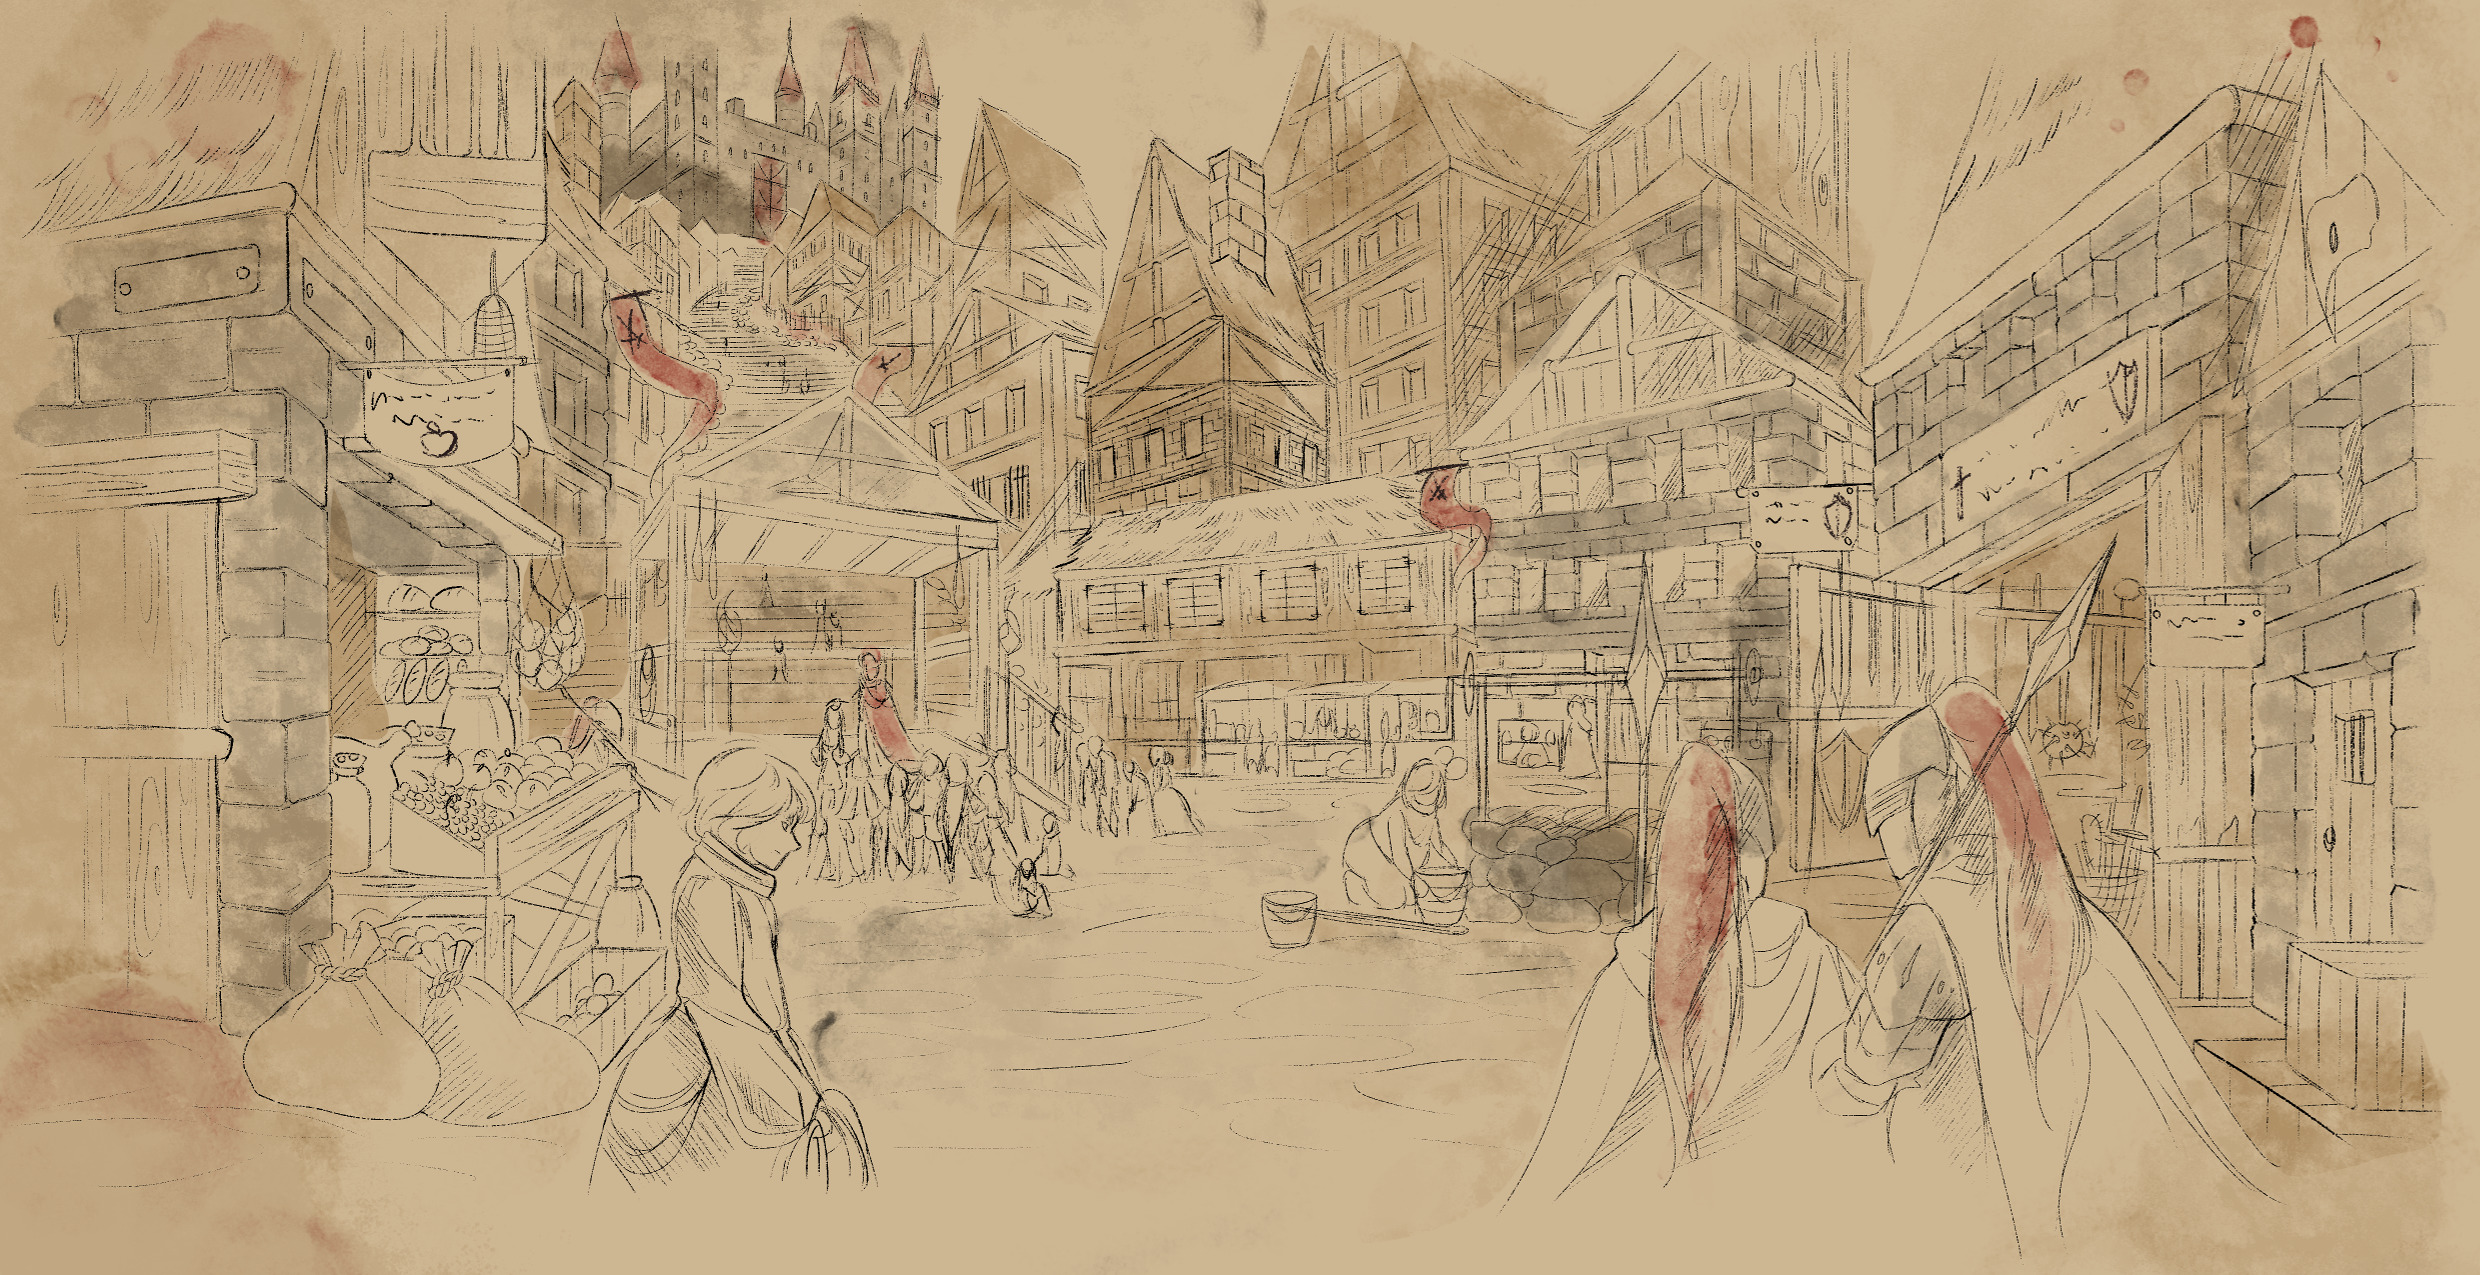
\includegraphics[width=\paperwidth,keepaspectratio]{media/norburysm.png}
  }
  \par
  Market place in \emph{Norbury}, circa GT:2102
\end{figure*}

\subsection{Norbury}
\label{sec:Norbury}

\graham{Surely the most vile city kingdom Aror has to offer...}
\aren{Bless thy innocent heart, for you have not lived long enough to see the
  rise of Morkan.}

The second youngest city kingdom, \emph{Norbury} resides on a large island off
the northern coast of the continent \nameref{sec:Eilean Mor}. Norbury is a
large walled city, encompassing a large part of the centre  of the huge island.

\subsubsection{History}

It was founded around \emph{GT:1849} as a joint military outpost of
\nameref{sec:Hraglund}, and other northern baronies of Eilean Mor. It was
originally intended as first line of defence against the many raids of the
beast races that came from the northern most continent of
\nameref{sec:Iafandir}. Quickly the fortress of Norbury grew into a castle,
and more and more people were required to keep the castle and its army
supplied. Armies need smiths, smiths need smelters, smelters need coal huts
and miners, and all of these need food, lodging and entertainment. Within a
few generations Norbury exploded in size and population, all working towards
one goal: keeping the raids and incursion of the beast races away from the
main continent.

By \emph{GT:2041} the city had surpassed baronies in sheer size and population,
and was granted the official status of a \emph{city kingdom}.

\subsubsection{Banner}

\begin{figure}[!ht]
  \centering
  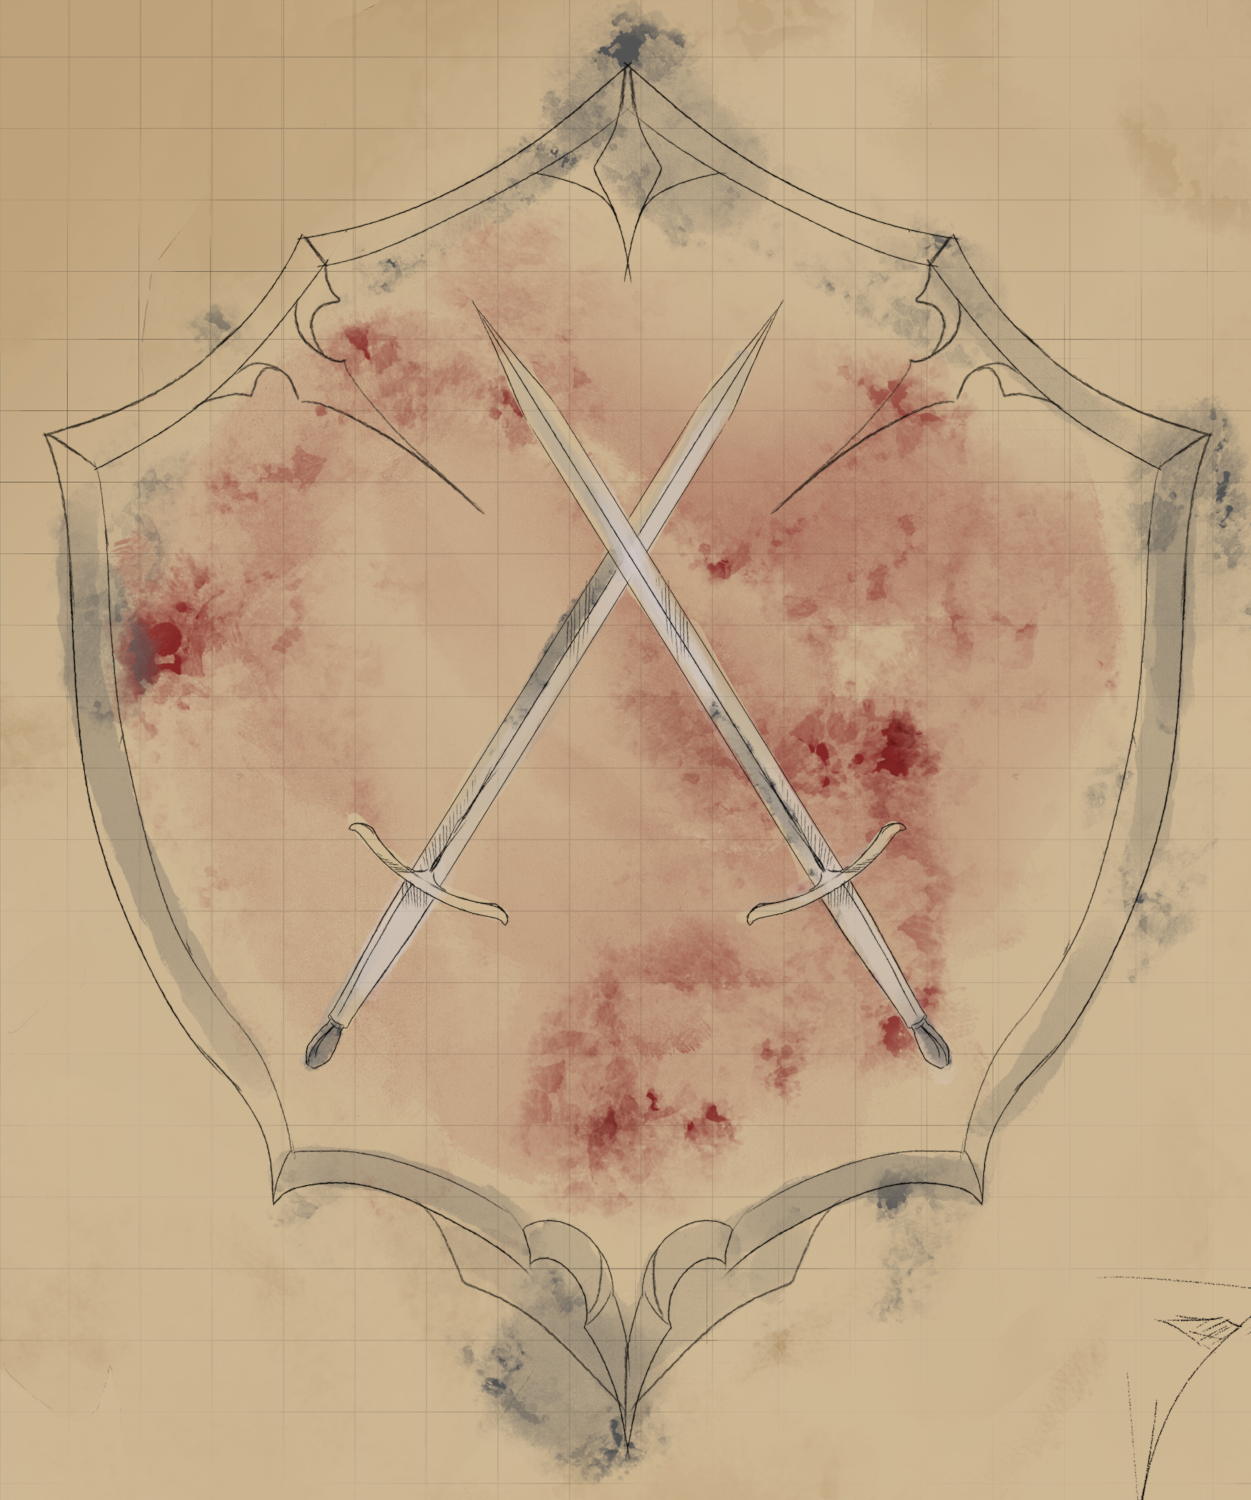
\includegraphics[width=0.9\linewidth]{media/norbury-bannersm.png}
\end{figure}

The kingdom's banner shows two silver swords crossed at the blade, against a
light red background. The main colours of the kingdom are silver and red.

\subsubsection{Districts}

The centre of the city is a large market place, with a big stone steeple in
the middle. The tower both signifies the eternal vigilance, but also houses a
large bell that is rung in case of an attack. Inscribed into the walls of
the steeple are the laws of the kingdom for everybody to read. The market
place is vast circular open courtyard, and all sorts of goods - including
slaves - are sold there.

To the north lies \emph{Norbury} castle, a huge fortified military camp and
seat of the monarch. It oversees the north eastern sea off the island, and
rests upon a roughly one hundred metre high cliff side. The castle district
also houses the richer barons, lords and ladies of the nobility of Norbury.

Further north west and south east lie the two major harbour districts that
the kingdom uses to maintains its vast fleet. Although these harbours are also
major trading hubs, they also house a majority of the city's working class or
poorer slaves.

To the south west lies the ``outreach'', a sprawling suburban district in which
the bulk of the Norbury citizens life. Both rich, poor, worker, artisan and
slave share this vast cityscape and life there together. Even though it is
called the ``outreach'' or ``outskirts'' this suburban area is still within
the city walls.

The surrounding area of the walled city houses farms and smaller villages that
also belong to the city kingdom. These farms are not walled, and thus
exposed to surprise sea raids from smaller vessels. The city provides these
outlying farms with watchtowers, patrols and sometimes even with full army
support are thus rarely defenceless.

In \emph{MI:1910} Norbury expanded its territory onto the mainland of Eilean
Mor. After the coastal barony surrounding castle Rothorn fell into disarray
when their old baroness died, the city kingdom invaded and claimed the land.
Norbury now holds and owns a small patch of costal area at the northern foot
of the \nameref{sec:Great Divide}.

\subsubsection{Sea Raids}

A network of watch towers, light houses, guard towers and scout ships
constantly check the sea north of \nameref{sec:Eilean Mor} for any impending
sea raiders that embark from the continent of \nameref{sec:Iafandir}. If a
suspicious ship or raiding party is discovered, the entire kingdom goes on
high alert and deploys their fleet. Norbury are excellent ship builders,
sailors and warriors on the sea; and so they prefer to capture and destroy
raiding parties before they land on Eilean Mor. Most of the ships manned by
the beast races of \nameref{sec:Iafandir} are often inferior in design, and
thus unfit for prolonged sea battles. Many are sunk off the coast of the
continent. The raiders that survive are fished out of the sea and then brought
back to Norbury.

There is a common misconception that Norbury enslaves all raiders that land
at the shores of Eilean Mor. But the city only enslaves those that actively
attack them, or raid coastal villages and towns as a way to make the raiders
repay the damage they have caused. Those that sail from \nameref{sec:Iafandir}
unarmed, or surrender, are more often than not escorted back to the savage
lands.

Sometimes raiding parties do sneak past the ever vigilant eye of the city,
and then land on the northern shores of Eilean Mor. Most of the baronies
on the shores have increased their armies to repel these raids upon their
lands. Yet some also call the mainstay army of Norbury for aid. Then the
soldiers of the barony attempt to bar the raiders from entering their land,
while the ships and navy of Norbury attack the landing party from the sea.

Defending Eilean Mor (the ``home land'') from sea raids is a cultural goal and
ideal, that is extended to any barony on the main continent. Some warriors of
Norbury even see it as impolite to ask for compensation or gold in exchange,
as there is enough honour already in defending their brethren of the main
land. Still many baronies and smaller earldoms pay Norbury for their aid,
either in gold, everblack or in trade deals highly favouring Norbury. Rivalries
that the city kingdom might have with the neighbouring baronies will not
hinder it to come to their aid in case of a raid from the sea.

\subsubsection{Religious Civil War}
\label{sec:Religious Civil War}

Ever since its foundation, the religions surrounding \nameref{sec:Lor}, the
\nameref{sec:Order} and the \nameref{sec:Three Kings} vied for the position of
dominance within the city. The Order had the most followers, followed by Three
Kings and then Lor. Although the priests and paladins of Order raised issues
with mistreatment of slaves, they were not outright against slavery unlike
the priests and followers of Lor who wished to see the practice banned. The
followers of the Three Kings found both the followers of Lor and the Order to
be weak in the face of their common enemy from the north, and were ready to
expel both religions from the city. Over centuries this conflict hardened and
brewed in the heads of the followers and citizens. Then, in \emph{MI:1480}
when a follower of the Three Kings beat his slave to death with a pavement
stone in the middle of the market place for disobeying him, a paladin of Lor
interfered by killing the slave owner in single combat. This event brought a
spark to the already volatile mix of religious animosity. The followers of the
Three Kings moved in retaliation against the temple and followers of Lor. The
Order, who sided with the mistreated slave, joined the conflict on the side of
the followers of Lor. A religious civil erupted that war lasted for two
months, in which both the Order and the followers of Lor suffered heavy losses,
and ultimately defeat, against a well-trained, well-equipped force inferior in
numbers. To prevent the bloodshed to spilling over to civilians, the then
ruling queen \emph{Arianna of Nordholm}, banned the religions associated with
Lor and the Order, and exiled their followers for being ``weak in the face of
adversity''.

Even though this conflict has long passed, the prevailing attitude in Norbury is
that followers of the Order and Lor were, and are still, weak and not worthy
of honour. Although the ban is still in place, the exile has since been
lifted, allowing priests and paladins of the two gods to visit the city.

\subsubsection{Culture}

Since the incursion and raids of the beast races still occur to this day, and
have grown to be more ferocious and demanding, the culture of Norbury has
grown in response. Norbury is from the lowliest slave and peasant up to the
king or queen herself, a meritocracy. You are worth as much to the city, and
in the eyes of your fellow citizen as you can contribute to the well being of
the entire whole.

Men and women of Norbury pride themselves in the work they are contributing to
the collective defence effort, be it front line combat, creating weapons and
armour for those that do, or aiding the effort in an administrative
fashion. Warrior culture runs strong in the kingdom, their deeds are sung in
taverns, and their likeness is made eternal in art. Many fighters and warriors
of Norbury follow the \emph{Three Kings}, although worship of \emph{Forun} is
also wide spread in the kingdom.

Although arcane and divine magic is still frowned upon in the kingdom, the army
of Norbury runs an academy for battle mages and wizards. Arcane research is
often scrutinized by its potential military application, and wizards are also
required to undergo basic military training in weapons and armour.

All citizens of Norbury (and those that wish to become citizens) must complete
a mandatory civil service of at least five years. Many use this mandatory
service to begin an apprenticeship, while others join the military to counter
raids and incursions. No one is excluded from this service, not even the
children of the reigning monarchs. Avoiding this service is not only illegal,
but is also seen as a major dishonour.

\subsubsection{Society}

Titles within the kingdom's society, such as commoner, earl, baron or even
duke and grand duke can be bought by any citizen of Norbury. There is a rather
unusual twist: These titles are not inherited, which means that the son of a
duke is a commoner upon birth. The common census is, that this child has not
done anything yet to earn the rank of earl for him or herself. There is a high
pressure on children to achieve the same status as their parents, or perhaps
even outperform them. Failure is always an option as well, as it is not
unheard of for a noble son to fall into slavery.

Who reigns as king or queen is decided in a ritual combat between all eligible
arch dukes that wish to rise to the challenge. This combat is not to the
death, although many grand duke's have perished in their claim for the
kingdom. A king or queen reins until his reign is challenged by another, or
until they die or resign. The people of Norbury mostly do not care what race
or social background of their king or queen, but instead judge all their peers
by their honour, combat prowess, and contribution to society as a whole.

\subsubsection{Slavery}
\label{sec:Slavery in Norbury}

Norbury is the foremost kingdom to practice slavery on a massive scale. Both
\hyperref[sec:Indentured Servitude]{indentured servitude} and
\hyperref[sec:Unregulated Slavery]{chattel slavery} are encoded in Norbury
law.

Many of the raiders that are captured, and most of those that commit major
crimes are enslaved. The wizard academy has constructed special
\hyperref[sec:Slave Band]{arcane collars} that bind the slave to their
owners. Slavery is rarely a sentence for life, as there are a few legal ways to
escape slavery. Slaves may be released at any time by their owners, those in
indentured servitude may buy themselves free, and state-owned slaves may be
simply set free once they can no longer contribute in any meaningful way to
society. However Norbury slaves (as compared those in servitude) have no
rights whatsoever, and are marked, colour coded, registered by number, and
tracked down by the \nameref{sec:Hunters Guild} should they decide to
run. Slave collars allow slave owners to track, command and often punish their
wearers.

Foreigners are allowed to purchase slaves, however they have to pay an
additional fee half the slave's value. This was intentionally done, so that
most of the slaves remain within the city and contribute to the city. Slave
ownership is recognised as lawful in all kingdoms and baronies that have
signed the \hyperref[sec:Vonir Accord]{Vonir Accord}.

Although the city has a large slave population (between 20 and 30 percent),
it rarely faces slave revolts or uprisings. There are four main pacifiers at
work that keep the slave population suppressed and obedient. First, for many
slavery is potentially only temporary. Many are forced to join the Norbury
army, the Hunter's Guild or begin work in other positions that would qualify
them for citizenship later on, and thus do not wish to risk their permanent
freedom through revolt. The second is a ever permeating culture of honour and
duty, especially in the still ongoing sea raids from the north. Many slaves
derive a sense of purpose from working toward a common goal. Also many
churches and charitable organisations provide a network of services and goods,
such as food, warmth and medical services to slaves making their lives
bearable. Although gatherings of slaves are forbidden, the Hunter's Guild
often looks the other way in regard to slave bars or inns, as long as no
direct threat stems from these establishment. And the fourth reason is the
ever vigilant \nameref{sec:Hunters Guild}. Their network of informants,
hunters, and agents quench any rebellious flame that might kindle in the dark.

\subsubsection{Spinetails}
\label{sec:Spinetails}

However the city also has a certain societal class of slaves that have slipped
through the crack of the Hunter's Guild. Those are slaves that were deemed
valueless, cannot work because of disease, illness or handicaps, are mentally
unstable or even violent, or may have lost their owner and thus no one lays a
claim on them. Their collars often show the colours ``white'' (valueless) and
``red'' (without owner), and are thus often named ``spinetails'' after the
bird that wears the same colours in its feathers. Spinetails hide within the
vast sprawling suburbia of the city from the guild, and survive by committing
petty crimes, begging or from aid given to them by generous people and
organisations. They have since begin to form their own societies, subculture
and even their own crime organisations. The Hunter's Guild warns anyone from
claiming a spinetail as a slave, and rewards citizens should they turn them in
or give hints that lead to their apprehension. Generally spinetails are viewed
as a problem by most citizens, and most owned slaves. Disease, drug abuse, and
crime is rampant within Spinetail subculture, and many see them as free-riders
and slackers.

\subsubsection{Population}

Norbury, and its outlying villages, houses roughly 4 million people. Of which
the vast majority are human and deepkin (39\%), then elves (24\%) followed by
dwarves (15\%) and half races (10\%). The rest (12\%) are beast races, almost
all of which are enslaved. Roughly 31\% of the entire population is either
currently enslaved or in servitude.

%% City Kingdom of Stenheim
\cleardoubleevenemptypage

%% TODO: Artwork

\begin{infobox}{City Kingdom of Stenheim}
  %% TODO: Crest
  \begin{multicols}{2}
    \begin{itemize}[label={},noitemsep,leftmargin=0.0cm,topsep=0pt]
      \infoboxitem{Location}{North western shores of \nameref{sec:Goltir}
      }
      \infoboxitem{Languages}{Doresh, Teranim, Old Teranim}
      \infoboxitem{Government}{Absolute Monarchy}
      \infoboxitem{Major Religions}{\nameref{sec:Forun}, atheism}
      \infoboxitem{Area}{est. 60,000 $km^2$}
      \infoboxitem{Population}{est. 19 million people}
      \infoboxitem{Non Grata}{monstrous races (including Gorgons), druids,
        devils
      }
      \infoboxitem{Magic}{All forms of magic overseen by the government, who
        grants permits and sets limitations
      }
      \infoboxitem{Slavery}{outlawed, indentured servitude available as an
        option to criminals to reduce sentence, imprisons criminals
      }
      \infoboxitem{Special Laws}{only state that allows sentient golems to
        become citizens
      }
      \infoboxitem{Notable Organisations}{\nameref{sec:House Ranian}, remnants
        of the ancient Deepkin houses
      }
      \infoboxitem{POI}{Central market, university of applied sciences and
        engineering, mountain plateau that is a recreational park, largest
        telescope on the northern hemisphere
      }
    \end{itemize}
  \end{multicols}
\end{infobox}

\clearpage

\subsection{Stenheim}
\label{sec:Stenheim}

The city kingdom of \emph{Stenheim} (also ``Stoahom'' in some local dialects)
lies on the north western shores of \hyperref[sec:Goltir]{North Goltir},
situated on the foot of the coastal mountain range of the Aldenes, where the
Taraun river flows into the sea. While the majority of the newer city has been
built at the foot of the mountain, the old city centre, the castle and main
fortifications reside in natural and hewn caverns in the mountain.

The city's banner features a red dragon upon a white shield, crowned by a
three pronged red crown. Red and white are the nations colours, representing
the iconic skin and hair colour of the \nameref{sec:Deepkin}.

\subsubsection{History}

It was officially recognised as a city kingdom in GT:1551, but is considered
far older. Earliest record dating back to almost GT:531 were found in the
vault of the city, albeit it was but a small deepkin settlement back then. It
began as a small tribal city, but soon the favourable conditions of the
settlement's location, namely access to the shore and fresh water from the
river, attracted more and more deepkin, and dark elven clans. Unlike most of
the dwarven clans that lived in the Aldenes, the deepkin clan welcomed their
surface brethren into their deep caverns from the beginning.

The deepkin built another smaller city outside their caverns, and used it to
trade the ores and gemstones to the other nations and kingdoms. The access to
the river, the easy connection to the sea (and thus trade), and its beautiful
and scenic lake scenery attracted more and more of the surface races, and the
city grew over the course of many centuries.

\subsubsection{Wars}

The kingdom was involved in many defensive wars over the course of its early
history. Many dwarven clans, especially the \emph{Black Hill} and
\emph{Snowhammer} clans, as well as remnants of the various Ilian empires of
the deep tried to seize the deepkin workshop. None of these assaults and sieges
was successful, and nowadays the kingdom of Stenheim has eclipsed all dwarven
and Ilian clans in size and power.

The deepkin had used their ingenuity to construct advanced war machinery such
as arcane siege weapons, arcane weapons and armour, as well as war golems to
defend their home. This distinct technological advantage helped them defeat
their aggressor, even though they often had superiority in numbers.  This
technological advantage did not sleep, and still to this day the city kingdom
is considered one of the strongest in terms of military power, capable of
fielding an army well equipped with arcane gear, as well as countless combat
ready golems, as well as arcane war and siege machinery.

Compared to many other more warring clans of the Aldenes, the deepkin never
enslaved or seized the lands of other clans. Most of the wars the deepkin
thought were defensive in nature. Their less aggressive approach, as well as
their propriety to get along, diplomatically and culturally, with the other
deep races made their kingdom an attractive destination for the other mountain
clans. Many smaller dark elven, and dwarven clans migrated to the city and
integrated well into the deepkin culture.

\subsubsection{Population}

The outlying city of Stenheim, as well as the deepkin workshop and castle holds
roughly 19 million people, of which the majority are deepkin (39\%) and dark
elves (22\%), while humans (11\%), elves (10\%), while halflings (4\%) and
dwarves (3\%) make up the minority. Due to the deepkin's liberal and welcoming
nature, Stenheim has become a destination for many half races (9\%) as well as
undead (2\%).

The city also uses humanoid-like golems for dangerous tasks such as city
defense, or difficult menial labour such as mining, construction or hauling.
They are called ``Homunkulus'' within the city, but outsiders know them mostly
from the many defensive wars where they earned the nickname ``Warforged''. The
vast majority of these golems are nothing more than well programmed, and
arcane automatons made of steel and Everblack. But some have gained
consciousness and self-awareness. Stenheim has retroactively freed and
liberated all self-aware Homunkulus from servitude, and given them citizen
rights within the kingdom.

Common male names are: Adrian, Alex, Andreas, Anselm, Arnold, Axel, Baldur,
Benjamin (Ben), Björn, Eckbert, Eduard, Erik, Erwin, Felix, Florentin
(Florian), Franz, Gisbert, Gregor, Gustaf, Heinrich, Helfried, Johannes
(Johann, Hannes), Karl, Klaus, Kilian, Lars, Leo, Lukas, Matthias,
Maximilian (Max), Nicklas (Nick), Oliver, Othmar, Patrick, Rafael, Reinhold,
Samuel, Sieghard, Sigismund, Torben, Valentin, Wolf

Common female names are: Abigail, Ada, Adelina (Lina, Adela), Alexandra (Alex,
Alexa), Amelie, Anna, Brigitte (Birgit), Daniela (Nela), Edit, Eleonora,
Elisabeth (Elisa, Elli, Lisa), Emma, Eva, Evelyn, Hanna, Helena, Ida, Ina,
Irene, Irma, Jana, Julia, Karla, Katarina (Katrin), Leah, Magdalena (Lena),
Margareta (Greta, Grete, Gretchen), Manuela, Mia, Ria, Rita, Roswita, Sara,
Sofia, Verena, Viola

\subsubsection{Culture}

The deepkin of Stenheim (and by extension the other races living there as
well), are predominantly atheistic. Only Forun and the other holy mothers have
a sizeable following within the mountain kingdom. The city mostly focuses on
mining and arcane research, and the people of Stenheim pride themselves for
being a centre for scientific and arcane learning.

Most people of the kingdom are considered humble, curious and known for their
love all things science and engineering. The deepkin have shared their passion
for golem construction, mechanical and civil engineering with the other races
that joined them. Almost all people in the kingdom enjoy luxuries that no
other kingdom can offer, such as indoor plumbing, arcane light fixtures and
cheap commodities due to early attempts at mass production.

The culture of Stenheim is known for being one of the most liberal and
advanced of all the city kingdoms. The people enjoy a wide variety of social,
economical freedoms, as well as a fair, stable and efficient state and legal
system.

\subsubsection{Rule}

The kingdom is lead by a patriarch or matriarch which is elected by council of
city elders, guild leaders, high ranking professors from the arcane academy,
as well as constabularies that are chosen by the general population through
votes. This ruler is then sworn in, and stays in power until his or her death,
abdication or until the council elects to vote for a new patriarch or
matriarch. Although not technically a queen or king, the ruler of the city is
deemed equal to a king or queen by the other city kingdoms and welcomed as
such.

More unusual is the fact that the kingdom is split into smaller districts,
each ruled by a constabulary. Although these local rulers report to the
matriarch or patriarch, they hold considerable power within their district,
and are even allowed to pen local laws. They are voted into office by the
people of their district, albeit the matriarch can remove a constabulary from
power.

The city's population and the majority of their rulers are against slavery,
and has also removed indentured servitude in favour of imprisonment. Convicted
criminals can still opt to reduce their sentence by mining for ore, or reduce
their sentence even further by mining for \nameref{sec:Everblack}. The kingdom
did not sign the \nameref{sec:Vonir Accord}, but most of their citizen are
well protected from slavery in other kingdoms as no foreign power wishes to
risk a diplomatic incident with Stenheim.

\subsubsection{Relations}

The kingdom holds good relations with the other city kingdoms, except for
Kesmar. Stenheim often accused the dwarven kingdom for secretly aiding their
enemies during past sieges and skirmishes. Most of surrounding dwarven clans
in the mountain hold the kingdom in contempt, seeing them as an imperialistic
force with no equal in power. Even though the kingdom does not aggressively
expand, the surrounding clans and tribes are pressured into joining the city
or face becoming irrelevant next to their neighbour.

Furthermore Stenheim is known for exporting both their advanced war machinery,
technology, ore and everblack to other nations. It is known for selling their
weapons and golems to anyone who are able to front the price.

%% City Kingdom of Tredegår
\subsection{Tredegår}
\label{sec:Tredegar}

The city kingdom of \emph{Tredegår} (old-high Teranim for ``three courtyards'')
lies on the south western shores of \emph{Eilean Mor} west of the \emph{great
  divide}. It is encased by two large rivers: The \emph{Morre} river to the
north and west, and the \emph{Moy} river to the east and south. It's close
proximity to the mineral wealth of the great divide, the easy access to two
rivers and the sea made Tredegår one of the richest city kingdoms of all of
\emph{Aror}.

\subsubsection{An'Rath}

In the centre of the city is the vast castle of \emph{An'Rath}, which houses
roughly a thousand people. Workers, nobles, clergymen, bureaucrats, judges,
advisers, as well as the ruling family live within the castle. The castle by
itself is an impressive architectural feat, and is constantly being extended
with additional towers and buildings. The castle has its own army, and its own
inner stone wall for protection, and even inner draw bridges and gates to
separate individual parts from one another in case of a siege. The outer ring
of the castle is open to the public, and houses a library, a school that
offers various courses, its own brewery and tavern (\emph{The Drunken Trader}).

\subsubsection{Banner}

The banner of Tredegår features a white tree with three thick branches resting
within a shield. A golden crown rests above the shield. Gold, white and blue -
representing the gold of the great divide, the white snow up on their peaks,
and the blue rivers and the sea - are the colours of Tredegår.

\subsubsection{Population}

Among all the city kingdoms Tredegår is by far the biggest. It houses roughly
32 million inhabitants, with all the outlying villages included. Most of these
are humans (55\%), with dwarves that once lived in the great divide following
close second (21\%) followed by elves (10\%), half races (12\%) and various
others (2\%).

\subsubsection{Culture}

The immense wealth of the city has trickled down to most of the lower and middle
class citizens. Thus the people of Tredegår live in an unparalleled state of
social security that is only known in that kingdom. Most people of the city
work far less than their contemporaries in other kingdoms. Still they make
enough money to life comfortably. This gives the people of Tredegår time and
opportunity to enhance their education and other skills. The people of Tredegår
are often described as well educated, easy going and relaxed; with strong focus
on self improvement and family. Some have described them as arrogant and snobby,
although those attitudes can often be exaggerated by envy. A typical Tredegår
craftsman for example works slow, meticulously and prefers to deliver quality
over quantity. This culture of ``do it right; or do not do it at all'' has
earned the city a good reputation as a reliable trading partner that delivers
excellent product.

This culture is also present within the kingdom were houses, streets, bridges
are seldom derelict or run down. Instead they are always lavishly decorated with
flowers, and the city maintains a network of arcane street illumination housed
in lamp posts. Public workers keep the streets clean and make sure that the
city always Although the city as no slum or worker district, poverty does
still exist within the city, especially among the sick and crippled.

\subsubsection{Steel and Smithing}

The \emph{Tredegår Steel and Gold Corporation} is one a large company that
runs many forges and smithies across the city. It works off the raw ore mined
either in the great divide, or ore that has been brought in from the
\nameref{sec:Silver Isles}. The corporation is known for its excellent
craftsmanship in weapons and armours, and their products are sold all across
the major kingdoms and are renowned for their quality and steep price.

\subsubsection{Society}

Without the economical pressure due to the immense wealth of the city, slavery
has been abolished several centuries ago. The city has been ruled by the same
noble family \emph{Gylleborg} for thousands of years. Both female and male
heirs may rule. The city kingdom has a long history of peace and prosperity,
and the justice system is known all around the world as one the best of its
kind. Independent judges and prosecutors work in tandem with private defence
attorneys to ensure the justice system remains fair and independent.

\subsubsection{Relations}

The city and its nobility is closely related to \nameref{sec:House Ranian},
and the house has the main headquarters near the main square of the city.

Due to their status as rich trading partner, the city kingdom of Tredegår is
in good standing with almost all other city kingdoms, except \emph{Morkan}.
Their longest standing trading partner and ally is the city kingdom of
\emph{Fes al-Bashir} to the south. The city kingdom strengthened their bond
with the other city states by providing logistical advisers, money and
their best smiths during the rebuilding of \emph{Forsby}. The kingdom is a
signer of the \emph{Vonir Accord}.



% Characters
\section{Characters}
\label{section:Characters}

% Aren Fel
\subsection{Aren Fel}
\label{sec:Aren Fel}

Aren Fel of \nameref{sec:Nicte}, most commonly known as the ``Undying Witch''
(born sometime around GT:24) is a \hyperref[sec:Deepkin]{Deepkin}
\hyperref[sec:Soul Magic]{soul witch}, priestess of the \nameref{sec:Silent
  Queen}, thief, diplomat, author, historian and scholar.

Her family tree, blood line, birth and association with House Nicte have been
thoroughly documented and dated to GT:24. She was born to small deepkin
commune, which now lies within the kingdom of \nameref{sec:Stenheim}. And even
though she possess new female deepkin bodies to stay alive over the aeons, her
continued longevity as been independently confirmed by several other
long-lived species, including vampires, dragons and even giants, who were able
to recognise her unique soul across the centuries.  This is also why her
appearance is not described, as it would be a fruitless labour.

Initially born into the Nicte family clan, she was trained preliminary as a
diplomat, thief, spy and trader. As the battles of the aeon of strife came
closer to her family, she was also hastily trained in combat, and joined the
skirmishes as an archer and scout. She suffered a major trauma and wound during
those skirmishes, which also \hyperref[sec:Soul Awakening]{broke her soul}.
After her clan realised her condition, Aren was sent off to be healed by the
\nameref{sec:Walburga} witches. Aren took the opportunity to learn as much as
she could about soul magick from them, including how to possess other people
or bodies. Although she was inducted into the coven as a witch, she was
ultimately asked to leave due to her allegiance to a lesser deity. Aren still
uses this power by possessing newer, younger bodies to prolong her life.
Although the races she inhabits now vary, she always remains female.

During her unnaturally long life-span she used her extensive
training from her Deepkin clan to forge alliances, gather artefacts,
manoeuvre political developments, and to manipulate the rich and powerful.
She consolidated many smaller baronies, bolstered their political and military
power, and directly steered many of them to join or start wars that would see
an end to the strife on Goltir. Aren achieved this goal over the course of
several centuries by holding high ranking offices, such as adviser to the baron
or baroness. She was thus instrumental in the early history of the
north-western part of \nameref{sec:Goltir}, by making sure the core humanoid
settlements remained allied with each other. Aren was instrumental in paving
the way for both Stenheim and \nameref{sec:Forsby} to rise to be global
powers.

She was also heavily involved in the \nameref{sec:Holy Crusade}. There she
managed to lessen the extend and cruelty of the crusade by actively opposing
the persecution of low-ranking followers of Griannar, including the general
congregation and low-ranking acolytes. Aren directly stood against her own
high-priestess \nameref{sec:Aria}, causing a schism within the church of the
\nameref{sec:Silent Queen}. Between the warring faction following Aria on one
side, and the more neutral, and pacifist congregation that followed Aren, on
the other. Aren further aided \nameref{sec:Hraglund} during the plague, and
assisted the kingdom in finding a cure by securing the help of important
arcane institutions including the \nameref{sec:Hall of Knowledge} and
\nameref{sec:Magistrata Arcanum}. The last recorded appearance of Aren was
during the siege of Forsby, where she smuggled \nameref{sec:Everblack Golem}
made by Stenheim into the city to help with the defence against the devils.

Although her achievements are well recorded, so are the means by which she
attained them. Aren is notorious for her Machiavellian scheming, and often
pursuing careless and reckless plans, in which she prioritises a quick and
satisfactory end of the crisis at hand above anything. Her philosophy that the
ends justify the means, has lead to her to commit blackmail, theft, slavery,
and even murder. She is often accused of showing a blatant disregard for the
lives of others, for example by killing the souls of future hosts simply to
extend her own lifespan, or by deliberately starting wars during the
strife. Her many, and well documented crimes, has made her an enemy of many
judicial organisations, such as the church of \nameref{sec:Lor}, or the church
\nameref{sec:Order}. She is furthermore a persona non grata in four city
kingdoms: Fes al-Bashir, Forsby, Hraglund, and Tredegår.

\label{sec:Witch Hunt}
The power she wields, both literally as a powerful soul witch, and
figuratively through her web of alliances, caused a lot of animosity and open
hostility from other powerful organisations. In MI:20, after the Holy Crusade,
the \nameref{sec:Knight Order of Tavos} attempted to catch, trial and execute
Aren. A literal witch hunt began, that lasted from MI:20 to MI:28 that caused
many innocent Deepkin women harm, caused them to lose their freedom and even
their lives in an attempt to bring Aren to justice. This is period of time is
now known as the ``Witch Hunt'', and is considered the sole fault of the Knight
Order of Tavos.

Nevertheless her knowledge of the world, its inhabitants, the creatures and
threats of the planes, arcane, and soul magic is extensive, as is her web work
of power, alliances, and ability to influence even the most powerful
organisations. As a member of \hyperref[sec:Two Courts]{Court of the Suns},
she is very often asked for aid, when a global crisis afflicts Aror.

\begin{note}
  Aren can serve many purposes in your campaign: she can be the secondary
  villain, prime villain, or simply be an aid to the party, preparing them
  to face the actual villain. She will \emph{never} work towards the doom of
  Aror, or its citizens on purpose, but will use \emph{whatever means
    necessary} to achieve goals. Even though these goals may overlap with
  that of a good PC party (i.e. saving the world), her methodology and
  philosophy make her an evil character in terms of D\&D alignment.
\end{note}

\begin{35e}{Aren Fel 1 Fighter / 17 Rogue}
  \srditem{Size/Type}{Medium Humanoid (Deepkin)}
  \srditem{Hit Dice}{2d10 + 15d6 (79+36) 115 HP}
  \srditem{Initiative}{+3}
  \srditem{Speed}{30 ft.}
  \srditem{Armour Class}{}
  \srditem{BAB / Grapple}{+12/+19}
  \srditem{Attack}{}
  \srditem{Full Attack}{}
  \srditem{Space/Reach}{5 ft./5 ft.}
  \srditem{Special Qualities}{Dark Vision (120 ft.)}
  \srditem{Class Features}{Sneak Attack (+9d6), Trap Finding, Penetrating
    Strike (ACF), Improved Uncanny Dodge, Improved Evasion, Skill Mastery (Use
    Magic Device)
  }
  \srditem{Soul Power Points}{1d6+15d8 (80+144) 228 SPP}
  \srditem{Soul Powers Known}{All of them}
  \srditem{Saves}{Fort: +8, Ref: +10, Will: +5}
  \srditem{Abilities}{STR: 30, DEX: 16, CON: 14, INT: 16, WIS: 12, CHA: 26}
  \srditem{Skills}{Bluff (+30), Diplomacy (+29), Disguise (+19), Hide (+4),
    Intimidate (+21), Knowledge (local) (+21), Knowledge (Planes), Knowledge
    (Soul Magic) (+17), Move Silently (+4), Search (+19), Sense Motive (+19),
    Soulcraft (+17), Spot (+19), Tumble (+4), Use Magic Devise (+21)
  }
  \srditem{Feats}{1: Able Learner, 2: Improved Initiative, 3: Radiant Soul,
    6: Power Attack, 9: Craven, 12: Staggering Strike, 15: Combat Reflexes, 18:
    Robilar's Gambit
  }
  \srditem{Items}{Aren's Grand Seal of Nicte [Ring] (+10 Diplomacy, +10
    Bluff), Aren's Remembrance [Ring] (+8 Charisma, +8 Strength)
  }
  \srditem{Challenge Rating}{18}
  \srditem{Alignment}{Lawful Evil}
  \srditem{Advancement}{Rogue levels}
\end{35e}

% Eigyr
\subsection{Eigyr}
\label{sec:Eigyr}

Eigyr Waylin (born circa GT:-550, and died circa GT:-320) was a high elven
warlord, politician, shamaness of the \nameref{sec:Old Ways} that rose to
prominence in her campaign against the monstrous races on \nameref{sec:Eilean
  Mor}.

Her history, deeds, accomplishments but also most of her defeats and failings
are well documented in the stories, songs and traditions of the Old Ways. Within
humanoid traditions and culture of both the Eilean Mor, and the northern part of
\nameref{sec:Goltir} she is universally celebrated as a heroine, champion and
liberator. Her fame also stretches across the continents, and her tactics and
teachings have also been extensively studied by the scholars of Arania and
Avenfjord. Eigyr's fame turns into notoriety among the monstrous races, who see
her as conqueror and defiler of their lands.

In her early years she was an accomplished huntress, archer, and wielder of
two blades in each hand, and fought the monstrous races by leading small war
bands, and employing mostly hit-and-run tactics. Through many early victories,
and skilled diplomacy she rallied more and more villages and tribes behind
her. Soon she had a formidable army, and began to assault, and besiege larger
monstrous towns. Eigyr lost many of these earlier large scale battles, as she
failed to adapt tactics, and logistics from the small skirmishes she knew well,
to tactics and logistics required of a large and vast armies. Her pride and
bullheadedness are often attributed to those seemingly needless losses.  After
appointing new advisers, and generals to lead her ever growing armies the winds
turned again in her favour. She is remembered as a woman who fought with
honour and courage in battle, never taking lives of the innocent (be they
beast or men) and actively punishing her men and women if they committed war
crimes against the innocent.

Eigyr is described by many stories as a wise, natural, honour-bound and
charismatic leader, but also as a spiritual purist. She detested the worship
of lesser deities, especially the \nameref{sec:Three Kings} but also those of
\nameref{sec:Lor}, and \nameref{sec:Griannar}. The stories tell, that she often
refused to aid those that worshipped ``false gods'' or those that she felt were
without honour.

Her campaigns ended around GT:-390, after she had defeated all major monstrous
cities on Eilean Mor, and driven most monstrous tribes across the northern sea
to \nameref{sec:Iafandir}. Eigyr ruled wisely and justly over her newly formed
empire in the centre of Eilean Mor until her death. In her final years she
also often travelled her empire, telling her own story to the people. Eigyr,
becoming wiser in her years, never failed to mentioned her failings and lost
battles, urging people to learn from them. She especially regretted the
needless losses in the early sieges, brought on by her inability see that she
could not lead and oversee the grand army all by herself.

Many towns, villages, cities and even \hyperref[sec:Wayfaerers
  Guild]{organisations} are named in her honour, although her empire fell
apart soon after she departed. Most large humanoid city kingdoms and some
baronies of Eilean Mor owe their founding to her legacy. Also many of the
newer traditions of the \nameref{sec:Old Ways} are directly based on her
teachings, and retelling of her own story in her later years.

% Graham Balance
\subsection{Graham Balance}
\label{sec:Graham Balance}

Graham Balance, born GT:2084 somewhere in the Dirgewood, died GT:2139 in
\nameref{sec:Fes al-Bashir}, was one of the great polymaths of early Arorian
history. He was an accomplished writer, musician, historian, philosopher,
arcane wielder, politician and grand magus of the hall of knowledge.

As a young adult Graham travelled around the world, from his home in the
Dirgewood across the sea to Goltir, all the way down south, across Farlar, and
then met the dragons of Draigynus, before finally settling Arania. On his
pilgrimage across the world of Aror he penned the most popular, and most
widely printed and copied book on all of Aror: the ``Wayfaerer's Guide to
Everblack''. He also penned most of his other popular works, specifically songs
and poetry, both the originals, and those he collected from various cultures
around the world, on his year long journey. His songs are still sung today,
and his rhymes and words are still recited to the next generation so they are
not forgotten.

After arriving in \nameref{sec:Fes al-Bashir} he joined the \nameref{sec:Hall
  of Knowledge}, were his broad knowledge of the world earned him a teaching
position. As a professor for cultural history, ancient societies and languages
he taught several student generations, before deepening his understanding of
arcane magic, philosophy and science. It was at the academy where he wrote his
greatest work: ``The History of Divine Form'', which is a detailed treaty and
look on the old religions, true deities and their teachings. It also put forth
a hypothesis: that if enough people believe in a true deity, one might be
``willed'' into existence. It is in this book were he founded a new religion
and dogma, with another true deity at its centre: the \nameref{sec:Sea
  Priestess}.

After about fifteen years of professorship he rose to be the Grand Magus of
the Hall of Knowledge, and thus, in turn, became the most powerful political
figure in Fes al-Bashir. He ruled the city and the Hall of Knowledge until his
death in GT:2139. Although his reign was short, he moved both the Hall of
Knowledge away from worship of lesser deities, and towards the sciences. And
although internal power struggles within the cities prevented him from
enacting lasting change in the city, he is still remembered as a wise,
tempered, and just ruler of the city.

Graham balance is mostly remembered when he was Grand Magus. As a man in his
advanced years, short hair, a beard that reaches down to his chest and covers
most of his face. He had sharp blue eyes, a long elongated face, and was
decently handsome. His charisma stemmed from his sharp and eloquent wit, as
well as his commandeering presence.

% Irene de'Var
\subsection{Irene de'Var}
\label{sec:Irene deVar}

Irene de'Var, Countess of Saremen, is the current ruler of \nameref{sec:House
  deVar} of Saremen in \nameref{sec:Helmarnock}, and thus one of the five
rulers that make up the council of the city kingdom.

Irene is about two metres tall, and has short white dyed hair, deep and dark
red eyes, and blue finger nails that show her usage of \nameref{sec:Ramesk}.
Her origin as a \hyperref[sec:Snow Elves]{snow elf} has granted her with
natural grace and beauty, which she complements with elaborate and intricate
silken garments, expensive and impressive jewellery (both magic and mundane)
as well as graceful posture and mannerism.

The countess is seen as a cunning politician, and a passionate and genius
orator capable of inspiring and moving their subjects through speeches, and
using her commanding presence and eloquence to resolve conflicts through
negotiations. To her people she shows her warmer, more compassionate side,
often meeting her own subjects on festivities or other special occasions.

Originally a snow elf diplomat of Helmarnock stationed in \nameref{sec:Forsby},
she was turned into a vampire in MI:1081 by the Count Nareil of House de'Var,
to serve as an heir in his lineage of nobility. His nobility has roots back to
the time of the great betrayal by \nameref{sec:Morana} during the aeon of
strife, and was instrumental in establishing and defending the city on the
island of Saremen amidst the constant wars and battles fought against the
beast races. Even though the countess has been trained in classical sword
fighting, and especially fencing, she prefers diplomacy over war and conflict.

Irene has ruled House de'Var since MI:1121 after the death of Nareil. She has
since restructured and reformed the House, leading them to become the most
dominant noble family on the island. Irene largely follows the houses traditions
and Nareil's teachings, and stays true to Nareil's style of leadership of
benevolence and diplomacy: Irene outlawed slavery on Saremen in MI:1122
freeing all who were previously enslaved to a citizen of Saremen, and pushed
the council to allow \nameref{sec:Umgeher} and \nameref{sec:Gorgons} back into
the kingdom. The ban on slavery was partially effective, since the city
kingdom has signed the \nameref{sec:Vonir Accord} before her push toward slave
liberation. Even though no new slaves may be taken within Saremen, and all
slaves of Saremen citizens have been freed, slavers of other nations,
including the other islands of Helmarnock are still allowed to follow that
practice on Saremen.  She initiated a council vote on slavery, but was
defeated two to three.

Generally Irene de'Var attempts to drive the society of Saremen towards
individualism, liberty and freedom, lifting many restrictions both in the
social sphere - such as lifting marriage restrictions between mortals and
vampires, ending slavery or allowing Gorgons to become citizens - as well as
in the economical sphere by lowering taxes and making it easier for companies
to do business. Her political leanings and open policies, together with her
well-received, compassionate speeches towards her subjects, have made her a
well beloved and respected countess among the citizens of Saremen. Although
she is a brilliant politician and orator, she keeps a cadre of highly skilled
advisers as a ``council of ministers'' that oversee other aspects of the
island, such as defence, finances, civil engineering or oversee the Academy of
Arcane Arts.

\begin{35e}{Irene de'Var (13 Bard / 2 Fighter)}
  \srditem{Size/Type}{Medium Undead (Vampire)}
  \srditem{Hit Dice}{15d12 (98 HP)}
  \srditem{Initiative}{+13}
  \srditem{Speed}{30 ft.}
  \srditem{Armour Class}{40 (9 dex, 10 armour, 5 deflection, 6 natural), 24
    touch, 31 flat-footed}
  \srditem{BAB / Grapple}{+11 / +17}
  \srditem{Attack}{+24 +4 Rapier 1d6+6 18-20x2}
  \srditem{Full Attack}{+24/+19/+14 +4 Rapier 1d6+13 18-20x2}
  \srditem{Space/Reach}{5 ft./5 ft.}
  \srditem{Special Attacks}{Blood Drain (Ex), Create Spawn (Su), Energy Drain
    (Su)}
  \srditem{Special Qualities}{Scent (Ex), Feral Blindness (Ex),
    Damage Reduction (Su), Resistances (Ex) DR 10 cold and electricity,
    Spider Climb (Ex), Turn Resistance (Ex) +4, Fast Healing (Ex)
  }
  \srditem{Class Features}{Bardic music, Bardic knowledge, Countersong,
    Fascinate, Inspire courage +2, Suggestion, Inspire greatness, Song of
    Freedom
  }
  \srditem{Spells Known}{\emph{Level 0}: Detect Magic, Fleeting Fame, Ghost
    Sounds, Dancing Lights, Prestidigitation, Read Magic

    \emph{Level 1}: Improvisation, Invisibility (Swift), Silent Image, Identify

    \emph{Level 2}: Alter Self, Detect Thoughts, Invisibility, Suggestion

    \emph{Level 3}: Blink, Haste, Dispell Magic, Halt

    \emph{Level 4}: Dimension Door, Freedom of Movement, Invisibility
    (Greater), Blinding Beauty

    \emph{Level 5}: Dispell Magic (Greater), Cacophonic Burst (Greater)
  }
  \srditem{Saves}{Fort +12, Ref +22, Will +26}
  \srditem{Abilities}{Str 22, Dex 28, Con -, Int 18, Wis 22, Cha 36}
  \srditem{Skills}{Bluff (+39), Intimidate (+41), Perform (Oratory) (+31),
    Perform (Dance) (+31), Diplomacy (+41), Gather Information (+31),
    Knowledge (Arcane) (+22), Knowledge (Royalty \& Nobility) (+22), Knowledge
    Local (+22), Sense Motive (+42), Spellcraft (+22), Hide (+17), Move
    Silently (+17), Search (+12), Listen (+14), Spot (+14)
  }
  \srditem{Feats}{Force of Personality, Leadership, Extend Spell, Metamagic
    Song, Improved Weapon Finesse, Improved Initiative, Weapon Finesse,
    Heighten Spell}
  \srditem{Items}{Royal Regalia of Saremen (+8 Charisma, +10 Armour Class),
    Seal of Saremen (+5 Resistance, +10 Diplomacy, +10 Sense Motive), Crown of
    Saremen (+5 Deflection AC, +10 Intimidate)
  }
  \srditem{Challenge Rating}{18}
  \srditem{Alignment}{Neutral Good}
  \srditem{Advancement}{By character class}
\end{35e}




% Chapter 4: Religion on Aror
\chapter{Religions and Deities}

\section{Religion on Aror}
\label{sec:Religion}

The deities of Everblack have been divided into two major groups by most of
the divine scholars: Actual deities, and powerful extra-planar or
extra-dimensional creatures that either pose as such, or have enough power to
enforce their will as if they were deities.

\textbf{True deities} are manifestations of abstract ideas and higher
metaphysical concepts, that grant those that follow their ideals with
power. These deities \emph{never} speak to their followers directly, cannot be
``visited'' on some obscure plane, will never visit the world in turn as an
``avatar'', and can also not be reasoned with. And you may either chose to
align yourself with their ideals, question their ideals and power, or you
choose to ignore them completely.

However it is a strange fact of live that those that do align their lives,
ideals, and value systems according to specific dogma that manifests these
abstract ideas and concepts in the world are granted seemingly divine favour
and power. Some become paladins, holy knights with an arcane power to heal,
while others are granted a vast array of powerful arcane spells at their
disposal. Deviate from the true deity's path, and you risk losing that
power. Followers of these gods have collected thousands of years of history,
rituals, teachings and dogmas and often brought them under one roof as a
religious order or church devoted to said true deity. While following the
proven and existing dogma will lead to reward from the true deity, it is never
the \emph{only way} to elicit favour from said deity. Often new
interpretations of the ideals and value systems are discovered to be as
favoured by the true deity as the tried and true older dogma. This often leads
to schisms within religious orders and institutions, as well as new orders
being founded based off the new set of dogma. \emph{Nyddwr}, a goddess of
olden times, is an example of an abstract ideal manifest as a religion.

On the other hand \emph{Aror} is under the influence of \textbf{lesser
  deities}, a few powerful extra dimensional or extra planar entities, that
pose as gods. Most of these are malevolent and often twist their followers
into doing evil. While the true deities seem eternal, these entities are prone
to disappearing, or having their power usurped by other entities. Although
followers of the true gods often look down on the follower of these entities,
the divine power granted by these entities cannot be denied. It often rivals,
or even surpasses the powers granted by true deities. \emph{Aria} is a prime
example of a powerful extra dimensional entity that is worshipped as a god
among many people on Aror.


\section{True Deities}
\label{sec:True Deities}

%% Forun
\ifimages
\clearpage
\incgraph[
  overlay={\node[black] at ([xshift=0cm,yshift=-1cm] page.north)
    (main)[text width=0.9\paperwidth]{
      \large \centering
      \textbf{``Two halfling priestesses of Forun preach to their followers during the Day of Candles.''}
    };
    \node[black, below=of main,yshift=1cm]{
      \nameref{sec:Helmarnock} circa GT:2102
    };
  }
]{media/forun-dayofcandles.\imagesuffix}
\clearpage
\fi

\subsection{Forun}
\label{sec:Forun}

A true deity, \emph{Forun} represents warmth, kindness, fire, beauty, and
youth. She represents the warmth in cold places, both physically and
spiritually, as well as the destruction that fire brings and the ashes it
leaves behind that aid the rebirth. Forun thus also represents the concept
that sometimes, something has become so old, unmovable, or even corrupt that
it has to be burned down to allow for something new to grow. She is closely
associated with spring.

Forun is also known as \emph{Elora} (``lady of fire'') among the
\nameref{sec:Inua}, and as the \emph{young mother} among the followers of
the \nameref{sec:Old Ways}.

Many followers and priests personify Forun as a woman with fiery, waving, and
flaming red hair. She is often depicted as a loving and caring mother giving
warmth to her children, as well as the ever burning fire within everyone that
is capable of love, and passion.

\subsubsection{Prevailing Dogma}

The main church of Forun builds small temples, centred around a large brazier
that must be lit at all times. Priests and priestess of Forun spend their
lives serving others, offering their divine power to aid healing of the sick
and wounded, as well as offering shelter and warmth to those that have
neither. The church of Forun can be found almost everywhere on Aror, and their
followers as numerous as they are liked and loved by the people.

The church of Forun has entrenched itself as a main source for culture and
tradition in many places of Aror. Forun's holy days are celebrated in places
such as Forsby or Helmarnock. The church celebrates two major holy days: The
Day of the Winter's Flower, and the Day of Candles.

\subsubsection{Day of Winter's Flower}
\label{sec:Day of Winters Flower}

The \emph{Day of December Flower} is celebrated on the day of first frost or
snow in the coming winter, and thus varies from region to region. A large
bonfire is built and lit, and people are encouraged to dance and celebrate one
last time before the harshness of winter covers the land. The festivity is
officially over when the bonfire no longer burns, and thus heralds the final
arrival of the cold season.

\subsubsection{Day of Candles}
\label{sec:Day of Candles}

The \emph{Day of Candles} is an unspecified day in spring where the community
is encouraged to light torches, candles and oil lamps in their windows. The
day is announced by the priest, and people bring their candles and lamps to be
blessed in a morning mass. Each lamp or candle is supposed to welcome the
spring, as well as remember any family member or friend which has not survived
the recent winter. These lights are then affixed to windows, walls or balconies
for all to see and kept lid for the entire day and night, often completely
illuminating the night until the morning.

In Forsby the lights are then hung outside the cliff side houses, and can then
be seen from the bay, illuminating the stone wall of the cliff. In Helmarnock
the lights are attached to the bridges connecting the islands, making the
central forum and bridges dance in soothing orange light.

Whereas in Helmarnock they are fixed to the bridge that connects the islands
together. During the night the bridge is the beautifully illuminated, and many
people visit it to pray and remember their day.

\subsubsection{Relations}

The goddess itself, as well as the main church of Forun are popular all around
the globe, due to their caring and selfless attitude. In many large city
kingdoms the church of Forun has been a mainstay of society and culture for
hundreds of years.

\begin{35e}{Forun}
  Forun is considered neutral or chaotic good, and her favoured weapon is the
  unarmed strike. Her domains are good, chaos, fire and destruction.
\end{35e}

%% Nyddwr
\clearpage
\incgraph[
  overlay={\node[black] at ([xshift=-5cm,yshift=+0.2cm]page.south east)
    {\large \textbf{Temple to Nyddwr in \emph{Forsby}, circa GT:2101}};
  }
]{media/nyddwr.png}
\clearpage

\subsection{Nyddwr}
\label{sec:Nyddwr}

Nyddwr is a true deity, and the goddess of fate, history, and time. She is the
patron of historians, archivists, and everyone who seeks to interpret the
past, the present and the future. She is considered the most ancient of all
the true deities, and depictions of her date back hundreds of thousands of
years to the earliest human civilisations. She is closely associated with
summer.

\subsubsection{Personification}

Many personifications of Nyddwr exist, but the most predominant is that of a
six armed female. Her arms are coloured by dried paint to represent the three
stages of time: the lower arms are coloured black, and stand for the distant,
often horrible past. The middle pair of arms are coloured red to symbolise the
often dangerous present, while the upper pair of arms are coloured white to
represent a bright future.

\subsubsection{Prevailing Dogma}

She favours anyone who is interested in analysing and learning from the past
to enact positive change in the present that ultimately lead toward a better
future. Nyddwr also favours people that value history, and those that share
the wisdom learned from it with others. This often puts followers of Nyddwr
in direct conflict with those of \emph{Aria}.

\subsubsection{Seers}

Priestesses of Nyddwr are called \emph{seers}. Seers only accept female
applicants, and there are always three in one group or temple. Some seers
travel the world, while others attend shrines and temples within large
cities or in secluded places of contemplation. Much like the trinity of
their goddess, each seer represents one aspect of time. They are also
required to carry five holy possessions at all times:

\begin{itemize}[noitemsep]
  \item Either red, black and white powder to use as face and body paint. One
  seer represents the past (black), one the present (red) while the other
  represents the future (white).
  \item A small dagger or knife, used as a tool and weapon to defend themselves
  and others.
  \item Either a black, red and white ceremonial robes a seer has to craft
  herself. This does not bar her from wearing more clothes beneath, if the
  weather demands it.
  \item Ornament necklace that also acts as a divine focus and prayer bead.
  \item Mortar and pestle used to crunch the coloured powder with which the
  seers must mark the people they granting their wisdom.
\end{itemize}

The three seers are required to always remain at each others side. They will
enter a town together and offer their services and wisdom to everyone that
seeks it. It is customary to offer seers of Nyddwr food and shelter in return,
which they will accept in exchange for sharing their wisdom. However seers of
Nyddwr are not allowed to amass wealth.

When performing the ritual of guidance, the prospect must kneel in privacy
before the seers, and then explain his past to the black seer. She will
identify events and emotions that might linger still, barring the prospect
from moving onward in his life. She will give guidance on how to overcome
these unresolved issues of the past. Once she has done so, she will mark the
prospects head with black paint. Then the prospect may ask the red seer about
guidance about current problems and troubles. In consolidation with what she
has heard about the prospects past, she will outline immediate changes the
prospect can affect in his or her life to improve it. She will then mark the
prospect's head with red paint. Last but not least the white seer, often the
most wise and intelligent, will attempt to give the prospect both a reading of
the future, as well as outlining possible goals the prospect should be working
towards. Once the ritual of guidance is complete, she will mark the prospect's
head with white paint.

\subsubsection{Relations}

The goddess itself, and her followers are well respected among most
civilisations. Most city kingdoms have a temple dedicated to her, and in almost
all it is a major offence to attack wandering seers. Her seers are even welcome
among the more savage tribes of Iâfandir. Among fighters and paladins of
\emph{Lor}, \emph{Order} and even the \emph{Three Kings} it is considered an
honour to escort seers on a pilgrimage to their destination.

\begin{35e}{Nyddwr}
  Nyddwr is considered Neutral Good, and her favourite weapon is the dagger.
  She is favoured by bards, skalds, scholars, archivists and wizards.
\end{35e}

%% Marwaid
\subsection{Marwaid}
\label{sec:Marwaid}

\emph{Marwaid}, is a true deity, and represents both abstract and literal
sacrifice, family and community. Along with \nameref{sec:Nyddwr} and
\nameref{sec:Forun}, who are often described as sisters in the old stories,
Marwaid is among the oldest true deities worshipped by the humanoid races. She
is associated with autumn.

\subsubsection{Personification}

Like her sisters she is often depicted as a woman, especially as a mother who
was willing to accept that her grown children would sacrifice themselves in an
effort to make life better for everyone. This is often represented as a
wailing mother smothering her dead child who appears to have died in
battle. But in the tribes that still follow the old ways, she is rarely
directly personified, but instead worshipped through specially made stone
altars.

\subsubsection{Dogma}

Most followers of Marwaid follow the old ways, meaning they live in small
villages and tribes far away from civilisation. In these hostile and dangerous
regions - where strife against monstrous races, food shortages, war, monsters
and disease are common - Marwaid favours anyone who is willing to sacrifice
themselves for others and the common good. She favours hunters and farmers
that go hungry to feed the children, warriors that hold their ground to let
the weak, young and elderly escape, and those that sacrifice the now for a
better future, for example by stockpiling food, and use vital resources
sparingly to ensure there is enough for future generations.

She is often explained as having an erratic will and often tests her trusted
followers. Those that were forced to sacrifice - for example by losing loved
ones to sickness or famine - often see no pattern or purpose in their own
suffering and then attribute it to Marwaid's fickle and unpredictable nature.

\subsubsection{Shrines of Marwaid}

Most shamans of the old ways follow her, and build shrines to her worship.
These are often situated in clearings or in the centre of small towns, and are
large painted standing stones adorned with personal belongings that the
followers sacrificed. Shamans and priests of Marwaid perform ceremonies where
followers either offer either abstract sacrifices, in form of promises and
pledges, or literal sacrifices, in the form of personal belongings, food, life
stock and - albeit rarely - humanoid sacrifice to these stone shrines. These
sacrifices are then accepted by the shaman on her behalf, and are then added
and standing stone as ornaments and decoration.

This often gives the shrines of Marwaid a rather grim appearance, as they are
adorned with skulls, bones, spoiled food, and perhaps even the remains of
humanoid bodies, alongside with personal affects such as weapons, necklaces,
tools, and clothing. Those that take from the shrines are said to be cursed
until they sacrifice something of importance to the very shrine they stole
from.

\subsubsection{Relations}

The goddess of Marwaid is often said to be related to the other three
female primordial true deities, \nameref{sec:Forun} and \nameref{sec:Nyddwr}.
Her followers are well respected among the followers of the old ways, and
those living on the country side. However worship of her have waned in the
large city kingdoms were resources are in abundance and thus ritualised
sacrifice are rarely required to ensure a prosperous future. This often gives
her followers grounds to berate the ``city folk'' for being spoiled and having
lost their strength that comes with the struggle and replaced it with comfort
and security.

\begin{35e}{Marwaid}
  Marwaid is considered as Chaotic Good or Chaotic Neutral, and her favourite
  weapon are the unarmed attack and the quarterstaff. She's favoured by rangers,
  barbarians, shamans and those that have a tormented life, such as slaves.
\end{35e}

\ifimages
\clearpage
\incgraph[
  overlay={\node[black] at ([xshift=-8cm,yshift=+0.5cm]page.south east)
    {\large \textbf{Shrine to Marwaid somewhere in the \emph{Dirgewood}, circa GT:2102}};
  }
]{media/marwaid.\imagesuffix}
\clearpage
\fi

%% Old Ways
\subsection{Old Ways}
\label{sec:Old Ways}

The \emph{Old Ways} are not a god or deity, but instead a set of believes,
traditions, and stories that represent how the ancient humanoids worshipped
the three major deities of Aror. A few minor deities also appear in this
religion, such as \nameref{sec:Morana}.

\subsubsection{Three Mothers}
\label{sec:Three Mothers}

The core of the religion are three female deities that are worshipped as the
\emph{three mothers} of all humanoid races. Each of them represents one stage
of a woman's development. \nameref{sec:Forun} represents the young, hopeful,
and beautiful woman that raises her children with warmth, compassion and
love. She represents youth, beauty, fire and fertility. \nameref{sec:Marwaid}
represents the ageing mother, that has lost children, and sacrificed
everything that she has for her young. She is seen as the hardened, stern and
often embittered woman that raises her children to withstand the harsh
realities of life. \nameref{sec:Marwaid} also represents the strong fighter
within each person, that would fight to the bitter end to protect their
children and family. \nameref{sec:Nyddwr} represents the old woman, the crone,
that offers her immense wisdom to aid her already fully grown children and
family. She represents the tempered, wise, yet hardy old woman that survived
against all odds, and now shares her wisdom with others.

For a while there was a fourth mother, \nameref{sec:Morana}, who stood for the
dead mother, that still protect their children from beyond the afterlife.
After it was revealed that Morana had gained her status among the true deities
through lies and deception, she was cast from her role as one of the main
mothers. She is now vilified in the stories of the Old Ways, as the
\emph{great betrayer}.

\subsubsection{Stories}

\graham{I always had nightmares of being told ``The Eyeless Man of the Cave''
  by my mother.}

\aren{We had the same story, but called it ``The Lone Ilian''. The stories of
  the Old Ways survive in many cultures, and will continue to scar and
  traumatise children for centuries to come.}

Another important part of the Old Ways are how the knowledge, values propagate
and continue to live on: stories. A collection of mystic stories, parables,
and myths that are passed orally from one generation to the other. They often
have several purposes, but most stories are told to children to explain to
them the dangers, beauties, and also the horror stories of the world. The
collection of all these stories and myths is called the \emph{old prose}.

The stories also contain heroic accounts of heroes of old. Bold tales about
people that ventured forth to slay beasts, save the innocent, become kings, or
return a powerful magical artefact back to save the village from certain doom.
But the stories also contain horror stories that end badly, such as the new
mother that goes to the woods only to be eaten by a werewolf.

The most important part of these stories however is to teach the core values of
the Old Ways. The most important being dedication, loyalty and honour to your
own clan or tribe. Each member of a clan should give what he can, and take as
little as he requires. This not only extends to love, life, family but also
to nature, with which every follower of the Old Ways must strive to respect.

Some of these stories also tell of failings, crimes, and their appropriate
punishment. While most of these stories tell of compassion for minor offences,
they lay out brutal punishments for serious crimes and even include the death
penalty or slavery for severe crimes such as murder or rape. The same stories
also tell of just rulers, their heroic behaviour and their favourable
personality that made them beloved by their followers.

However these old stories also lay down a strict social construct that often
portraits women as responsible for the household and family, while the man is
supposed to hunt, fight and protect. These structures are then reinforced by
heroic hero stories - who are more often than not - male, and by the stories
of the three mothers whose motherly attributes serve as role models for women.
While heroines and thus precedent for a balanced and fair society exist - such
as the great huntress Eigyr that slew more beasts than she could eat, or the
powerful witch Gweneth that saved her village from a terrible plague - many
tribes that follow the old ways still see the woman's place with the family.

\subsubsection{Incantations}

The Old Ways do not have priests, but witches and shamans as spiritual
leaders. Also the \emph{old prose} contains incantations that may be cast by
anyone versed well enough in the old stories and \emph{Ancient Teranim}. These
incantations are divine magic, and quite powerful. However they often require
hours of preparations, several people performing the incantation together,
complicated chants and songs in \emph{Ancient Teranim}, and sometimes even
live sacrifices to the three mothers to succeed. Practising witches and
witchers of the old ways are often the spiritual centre of a clan or
community, and tasked with gathering, teaching and performing these old
incantations when required.

%% Order
\subsection{Order Above Chaos}
\label{sec:Order}

The \emph{Order Above Chaos} or simply the \emph{Order} is a true deity, that
represents order and justice, regardless of prevailing law. It is seen as the
\emph{higher order of all things} intrinsic and true to all societies. The
fundamental laws and rules that govern all species, from which no one can
escape, and that which thrones above everyone and everything, even kings.

\subsubsection{Personification}

The Order Above Chaos is often depicted as some form of being hovering over
everything that lives below in the earthly domain. More often than not the
Order is not personified at all, and instead represented by a dagger pointing
downward to form a cross. This dagger pointing downward is also worn by all
members and believers as a tattoo, and has become a widely recognised symbol
of the religion.

\subsubsection{Prevailing Dogma}

The \emph{Order Above Chaos} has two major churches and dogmas: The
\nameref{sec:Five Holy Orders}, and the \nameref{sec:Holy Church of Aleaste}.
Both follow the same basic tenets of an order above chaos, but differ
substantially in the amount they are allowed to interfere in local affairs.

The dogma states that all things must submit to a higher state of order. All
social structures created by intelligent creatures (such as humanoids or
intelligent monstrous races) will only work in the long term if they orient
themselves towards that higher order which regulates a peaceful and productive
together. Corrupt, heavily fascistic, collectivised or socially unfair social
structures stray from that ideal and will thus inevitably fail and fall
apart. All members believe that only a fair and open system of government, which
is lead by a fair, competent and just ruler that listens to concerns of his
subjects, will ultimately succeed in bringing long term stability by keeping
chaos at bay. This higher order is above all things, such as kings, emperors
or even lesser deities.

This higher order not only applies to social systems as a whole, but also to
individuals. The followers believe that every individual being should strife
towards that higher order in their personal life, and will thus, inevitably
also contribute to the higher order of the social structure they are a part
of by aligning themselves towards its virtues. Individual virtues valued by
the Order Above Chaos are conscientiousness, honesty, modesty, strength in
both mind and body and forgiveness.

Most churches and interpretations vary greatly by the tools available to those
that wish to seek out and destroy corruption. Some argue that only the virtuous
themselves are allowed to counter chaos, while others argue that some amount of
chaos is required to fight chaos itself. Discord among the believers is so
great in this regard that it lead to a schism, which split off the Holy Church
of Aleaste from the Four Holy Orders.

\subsubsection{Rivalry with Lor}

The followers of the Order are in a dialectic conflict with the followers of
the lesser deity of \nameref{sec:Lor}. Their argument is that the entity known
as Lor represents chaos disguised as a just crusade, and does nothing to
maintain the order of things in the long term. In return the followers of Lor
accuse the followers of the Order to indulge in vengeance, and vigilante
justice instead of seeking true and lasting order. Other followers of Lor
claim that he is the very embodiment of the ``just ruler'' that the Order
Above Chaos predicts, while followers of the Order counter that ``true order''
stands even above powerful entities such as \nameref{sec:Lor}.

\begin{35e}{Order}
  The \emph{Order Above Chaos} is considered Lawful Neutral, and their favoured
  weapon is the dagger.
\end{35e}

\FloatBarrier

\clearpage
\incgraph[
  overlay={\node[black] at ([xshift=0cm,yshift=-1cm] page.north)
    (main)[text width=0.9\paperwidth]{
      \large \centering
      \textbf{``The concept of the \emph{Order Above Chaos} as illustrated in
        a mural in the cathedral of \emph{Stenheim}.''}
    };
    \node[black, below=of main,yshift=1cm,xshift=-6cm]{
      \nameref{sec:Stenheim} circa GT:2101
    };
  }
]{media/order-colour.png}
\clearpage

%% Sea Priestess
\subsection{Sea Priestess}
\label{sec:Sea Priestess}

The \emph{Sea Priestess} is a proposed true deity that was perceived by
\nameref{sec:Graham Balance}, to be a new goddess of death and decay. She is
often portrayed as a pale, white haired woman with blue lips, inhabiting
bodies of water.

After studying the ancient texts, stories, and lore about the \nameref{sec:Old
  Ways} Graham concluded that the position of goddess of death was usurped by
Morana, and there had always been a fourth mother since the ancient times.
Graham did not learn the name of the ancient goddess, but instead proposed a
new one: ``The Sea Priestess''.

The Sea Priestess is a mythological woman that dwells deep beneath the
\hyperref[sec:Soul Well]{sea of souls}, where she shepherds the dead to
return to the endless sea as rain does to the ground water. She also speaks
mystical warnings, reminding the living about their own mortality, and how
careless acts may jeopardise others. According to Graham's treatise, she
accepts the dead that are properly buried, either in the soil, on water, or
through fire. She opposes most soulless undead such as skeletons, zombies or
ghouls, but accepts intelligent undead and soul magic but warns caution in
those areas.

After Graham had published the treatise on his new proposed religion, very
few people took it seriously. In the early days, and during the rest of his
lifetime worship of the sea priestess was limited to him, and his closest
friends. He continued to publish books, songs, and poetry about the sea
priestess, expanding her lore by adding much of his personal philosophy into
her teachings. For much of the late decades of GT, and early decades of MI
after Graham's death, the followers of the ``sea priestess'' steadily grew.
Many saw her as a ``goddess for disbelievers'', while some flocked to the old
ways after the tragedy surrounding the lesser deity \nameref{sec:Griannar}.
In MI:210, five hundred years after Graham's death, the first priest following
his practices in worship of the Sea Priestess received holy power through
divine magick.

Ever since it has been unclear whether the Sea Priestess truly is a true deity
of Aror, or whether yet another lesser deity saw its chance to impersonate
one. So far all indications point to her being a true deity, while many remain
sceptical, especially since \nameref{sec:Morana}'s great betrayal.

\begin{35e}{Sea Priestess}
  The Sea Priestess is considered neutral good, and her favourite weapon is
  the long bow. She accepts soul casters, and intelligent undead as followers.
\end{35e}


\section{Lesser Deities}
\label{sec:Lesser Deities}

%% Aria
\subsection{Aria}
\label{sec:Aria}

\aren{Traitor...}

\emph{Aria} is the lesser deity of secrets, intrigues, knowledge and hidden
things. She is often depicted as a woman clad hiding her face from onlookers.

\subsubsection{History}

Aria was once a powerful priestess of the \nameref{sec:Silent Queen}, before
she challenged the queen's reign during the conflict against
\nameref{sec:Griannar}.  During that challenge it is said that she was
responsible for killing the Silent Queen and usurping her domain, power and
rule over the extra-planar realm where the Silent Queen resided.

\subsubsection{Well of Truth}
\label{sec:Well of Truth}

She openly encourages hiding dangerous knowledge in hidden libraries and
archives. She, and her followers, believe that some knowledge is just too
powerful to be left in the hands of mere mortals. The followers of Aria
that go out and seek such knowledge to lock away, are called the \emph{Well of
  Truth}. This knowledge may include powerful artefacts and magical
techniques, that are deemed to dangerous. This puts her followers often in
direct conflict with most \hyperref[sec:Soul Magic]{soul magic} practitioners,
as well as those following the \hyperref[sec:Runemaster]{runemaster}. Followers
of the well do not research knowledge themselves, but instead see themselves
as guards against dangerous knowledge in the wrong hands. They are known for
stealing research from scientists and wizards, as well as killing researchers
so that their secrets may die with them.

\subsubsection{The Puppeteer}

Not only does she encourage the gathering of knowledge and information, she
also openly encourages her followers to use said knowledge for personal gain.
Many of her followers are thus often those that seek to control society from
the shadows, while amassing wealth and power in secrecy.

\subsubsection{Relations}

Aria is in direct conflict with the \nameref{sec:Runemaster}, as he gifts
powerful magic and teachings to mortals. She also openly opposes anyone who
seeks to investigate unethical practices such as necromancy. The
uncompromising methods of her followers, such as theft or outright
assassination, brings her and her followers often in direct conflict with the
\nameref{sec:Order} or the knights of \nameref{sec:Lor}.

\begin{35e}{Aria}
  She considered Lawful Evil and her domains are knowledge, travel, magic and
  trickery. She considered the patron of thieves, wizards, librarians,
  archivists, and researchers. Her favoured weapon is the short sword.

  There are two feats associated with Aria: \featref{Adept of Aria} and
  \featref{Well of Truth Agent}.
\end{35e}

%% Forneus
\subsection{Forneus}
\label{sec:Forneus}

Forneus is the name given to an otherwise unnamed, extraordinarily powerful
devil from the hellish planar realms. He is often often worshipped as the god
of magic, arcane craftsmanship, and the study of languages and forgotten texts.

His followers are often wizards, scholars of the arcane arts, as well as those
who wish to craft arcane weaponry, artefacts and machinery. He often strikes
deals with mortals through his minions, and in exchange for powerful magical
artefacts he offers arcane, and spell casting services.

He is often depicted as a huge winged arch-duke of hell, but in reality he
rarely leaves his domain, preferring to send minions (often erinyes) to
strike deals.

Even though many other religions, such as \nameref{sec:Lor}, consider him evil
very few of his minions are considered evil. He does not tempt them to do
evil, and more often than not simply seeks to gain magical artefacts in
exchange for spells, arcane knowledge and arcane services. His followers openly
embrace all forms of magic, including necromancy, which often brings them in
conflict with other religions and deities.

\begin{35e}{}
  Forneus himself is \emph{lawful evil}, but he accepts anyone as a follower
  that seeks to simply improve their own magical powers and prowess. His
  followers may be of alignment. His favoured weapon is the dagger, and his
  domains are arcane, knowledge, travel and fire.
\end{35e}

%% Griannar
\subsection{Griannar}
\label{sec:Griannar}

\emph{Griannar} was once the lesser deity of light, piety, forgiveness and
repentance, until he was killed by the \nameref{sec:Silent Queen} in
\emph{MI:0}. He was often portrayed as a sunbeam, or as the two suns rising on
the horizon.

Worship of Griannar stretched back thousands of years, and before his death,
the \nameref{sec:Church of Light} was one the dominant religion in many
human city kingdoms. His church was among the most powerful institution on
\hyperref[sec:Aror]{Aror}, and at its peak, counted millions of followers.
The church held vast and unparalleled influence, and political power. His
church was not only an institution to further his worship, but also included a
knight order as a military wing, that could rival many armies in terms of
manpower, training and equipment.

\subsubsection{Holy Crusade}
\label{sec:Holy Crusade}

Griannar was always an open rival of the \nameref{sec:Silent Queen}. This
rivalry existed over centuries, and lead to the occasional skirmishes, violent
disputes, and armed clashes between the two religions and their
followers. Over the years the power of the Holy Church grew, and began to
entrench itself deeply in the political landscape of the major city
kingdoms. Since it openly tried to enforce a policy of zero tolerance against
corruption, impurity, debauchery, evil and the undead (regardless on whether
they were evil or not), many noble houses began to secretly support the
followers of the Silent Queen.

The Queen's followers, who where often rich thieves, smugglers, corrupt barons
and nobles, began to fund mercenaries and assassins, to drive the followers of
Griannar of their land, or to assassinate powerful priests and bishops of the
Holy Church. The church retaliated by sending her knights to defend churches,
pilgrims and protect the bishops. As the open engagements between the Queen's
mercenaries and the knights became frequent, more and more noble houses, who
saw the Church as a threat to their power, began funding the Queen's war
campaign.

In \emph{GT:3391} the holy church openly called for a holy crusade against the
evil that is the Silent Queen and her followers. The declaration was met by a
rival declaration by the \nameref{sec:House deVar}, who openly supported the
Silent Queen in the crusade. This plunged \nameref{sec:Helmarnock} into war
against other city nations that openly supported Griannar, including
\nameref{sec:Hraglund} and \nameref{sec:Forsby}.

The Holy Crusade lasted for almost twenty years, and reached its conclusion
at the decisive siege of \nameref{sec:Hraglund} in \emph{GT:3408}. The
siege lasted three years, and finally ended when the archbishop of Griannar
tried to flee the city in secret. He was betrayed by the nobles of the city,
and delivered to be executed by the high priestess \nameref{sec:Aria} of the
Silent Queen.

\subsubsection{Death}

Scholars still debate Griannar's death to this day, but in \emph{MI:0}, all
priests of Griannar lost their divine power, and their prayers went
unanswered. Alongside him, his rival the \nameref{sec:Silent Queen} disappeared
(or died) as well, giving rise to a new religion surrounding the high priestess
\nameref{sec:Aria} a few decades later.

\subsubsection{Legacy}

Over the course of many decades the Holy Church of His Divine Light slowly
lost influence and power, until it slid into obscurity. Ruined temples and
churches of the church can still be found all over the world, while the major
sites of worships within the city kingdoms were either demolished or have been
taken over by other faiths.

The death of such a major deity was a major event, and the scholars of
\nameref{sec:Fes al-Bashir} tried for a long time to understand the
intricacies of such a world shattering event. The sad occasion was
immortalised in the dawn of the new aeon of \emph{Midaris} that began with
year zero in the year of Griannar's death.

\begin{35e}{Griannar}
  Griannar was considered lawful-good, his favoured weapon was the arming sword.
  Griannar is considered dead, and his followers and priests no longer receive
  divine power.
\end{35e}

%% Isamir
\subsection{Isamir}
\label{sec:Isamir}

\emph{Isamir} is a lesser deity who claims sovereignty over the sea, sea
creatures, storms, rains and the weather. He is often portrayed as a deep
sea dragon that waits and lurks beneath the surface.

\subsubsection{Inua}

The \nameref{sec:Inua} worship him as their patron deity, and it is from
them that he became known to the wider world. The Inua see him as malevolent
deep sea creature that must be appeased with prayer and sacrifice, otherwise
he sends storms and thunder in retaliation. He grants power to those that
worship him, and is said to conjure storms and against those that displease
him.

He preaches respect against the sea, its creatures, and that you should not
defile or pollute his seas, lakes or rivers. His followers should never take
more from the waters than they require, and must not allow buildings that
alter lakes and rivers, such as damns.

Isamir openly encourages the tribes of the Inua to raid and attack foreigners,
as well as their own tribes that stray from the path that he has laid out for
them. He also supports the Inua's more ancient tradition of converting their
dead to undead to allow them to further serve their tribes. Ever since the
other city kingdoms have come to the \nameref{sec:Kanaria Archipelago} his
worship is threatened by the other religions of Aror. He especially takes a
great dislike against any tribe that would worship \nameref{sec:Forun}.

The Inua are the only people who build large temples, shrines and places of
worship in his name. These are often hidden deep in the jungles of the
archipelago.

\subsubsection{Sailors}

Isamir is also a popular deity to sailors, who pray to him for safe passage
over the sea, lakes and rivers. Sailors that follow Isamir often sacrifice
to him, by throwing provisions or even money overboard to feed the beast
that sleeps beneath the surface. Like with the Inua, he demands that his
lakes, rivers and the sea are respected, and demands that they be not
polluted or even destroyed by damns and diversions.

\subsubsection{Relations}

He openly denounces anyone who would destroy, damage or overfish lakes,
rivers and the sea. And he is a fierce opponent of anyone who follows
\nameref{sec:Forun}.

\begin{35e}{Isamir}
  Isamir is considered \emph{chaotic neutral} or \emph{neutral evil},
  and his favoured weapon is the long spear. His domains are water,
  strength, war and chaos.
\end{35e}

%% Ishtar
\subsubsection{Ishtar}
\label{sec:Ishtar}

Ishtar (or \emph{Inanna} in some regions) is a lesser deity. She is in truth a
female succubus that is often revered as the patron of doctors, freed slaves,
conventional healers, surgeons and those that study medicine or biology.
Ishtar's symbol is a snake coiling around thin dagger without a cross guard.

Her role in the layers of hell are to free \nameref{sec:Demons} from the
scourge, and then aid them in their recovery process and integration into
devil society. She is aided in this role by her master and teacher
\nameref{sec:Asmoday}. While she is a devil, many see her role within the
layer of abyss as one of a healer, freer of the enslaved and patron of studies
of medicine and biology. Ishtar teaches that conventional healing is both art
and science, and must be practised with great care and great
responsibility. Ishtar also represents vanity and beauty as she performs
surgery on the disfigured spawns of the \nameref{sec:Scourge}. Her followers
also practice plastic surgery on both the deformed, and those whose beauty is
fading due to old age.

Generally she accepts both the good natured healer that attempts to aid and
heal those that are sick, wounded or disfigured by illness and accident, as
well as the vain surgeon that performs plastic surgery on the rich nobility
for large amounts of money. And even though her religion is mostly practised
by a small minority of expert surgeons, healers and doctors, they are well
respected all across Aror. Some elements of her faith are questionable, as she
is vague on topics on whether healers and doctors require prior consent and
authorisation for treatments or experiments.

Ishtar can be summoned, in which case she will send a succubus or incubus
minion to make deals with mortals. She is interested in granting patronage to
those that research medicine (especially surgery) and biology. She will often
ask for research results, as well as gained knowledge in exchange for favours,
knowledge and artefacts.

Her followers are mostly well liked and well received, especially by those who
cannot afford divine healing magic to cure illnesses and treat wounds. Some of
Ishtar's more morally grey followers will run afoul with local authorities, or
members of the \nameref{sec:Order} if they conduct treatments and experiments
without consent. \nameref{sec:Lor} bans devil worship outright, and so also
prosecutes those that follow Ishtar.

\begin{35e}{Ishtar}
  All in all \emph{Ishtar} is considered \emph{neutral} (with a slight tilt
  towards \emph{neutral good} when it comes to treat her own fellow devils),
  and her favoured weapon is the kukri.
\end{35e}

% Leszy
\subsection{Leszy}
\label{sec:Leszy}

Leszy (or ``leshiy'' or ``leshy'') is a \hyperref[sec:Daemons]{daemon} and
deity that inhabits the vast forest in the \nameref{sec:Dirgewood}. He often
appears as a monstrous, gigantic humanoid male with green skin and plant
growths covering his body. He may change his appearance, height and physique,
as any daemon can, and will show himself often to travellers that get lost in
the vast forest east of \nameref{sec:Forsby}

It is unclear whether he is good or evil, as some reports portray him as a
helpful spirit guiding people out of the forest, while others have confirmed
that he sometimes abducts children from villages. Regardless of his alignment,
he loathes tempering with forests and will attack anyone that seeks to damage
the forest on a massive scale.

Leszy's origins are unclear. While the corrupted druids claim that Leszy
poisoned their minds and souls, the old ways tell stories about how Leszy is
simply a manifestation of the combined corrupted will of the druids. Regardless
of his origin, many druids still follow him and see him as their deity.

\begin{35e}{Leszy}
  Leszy is chaotic neutral, and his favoured weapon is the quarter staff.
\end{35e}

%% Lilith
\subsection{Lilith}
\label{sec:Lilith}

Lilith is one of the generals of the \hyperref[sec:Devils]{devils}, and is
thus also worshipped on Aror as a goddess. She is the goddess of sex, lust,
debauchery, and hedonism. She is there often called the \emph{scarlet whore},
as she encourages people to frown in promiscuous, lavish and excessive
endeavours.

She has no official churches, or even dogma, but she is revered among the
wealthy that can frown in all sorts of excesses, those of sexual perversions
but also among sex workers and those sold to sexual slavery. Lilith's followers
indulge in food and sexual orgies, and follow their short-sighted pleasures
and indulgences to wherever they might take them. Lilith's followers range
from harmless but sexually curious, to the downtrodden and exploited sexual
workers and slave, to deranged and perverted. Since the few spoil the apple
basket, and the nature of the deity, most worship of Lilith happens in secret.

Since she has no dogma, no official rules or code to follow, she sends succubi
and incubi to her followers to hand out instructions, demands, as well as
answer prayers and grant gifts. Lilith is known to tempt powerful mortals to
fall for her ways, using her incubi and succubus as tools of temptation. Lilith
uses those debaucheries then also to leverage power and influence among powerful
and wealthy mortals.

\begin{35e}{Lilith}
  Lilith herself is \emph{lawful evil}, but she welcomes anyone to her religion
  that prefers indulgence over restraint. From the neutral good sex worker just
  trying to make a living, to the chaotic neutral gigolo that just lives for
  pleasures.

  Her domains are Passion, Charm, Evil and Trickery.
\end{35e}

%% Lor
\subsection{Lor}
\label{sec:Lor}

Lor is a lesser deity of justice, law, discipline, good and the fight against
all evil. He is often depicted as an angelic humanoid creature that kneels
down with his two handed sword buried in the soil.

Lor himself is the current patriarch of \nameref{sec:Aurelis}, and is thus
among the younger lesser deities of Aror. His followers are always in direct
conflict with evil elements of the world. Lor's worship is well established
all across the world, and many welcome his knights and paladins as a means to
establish law and order, as well as a way to fight evils, such as daemons and
undead. After the death of \nameref{sec:Griannar} many children of the light
joined the church of Lor, with which the \nameref{sec:Church of Light} shared
many similar dogmas. This catapulted the church of Lor from being a small
knight order, to a global religion with churches and followers all across
Aror.

\subsubsection{Dogma}

The followers of Lor have one prevailing dogma, which is strictly controlled
by the church of Lor, called the \nameref{sec:Knight Order of Tavos}. The
church, and its leader the reigning patriarch or matriarch, reside in the city
kingdom of \nameref{sec:Hraglund}. The church preaches austerity, monogamy and
a strict life that rewards those that help the weak and wounded. Daily prayers
are required, as well as weekly attendance to masses. The priests of Lor often
guide a community of followers either alone, or with an adept they teach. The
followers of Lor are meant to seek out and destroy evil, even the evil that
resides within themselves. He instructs his followers to confess and repent,
for their signs and purge evil within them through fasting, prayer and devotion
to the common good.

Lor, and his followers, consider undead, devils (including tieflings), daemons,
demons, necromancers, and fey evil, and wicked. Lor openly encourages
anyone to seek out and destroy such evil, wherever it may lurk and hide. Lor
also abhors the manipulation of souls, and thus sees anyone that practise
\hyperref[sec:Soul Magic]{soul magic} as evil. This includes the shamans and
witches of the \nameref{sec:Old Ways}, who use soul magic through rituals and
incantations. Lor also abhors the evil practices of most druids, but tends to
stay clear of the vast rural areas (such as the Dirgewood) and thus rarely
comes in contact with either the old ways or druids. Lor, and his followers,
are suspicious about anyone who wields either psionic or arcane powers, and
often seeks policies to strictly regulate both forms of magic. Lor also opposes
widely practised evils, such as chattel slavery, or justice systems that rely
on an ``eye-for-an-eye'' mentally.

Most followers that dedicate themselves to Lor become priests, knights,
paladins or holy crusaders. Lor values dedication, hard work as well as
spiritual strength and resolve. The dogma is preserved and cultivated in the
\nameref{sec:Knight Order of Tavos}.

\subsubsection{Relations}

Lor is in direct conflict with pretty much all major evil or neutral gods and
religions, especially with \nameref{sec:Three Kings}, the \nameref{sec:Order},
as well as the major gods of the Old Ways. Lor sees these as heretic and
archaic forms of worship, practising or allowing practise and acts he considers
evil, such as slavery, humanoid sacrifice or soul magic rituals.

\begin{35e}{Lor}
  Lor is considered \emph{lawful neutral}, and he is the patron of knights,
  paladins, fighters, and anyone who seeks to destroy evil. His favoured
  weapon is the two handed sword.
\end{35e}

%% Morana
\subsection{Morana}
\label{sec:Morana}

\songquote{COIL}{
  A sleeping explorer \\
  {[her]} wandering mind, \\
  crossed over the border. \\
  A mind like a cemetery, \\
  where the corpses are turning \\
  where the bodies twist deep, \\
  in the frozen grip \\
  of a dreamless sleep.
}

\emph{Morana}, often called \emph{lady death} or the \emph{great betrayer}, is
the lesser deity of death and the undead. In the old manuscripts she is often
depicted as a black veiled female humanoid with pale skin. In newer works of
art and literature, made after the her deceit was discovered, she is often
shown as a blue, translucent female humanoid ghost, stealing or shepherding
souls.

\subsubsection{Great Betrayer}
\label{sec:Great Betrayer}

Originally she was believed to be a greater deity of death, and thus was often
seen as the fourth sister to \nameref{sec:Forun}, \nameref{sec:Marwaid} and
\nameref{sec:Nyddwr}. She was seen as the last stage of motherhood: the old
woman that died, but still holds her protective hand over her children from
the afterlife. Welcoming, and beckoning her children to her side once their
time had come. She was thus a major part of the \nameref{sec:Old Ways} once,
before she was almost unilaterally rejected, and now holds the role of a
villain in the religion.

During the \nameref{sec:Aeon of Strife} some of her followers prayed to her to
give them strength against the monsters and monstrous races that threatened
the humanoid races. As an answer she revealed to the early humanoids the
knowledge on how to create \nameref{sec:Vampires}. She did so secretly and
indirectly, as to not arouse suspicion that she was not in fact a greater
deity.

Her followers were promised great power, strength and eternal life, but Morana
did not reveal the many drawbacks and sacrifices that came with the undead
life. Many of her followers accepted her gift. Upon realising that their new
form was savage, evil and animalistic in nature, and a danger to the very
humanoids they sought to protect, the majority of her followers turned away
from her. This angered Morana greatly, and in retaliation she openly
threatened the vampires and high priests with death should they abandon her
faith.

Since higher deities do not speak to their followers, as they are abstract
concepts and not extra planar entities that live and breathe, her deception
was brought to the light. This deception and betrayal angered almost all of
her followers who in turn abandoned her. Morana however made good on her
threat, and smote and killed most of her undead followers and arch priests.

This betrayal was never forgotten and she's now simply known as the
\emph{great betrayer} among most of the humanoid species. Her name is never
spoken directly, as it is considered too much honour for a being so petty,
deceitful and evil. Her remaining followers call her either \emph{lady Death}
or \emph{Morana}.

\songquote{COIL}{
  Then the lowest comes up \\
  like a wreck from the depths. \\
  {[She]} hears night calling \\
  and has dreams of waking. \\
  Here in this darkness \\
  That burns like slow lighting.
}

\subsubsection{Followers}

Most baronies and city kingdoms ban her worship. The duties of burying the
dead have been taken over by the church of \nameref{sec:Forun} or the church
of \nameref{sec:Lor}. Although she has followers among the \nameref{sec:Inua},
as well as less civilised undead, such as feral vampires or liches, her worship
is rejected among the civilised undead such as \nameref{sec:Vampires} and
\nameref{sec:Umgeher}.

\subsubsection{Teachings}

Morana's modern teachings openly encourages the creation and spreading of
evil undead, and she often helps powerful necromancers to achieve lichdom.
She also welcomes anyone who wishes to practise necromancy, and sees all
undead as her children, even if they reject her.

\subsubsection{Relations}

She now holds poor relations with most other deities and their followers,
especially the true deities that are still worshipped in the
\nameref{sec:Old Ways}. Her direct enemy is \nameref{sec:Lor}, who openly
opposes her followers for creating and summoning undead.

Morana and \nameref{sec:Isamir} appear to be on good terms, as they are both
worshipped together among the \nameref{sec:Inua} of the \nameref{sec:Silver
  Isles}.

\begin{35e}{Morana}
  She is considered \emph{neutral evil}, and her favoured weapon is the
  morning star. Her domains are evil, death, destruction and knowledge.
\end{35e}

%% Runemaster
\subsection{Runemaster}
\label{sec:Runemaster}

The Runemaster is an unnamed, extraordinarily powerful
\hyperref[sec:Devils]{devil} from the hellish planar realms, that entices
mortals with promises of great power and knowledge in exchange for sacrifices.

\subsubsection{Dogma}

The Runemaster has no church or concrete following, but his minions can
be summoned through arcane means and will strike deals with mortals. In these
dealings his followers often accept living humanoid sacrifices, powerful
artefacts, or knowledge in exchange for arcane knowledge and power.

\subsubsection{Runes}

He gained his name from offering a special variant of arcane magic to those
that summon his followers: \emph{rune magic}. With this technique he enables
those that cannot cast magic themselves an easy way to inscribe powerful
arcane runes into the flesh and skin of their own bodies. The magic
incantations to inscribe these runes often require gruesome ingredients, such
as body parts of animals or even humanoids to cast. Although the runes of
lower power require just animal organs, the ingredients become more gruesome as
they grow in power; ultimately peaking at ritual humanoid sacrifice in the
name of the Runemaster.

Most that practise rune magic stop at the lower tiers, never going beyond what
society or standing laws would allow them to acquire in terms of
ingredients. Some however are corrupted by the lust for power, are desperate
or perhaps morally challenged to begin with, and then proceed to fulfil the
Runemaster's ultimate goal: humanoid sacrifices in his name.

\subsubsection{Runic Lexicon}

He sometimes chooses one of his most loyal followers to write a book about how
to craft these runes, called the \emph{Runic Lexicon}, in the hope that this
spreads his influence among the mortal races. These books are priced
artefacts, as very few of these actually exist at any given time. Many are
destroyed by the various enemies of the Runemaster, and those that do
exist are often shared and traded in secrecy.

\subsubsection{Relations}

The Runemaster is in direct conflict with most good deities that seek
to reign in his powers, and wish to stop his followers from becoming so corrupt
that they'd perform humanoid sacrifice. His enemies include followers of
\nameref{sec:Forun}, \nameref{sec:Lor}, the church of the \nameref{sec:Order},
but especially \nameref{sec:Aria}, as she sees everything he does as an
affront to her teachings.

\begin{35e}{Runemaster}
  The Runemaster is, as most of the devils, \emph{lawful evil} and his
  favoured weapon is a ritual knife (a dagger) that is used to inscribe the
  runes.

  Rune magic is described later in this book.
\end{35e}

%% Silent Queen
\subsection{Silent Queen}
\label{sec:Silent Queen}

The \emph{Silent Queen} was a powerful lesser deity of the night, shadows,
theft, magic and subterfuge, until she was killed by her high priestess
\nameref{sec:Aria} in \emph{MI:4}. She was often depicted as a hooded woman,
who had her mouth sewn shut.

She was once the patron of all people that worked in the shadows, such as
thieves, spies, smugglers and assassins, but also those that sought knowledge,
as well as those that practised forbidden arcane arts in secret, such as
necromancers or conjurers of devils. She did find a few large congregations
among the ancient \hyperref[sec:Dark Elves]{dark elves} and
\hyperref[sec:Deepkin]{deepkin}.

As the goddess of night, she was always the opposite of \nameref{sec:Griannar},
and the two religions often clashed in violent disputes and skirmishes. These
clashes escalated to a full fledged war, which the followers of Griannar simply
called the \nameref{sec:Holy Crusade}. Although the queen emerged victorious
from the war, she was ultimately slain and usurped by her then high priestess

Although knowledge of her existence is widespread among scholars, she has
drifted into obscurity amidst the general populace. Most of her rites,
teachings and knowledge are all but lost. Depictions of her are still prevalent
in the deep, were the ancient dark elves erected statues in her honour. Although
the followers of Aria were diligent in their erasure of the Queen's history,
they have not yet erased everything, nor killed all of her remaining followers.

\graham{I shall let you know that my co-author is a devout follower of the
  Queen, and some biases might thus be present within the book.}

\subsubsection{Gathering of Silence}
\label{sec:Gathering of Silence}

The ``Gathering in Silence'' was the informal head-council of the church, in
which all high ranking members of the various aspects of the queen would come
together to elect a high priestess. This priestess then lead the followers,
and would ensure that the various organisations within the faith, such as the
\nameref{sec:Well of Truth} or the \nameref{sec:Scions of Silence} would work
together. The gathering was also responsible for collecting a tithe, or tax,
from its member, and distribute the money to fund the churches many
endeavours.

\begin{35e}{Silent Queen}
  She was considered \emph{neutral evil}, but since her death, her followers
  and priests no longer receive divine power.
\end{35e}

%% Three Kings
\subsection{Three Kings}
\label{sec:Three Kings}

The \emph{Three Kings}, are three lesser deities that represent conquest, war
and tyranny. The three kings are personified as humanoid knights clan in
armour and heavily armed that raise their weapons into the sky to cross their
swords at the blade.

The kings are either worshipped individually, or together as a pantheon. Each
king represents one aspect of war and tyranny. \emph{Aruim} represents the
conquest of war and the rule through might and power. He values cunning,
fierceness and strategy in war. \emph{Miator} represents the chaos and
unpredictability of skirmishes, and values anyone who shows no mercy towards
their enemy. He favours landslide victories, and spurns their followers to crush
the weak, plunder, pillage and rape. \emph{Karor} represents the tyrannical
rule of the intelligent over the strong, and the strong over the weak. He
favours ruling conquered lands with an iron and tyrannical fist.

Albeit they are often worshipped together within a region, many soldiers and
other followers pick one of the three specifically for worship. Their
followers are earls, kings, tribal rulers and counts who seek to dominate
their enemies by war and submission. And are often worshipped by knights,
soldiers and barbarians that pray to them for strength in battle.

Many of the warring sentient monstrous races follow the Three Kings, as do
humanoids that live and die for battle. Their worship is widespread in
Norbury, and among the hobgoblin, ogres and troll clans of
\nameref{sec:Iafandir}.

With a specific ritual any worthy follower can challenge one of the three
kings to single combat. This requires the follower to make humanoid, or
monstrous sacrifices, and to openly taunt and challenge the respective
king. If the specific king deems the challenger worthy, they will appear and
fight the challenger in a fair one on one duel. This single combat is to the
death, and should the challenger prevail he or she may assume the role of that
king among the other two. This follows the basic principle that only the
strongest, most worthy should be allowed to rule as kings

The \emph{Three Kings} stand in direct conflict with the followers of most
other gods and true deities, however their followers harbour resentment to
anyone who would help the weak, including \emph{Forun}, \emph{Lor} and the
\emph{Order}.

\begin{35e}{Three Kings}
  As a pantheon the Three Kings are considered neutral evil, and their domains
  are war, death, destruction and evil.

  Aruim is considered neutral evil and their favoured weapon is the battle axe.
  Miator is considered chaotic evil and their favoured weapon is the bastard
  sword. Karor is considered lawful evil, and their favoured weapon is the
  war hammer.
\end{35e}

%% Xir
\subsection{Xir}
\label{sec:Xir}

\emph{Xir}, often called the \emph{beast below}, is fabled powerful being that
sleeps beneath the rivers of \nameref{sec:Muut}. It is often represented as a
large, finned and gilled reptilian with large and sharp teeth.

It is unknown if this creature lurks beneath the rivers, or if it is simply an
aspect of \nameref{sec:Isamir}. Nevertheless the creature is worshipped by the
\hyperref[sec:Savage Elves]{savage elves}, and their tribal shamans and clerics
receive divine aid and favour.

\subsubsection{Dogma}

The creature finds all monstrous and humanoid races filthy, repugnant and
unworthy. It displays a deep seated hatred and aversion to humanoid and
monstrous creatures, but states that anyone may be redeemed if they allow
themselves to be ``cleansed'', or aid others in being cleansed. Its followers
thus raid and capture other humanoid and monstrous races, and drown them in
the rivers in a holy ceremony in Xir's worship.

In truth Xir takes the souls and bodies into the river, and uses them to create
abomination to serve it. These abominations, half-humanoid half-fish creatures
are called \emph{Sahuagin}, and serve their master without question or will on
their own.

\begin{35e}{Xir}
  Xir is considered \emph{chaotic evil}, and its favoured weapon is the long
  spear. Its domains are water, evil, chaos and destruction.
\end{35e}



% Chapter 5: Organisations
\chapter{Organisations}
\label{sec:Organisations}

Aror is home to several large factions, churches, organisations, guilds and
corporations that offer a variety of economical services. Many of these guilds
rival the city kingdoms in power and influence, while others are an integral
part of these kingdoms and allow them project their force and power, both
within and beyond their borders.

These organisations often vie for each other's power, wealth and often have
to content with secret plots, espionage and sabotage as well as open war
and conflict. Most are patrons to adventurers, but beware, today they might
be your allies, tomorrow they may very well be your competitors or even
opponents.

% Argentum Consortium
\section{Argentum Consortium}
\label{sec:Argentum Consortium}

The idea for the Argentum Consortium was born when specialized adventurers were
needed to fend off the multifarious forces of evil. After the power struggles on
a distant plane that doomed an entire island, the founder of the Argentum
Consortium and his associates fled to the nearby continent of
\nameref{sec:Goltir}. Rewis Byne, an outsider to the world of Aror, then
founded the Argentum Consortium in order to help people in need.

The concept of the Argentum Consortium allows anyone to sign up and go on
missions assigned by the leadership. Originally, every specialized group of
adventurers would have their own leadership, which again would be lead by a
council of five. This idea has since shifted, and these specialized groups have
been dissolved. Nowadays, these groups are categorized by city, region or even
continent, rather than specialization.

The longer an adventurer is employed by the Argentum Consortium and the more the
adventurer contributes to its success, the better is his standing in the
association. This includes services as insurance, resurrection (when possible),
and even rescuing from other planes when needed.

The downfall of the distance plane, on which the Argentum Consortium was
founded, dissolved the Argentum Consortium for a few decades. Rewis Byne,
amongst others, was picked up by Henri Durant to help him fight off the devil
invasion of \nameref{sec:Forsby} in the year \emph{MI:2017}. Before the final
fight, and afterwards, they joined together to re-found the Argentum
Consortium in the world of Aror.

The association is, up to this date, an influential constituent of the arorian
organisations.

Rewis Byne, once revered in his home plane, now pulls the strings behind the
scenes, and stays unseen for the public. Henri Durant is still the chief of the
Argentum Consortium, but only entangles in affairs that are of utmost
importance.

Members of the Argentum Consortium gain access to the guild's resources (such
as spell crafting services, adventuring equipment, and insurance policies),
but are required to return a specific percentage of earnings from adventures
back to the guild. The guild has branches in most city kingdoms, and has its
headquarters in \nameref{sec:Forsby}.

% The Five^W Four Holy Orders
\section{Four Holy Orders}
\label{sec:Four Holy Orders}

Officially \emph{The Holy Churches of the Order Above Chaos}, are four closely
connected smaller orders, that all follow a common religious dogma that
worships the \nameref{sec:Order}.

The church was once composed of five holy orders, of which one has split off
into independence in \emph{MI:890} in event called the \emph{great
  schism}. The \emph{Fourth Order} is now known as the \nameref{sec:Holy Church
  of Aleaste}.

The banner of the five holy orders is a simple but petite dagger pointing
towards the ground, forming a cross. All anointed members receive a
\hyperref[sec:Dagger of the Order]{ceremonial dagger}, as well as a holy
symbol of the order. These items are used in ceremonies, for identification,
as well as holy focuses and symbols for divine spell casting.

The Five Holy Orders are staunch believers in a basic set of tenements, laws
and guidelines and will fight for these, even if local laws would allow their
practise. They are a fierce opponents of slavery, indentured servitude, as
well as defilement of the dead through necromancy, or the corruption and
manipulation of souls. They are not against sentient undead as such, but will
seek and destroy any corrupted and evil undead.

\subsection{First Order}
\label{sec:First Order}

The first, and main order of the church, is responsible for keeping, maintaining
and teaching the main dogma of justice, law, and fighting of corruption in all
its prevailing forms. It trains both clerics and priests, as well as judges and
negotiators that offer their services to anyone who seeks their aid.

The Holy Orders believe that above all creatures and humanoid resides a bigger
structure of law and order. This order reigns absolute, and anyone who attempts
to place himself above it are doomed to fail or be corrupted into evil. It
further stipulates that this order is intrinsic to \emph{all} sentient
creatures, and that the five holy orders only help that true hierarchy of order
and law come forth within modern societies.

The first order is mainly known for providing experienced, well trained judges
and jurors to settle disputes, as well as offering their churches and
universities as neutral ground to settle disputes or to host diplomatic
meetings.

Those that join the First Order are granted training as clerics, priests,
judges, lawyers, diplomats as well as scholars on legal issues and
philosophy. And even though their word and judgement is held in high esteem by
many people, they are often in direct conflict with local laws and customs.

\begin{35e}{First Order}
  All in all the first order is seen as \emph{lawful good}, and its members
  are made up of clerics, bards (working as lawful diplomats), rogues (as
  investigators and diplomats) as well as monks. Their favoured weapon is the
  warhammer, and their domains are law, good, protection and healing.
\end{35e}

\subsection{Second Order}
\label{sec:Second Order}

The Second Order is responsible for keeping and maintaining the vast knowledge
the five orders have amassed over the centuries. They write and collect all
knowledge, dogma as well as the laws and rulings of the other orders, offering
them for all to read, learn and study. They are scholars, librarians,
explorers, archaeologists as well as practitioners of the arcane arts.

People that join the second order are often trained to be seekers of
knowledge, such as wandering priests, arcane scholars as well as those that
venture forth into ruins and foreign lands to seek new knowledge to add the
vast libraries the order maintains.

The libraries of the second order are open to anyone, and think that knowledge
will help anyone who is willing to help themselves. They are often in bitter
conflict with the \nameref{sec:Well of Truth}, and \nameref{sec:Aria}
followers in general, who seek to hide and hoard knowledge instead of
providing it to those that seek it.

\begin{35e}{Second Order}
  The Second Order is considered \emph{neutral}, and its members are often
  clerics, wizards, scholars, researchers, scientists and any that seek to
  collect and preserve knowledge. Their favoured weapon is the light pick,
  and their domains are knowledge, law, magic, and travel.
\end{35e}

\subsection{Third Order}
\label{sec:Third Order}

The Third Order is an order of knights, inquisitors and honourable warriors
that act as the executive branch of the five orders. They are sent to arrest,
imprison or even execute criminals, as well as defend the innocent, pilgrims
and priests, judges and scholars of the other orders.

As knighthood they only accept members of nobility as knights, but offer
inquisitor positions to anyone who succeeds a gruelling five year tutelage
under an already established inquisitor or knight. Those that join the third
order are trained to be jurors, investigators as well as fighters, warriors and
crusaders against injustice and corruption.

Knights and inquisitors of the third order are also often sent to deal with
supernatural threats or destroy evil creatures, such as corrupted undead,
werewolves, daemons, devils, fey or evil spell casters. Even though this is
not the main purpose of the Third Order, they are notoriously efficient in
eliminating those threats in combination with priests and holy men of the
First Order.

Highly unpopular within most city kingdoms, the inquisitors of the Third Order
enact their justice without the aid of the local law enforcement agency, and
often punish people whose actions are morally wrong, but still legal by local
law. Although the inquisition is known to side with those that are treated
unfairly, their popularity and support among the general population is
limited. Many see it as a bad omen or a sign of trouble when the Inquisition
appears to render justice.

\begin{35e}{Third Order}
  Even though the Third Order is considered \emph{lawful neutral}, there are
  some \emph{lawful evil} elements and members present within the order. Their
  favoured weapon is the heavy mace. The Order's members are mostly clerics,
  paladins (of all lawful alignments), knights, fighters, duskblades and
  eldritch knights as well as rogues that act as investigators. Their domains
  are war, strength, protection and law.
\end{35e}

\subsection{Fifth Order}
\label{sec:Fifth Order}

The fifth order is a monastic church, that believes that law and order can only
be brought forth by inner piece and calm. They often live secluded lives in
monasteries and temples, renounce any wordly pursuits and instead focus on
spiritual and fundamental issues through philosophy. Even though they train
their bodies physically in martial arts to achieve greater discipline, they
believe that violence is only justified if all other pursuits have failed.

Those that join the Fifth Order train religiously both in martial arts, as well
as philosophy, natural sciences and religious dogma and believes. They are often
monks, diplomats, philosophers and scholars, and widely respected as such all
over Aror.

\begin{35e}{Fifth Order}
  The Fifth Order is considered \emph{lawful good}, and its favoured weapon is
  the unarmed strike. Its members are mostly monks and clerics, but they will
  accept anyone who seeks redemption and spiritual enlightenment through a
  monastic way of life. Their domains are law, good, knowledge and strength.
\end{35e}

% House Ranian
\section{House Ranian}
\label{sec:House Ranian}

House Ranian is a bank that was founded in \emph{MI:1600} in
\nameref{sec:Tredegar} and has since grown to be the largest bank in all of
Aror. Its banner is a large scale that is perfectly balanced.

It is run by two noble families: the half-elven family \emph{Ranian} as well
as the elven noble family \emph{El'Ereth}. It is the largest financier and
provider of capital, and has many branches all across the world. Many city
kingdoms, trading corporations and wealthy private individuals make use of
house Ranian's services to finance, administer, or organise expensive
endeavours such as expeditions, war or large construction projects.

Over the course of many centuries the house has acquired a lot of wealth,
assets, as well as properties all across the world. Their combined wealth
eclipses many smaller kingdoms or baronies, and they hold vast influence in
many bigger kingdoms and city kingdoms. Their main goal is the acquisition of
wealth, but without using illegal tactics or means.

The bulk of House Ranians members and employees are bankers, financiers,
as well as negotiators it also operates guards and soldiers that protect
assets and the houses' banks. Even though not a clandestine operation,
the bank also hires rogues and spies for counter-espionage and to ensure
that their banks and facilities are secured against break ins and theft.
The House also employs wizards, scholars and historians that identify,
trade and deal with arcane and historical artefacts, as well as art.

Its main rival is the \nameref{sec:Ror-Aram Trading Corporation}, who often
vie over the same resources, properties and trade agreements. Although the
Ror-Aram Trading Corp. is mainly a trading business, it also operates its
own banking branch in direct competition with House Ranian.

\begin{35e}{House Ranian}
  House Ranian is seen as a reputable organisation, and is considered
  \emph{lawful neutral}.
\end{35e}

% Holy Order of Aleaste
\section{Holy Church of Aleaste}
\label{sec:Holy Church of Aleaste}

In \emph{MI:890} the high priestess of the
\hyperref[sec:Five Holy Orders]{Fourth Order}, a dark-elven woman named
Aleaste of \nameref{sec:House Eseriel}, questioned the basic dogma of local
interference of the Five Holy Orders. She saw that many city kingdoms rejected
the authority of the five orders, since they often convicted and sentenced
wrong doers even though that openly opposed local rulings, laws and customs.
Aleaste's church follows a reformed dogma of the \nameref{sec:Order}, that
prefers indirect and more permanent solutions over direct involvement and
interference.

She postulated that instead of fighting local law enforcement, the orders
should instead focus on changing local laws to more closely resemble the laws
and justice sought by the orders. After years of internal strife and struggle
between the orders on how to proceed, Aleaste took the majority knights, priests
and inquisitors of the Fourth Order, of which she was high priestess, and
declared them separate from the five orders.

Aleaste's church, instead of sending inquisitors throughout the lands, offers
their knowledge, highly educated and experienced judges and prosecutors to
large kingdoms and baronies as advisers. These clerics and priests then aid
and advise the ruling monarchs on new laws, building a fair justice system and
on how to enforce these new laws in a just manner.

Although tainted by the bad reputation of the Third Order, the Holy Church
gained a lot of influence over the centuries. Especially in smaller baronies
that are plagued with chaos, the highly educated advisers and judges are
welcomed to restore order. Thus many of these smaller baronies and earldoms
rely on the Holy Church to provide a framework for laws and security.

Those that join Aleaste's Order are trained as judges, advisers, diplomats, as
well as knights, paladins, inquisitors and investigators.

\begin{35e}{Holy Church of Aleaste}
  All in all the church is considered \emph{lawful neutral}. Most members of
  of the order are bards (yes, they may be lawful), clerics, paladins, and even
  rogues (as investigators and diplomats). Their favoured weapon is the morning
  star, and their domains are protection, law, good and strength.
\end{35e}

% Helemic Order
\section{Helemic Order}
\label{sec:Helemic Order}

The Helemic Order is a secretive, monastic order whose members are all
wielders of psionic powers. Although the members themselves do not lie about
their affiliation to Helemic Order, the order attempts to remain hidden
throughout Aror. Their bases of operations are a secret, only known to trusted
members, and they also hold their meetings in secret. The order's symbol is a
violet sun from which eight rays emanate.

In their philosophy and teachings, psionic powers are the superior form of
magic, as it stems from a well trained and disciplined mind, and also
represents the next step in the progress of any of the intelligent
species. They train anyone who shows latent psionic abilities, and form
schools, academies and learning centres where they train the psionic gifts of
those that show potential.

The Order has head quarters in most major city kingdoms, but are said to hail
originally from \nameref{sec:Fes al-Bashir}. From those head quarters they
send out their agents, psionically gifted warriors, to find other gifted
people and recruit them into their order. There are rumours that a specially
constructed psionic beacon, called the \emph{Monolith}, allows them to scour
the world for those that have latent psionic abilities. The Order figured out
how to store psionic powers in \nameref{sec:Everblack}, turning the crystal
green in the process. It is said that the \emph{Monolith} is a large everblack
crystal charged with psionic powers that amplifies any psycer's power that
telepathically links with it.

Many of the order religious organisations, especially those of
\nameref{sec:Lor}, \nameref{sec:Order}, and those that follow devils, show
animosity or sometimes even hostility against the Helemic Order. The most
common accusation is either being in league with surviving pockets of the
\nameref{sec:Ilians} or being outright corrupted, and forced into service of
the \nameref{sec:Abyss}. Their secrecy only adds fuel to the fire, as many
claim they are worshipping the Abyss in secret. Those accusations are not
unfounded, as demons and the abyss have corrupted powerful psykers in the
past. Weak psykers are especially at risk of being corrupted and are thus
always accompanied by a more experienced psyker to aid, shield, and train
them.

Outside of recruitment the main purpose of the Helemic Order is to gather and
hoard psionic knowledge and artefacts. They try to stay out of most conflicts
regarding evil, but are known to join adventurer's guilds, groups and
expedition if they believe a psionic artefact or knowledge can be uncovered.

% Hunter's Guild
\section{Hunter's Guild}
\label{sec:Hunters Guild}

\begin{figure}[!ht]
  \centering
  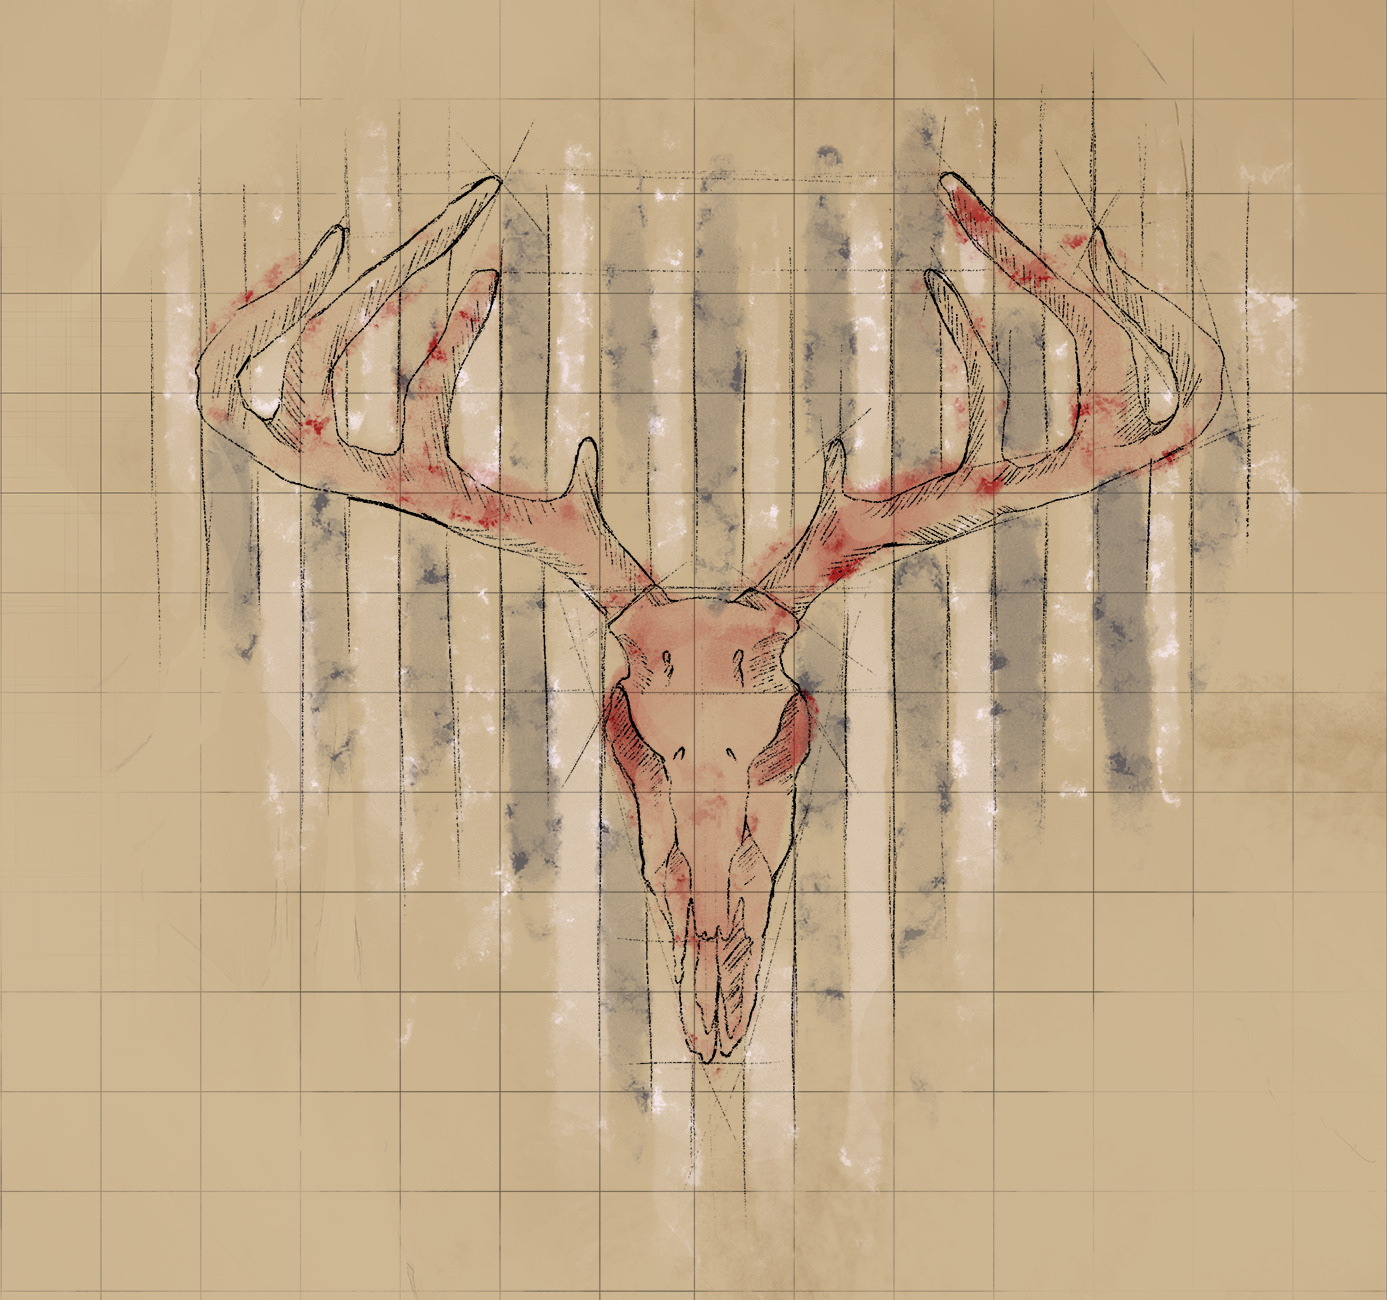
\includegraphics[width=0.9\linewidth]{media/norbury-huntersguildsm.png}
\end{figure}

The \emph{Hunter's Guild} is the slavery guild of \nameref{sec:Norbury}. It is
tasked with marking and handling new slaves, keeping track of existing ones,
and tracking down and returning those that have escaped. It operates an office
building and a large auction hall in the main square of the city. The hunter's
guild banner is a skull of a deer (with antlers) painted in red upon a white
background.

The guilds main income is the auction, and various administrative fees it
collects for transferring or freeing slaves. It does not charge for retrieving
runaway slaves, or for registering new slaves into the kingdom. The guild is
the main source of income for most soldiers of the Norbury army, as they pay a
share of the auction's profit for all soldiers who bring them new slaves to
sell. Many third party slavers or other slaving nations often trade goods with
the hunter's guild.

A lesser known duty of the Guild is to rescue Norbury citizens from slavery in
other slaving nations or city kingdoms. Although technically not bound by law
to do so, it often extends this service to any citizens of kingdoms that have
signed the \nameref{sec:Vonir Accord}. For these clandestine tasks it hires
special agents, spies and assassins whose rescue operations often bring them
in direct conflict with other slavers, such as the \nameref{sec:Velvet Hand}.

It also employs \emph{hunters}, often rangers, barbarians, fighters and
rogues, that are tasked with tracking down escaped slaves. These hunters are
allowed to enslave people, although they rarely do so. The guild has a
troubled past with enslaving citizens of other city kingdoms, and allied
nations, and has thus issued decrees for its hunters to go only after their
designated targets. These hunters have a reputation for being ruthless,
efficient, and exceptionally skilled professionals.

Although hunters make up a lion share of people employed by the guild, it also
hires bureaucrats, taskmasters, and wizards. These wizards are responsible for
developing the \nameref{sec:Slave Band} and the \hyperref[sec:Slave Mark]{slave
  runes}, arcane contraptions to bind and track slaves. The bureaucrats are
mostly responsible for tracking, organising, and categorising slaves, as well
as organising auctions and large scale trades. They are also responsible for
developing the colour code and classification system for slaves: \emph{White}
means that the slave is ``valueless'' or ``useless''. \emph{Gray} coloured
slaves have no special qualities or skills. \emph{Green} slaves have a special
skill that makes them valuable, which is often inscribed with a symbol right
next to the green identification mark. \emph{Red} slaves have no current
owner, and \emph{black} denotes slaves of high value. These are often
specialised craftsmen, priced fighters or perhaps slaves with magical
talents. Any of these colours may be combined with each other to easily signal
the current status of the slave.

The guilds mostly operates all across Aror, but mostly within the borders of
\nameref{sec:Norbury}, as well as the outlying baronies and smaller kingdoms,
and any nation or city kingdom that signed the \nameref{sec:Vonir Accord}. The
guild is banned from operating in city kingdoms and baronies that have banned
slavery, but still does so, often in secret.

\begin{35e}{Hunter's Guild}
  The Hunter's Guild is considered \emph{lawful evil}, and will hire anyone
  that has proven themselves reliable, mindful of the respective laws (such as
  the Vonir Accord), and is a skilled fighter, hunter, and tracker.
\end{35e}

% Magistrata Arcanum
\section{Magistrata Arcanum}
\label{sec:Magistrata Arcanum}
\label{sec:Mages Guild}

The Magistrata Arcanum, or simply the ``Mage's Guild'' in common parlance, is
the official arcane institution of \nameref{sec:Forsby}. It was founded in
\emph{GT:1332}, by the noble family of Lorham.

It operates a large tower within the city's centre, and is responsible for
operating the city's dragon teleporter, investigating arcane occurrences,
registering and keeping track of any arcane wielders within the city, as well
as constructing arcane equipment for the city's military. It gives out arcane
licences to anyone who wishes to practice arcane magic within the city walls.
Before the devil siege, the magistrata was allowed to research into all sorts
of magic, including necromancy, summoning and research into ancient evil
artefacts.

The guild is ruled by a council of high mages, who elect one of theirs to be
the prime representative, called the Arch Mage. The magistrata, in its long
standing history and tradition, has trained many great wizards, scholars,
and arcane researches, including Arch Mage \nameref{sec:Graham Balance} who
was one of its finest Arch Mages from \emph{GT:2120} to his death in
\emph{GT:2148}.

With its long standing history, the magistrata prides itself in its traditions,
and its expertise in all things arcane. Its mages are highly respected, and well
educated. Most of the guilds students are children of nobles, rich merchants or
of families with a long standing history of producing capable mages and wizards.
Thus the magistrata often has a reputation for being plagued with elitism,
nepotism, but is generally considered the second best mage's guild, after the
hall of knowledge of \nameref{sec:Fes al-Bashir}.

The magistrata has lost a lot of power, influence and reputation after the
\nameref{sec:Devil Siege} of Forsby. Many other powerful institution, and most
of the population put the blame on the siege on the guild, even though they
refuted any accusations. The nobility of Forsby and the church of
\nameref{sec:Lor} put heavy restrictions on the guild's operations, severely
limiting in what kind of arcane magic they are allowed to practise.

% Scions of Silence
\section{Scions of Silence}
\label{sec:Scions of Silence}

The Scions of Silence are a warrior order that still following the teachings
of the \nameref{sec:Silent Queen}. Their height of power was during the
\nameref{sec:Holy Crusade}, after which they waned in power and influence
with their goddess' demise. Still, small orders of the scions persist to
this day.

Their members must make a vow of silence, and many dedicated scions this to an
extreme and either cut out their tongues or sew their mouth shut to prevent
them from talking. They swear to obedience to the scion order itself, and
pledge before their now dead queen to protect the followers of the queen
against all and any threats. Since the followers of the queen have dwindled in
numbers, the scions have shifted their focus on destroying enemies of the
queen to take revenge on her death and betrayal.

Most Scions are now nothing but inquisitors that seek out and destroy any and
all followers of \nameref{sec:Aria}. Worshippers of Aria that are caught by
the scions are executed by fire, and their businesses and property are
destroyed. Since Aria worship is widespread in most city kingdoms and nations,
that often brings them in direct conflict with local authorities, and other
holy orders that seek to establish the rule of law.

During the era of the Silent Queen the Scions of Silence were once a respected
holy knight order, but have since fallen from grace and public knowledge. Then
they sought and harboured dangerous secrets, keeping them from being misused
or falling into the wrong hands. Their noble goals and reputation for being
incorruptible, steadfast and noble have since vanished. Now they are nothing
more than a violent cult that destroys and murders followers of Aria wherever
they can find them. The Scions recruit new young members through violence,
indoctrination and bind them to the order through fear, violence and
threats. Most members can no longer live in nations, baronies or city kingdoms
as their actions within the scions have made them wanted fugitives.

\begin{35e}{Scions of Silence}
  Few scions of silence still follow the old tenants and traditions of the order
  that would make them \emph{lawful neutral} as whole.

  Most follow the new teachings of betrayal and hatred toward followers of Aria,
  and are thus as a whole \emph{neutral evil}.
\end{35e}

% Silver Hand
\section{Silver Hand}
\label{sec:Silver Hand}

The \emph{Silver Hand}, a shadowy organisation found all around Aror, uses the
power of wealth to increase its influence all across the world. Their main goals
are to increase the individual wealth of its members, as well securing power,
influence and favours from powerful individuals to maintain their own standing
within society.

The organisation itself is secret, and so are its members. Only wealthy, and
powerful individuals are allowed to join, and must swear an oath to never
reveal or betray the organisation itself. Secrecy is upheld at all times, and
most of the times members do not know all other members of the society at any
given time. Members that join do swear to help each other, and to pool
resources against common threats and dangers.

The Silver Hand itself does not own any businesses, organisations or
influence, but their members do. Its members are often wealthy traders, crime
lords, or well connected politicians and nobles. Their members prefer to
operate covertly, plotting, stealing, spying and scheming in the background
over direct open involvement. Members of the organisation are very well
connected, and are capable of hiring any sort of service that would be
required to complete their objectives. They have connections to local
thieves', fighters' and assassins' guilds, as well as connections to corrupt
politicians and guards to remain in power. Members of the organisation meet
rarely, and always in complete secrecy. Often members arrive costumed or
disguised to avoid revealing their identities to others.

The organisation itself is centred around a select few individuals called
``beacons'' who know a limited subset of members called ``associates''. These
associates are often from the same kingdom or nation as the beacon. Beacons
also know one or two other beacons and can thus relay messages to other
branches of the silver hand. Messages, meetings, as well as combined
operations are organised through these beacons, who in turn relay these
messages and orders to their associates. This structure has allowed them
to compartmentalise their entire organisation, so that if one beacon or
associate is compromised the amount of information he could reveal is limited.
To get in contact with the Silver Hand, or to request aid from someone, a
member would contact his beacon, who in turn would further that request or
message throughout the organisation.

Individual members of the Silver Hand use the organisations power and
influence to eliminate competitors, gain unfair advantages in trade and
business, and avoid the repercussions and punishment of the law. The
organisation is known to spy, steal, murder and blackmail on all those
that might stand in its way.

Many members, and the organisation as a whole, is deeply connected to the
worship of \nameref{sec:Aria}, who sees the organisation as a logical
conclusion of her own teachings and dogmas.

\begin{35e}{Silver Hand}
  The organisation can be considered \emph{neutral evil}, and only accepts
  wealthy and powerful members.
\end{35e}

% Knight Order of Tavos
\section{Knight Order of Tavos}
\label{sec:Knight Order of Tavos}

The \emph{Holy Knight Order of Tavos} is one of the younger, but most
prestigious knight orders and fighter guilds on Aror. It was founded in GT:760
in Hraglund, and they follow the religious tenets laid down by a dwarven
matriarch \emph{Sir Tavos of Renfeld}, who received instructions to form the
knight order by \nameref{sec:Lor} himself. The knight order is always lead by
a patriarch or matriarch, who oversees the entire order from their headquarter
in \nameref{sec:Hraglund}.

Their banner is a stylised eagle, that spreads its wings downward toward the
ground, while a sun, representing Lor, rests overhead.

Although the knight order only accepts nobility as knights, they order demands
of them a monastic lifestyle. Members that join must forfeit their wealth and
earthly possessions, which are often donated to the poor and needy. The
Order's goals are to bring both law and Lor's light to its members, as well as
the world as a whole. Members must remain celibate, and follow a strict daily
routine meant to train their bodies, minds and will.

Knights and warriors of the Knight Order are also often tasked with protecting
the churches, priests, monasteries and pilgrims of Lor. As well as seeking out
and fighting creatures such as evil vampires, undead and daemons.

Members of the order are often paladins, knights, fighters, clerics as well as
rogues that wish to do good in the name of their patron god.  They can rely on
a tight network of churches, monasteries as well as outposts dedicated to
their god for support. Knights of the Order of Tavos are well liked and
received with most populations of the city kingdoms.

The church was also the instigator of many of the \nameref{sec:Crusades} Aror
has seen throughout its history.

However the knight order was directly involved in the \nameref{sec:Religious
  Civil War} in Norbury, which lead them from being exiled from the
kingdom. They also fought alongside the forces of \nameref{sec:Forsby} during
the devil siege, which made them ever more popular within that city.

\subsection{Relations}

By their very nature, and through the god they worship, they are often in
conflict with knights worshipping the \nameref{sec:Three Kings}, as well as
the five holy orders that follow the \hyperref[sec:Order]{Order Above Chaos}.
They often fight the former, while they are known to cooperate with the latter
should their goals align. The Knight Order is also banned from Norbury, and
\nameref{sec:Helmarnock} for several incidents with the local vampire and
umgeher population.

\begin{35e}{Knight Order of Tavos}
  The Order is considered \emph{lawful neutral}, and accepts knights, paladins,
  monks, fighters, rogues, clerics, duskblades as well as rangers. Their domains
  are strength, law, good and war, and their favoured weapon is the arming
  sword (``long sword'').
\end{35e}

% Ror-Aram Trading Corporation
\subsection{Ror-Aram Trading Corporation}
\label{sec:Ror-Aram Trading Corporation}

The \emph{Ror-Aram Trading Corporation} is the largest trading corporation on
Aror, headquartered in \nameref{sec:Fes al-Bashir}. It's wealth surpasses
that of most baronies, and even smaller kingdoms, and it operates a vast fleet
of both war- and trade ships.

It's main responsibility is to export the goods produced within Fes al-Bashir
to the other city kingdoms, but also import the products from other regions
into the kingdom. The companies success has made Fes al-Bashir one the richest
kingdoms, in which a wide variety of luxury goods (such as furs, spices and
precious stones) are common even among the middle class society. The company
has offices is all major city kingdoms, and tends to hold good relations with
these kingdoms.

However the company is also known for its predatory and unethical business
tactics, especially where it faces weaker opponents such as small native
tribes that happen to be on land of natural riches, smaller trading
corporations or even smaller villages and towns. The company openly trades
with slaves, often with the \nameref{sec:Velvet Hand} or the
\nameref{sec:Hunters Guild}. Although the company has its own fleet of war
ships, mostly to protect ships against pirates, it has also financed
privateers and pirates in the past to attack and weaken competitors.

The trading company also operates a bank, and is a main financier of
adventurers, expeditions, as well as survey teams looking for ancient ruins,
artefacts, natural resources, or new land. It mostly employs merchants,
traders, guards, entire crews for both its war, trading and privateer vessels,
as well as all sorts of people for expeditions and surveys.

A company of immense wealth and power, it holds vast political influence
within Fes al-Bashir and beyond. It keeps that power with its immense
wealth, but also by unethical means such as black mailing, sabotage and
espionage.

% Velvet Hand
\section{Velvet Hand}
\label{sec:Velvet Hand}

The \emph{Velvet Hand} is a slaver organisation that oversees the majority of
the slave trade within the kingdom of \nameref{sec:Fes al-Bashir}. The
organisation's banner is the Fes al-Bashir half moons in velvet colours upon a
white flag. The Hand is always lead by one leader, and a regime of under
bosses and corporals.

They are responsible for claiming, registering and selling most of the slaves
within the kingdom, much like their Norbury counterpart the
\nameref{sec:Hunters Guild}. They often work closely together with the
\nameref{sec:Ror-Aram Trading Corporation} to sell, buy and hunt for their
goods outside of the kingdom.

Unlike the more sophisticated arcane tactics of Norbury, the Velvet Hand still
relies on branding behind the ears to mark slaves and their respective
owners. However do have copied the colour coding of slaves from the Hunter's
Guild in recent years.

The Velvet Hand is bound to the \nameref{sec:Vonir Accord}, and may thus not
enslave citizens of signing nations. Even though it is technically illegal,
they are known to break the accord regularly, and are thus notorious and even
feared all across the world of Aror. The Velvet hand also employs slavers that
actively seek new merchandise to sell back to the city. Their slavers often
roam the land with caravans, or the high seas with ships and prey on any they
perceive as potential new merchandise. This often brings them in direct
conflict with other city kingdoms or powerful organisations. The Hand manages
to stay out of these diplomatic incidents by allowing third party slavers act
without their knowledge and with plausible deniability.

The Velvet Hand often hires anyone willing to become slavers, and cares very
little on how their slaves are acquired. Velvet Hand slavers are notoriously
feared and despised all across the world, but the Hand remains a powerful,
rich and well connected organisation that is not easily unseated from their
place of power.

\begin{35e}{Velvet Hand}
  All in all the Velvet Hand is considered \emph{neutral evil}, and will hire
  any adventurer that is willing to do business with them. They operate like
  a criminal business venture, and are mostly interested in profit.
\end{35e}

% Wayfaerer's Guild
\section{Wayfaerer's Guild}
\label{sec:Wayfaerers Guild}

The Wayfaerer's Guild (``Wayfaerer'', ancient teranim for ``children of
\hyperref[sec:Eigyr]{Way}'') is the original hunting and adventurer guild that
was instrumental in founding of \nameref{sec:Hraglund}. Their members are
prolific hunters of all kind (such as warriors, rangers and wielders of
magic), that price themselves with being able to hunt and kill all wild and
dangerous beasts that may threaten civilisation.

The guild flies a green banner with a white shield, depicting a five headed
hydra. This is the same banner that is also used by the kingdom of Hraglund,
which sometimes causes confusions.

Members of the guild can be hired by anyone who need a dangerous beast or animal
taken down. It deploys many capable trackers, hunters, as well as fighters,
mages and scholars trained to defeat dangerous creatures such as undead, demons,
vampires, lycanthropes or even dragons. Although the guild itself is rather
small, and mostly centred around Hraglund and the outlying reaches, it can boast
with a century long tradition and track record.

Hunters of the guild may not hunt for sport, but instead must swear an oath to
only hunt and kill those creatures that would endanger others or the innocent.
Although they are allowed to hunt sentient creatures (such as evil undead, or
lycanthropes), they may not pursue sentient creatures without express permission
of the local law enforcement. The guild has a favourable reputation across all
of Aror, and are often called from remote corners to aid in the hunt of the
most dangerous of game.

The guild itself has several smaller outposts and save houses strewn across the
world for members to use, and will give any member the means to hunt and kill
whatever dangerous game they are after. It provides spell crafting services,
such as divination spells to track down prey, weapons, armours, healing, as well
as lore and knowledge on a variety of subjects. Hunters of the guild earn well,
and will have their families supported should they die during a hunt.

Although small, the guild earns well from the bounties it collects and the fees
it charges for its services. The nobility of \nameref{sec:Hraglund} also bestows
their patronage toward the guild, as an eternal thank you for their services
during the foundation of the city itself.

\begin{35e}{Wayfaerer's Guild}
  All in all the dogma of the Wayfaerer's guild should be considered
  \emph{chaotic good}. They accept anyone who has proven himself as a capable
  hunter and tracker, especially fighters, wizards, rangers, barbarians and
  rogues.
\end{35e}



% Chapter 6: Planes & Planets
\chapter{Planes \& Planets}
\label{sec:Planes}

Around 800.000 years ago, when the dragons first settled Aror, they
deliberately cut off the planet from all other planes of existence. Thus no
plane could ever contaminate the ``material plane'' (i.e. Aror) ever
again. The dragons never gave a reason on why they did so, but most scholars
agree, it was an attempt to monopolise planar travel, and thus lock out their
enemy the \nameref{sec:Giants}.

Roughly 200.000 years later the giants managed to breach the blockade, and
invaded Aror. After they were defeated by the dragons, the blockade was
reinforced and held until \emph{MI:1918}, or over 600.000 years. The breach
was sealed again, with the help of the wizards of the \nameref{sec:Magistrata
Arcanum}, and the \nameref{sec:Hall of Knowledge}.

No plane of existence can be reached directly from Aror, and Aror cannot be
directly reached from any other plane of existence. However planets near Aror
within the galaxy can be reached through teleportation spells. Some of these
planets support life, and from them you could reach other planes of existence.
Due to the difficulty of reaching other planes from Aror, inter-planar travel
is rather rare. What is quite common however, are visits to the planets that
are close to Aror, such as \nameref{sec:Aurelis}.

Since there is no astral plane reachable from Aror, the souls of the dead
instead go into the \nameref{sec:Soul Well}. There are also no astral beings
that are worshipped as gods on Aror, since the followers would not be able to
communicate with it. Most scholars, wizards and leaders of Aror agree that
this isolation from the planes is a good thing, as there already are a
plethora of threats native to Aror. However this also means that many
extra-planar threats (such as the Githyanki) are unknown to people of Aror.
The mechanics that lead to planar isolation have even been copied by other
races, such as the \nameref{sec:Devils}, or the \nameref{sec:Aurelis} to
shield their realm from other planes.

The most confusing part about planar and planetary science on Aror is the
terminology. Since very, very few have actually travelled to another plane,
the distinction between the two concepts is not well known. The words
``planes'' and ``planet'' are used interchangeability, causing confusion to
those that know the difference.

\aren{This mistake was sadly also made repeatedly by our esteemed Graham, and
for the sake of preserving the original work, these errors are retained.}

\section{Planets}

% Celestis
\subsection{Celestis}
\label{sec:Celestis}

The planet of ``Celestis'' is the closest inhabited planet to Aror. It is the
home of the \nameref{sec:Aurelis}, a species of winged humanoids that have
generally been seen as allies by the people of Aror. It is the third planet
from its sun, which is confusingly also called Celestis.

Before the planets devastation, it was not unlike to Aror itself. It had two
snowy, cold polar regions to the north and south; lush rain forests and tropical
regions near the equator, as well as high mountain ranges and boreal forests.
The vast majority of the planets surface is covered with water, but it has one
massive continent that harbours all of the land-based live. The southern part
of the continent housed most of the Aurelis, while a minority of the Aurelis
lived in the northern part of the continent. The planets biggest city, and
capital for the Aurelis, called ``Gamos'' is located in the southern
hemisphere of the planet.

The planet was heavily devastated during an event called the \nameref{sec:War
in Heaven}. The \nameref{sec:Scourge} of the \nameref{sec:Abyss} managed to
infiltrate and settle on the northern part of planet, leading to a century
long conflict that devastated more than half of the land based life on the
planet. The scourge consumed most of the native land-based flora and fauna,
draining most land locked salt-water seas, lakes and rivers of the northern
hemisphere. While the scourge mostly consumed the north, leaving it a barren
and deserted wasteland, the south, and especially the land around Gamos
remained untouched. Most Aurelis from the north fled towards the capital,
settling the surrounding land by building villages, towns and cities.

The devastation of the planet's plant and animal life was so devastating, that
it lead to a shift in the planets overall climate towards hotter summers,
milder winters, and overall less rainfall. The remaining Aurelis struggle to
resettle the vast desert of the northern hemisphere, not only to restore the
previous beauty, and ecological diversity, but also to gain more land for
farming. This process has been slowly progressing for over eight millennia,
continuously threatened by the resurgence of small growths of the
\nameref{sec:Scourge} trapped in the desert, as well as new races arriving in
the desert. \nameref{sec:Gnolls} from Aror, as well as \nameref{sec:Giants}
have made the northern wasteland their home, and are contesting ownership of
the land from the Aurelis.

After the incursion of the scourge, the sages and wizards of Gamos have copied
the arcane technology from the dragons that blocks inter-planar travel. Although
isolation slowed the recovery of the people, and the planet, the risk of
another scourge invasion was deemed to high. Celestis can still be visited by
teleporting across the vast inter-stellar expanse, but it can no longer be
visited through planar shifts.

Nevertheless the planet remains habitable, and after defeating the Scourge
millennia ago, both the planet and its people are recovering. Especially Gamos
is often visited by Arorian traders, and diplomats, as many city kingdoms see
the Aurelis as their partners, or even allies.



% Chapter 7: Classes & PrC
\chapter{Base and Prestige Classes}
\label{sec:Classes}

An overview on how most professions and specialisations are perceived in the
world of Aror. If you are a inter-planar traveller visiting us, you should
read this article very carefully. Some professions, especially some divine
and arcane wielders might otherwise find themselves at the wrong end of an
inquisitions.

% Base Classes
\section{Base Classes}
\label{sec:Base Classes}

\subsection{Barbarian}
\label{sec:Barbarian}

Most barbarians can be found among the more savage tribes of
\nameref{sec:Iafandir}, \nameref{sec:Dirgewood} as well as the Toralian
heights. Barbarians there are an integral part of many smaller tribes, being
warlords, warriors, hunters and chieftains. Many barbarians follow the example
of \nameref{sec:Eigyr}, the mighty huntress, who is often seen as a positive
example on how a mighty warrior shall serve his community and the greater
good. Her deeds inspire young warriors of any race, background, gender or
religion to achieve ever great feats and heroics. Unlike other worlds, there
are no tribes solely made up of barbarians, instead these mighty warriors are
always embedded in existing villages and tribes.

The monstrous races also favour the reckless yet courageous style of battle
the barbarians do, often following the example set by \nameref{sec:Three Kings}.
These warriors are often called ``beast warriors'' or ``ravagers'', particularly
known for their savagery and unparalleled strength in battle.

\subsection{Bards}
\label{sec:Bards}

Bards can be found in all across Aror, in a variety of roles, shapes and
professions. Many artists, musicians, actors and performers of
\nameref{sec:Avenfjord} are bards, enticing large crowds with their artistic
skill and enchanting performances. But bards can also be found among the
\nameref{sec:Old Ways}, either telling or performing plays about the stories
so deeply entrenched within that religion. Many rituals of the old ways
include chanting and music, and so many shamans and spiritual leaders of
communities that follow the old way are bards.

\subsection{Clerics}
\label{sec:Clerics}

Clerics, priests, child of the gods, acolytes, shamans, and many witches are
all the same: followers of either the true or lesser gods. They highly valued,
if not the most important, member of any civilisation. They share the wisdom,
and power of their gods with their community, and lead them through spiritual
crisis and hardship. Clerics take on my roles, often depending on the
spiritual journey their god or deities has put them on. Some are healers, some
are torturers. Some guide their flock towards peace, love and understanding,
while others chant their message of hatred, war and destruction to drive their
communities towards hostility against others.

\subsection{Druids}
\label{sec:Druids}

The druids where once the spiritual leaders of the old ways, but are now a
community facing imminent extinction. Druids split from the shamans and priests
of the old ways, by abandoning the worship of the holy mothers, and instead
worshipping \nameref{sec:Daemons}, in particular \nameref{sec:Leszy} and the
\nameref{sec:Percht}. A few druidic circles, including the ``Circle of
Rebirth'' remained loyal the holy mothers, and continued to worship
\nameref{sec:Morana}, which ultimately, also lead them fall from grace in the
eyes of the followers of the old ways. Although many druidic circles followed
practices and traditions inspired by their often evil deities, their lives
deep within forests and marshes of the \nameref{sec:Dirgewood} and Toralian
Heights isolated them from other humanoid civilisations. They were seen as
religious fanatics, albeit few in numbers and generally considered harmless.

This all changed during the age of battle against the beast races, when both
the humanoid races, and the intelligent beast races, attempted to outbid each
other in a rush for resources and industrial growth. Forests were cut down,
marshes drained, lakes fishes dry, and lush grassland burnt down to make way
for farmland. This enraged both humanoid and beast race druids, causing them
to solidify in their religious fanaticism. They began to work together to
keep both humanoids and beasts out of their forests, often devising evil,
sadistic and cruel means with the help of their equally deranged deities.

Druids are the sole reason \nameref{sec:Fey} and \nameref{sec:Lycanthropes}
exist, and terrorise the humanoid and beast population to this day. Many
druids were not above acts of domestic terrorism against large baronies and
kingdoms, poisoning wells and food stores, turning populations against their
will into fey, causing farmland to wither and die, and abducting the young to
bolster their own numbers. In turn, druids were hunted to near extinction.

Those few that remain, hide in the depths of the forest or marshes and hold on
to their believes and fanaticism. These remaining circles are the aforementioned
``Circle of Rebirth'', ``Nightowls'' and ``Ondtrad''. The ``divine'' magic they
wield stems from the daemons they worship, and continues to poison them and all
they create. Those druids that escape from the clutches of these fanatic cults
find they are still not welcome among either their humanoid or monstrous
brethren. Any appearance and terror from fey is blamed on them, as are any
failings in the harvest. Knowledge about the history of druids, and their
misdeeds are common, as they are often used as a boogeyman to frighten
children away from forests. Almost all city kingdoms and baronies ban druidic
worship of the daemons, and will arrest, exile or even execute druids.

\graham{If you are a druid attempting to flee your cult and join a modern
  civilisation, know this: Unless you lie about your heritage, you might be
  welcomed with aversion and hostility.
}

\begin{35e}{Druids}
  Druids on Aror have a predisposition towards being evil against their
  civilised brethren. As always, not all are evil, and many do not have a
  choice as the very daemons they worship poison their minds and judgements.
  Knowledge about who and what druids are, and what they have done in the
  past is wide spread among most people and monstrous races on Aror.
\end{35e}

\subsection{Fighter}
\label{sec:Fighter}

The backbone of any and all civilisation. If you can defend your family, your
land, your king and your country you will be welcomed anywhere. Fighter,
warriors, archers, two-handed wielding Landsknechte, mercenaries, shield
maidens, master fencers or ruthless thugs are but a few of the multiple
facets that these brave men and women play in your society.

\aren{There is inherent strength in being able to wield a weapon effectively.
  Limiting yourself by preconceptions on their inferiority against magic,
  makes you much, much weaker than you are.
}

\begin{note}
  You should consider giving Fighters more skill points.
\end{note}

\subsection{Monk}
\label{sec:Monk}

Monks are rather uncommon to the world of Aror, as in, not many have actually
met or even seen a monk. Almost all of the warrior monks study their art in
solitude, or join monastic organisations such as the \nameref{sec:Fifth Order}.
Although often monks follow a strict traditional life of order, mental training
and disciple, it is not required to learn the martial arts.

\begin{35e}{Monk}
  Monks no longer have any alignment restrictions, and the longsword, rapier,
  spear, bows (of any form), kuhkri and scimitar are added to the list of monk
  weapons.
\end{35e}

\begin{note}
  See the monk more as a warrior who learns and practices martial arts on a
  spiritual level. This can include ``western style'' martial arts, which are
  often referred to as ``HEMA''. On Aror a monk is no longer strictly
  ``eastern'' martial arts, especially since the 3.5e monk was a very poor
  representation of that in the first place.
\end{note}

\subsection{Paladin}
\label{sec:Paladin}

Those that you might know and call ``paladin'' and might see as holy avengers
and servant of the gods, are just a small subset of the wide variety of
fighters, warriors and that gain divine power through servitude. All of them
have one theme in common: a strongly held set of believes, and the willingness
to fight those that would oppose said believes. While the classical, almost
stereotypical, holy crusader that follows \nameref{sec:Lor} or
\nameref{sec:Order}, who wears heavy plate armour and smites evil foes do
exist, and might even be the majority, they are not the only servants that are
granted divine power.

\nameref{sec:Marwaid} sees servitude as a form of sacrifice to be held
precious, holy and divine even if the servitude is not to a god or church. Many
paladins work for the ideals represented by factions, organisations, their own
set of believes, serve powerful individuals in a \nameref{sec:Life Bond}, or
even long lost, and dead gods. All of these are actually following the ideals
of Marwaid and are thus granted divine power.

\begin{35e}{Paladin}
  There are no longer any alignment restrictions on paladins, and you no longer
  have to directly serve a deity to be a paladin. The mere act of acknowledging
  strength through servitude (to a person, ideal, church, organisation etc.) is
  seen as honourable to Marwaid and thus makes you eligible to be a paladin,
  regardless of alignment.

  Classical 3.5e paladins can choose the Order, Lor, Marwaid, devils or
  daemons (among others) as their patron deities.
\end{35e}

\subsection{Sorcerer}
\label{sec:Sorcerer}

Sorcerers, as they are called by the arcane institutions, are people that wield
arcane magic without formal training. They often lack formal arcane training,
and simply just ``do it''. Many sorcerers are part of tribal societies,
villages, or cities in rural areas, where they are often called ``shaman'' or
``witch'', and offer their services towards the community. Although many wizards
look down on these free spirits, their power is undeniable.

\graham{Never look down on a witch, or she just might hex you.}

\subsection{Ranger}
\label{sec:Ranger}

Rangers are people of the forest, the swamp or the mountains. They are either
defenders of nature, hunters, but above all else, followers of the
\nameref{sec:Old Ways} that live in harmony with the teachings of the old
mothers, nature, and their people. In many tribes, villages and cities rangers
are a cornerstone of the community, often serving as a link between the people
and nature. Some wayward rangers also live in the city kingdoms, often serving
as hunters, trackers, priests, and in some rare cases, as slave hunters and
soldiers.

\aren{Rangers are most typically spiritual leaders of smaller tribes and
  villagers, and might often bear titles such as ``priestess'', ``shaman'' or
  ``elder''.
}

\subsection{Rogue}
\label{sec:Rogue}

Rogues are as multi faceted in their occupation within as their skills. Some
are spies, thieves, burglars, diplomats, crime lords, pirates or smugglers.
But most of them lead some sort shady life at the edge of legality. They are
so ubiquitous, that is hard to say where to start looking for one.

\graham{Perhaps among the authors of this book.}

\subsection{Warlocks}
\label{sec:Warlocks}

Warlocks have made a pact with a powerful entity in exchange for power. The
basic premise of these pacts is that the power helps the warlock grow in
power and strength, and once the warlock dies his empowered soul is already
promised the powerful entity. The powers that warlocks wield were invented
by \nameref{sec:Forneus}, and thus many of his disciples (be they infernal
or from Aror) follow him. The devils are not the only ones that grant powers
such as these to their disciples. Many \nameref{sec:Daemons} have started
to foster their own disciples.

No warlock is particularly welcomed on Aror, as resentment towards devil
worshippers has increased after the devil siege against Forsby. Especially if
you also have infernal traits, or are a \hyperref[sec:Tieflings]{tiefling},
the authors advise keeping your powers secret, and your appearance hidden
behind illusion.

\subsection{Wizards}
\label{sec:Wizards}

Wizards are the rare view that have shown both talent and dedication to study
the arcane arts. Albeit wizards are extra-ordinarily rare on Aror (very few
have the mental capacity to understand, and wield the logic required to cast
spells), they are highly regarded in almost all nations and regions. Wizards
make up most of the high elite that rule \nameref{sec:Fes al-Bashir} through
the Hall of Knowledge, they study the arcane arts in the \nameref{sec:Magistrata
  Arcanum}, craft and create wondrous machines in \nameref{sec:Stenheim} and
scry the northern sea of \nameref{sec:Norbury} for immediate raids.

Very few wizards ever reach the pinnacle of their power, as natural death
takes them before they could unlock their higher mysteries of arcane
knowledge. Those that reach these unfathomable heights of arcane power are
granted the title ``Grand Magus'' by the \nameref{sec:Hall of Knowledge},
of which none have ever surpassed the power of \nameref{sec:Graham Balance}.

In recent years the both the Hall of Knowledge and the Magistrata Arcanum
have confirmed that \nameref{sec:Taras} has achieved the same power as a
Grand Magus, but both institutions have denied him that title.

\begin{note}
  High level wizards (>15) are extra-ordinarily rare on Aror, with only a few
  living at any given time. Graham Balance was the most powerful wizard ever
  known to live (level 19), with Taras coming in close second (level 17).

  Most wizards are around level 5 or 9, with a few select leaders and professors
  of arcane institutions reaching level 10 to 14. The title of ``Grand Magus''
  is bestowed upon anyone who can proof that they can cast level nine spells.
\end{note}



% Chapter 8: Characteristics
\chapter{Heroic Characteristics}
\label{sec:Heroic Characteristics}

% Skills
\section{Skills}
\label{sec:Skills}

A few skills have new uses, and some additional rules apply to them in
\emph{Everblack}.

\subsection{Knowledge}
\label{sec:Knowledge}

The knowledge family of skills have two new entries: \emph{Knowledge (Old Ways)}
and \emph{Knowledge (Soul Magic)}.

\emph{Knowledge (Old Ways)} encompasses the knowledge about rituals, practices,
believes and customs of the religion of the \nameref{sec:Old Ways}. It mixes
knowledge about the religion itself, as well as parts of soul magic, which are
presented in that religion in the form of ancient rituals and incantations.

\emph{Knowledge (Soul Magic)} functions much like \emph{Knowledge (Arcana)}
except for spells, magic and creatures related to soul magic.

\subsection{Speak Language}
\label{sec:Speak Language}

The common languages of \emph{Everblack} are summarized in the following
\hyperref[tbl:Languages]{table}.

\begin{table*}[!htb]
  \captionsetup{labelformat=empty,font={large,bf},position=top}
  \caption{Languages of Aror} \label{tbl:Languages}
  \rowcolors{1}{white}{light-grey}
  \begin{tabular}{l p{8cm} l}
    \textbf{Language} & \textbf{Typical Speakers} & \textbf{Alphabet} \\
    Ancient Teranim & \nameref{sec:Tynrikke}      & Ancient Teranim \\
    Doresh          & Deep races, such as \nameref{sec:Deepkin} & Old Teranim \\
    Draconic        & Dragons, mages and scholars & Draconic, Teranim \\
    Druidic         & Druids (secret language)    & Ancient Teranim \\
    Enro'ad         & Elves, Halflings            & Taavid \\
    Goblin          & Goblins, Bugbears           & Taavid \\
    Giant           & Giants, ogres, trolls       & Giant \\
    Gnoll           & Gnolls                      & Gnoll \\
    Inua            & \nameref{sec:Inua}          & Inua \\
    Kalest          & People of \nameref{sec:Arania} & Teranim \\
    Old Teranim     & People of the \nameref{sec:Dirgewood} and by followers of the \nameref{sec:Old Ways} & Old Teranim \\
    Orcish          & Orcs                        & Taavid \\
    Reatham         & People of \nameref{sec:Forsby} & Teranim \\
    Rutari          & Dwarves                     & Rutari \\
    Senari          & Fey                         & - \\
    Taavid          & Halflings                   & Taavid \\
    Teranim         & Humans, Halflings, Elves    & Teranim \\
    Tolarn          & Hobgoblins                  & Taavid \\
  \end{tabular}
\end{table*}

\subsection{Forgery}
\label{sec:Forgery}

Anyone who can cast \emph{Arcane Mark}, can attempt to forge a
\hyperref[sec:Citizen Mark]{citizen mark} or a \hyperref[sec:Slave Mark]{slave
mark} using the \emph{Forgery} skill while casting the spell. This special
use of forgery and the spell stretches the casting time to ten minutes. The
character takes the \emph{Forgery} check as normal, taking a -10 penalty on
the check. The same procedure can also be used to forge \hyperref[sec:Nobility
Mark]{nobility marks} but the \emph{Forgery} check incurs an additional -10
penalty, for a total of a -20 penalty on the skill check.

\subsection{Open Lock}
\label{sec:Open Lock}

Anyone who can also use the skill \emph{Spellcraft} can attempt to remove
a \nameref{sec:Slave Band} from a slave by using the \emph{Open Lock} skill.
This attempt requires a basic arcane lab, arcane ingredients worth fifty
shards which are consumed in the process, and takes one our to perform.
The DC of the \emph{Open Lock} and \emph{Spellcraft} is the caster level
of the slave band plus 30.

\FloatBarrier

% Feats
\section{Feats}
\label{sec:Feats}

\begin{table*}[!htb]
  \small
  \captionsetup{labelformat=empty,font={large,bf},position=top}
  \caption{Overview of Feats}
  \rowcolors{1}{white}{light-grey}
  \begin{tabular}{l p{4.5cm} p{7cm}}
    \textbf{General Feats}        & \textbf{Prerequisites}           & \textbf{Benefit} \\
    Improved Weapon Finesse       & Weapon Finesse                   & Gain dexterity on damage with finesse weapons \\
    Craft Implant                 & Caster level 3rd                 & Craft implants \\
    Greater Weapon Specialisation & Proficiency with weapon, Greater Weapon Focus with weapon, Weapon focus with weapon, Weapon specialisation with weapon, BAB 12 & +2 bonus to damage rolls with weapon, and doubled damage die with weapon for 12th level Fighters \\
    Radiant Soul                  & Soul Awakened, 13+ Charisma      & Your soul power point die step increases by one \\
    Weapon Specialisation         & Proficiency with Weapon, Weapon Focus with weapon, BAB 4 & +2 damage with selected weapon, and bigger damage die as a 4th level Fighter \\
  \end{tabular}
\end{table*}

\subsection{General Feats}
\label{sec:General Feats}

\begin{35efeat}{Craft Implant}
  \srditem{Description}{You can craft small magical implants that can be
    inserted into a creature's body. These implants then grant special or
    extraordinary abilities, or even spell like abilities. Crafting an implant
    takes one day for each 1000 g the implant costs, and you must spend $
    \frac{1}{25} $ of the implants gold cost in XP, and use up raw materials
    half of this GP cost.

    You can also mend a broken implant, which costs half the gold, XP, time
    and materials of what it would cost to create the item anew from scratch.

    An implant is created for a special creature type in mind and will only
    work for said creature. But for half the cost in gold, XP, time and
    materials of what it would cost new, you can adapt an existing implant
    for another creature type.

    Some implants incur extra costs in material components or XP, as noted in
    their descriptions. These costs are in addition to those derived from the
    item's base price. You must pay such a cost to create an item or to mend a
    broken one.
  }
  \srditem{Prerequisite}{Caster level 3rd}
\end{35efeat}

\begin{35efeat}{Greater Weapon Specialisation}
  Choose one type of weapon for which you have already selected Weapon
  Specialisation. You can also choose unarmed strike or grapple as your weapon
  for purposes of this feat.

  \srditem{Prerequisites}{Proficiency with selected weapon, Greater Weapon
    Focus with selected weapon, Weapon Focus with selected weapon, Weapon
    Specialisation with selected weapon, BAB 12
  }
  \srditem{Benefit}{You gain a +2 bonus on all damage rolls you make using the
    selected weapon. This bonus stacks with other bonuses on damage rolls,
    including the one from Weapon Specialisation (see below). If you are a
    12th level Fighter (or higher), then the amount of damage die are doubled
    for the given weapon.
  }
  \srditem{Special}{You can gain Greater Weapon Specialisation multiple
    times. Its effects do not stack. Each time you take the feat, it applies to
    a new type of weapon.

    A fighter may select Greater Weapon Specialisation as one of his fighter
    bonus feats.
  }
\end{35efeat}

\begin{35efeat}{Improved Weapon Finesse}
  \srditem{Description}{You can add your dexterity modifier instead of your
    strength modifier to damage for weapons that can be used with Weapon
    Finesse}
  \srditem{Requirements}{Weapon Finesse, Bab 6, Dexterity 17}
\end{35efeat}

\begin{35efeat}{Radiant Soul}
  \srditem{Description}{Your soul power point die step is increased by one,
    for any future class levels, as long as they give you soul power points.
  }
  \srditem{Requirements}{Soul Awakening, 13+ Charisma}
\end{35efeat}

\begin{35e}{Weapon Specialisation}
  Chose one type of weapon for which you already have selected the
  \emph{Weapon Focus} feat. You can also choose unarmed strike, or
  grapple as your weapon for purposes of this feat. You deal extra
  damage when using this weapon.

  \srditem{Prerequisites}{Proficiency with the selected weapon, \emph{Weapon
      Focus} with selected weapon, BAB 4
  }
  \srditem{Benefit}{You gain a +2 bonus on all damage rolls you make using the
    selected weapon. If you are a 4th level Fighter (or higher), the selected
    weapon also has its damage die increased by one step when you use it.
  }
  \srditem{Special}{You can gain this feat multiple times. Its effects do not
    stack. Each time you take the feat, it applies to a new type of weapon.

    A fighter may select Weapon Specialisation as one of his fighter bonus
    feats.
  }
\end{35e}



% Chapter 9: Magic
\chapter{Magic in Everblack}
\label{sec:Magic}

Magic is ever present in the world of Everblack. It is used by scholars and
wizards, to improve the lives of everyone, or by dark and ruthless mages to
bring harm and war upon the world. This chapter discusses the foundations of
magic within the world of Everblack, and brings new rules for magical effects
such as \emph{rituals} and \emph{soul magic}.

\section{Three Sources of Magic}

There are three main sources of magic in the world of Everblack. Both divine
and arcane magic, which stem from the same source. The distinction is that
divine magic is granted already prepared in the form of spells to divine
casters, while arcane researchers and scholars build their own spells out of
that same raw magical energy that also fuels divine spells.

The second power are psionical powers, which manifest in the powerful minds of
psykers, and psionic creatures such as \nameref{sec:Ilians}. They do not draw
their power from the same pool as divine or arcane power, and come directly
from the mind of the powerful being that casts that spell. Compared to the
other two, psionic powers are the rarest on Aror.

The third magical source of power is the soul of living beings, which allows
one to cast \nameref{sec:Soul Magic}. This power is either drawn from one's
own soul, or from souls of those around them. Much like psionic power, it
stems directly from the trained or inherent power of the individual, and does
not rely on external sources, such as a raw energy web that seeps in from
other planes. While arcane or divine necromancy is the art of manipulating
and corrupting bodies, soul magic is the art and craft of using ones inherent
power to shape and fuel souls.

\subsection{Divine Magic}
\label{sec:Divine Magic}

Divine Magic comes directly from a deity, a deity representing a concept, or a
powerful individual, such as \nameref{sec:Daemons} or \nameref{sec:Devils}. In
the case of lesser deities, the deity in question grants that power, in the
understanding that the power is used to further the deities interests, and
goals. Once that power is granted, it cannot be revoked by the lesser deity
until it is used, or lost. True deities do not exist as living beings, being
concepts given power, and thus work differently. A priest that follows a true
deity draws strength and power from the concept said deity represents. For
example a priest of the \nameref{sec:Order} draws strength from an inner desire
to create order out of chaos, and from defeating the evil that may stem from
chaos. A priest of a true deity may lose their power should they stray too
far from their true deities concepts, ideas and ideology.

\subsubsection{Resurrection}

Resurrection magic works differently on Aror. Upon death all souls dilute into
the soul well, coming apart by the seams until they can no longer be recovered.
Much like you cannot recover the exact same water particles once you have
poured them into the ocean. The soul of a recently deceased can only survive
this dissolution of the self if another powerful soul of the well intervenes.
While some powerful souls may do so to further their own reasons, many will only
do so if they see a benefit for themselves. So those that wish to cheat death
will have to make a deal with a powerful daemon.

\begin{35e}{Resurrection}
  Any resurrection or reincarnation magic only works within 1d4 hours of
  death. After that resurrection magic only succeeds if a powerful daemon
  wishes for it to succeed.
\end{35e}

\subsection{Arcane Magic}
\label{sec:Arcane Magic}

Those deities that give power to their clerics, and priests cannot do so with
perfect efficiency. The process of granting, and using divine powers leaks
magical energy which remains trapped on Aror. This magical energy can be
harvested, shaped, and channelled into spells by those that study the craft of
\emph{arcane magic}. Due to its versatile nature, and its inherent
independence from a higher power, arcane magic is considered more powerful
that divine magic but also exceptionally difficult to study, hard to
understand, and dangerous to wield.

\begin{35e}{Arcane Magic}
  Arcane Magic of \emph{all} forms require years to learn, and wield even at
  the most basic levels. Any and all arcane wielders (even those that use
  ``inherent'' arcane magic like bards and sorcerers) are usually 10 to 20
  years older their divine or martial counterparts to make up for the years
  spent training, and learning. Unless of course they one of the rare
  \hyperref[sec:Graham Balance]{child prodigies}.
\end{35e}

\subsection{Summoning}
\label{sec:Summoning}

The \emph{summoning} and \emph{calling} sub schools of arcane magic are
related with bringing extra-planar creatures to or from Aror. Due to the
existence of a device called the \nameref{sec:Monolith} these sub schools of
magic are harder to perform and practice than other schools of magic. Since
summoning devils, or even \nameref{sec:Demons} is incredibly dangerous, many
cities ban these schools of magic in their entirety.

Any extra planar creature summoned to Aror will fade away to the soul well
just like any other living being residing on Aror. This has made Aror a very
unpopular destination for many more powerful extra-planar species, as they
will not be sent home upon defeat, but risk permanent death at the hands of
the soul well. Further details about how this affects summoning magic can
be found in the book's section about the \nameref{sec:Monolith}.

\subsection{Necromancy}
\label{sec:Necromancy}

Necromancy is the art and craft of manipulating both body and soul to achieve
a purpose. In many cases the craft destroys the soul, leaving only a soulless
husk behind, while in others it does exactly the reverse. The art of
necromancy was discovered when \nameref{sec:Morana} turned some of her
followers to vampires, and has since been excessively studied by scholars,
priests and wizards. \nameref{sec:Isamir} also gave the power of necromancy to
the \nameref{sec:Inua} who closely guard the secrets of their rituals, spells
and incantations.

Liches, and \nameref{sec:Vampires} are the epitome of applied necromancy, and
many scholars have spent millennia studying them to better understand the
craft. While many necromancers wish only to study the vampire to better help
them survive, much like a doctor would for the living, others use the powers to
do evil, creating vicious and horrid creatures to do their bidding. Necromancy
is thus outlawed in many regions, and cities, requires oversight, or a special
permit.

% Rituals
\section{Rituals}
\label{sec:Rituals}

Rituals, or incantations, are powerful \emph{soul magic} or \emph{divine}
rituals can be cast by anyone, even those that are not arcane or divine
casters. These rituals often require specific words to be chanted, ritual
places specifically crafted and arranged for the incantation, often take
several hours of preparation and then to perform, and often require more than
person to be successfully performed.

The most prominent source of rituals are the lore and history of the
\nameref{sec:Old Ways}, as well as the lore of druidic circles. While the old
ways use rituals to heal, the druids use them for nefarious purposes, such as
cursing enemies with \hyperref[sec:True Lycanthropes]{true lycanthropy}.

\begin{35e}{Rituals}
  See the Unearthed Arcana variant magic rules on \emph{Incantations} on how
  to perform soul magic rituals.
\end{35e}

% Bone to Bone and Flesh to Flesh
\subsection{Bone to Bone}
\label{sec:Bone to Bone}

\songquote{Merserburger Zaubersprüche}{
  sôse bênrenki, sôse bluotrenki, sôse lidirenki: \\
  bên zi bêna, bluot zi bluoda, \\
  lid zi geliden, sôse gelîmida sîn.
}

\emph{Bone to Bone} is an ancient healing ritual performed by the followers of
the \nameref{sec:Old Ways}. It is meant to cure someone of all wounds, as well
as restore broken or damaged limbs. It also restores one lost body part, such
as cut off limbs, lost eyes or missing ears. The ritual is cast by one shaman of
the old ways, with the help of six others.

First, a very shallow grave must be dug, in which the recipient of the healing
magic must be placed when both moons stand high up in the sky. All casters must
stand around the grave, chanting the healing words repeatedly, supported
musically by drums or a low rhythmic drone. The recipient of the ritual is fed
a specially brewed potion which puts them to sleep for twenty four hours. Once
sleep has set in, the grave is covered thinly with dirt. Not too much, so that
the patient my escape by himself, but just enough to hide him from the world.

Then, last but now least, a living creature, often livestock, captured wild
animal, is bound and shackled, and then sacrificed above the grave. The blood
of the sacrifice is then allowed to seep into the grave, giving its life to
the patient buried underground.

Once twenty four hours are up, and the ritual was completed successfully, the
live of the animal has been transferred to the patient, healing him and
restoring lost limbs. The recipient is freed from the grave, with his body
healed and any missing limb restored. If the ritual failed, the person wakes
up prematurely and unhealed, and must dig itself out or suffocate beneath the
dirt.

A variation of this ritual exists, called \emph{Blood to Blood}, in which
a sentient humanoid creature is sacrificed instead of an animal. This ritual
resurrects the dead buried in the shallow grave, but is often banned in many
tribes and societies. If this alternate version of the ritual fails, the
caster is killed along the sacrifice to allow the deceased to rise again.
However sometimes the soul of the target is broken in the process.

\begin{35e}{Bone to Bone}
  \srditem{Effective Level}{6th}
  \srditem{Skill Check}{Knowledge (soul magic) or Knowledge (old ways), DC20,
    3 successes \textbf{and} Perform (oratory), DC20, 3 successes}
  \srditem{Failure}{%
    Target awakens prematurely after 2d4 hours, and must succeed a DC13
    fortitude saving throw or suffocate to death in the shallow grave. No hit
    points or effects are healed.
  }
  \srditem{Components}{V, S, M, F}
  \srditem{Casting Time}{60 minutes}
  \srditem{Range}{Personal}
  \srditem{Target}{One target, buried in the grave}
  \srditem{Duration}{Instantaneous}
  \srditem{Saving Throw}{Will negates, harmless}
  \srditem{Spell Resistance}{Yes, harmless}
  \srditem{Focus}{Shallow grave with the patient}
  \srditem{Components}{One creature of type \emph{animal} as sacrifice. One
    potion of \emph{deep sleep} that costs 20 shards in materials to make.}
  \srditem{Description}{%
    If the ritual succeeds the patient awakens after 24 hours, and heals the
    \emph{animals number of HD x d12} of hit points, and curing all of the
    following status effects: ability damage, blinded, confused, dazed,
    dazzled, deafened, diseased, exhausted, fatigued, feebleminded, insanity,
    nauseated, sickened, stunned, and poisoned.

    The spell also regrows one lost limb.
  }
\end{35e}

\begin{35e}{Blood to Blood}
  \srditem{Effective Level}{7th}
  \srditem{Skill Check}{Knowledge (soul magic) or Knowledge (old ways), DC24,
    3 successes \textbf{and} Perform (oratory), DC20, 3 successes}
  \srditem{Failure}{%
    Target is resurrected, but the caster's live is taken (no saving throw)
    along with the sacrifice.

    There is a chance the target returns with a
    \hyperref[sec:Broken Soul]{broken soul}.
  }
  \srditem{Components}{V, S, M, F}
  \srditem{Casting Time}{60 minutes}
  \srditem{Range}{Personal}
  \srditem{Target}{One target, buried in the grave}
  \srditem{Duration}{Instantaneous}
  \srditem{Saving Throw}{Will negates, harmless}
  \srditem{Spell Resistance}{Yes, harmless}
  \srditem{Focus}{Shallow grave with the patient}
  \srditem{Components}{One creature of type \emph{humanoid} as sacrifice. One
    potion of \emph{eternal sleep} that costs 500 shards in materials to
    make.}
  \srditem{Description}{%
    Upon failure or success of the ritual, the target rises from the dead
    after 24 hours, as if the seventh level cleric spell \emph{Resurrection}
    had been cast upon it.

    Failure kills the caster (no saving throw), and might break the targets
    soul as if by \nameref{sec:Broken Soul} (will save DC 26).
  }
\end{35e}

% Primal Curse
\subsection{Primal Curse}
\label{sec:Primal Curse}

The \emph{primal curse} is an ancient druidic ritual, in which druids bestow
the curse of \hyperref[sec:True Lycanthropes]{true lycanthrophy} upon a
target.

First a one or two litres of water must be gathered that has rested in the
foot prints of the desired animal for a few minutes. So, if the target should
become a werewolf, the water must have been in the foot prints of a wolf for a
few minutes. This water must then be blessed by mixing it with a drop of blood
of all the druids involved in the ritual. Then half of the blood of the victim
must be drained, while he is simultaneously force fed the mixture of blood and
water.

If the ritual succeeds the target becomes a
\hyperref[sec:True Lycanthropes]{true lycanthrope}, and if the spell fails the
druids that have given their blood to bless the water, are forced into rabid
animal shapes of the intended were creature, and will prey on each other.

\begin{35e}{Primal Curse}
  \srditem{Effective Level}{6th}
  \srditem{Skill Check}{Knowledge (nature) DC26, 4 successes}
  \srditem{Failure}{%
    All druids are forced into a \emph{chaotic evil} animal shape corresponding
    to the animal of the intended were creature. They cannot determine friend
    from foe, and will thus attack each other.
  }
  \srditem{Components}{V, S, M, F}
  \srditem{Casting Time}{60 minutes}
  \srditem{Range}{Personal}
  \srditem{Target}{One target, bound and helpless}
  \srditem{Duration}{Instantaneous}
  \srditem{Saving Throw}{Will negates, DC: 16 + caster's \emph{Wis} modifier}
  \srditem{Spell Resistance}{Yes}
  \srditem{Focus}{The water gathered from the animal's foot prints, as well as
    the stone altar upon which the victim is bound.}
  \srditem{Components}{One or two litres of water gathered from an animal's
    foot prints. The animal from which this water is gathered determines the
    animal form of the lycanthrope if the ritual succeeds. As well as drops of
    blood from each druid involved in the ritual, costing each druid 1000 XP.}
  \srditem{Description}{%
    If the ritual succeeds the patient turns into a true lycanthrope.

    If the ritual fails each druid that has given blood are forced into a
    \emph{chaotic evil} animal shape corresponding to the animal of the
    intended were creature. They cannot determine friend from foe, and will
    thus attack each other.
  }
\end{35e}

% Summon Runemaster
\subsection{Summon Runemaster}
\label{sec:Summon Runemaster}

The ritual \emph{Summon Runemaster} is used to conjure the Runemaster and plead
for him to each one \nameref{sec:Rune Magic}. He never shows up himself, instead
sending his minions (erinyes) instead, due to security concerns.

A successful summoning requires a summoning circle in the shape of a
pentagram, adorned with candles in each corner, in which a living humanoid is
sacrificed in his honour. After the sacrifice has been killed, one must plead
his or her case on why one is worthy enough to receive the power that comes
with rune magic. The Runemaster then either honours this plea by sending a
minion (or show up directly) or deny this request by ignoring it.  If a devil
does appear, one must strike a deal with the devil which often includes aid in
learning rune magic.

Many captured rune carvers have reported that it took them several attempts to
gain the master's attention. While others have tried to impress with the
Runemaster by carving embellished runes into their summoning sacrifice's skin
with various degrees of success. Other rune carvers have offered powerful
magical artefacts, their servitude, or the souls and bodies of other living
humanoids in the hope of gaining favour with the devil.

\begin{35e}{Summon Runemaster}
  \srditem{Effective Level}{6th}
  \srditem{Skill Check}{Knowledge (planes) DC22, 1 success, Perform
    (Oratory) DC:22 3 successes
  }
  \srditem{Failure}{Nothing.}
  \srditem{Components}{V, S, M, F}
  \srditem{Casting Time}{60 minutes}
  \srditem{Range}{Personal}
  \srditem{Target}{None}
  \srditem{Duration}{Instantaneous}
  \srditem{Saving Throw}{None}
  \srditem{Spell Resistance}{No}
  \srditem{Focus}{A pentagram with five candles in each corner, and a humanoid
    sacrifice in the middle of the pentagram. As well as a dagger, short sword
    or knife that will be blessed by the Runemaster, or one of his minions,
    should they grant an audience.
  }
  \srditem{Components}{A masterwork dagger, short sword or knife. And one living
    humanoid creature as a sacrifice.
  }
  \srditem{Description}{The living humanoid sacrifice must be killed with the
    dagger, knife or short sword. After which the caster may start his plea
    on why he is worthy to receive rune magic. If the plea is heard and found
    worthy, the \nameref{sec:Runemaster} will send a minion to negotiate a deal
    which often encompasses aid in learning \nameref{sec:Rune Magic}.
  }
\end{35e}



% Runemagic
\section{Rune Magic}
\label{sec:Rune Magic}

Rune magic is a perverted form of arcane magic that is taught by the mysterious
\hyperref[sec:Devils]{devil} called the \nameref{sec:Runemaster}. He teaches it
to any mortal he deems worthy to wield that power - i.e. is evil enough to go
through with the ritual sacrifice required to create runes.

It draws upon the souls of the living to fuel arcane and divine runes carved
into the caster's skin. These runes are mostly passive in nature, providing a
constant beneficial protective effect to whoever wears them. The magical
benefit stops only once the rune is destroyed, and are thus highly sought
after by anyone seeking lasting and permanent arcane protection.

Rune magic is taught directly by the Runemaster, or his minions, or learned
from a book drafted by the Runemaster, called the \emph{runic lexicon}. The
rituals to craft these runes all require living sacrifice, and are thus
forbidden in almost all city stations, nations and baronies.

Runes are carved into the flesh of the wearer with a ritualistic knife, and
thus permanently scar and deform the wearer's skin and flesh. Some runes
become rather huge patterns of intricate forms, shapes and lines, limiting the
amount of runes that may be applied at any given time to a body. The
ritualistic knife must first be hallowed in the blood of a living humanoid
sacrifice, that is dedicated to the Runemaster himself. If he deems the
subject willing, he will bless the knife, and then teach rune magic.

\graham{Are you going to teach Runemagic in my book?}

\aren{Hell no. But I thought it wise to include just enough information to be
  useful in identifying Runemagic should our esteemed readers encounter it.}

The runes themselves are then carved into a living sacrifices skin, often in
delicate intricate patterns spanning the entire body and skin, accompanied by
secondary sacrifices, chanting and the recitation of abyssal incantations. A
smaller version of the rune is then carved into the casters skin, and then the
sacrifice is killed with the ritualistic dagger in the name of the
Runemaster. If all is done correctly, the soul power of the slain sacrifice is
then used to power the rune's magical effect on the wearer.

Rune magic is often used by evil arcane and divine casters, who are already
engaged in living sacrifices (for example for necromancy, or to appease other
evil creatures), or who cannot afford magical items or those who cannot cast
spells themselves. No arcane or divine knowledge or spell casting ability is
required to create and carve runes.

\begin{35e}{Runemagic}
  Any cleric or arcane spell level 4 or below that could be cast upon yourself
  as the wearer of the rune, can be used in a rune magic ritual. It requires a
  blessed dagger, with which the ritual \nameref{sec:Summon Runemaster} must
  be performed.

  Runemagic requires that a large special rune must be carved into the skin of
  a living humanoid creature, with HD equal or higher to \emph{2 x spell level
    - 1} which takes \emph{spell level} hours to complete. The wearer must
  complete a \emph{Craft (Rune)} check with DC \emph{10 + caster level of
    spell} every hour or fail with the crafting of the rune. Once failed, the
  caster has to start over with a new sacrifice. If successful then a smaller
  rune must be carved into the wearer, and the humanoid creature must be
  killed with the blessed dagger to convey the benefits of the spell to the
  rune. The killed sacrifice can no longer be resurrected unless with a
  \emph{Resurrection, Greater} spell.
\end{35e}


% Soul Magic
\section{Soul Magic}
\label{sec:Soul Magic}

Soul magic is one of three main pillars of magic on Aror, alongside divine
magic (and its closely related cousin arcane magic), and psionic
powers. It taps into the very soul of the caster, and thus, much like psionic
energy, is inherent to the caster.

All living creatures on Aror have a soul, which is fundamentally intertwined
with the body. Normally no creature is aware of its own soul, and must first
experience a traumatic event called a \emph{soul awakening}. During the
awakening the inherent bond between the body and the soul are broken, and the
soul is free to be experienced on its own.

Those aware of their own souls can attempt to manipulate it, and tap into
its vast energy reserves. These reserves, often called \emph{soul power} or
\emph{soul magic}, can then be shaped into useful spells and incantations.

\subsection{Soul Well}
\label{sec:Soul Well}

Every soul on Aror, from every bird, animal, tree, fish and humanoid walking
on its surface, emits a faint soul aura. The energy emitted feeds a vast sea
of soul energy that permeates the world. This omnipresent soul energy field is
called the \emph{soul well}. Its presence is incredibly faint in many places,
but it can vary in strength depending on the presence or absence of life in an
area.

Once a creature with a soul dies, its soul slowly withers and its power leaks
slowly into the soul well until it is dissolved. This is the reason why
many outsiders - whose souls would naturally return to their home plane - die
permanently on Aror. It is also the reason why lesser deities have trouble
retrieving souls of their followers from Aror. This in turn makes it incredibly
difficult to use magic to raise the dead.

The soul well can not only vary in strength, but can also be absent, or 
even corrupted in certain areas. Corruption can occur through necromancy, 
defilement, excessive use of divine magic, or through violent events. 
Fields of battle where thousands have perished, graveyards that have 
repeatedly been used for rituals of necromancy, or even areas repeatedly 
hallowed (or unhallowed) by divine magic can be places where the soul well 
is corrupted. Areas where the soul well is corrupted can lead increased 
activity of undead (as the souls cannot return to the well), as well as 
interruptions to life in general. Children and young might be born without 
souls, current souls might become broken and life as a whole might perish 
in a given area leaving behind a desolate patch of land.

It is possible for a soul to donate part of its power to such areas to restore
its connection to the soul well. This art of restoring such broken areas is
called ``preservation''. The reverse is also possible, and a soul may draw
upon the soul well to fuel his own powers, depriving the area of its connection
to the soul well, and thus the life that is connected to it. This power is
called ``defiling'', and is highly controversial.

\graham{``Highly controversial''? Not the choice of words I'd have used.}

\subsection{Soul Awakening}
\label{sec:Soul Awakening}

During a soul awakening the inherent connections that interweave both the 
body and the soul are disrupted, allowing each to live without the other.
Creatures that have awoken become aware of their own soul, and can thus use
it to create spells. Strong souls may even leave their bodies behind, and
some extra ordinarily powerful souls can construct temporary vessels for
themselves. 

There is a natural force that draws a soul to its original body, and a body 
to its original soul. If either is destroyed, the result is usually an 
undead creature that roams endlessly in search for something that no longer 
exists. Bodies that live without their souls are often corporeal undead, 
such as zombies, skeletons and \hyperref[sec:Umgeher]{umgeher}. The 
technical term for a soul without a body is a ``free soul`` (see below), as 
not all free souls are undead. However the vice versa holds true, as all 
incorporeal undead such as wraiths, ghosts, spectres, and spirits are free 
souls.

Awakenings come from traumatic experiences that either affect the body or the
soul. Near death experiences, loss of someone important, necromancy, or being
unintentionally soul broken by another spell caster are some of the more
common ways to awake.

\begin{35e}{Soul Awakened}
Soul Awakened is an acquired template that can be added to any living
intelligent creature that has a soul (referred to hereafter as base
creature). This template cannot be taken, only acquired.
\srditem{Requirements}{The base creature must have had a significant incident
  with souls, soul magic or a traumatic event in the past to be eligible for
  this template. Furthermore the base creature must have a soul to begin with.
}
\srditem{Size and Type}{The base creature’s type and size remains unchanged,
  and retains all of the base creature’s statistics and special abilities
  except as noted here.
}
\srditem{Skills}{An awakened creature immediately adds \emph{Knowledge (Soul
    Magic)} and \emph{Soulcraft} to its list of available class skills. See
  this article on soul magic for details.
}
\srditem{Soul Sight (Ex)}{At will, as a free action, any soul awakened
  creature can turn on and off their ability to perceive a shining aura
  surrounding souls and creatures with souls. This will show absence and
  presence of souls, and if the creature studies a soul aura for three rounds
  it can use a \emph{Soulcraft} check in place of the appropriate Knowledge
  check to deduce powers, abilities, weaknesses and capabilities of a specific
  creature. This works just like the Knowledge skill would when studying
  creatures. If the check against the DC fails, nothing is learned about the
  specific soul and the check cannot be made again on that specific soul until
  new ranks in Soulcraft are gained.
}
\end{35e}

\subsection{Soul Sight}
\label{sec:Soul Sight}

Perceiving the faint soul aura that emitted by living beings is the first 
power that a freshly soul awoken learns. This power is granted 
automatically, as one may now perceive the world through the eyes of the 
soul, much like one would through the eyes of the body. The strength and 
intensity of the light depends on the target soul's strength and prowess, 
and creatures without a soul have no aura.  Learning to suppress this soul 
sight is often the first thing a soul awakened practices, as seeing the 
massive amount of lights - either from animals and plants in a forest, or 
from the crowds within a city - can be overwhelming.

Advanced practitioners of soul magic can also use their soul sight to
carefully study other creature's soul. This allows them to deduce some aspects
of the specific person's character, powers and weaknesses. Through intensive
studies of another soul it may become familiar to the awoken, and such an
understanding of a another person's soul can be enhanced and augmented by a
deep emotional connection and understanding of the person. It is not uncommon
for two soul practitioners to recognise each other solely by their soul aura,
regardless of what sort of body their soul might inhabit at a time.

\aren{Staring into the soul of a dragon is akin to staring into the suns.}

\begin{35e}{Soul Sight}
  See the entry in the soul awakened template on how soul sight works in terms
  of 3.5e mechanics.
\end{35e}

\subsection{Free Soul}
\label{sec:Free Soul}

A free soul or spirit, is a soul whose body has already withered away, and for
one reason or the other, does not wish to possess a new body. Being a free
soul cuts you off from most sensory inputs, such as touch, smell, and tactile
senses. Furthermore any free spirit has to expend an enormous amount of mental
strength to remain intact while the soul well siphons their power. This lack
of stimulus and the constant mental stress drives many free spirits insane or
even evil.

There are countless words for free spirits that roam the forests, caves, ruins
or the dark corners of the city. A \emph{mavka}, for example, is a mad free
spirit of a young woman that is sometimes dangerous to children and young men.
Children that have died a horrible death, because they were abandoned by their
parents are called \emph{myling}, and usually cause havoc and destruction on
adults. Free spirits that possess other dead bodies (i.e. not their own) are
called \emph{wiedergaenger}. In many cultures free spirits and ghosts that try
to make themselves known by making noises and sounds are called
\emph{poltergeists}. But generally free souls that roam the living world are
called \emph{spirits}, \emph{Geister}, \emph{shades} or \emph{Cean Gŵla}. Free
spirits that have grown in power, and learned how to remain intact while
returning to the soul well are called \nameref{sec:Daemons}.

Many, but not all, spirits slowly turn mad and crazy. Free souls keep most of
their memories, mental capacity and thus also mostly keep their mentality,
attitude and character traits. Those that do remain sane often become
eccentric, but rarely become threats to the living.

Free spirits will retain their original appearance they had in live, but will
appear translucent and glimmer either in a soft blue or green light. Some
spirits retain ghost or spirit versions of priced possessions, usually
clothing, and jewellery, but also rarely more intricate belongings such as
armour or weapons.

Free souls may still be twisted to evil through necromancy, turning them into
\emph{wraiths}, \emph{spectres}, and \emph{shadows}.

\begin{35e}{Spirit}
  ``Spirit'' is an acquired template that can be added to any living creature
  that has separated its soul from its body and has succeeded its will saves
  (see above). This creature is referred to hereafter as the base creature.

  \srditem{Size and Type}{The creature’s type changes to Undead
    (Incorporeal). It retains any subtype and subtypes that indicate kind. It
    does not gain the augmented subtype. It uses all of the base creature’s
    statistics and special abilities except as noted here.
  }
  \srditem{Hit Dice}{All current and future Hit Dice become d12s}
  \srditem{Speed}{A spirit does not walk, and loses any base land
    speed. Instead it gains fly speed 30ft. - unless the base creature has
    higher fly speed - with perfect manoeuvrability.
  }
  \srditem{Abilities}{Same as the base creature, except that its Charisma is
    increased by +4.
  }
  \srditem{Special Qualities}{A spirit has the same special qualities as the
    base creature as well as those below.
  }
  \srditem{Soul Damage (Ex)}{Touch attacks of a spirit do \emph{soul damage}.
  }
  \srditem{Damaged Soul (Ex)}{Any negative levels, level drain, ability drain
    or ability damage the base creature might have suffered transfer to the
    spirit. They continue to work just the same as they would have on the
    base creature. If the spirit possesses a body these drains and damages
    move over to the new body.
  }
  \srditem{Telepathy (Ex)}{A spirit can speak and hear, and can also
    communicate with others through Telepathy (60 ft.).
  }
  \srditem{Possession (Ex)}{A spirit can make a special touch instead
    instead of a full round action. This attack provokes an attack of
    opportunity. If the touch attack succeeds the spirit may attempt to
    posses the target creature. See under ``Possession'' for further
    information on how this works. If the touch attack fails it may try again
    next round.
  }
  \srditem{Level Adjustment}{Same as the base creature +2.}
\end{35e}

\subsection{Possession}
\label{sec:Possession}

Any free soul may attempt to possess another living being's body. To do so 
it must touch the target, and then begins a struggle in which the soul and 
body of the target fight against the hostile takeover. If the free spirit 
wins, it destroys the soul of the target and takes over the body. After the 
takeover the soul must get used to the new body, which results in a period 
of sickness and weakness after the possession.

Very few spirits that have remained sane will attempt to possess another, since
it will result in the death of the target. Forcing them to face a conundrum:
Either being stuck in spirit form slowly draining away into the soul well,
or commit a hideous crime.

\graham{A crime you have always committed freely.}
\aren{If the choice is my life or theirs, I will always choose survival.}

\begin{35e}{Possession}
  A free spirit must make a touch attack against a target in an attempt to
  possess it. If the touch attack fails it can try again next round. Once
  touched the target can make a \emph{will} and \emph{fortitude} save to
  resist possession. If any of these saves succeed, the free spirit may not
  attempt to possess the same target again for 24 hours, and gains a stacking
  -2 penalty for any further attempt.

  The DC for the possession attempt is 10 + \sfrac{1}{2} spirit's HD +
  spirit's \emph{charisma modifier}.

  If the size of the spirit and the target differs, the spirit gains a
  \emph{-2 penalty} for each step of size difference. Furthermore if the
  HD difference between the target and the spirit is \emph{4} the spirit gains
  a further \emph{-4 penalty} to the DC. Any additional HD difference above
  4 adds further stacking \emph{-2 penalties} to the DC. If the spirit and
  the target are of different creature types another \emph{-2 penalty} is
  added to the DC.
\end{35e}

\subsection{Soul Power}
\label{sec:Soul Power}

The soul itself is made out of pure energy, called \emph{soul energy},
\emph{soul essence} or \emph{soul power}. It replenishes by itself during rest,
much like the body replenishes itself after physical exhaustion. People that
are aware of their own souls can draw that power, direct it, and put it to
work. How much soul power that is available is directly related to the
strength of the person itself. The soul is only as powerful as the combined
trinity of soul, body and personality.

Soul power grows, and stands in direct correlation to the overall power,
strength, and prowess of the being that wields it. Physical strength is
reflected in a persons ability to wield soul magic, just as much as his
character strength, intellect, presence and self confidence. Those ill, sick,
broken in spirit, and wounded mentally find it harder to conjure and tap into
their own souls.

The power that stems from the soul is linked with colour blue. Raw soul fire
is blue, and so are most the visual effects produced by soul power. Soul
witcher and witches often gain visually distinct blue effects - such as
glowing blue eyes, strongly luminescent blue veins or blue crackling, sparks
and flames emanating from their body when they tap into the raw power of
their souls.

Soul essence is the polar opposite of the power that fuels arcane and divine
magic. Thus casters that also wield arcane and divine magic often find it
difficult to channel soul power, and vice versa. Often arcane and divine
casters avoid wielding soul magic, while soul witches avoid wielding arcane or
divine magic to avoid devastating interference effects when those two sources
of power meet.

Individual soul spells that can be fuelled with soul power, are discussed
later in the book.

\begin{35e}{Soul Power}
  Each creature that has undergone \emph{soul awakening} (see above), 
  gains \emph{soul power points}. These soul power points stem from \emph{
  soul power hit dice} that is determined by the creature's class. 
  Charisma increases the soul power pool, and functions to soul power 
  points like constitution works for hit points, granting $ \emph{CHA 
  modifier} \cdot HD $ additional soul power points. You gain soul power 
  points retroactively for any HD or class levels you might have gained   
  before having been awoken to your soul potential.

  The soul power hit die starts at \emph{d6}, but there are several factors
  that may increase or decrease the soul power hit dice steps. The steps are:
  0 (none), d4, d6, d8, d10, d12. These factors stack with each other, and may
  result in a class being fundamentally unable to wield soul magic.

  A fourth level wizard with 14 charisma would gain 0+2 (two steps down due to
  arcane wielder, and half BAB) power points on level up.

  A fifth level fighter with 10 charisma would gain 1d6+0 (one step up due to
  full BAB, one step down due to one strong save) power points on level up.
\end{35e}

\begin{table}[!htb]
  \captionsetup{labelformat=empty,font={large,bf},position=top}
  \caption{Soul Power Hit Die}
  \rowcolors{1}{white}{light-grey}
  \begin{tabular}{p{5cm} l}
    \textbf{Condition}            & \textbf{Steps from d6} \\
    Arcane wielder                & -2 steps \\
    Divine Wielder                & -2 steps \\
    One strong save               & -1 step \\
    Two strong saves              &  0 step \\
    Three strong saves            & +1 steps \\
    Half BAB                      & -1 steps \\
    Three-quarter BAB             & +0 steps \\
    Full BAB                      & +1 step \\
    2 base skill points per level & -1 steps \\
    4 base skill points per level &  0 step \\
    6 base skill points per level & +1 steps \\
    8 base skill points per level & +2 steps \\
    d4 HD                         & -2 steps \\
    d6 HD                         & -1 step \\
    d8 HD                         & 0 steps \\
    d10 HD                        & +1 step \\
    d12 HD                        & +2 steps
  \end{tabular}
\end{table}

\begin{table}[!htb]
  \captionsetup{labelformat=empty,font={large,bf},position=top}
  \caption{Soul Power HD for base classes}
  \rowcolors{1}{white}{light-grey}
  \begin{tabular}{p{5cm} l}
    \textbf{Class} & \textbf{Soul Power HD} \\
    Barbarian      & d10         \\
    Bard           & -           \\
    Cleric         & -           \\
    Druid          & -           \\
    % TODO: Give fighter more skill points
    Fighter        & d6          \\
    Monk           & d8          \\
    Paladin        & -           \\
    Ranger         & d6          \\
    Rogue          & d6          \\
    Sorcerer       & -           \\
    Wizard         & -           \\
  \end{tabular}
\end{table}

\subsection{Soul Fire}
\label{sec:Soul Fire}

Soul fire is uncontrolled soul power that manifests itself in the world as a
cold unfeeling blue fire. Like actual fire it can disintegrate and destroy
everything it touches, but it is fed solely by soul power. If it doesn't burn
anything with a soul (or a soul) it slowly withers and sizzles. Soul fire does
damage to living creatures and souls, and does electricity damage to objects.

\begin{35e}{Soul Fire}
  Soul Fire burns like regular fire, but does \nameref{sec:Soul Damage} to any
  creature that has a soul, and \emph{electricity} damage to objects.
\end{35e}

\subsection{Broken Soul}
\label{sec:Broken Soul}

\aren{The most common way to cure a broken soul, is to journey to the
  \nameref{sec:Walburga} witches, and plead or trade for a cure.}

A \emph{broken soul} is the soul equivalent of a terminal disease. Through
horrible failure in wielding soul powers, or through necromancy the soul is
broken and slowly leaks soul power until it is spent. And once the soul dies
the creature usually dies along with it. A broken soul can be cured through
appropriate soul powers, or through some divine spells.

\begin{35e}{Broken Soul}
  Every day that a creature spends with a broken soul it must make a DC: 15
  fortitude save or suffer 1 point of charisma and constitution drain. If
  the check succeeds the creature takes 3d6 points of soul damage instead.
\end{35e}

\subsection{Soul Damage}
\label{sec:Soul Damage}

Soul damage is a special kind of damage that cuts right through the body and
attacks the soul. Creatures that are damaged by this special damage, for
example through \nameref{sec:Soul Fire}, have not only their body wounded,
but also their soul.

\begin{35e}{Soul Damage}
  Soul Damage is a new type of damage, that is dealt by some soul powers,
  weapons and by soul fire. It only functions against creature that have a
  soul, or are souls. Soul damage does no damage against objects, or soulless
  creatures such as skeletons, constructs or zombies.
\end{35e}

\subsection{Soul Spells}
\label{sec:Soul Spells}

Raw soul magic can be shaped into useful spells often called \emph{soul spells}.
These may cause damage and harm, start soul fires and cause massive destruction,
but may also heal, cure and aid those in need if used for good. Many soul spells
were forged and created to be used in battle, and to destroy wayward and corrupt
souls.

Soul spells are usually not taught in classes or academy, and cannot be learned
directly from scrolls like arcane magic. However accomplished soul casters have
written books that teach fundamentals, but most soul spells are manifest by
experimentation and hard work on the part of the individual practitioner.

\begin{35e}{Soul Spells}
  Soul spells are listed later in the section about \nameref{sec:Heroic
    Characteristics}.

  Although common soul spells are listed in that section, dungeon masters and
  players are highly encouraged to create new soul spells specifically for
  individual characters. They should express that characters unique talents,
  quirks, weaknesses and strengths.
\end{35e}

\subsection{Soul Aura}
\label{sec:Soul Aura}

Soul auras is soul magic which emanates from certain powerful souls. These
auras often represent the person's strengths or weaknesses. Some people
emanate their natural charisma and leadership, making it easier for others to
follow them into battle, while others radiate away their fierce power and
brutally scaring weaker creatures into submission. While others project their
shadowed existence, making them easily overlooked, dismissed or even
completely ignored. The power of such auras are felt subconsciously by those
who have not awoken, while those that have, will see the aura with their soul
sight.

It is possible for some people, especially natural leaders, strong fighters
and people of great power to radiate a soul aura without them knowing about it.
They must not be awoken to their soul potential to be able to produce a strong
soul aura.

\begin{35e}{Soul Aura}
  Soul Auras are special soul powers that can be activated, and as long as
  they remain active they reduce the maximum soul power pool of a character. The
  effects of the aura may transfer to other creatures surrounding the caster,
  depending on the specific aura. Even creatures that have not awoken my radiate
  one soul aura, without them knowing, in which case the aura is always active.
\end{35e}

\subsection{Soul Magic in the World}
\label{sec:Soul Magic in the World}

Soul magic by itself is the rarest form of magic among humanoids. Most humanoid
creatures focus on arcane magic, which can be learned by everyone dedicated
enough, or divine magic, which is granted to everyone pious enough. Soul magic
itself is something personal, individualistic in nature, and different from
every witch and witcher. Practitioners of soul magic are rare, but generally
viewed favourably by most humanoid tribes and settlements.

However a few religious institutions see soul magic as an affront to the power
of the gods, and thus seek to actively suppress or even eradicate soul magic.
\nameref{sec:Lor} is known as a fervent enemy of soul magic, and teaches the
destruction of all free roaming souls to return to the ``natural order'' of
the world.



% Chapter 10: Equipment
\chapter{Adventuring Equipment}
\label{sec:Adventuring Equipment}

\section{Clothing}
\label{sec:Clothing}

The kind of clothing worn throughout the city kingdoms is similar to that
offered in the \emph{``Player's Handbook''}, from commoner to artisan clothing
to royal garbs. But on Aror the clothes do make the person. People are expected
to dress themselves according to their wealth, and will infer your social
status from the clothes you wear. So do not be puzzled if people in
\nameref{sec:Norbury} mistreat you if you appearance is unkempt and you wear
linen rags like a slave.

% Documents
\section{Documents}
\label{sec:Documents}

\subsection{Citizen Papers}
\label{sec:Citizen Papers}

The cheapest of all identification methods are the citizen papers. Often a
single scroll, elaborately designed and embellished that holds the citizen's
name, race, gender and age; along with a seal of the kingdom or nation to
which they are a citizen off. These papers are important travel documents for
most citizens, and usually cost between five or ten \hyperref[sec:Shin]{shins}
to be issued. Families often just have one citizen paper for the entire family.

\subsection{Business Licence}
\label{sec:Business Licence}

Business licences are important documents for anyone that intent to form their
own businesses, or conduct trade across the world of Aror. The paper is usually
a beautifully embellished scroll, that contains basic information about the
business, the owner, and the seat of the kingdom or barony in which the business
has its head quarters. Many larger businesses ask for copies or the original
paperwork before conducting trade with another business, and many agents of
businesses are issued a copy of the licence as a document of identification.

Most city kingdoms issue business licences, while some city kingdoms and
baronies also offer business licences for areas of commerce that may be
outlawed in another area. For example \nameref{sec:Helmarnock} issues licences
for necromancers, while the all slaving nations issue business licences for
slavers, which might be outlawed in nations that ban slavery.


% Drugs
\section{Drugs}
\label{sec:Drugs}

The trade of often illicit, dangerous, addictive yet stimulating or arousing
substances is another sad reality of Aror. Often entire businesses have
evolved around manufacturing, smuggling and selling these drugs to those
addicted, and the global drug trade makes untold numbers of shards per year.

The more harmless drugs, such as tobacco, alcohol and sarelis are allowed in
most states and nations, while the more dangerous drugs are illegal to produce
and possess. Nevertheless an underground network of local thieves guilds,
smugglers and well hidden farmers and alchemists, produce, ship and supply all
corners of the world with their toxic creations.

\begin{35e}{Drugs}
  The rules for drugs, their usage, as well as any rules on how to make them
  are laid out in the 3.0 book called \emph{Book of Vile Darkness}.
\end{35e}

\begin{table*}[!htb]
  \captionsetup{labelformat=empty,font={large,bf},position=top}
  \caption{Overview of Drugs}
  \rowcolors{1}{white}{light-grey}
  \begin{tabular}{l l l l l}
    \textbf{Name} & \textbf{Type}  & \textbf{Price} & \textbf{Alchemy DC} & \textbf{Addiction} \\
    Atropa        & Ingested DC 17 & 5 shins/g      & 12                  & High \\
    Karthas Paste & Ingested DC 20 & 50 shins/g     & 20                  & Extreme \\
    Sarelis       & Inhaled DC 12  & 10 shins/g     & 27                  & Low \\
    Synemium      & Ingested DC 18 & 50 shards/ml   & 25                  & Extreme \\
    Xoridina      & Ingested DC 15 & 20 shins/g     & 15                  & Medium \\
  \end{tabular}
\end{table*}

\subsection{Atropa}
\label{sec:Atropa}

Atropa is a small flower that grows in abundance on most northern continents
of Aror. It has white pedals, and small green stalk. It has a soft, nutty and
sweet smell. It is mildly poisonous but it would take a large amount of the
flower to actually harm a human being.

Petals from the plant are dried in the sun, and then ground into a fine
grained white powder. This powder is then mixed with other herbs and
ingredients. The mixture is then inhaled through the nose, or mixed with water
and ingested. It is then capable of suppressing the need for shape shifters
(especially were creatures) to transform into their animal form. The powder
mixture is highly addictive however. It is highly valued by were creatures
that live in society, and is also often forcefully injected into captured and
imprisoned were creatures and druids.

\begin{35e}{Atropa}
  \srditem{Addiction Rating}{High}
  \srditem{Satiation Time}{3 days}
  \srditem{Damage}{It deals normal damage to shape shifters (were creatures,
    druids, and other creatures that can change form), and half damage to
    non-shifters.
  }
  \srditem{Initial Effect}{1d4+1 points of wisdom damage to non-shifters,
    1d8+1 damage to shifters.}
  \srditem{Secondary Effect}{Shape shifting ability is suppressed for the time
    of the satiation. The character loses all ability to shape shift, and
    cannot be forced to shape shift through external means, such as a full
    moon.
  }
  \srditem{Overdose}{Non-shape shifters who take the drug more than once
    within 24 hours take 2d6 points of damage. Shape shifters who take the
    drug more than once within 12 hours must make a separate save (Fort DC 36)
    or die in terrible pain.
  }
\end{35e}

\subsection{Karthas Paste}
\label{sec:Karthas Paste}

Karthas paste is a mixture of several herbs and mushrooms, all of which can be
found in damp and cold places (such as forests or caves). The ingredients are
dried, boiled, and then condensed to a thick, brownish paste that tastes sweet.
The ingredients are rather common, but the process of making the paste potent
enough requires a skilled alchemist.

It is highly addictive, wards off hunger, thirst and pain. It's main effect
clouds the users judgement, making him more susceptible to commands and
orders, often impairing the user's judgement so far as to make him believe
that potential dangerous orders and tasks are a good idea. It is thus often
mixed with \hyperref[sec:Food]{bird butter} and fed to slaves, and those that
have to do dangerous work such as mine \nameref{sec:Everblack}, or are sent
into battle against their will.

\begin{35e}{Karthas Paste}
  \srditem{Addiction Rating}{Extreme}
  \srditem{Satiation Time}{2 days}
  \srditem{Initial Effect}{Hunger is suppressed for two days.}
  \srditem{Secondary Effect}{User gains a -4 penalty to will saves, and
    gains an additional -8 penalty to skill checks to resist suggestions,
    bluffs or intimidations through the appropriate skills.
  }
  \srditem{Overdose}{If more than one dose is taken in a 12 hour period, the
    user takes 2d6 points of non-lethal damage. Using it more than three times
    within 24 hours causes 2d6 points of damage and paralyses the user for 2d4
    hours.
  }
\end{35e}

\subsection{Sarelis}
\label{sec:Sarelis}

Sarelis is a small weed or herb that is grown in tropical environments, such as
the vast jungles north of \hyperref[sec:South Goltir]{Goban mountain}, the
jungles of the \nameref{sec:Silver Isles} or \nameref{sec:Yuacata}. The weed
is harvested, dried and then mixed with tobacco and smoked.

Among all the drugs available on Aror it is the least potent, but nonetheless
addictive. It calms the nerves, makes one physically sluggish and causes mild
auditory and visual hallucinations. However it also heightens all senses, and
generally calms even the most aggressive people down allowing them to remain
calm and collected. It is quite popular, but never smoked pure but often mixed
with normal, harmless weeds.

\begin{35e}{Sarelis}
  \srditem{Addiction Rating}{Low}
  \srditem{Satiation Time}{10 days}
  \srditem{Initial Effect}{Harmless visual and auditory hallucinations}
  \srditem{Secondary Effect}{2 alchemical bonus to wisdom, as well as +5
    alchemical bonus to \emph{Diplomacy}.}
  \srditem{Side Effect}{None.}
  \srditem{Overdose}{Taking a second dose before the first has worn off causes
  the user to be nauseated for 1d4 x 10 minutes.}
\end{35e}

\subsection{Synemium}
\label{sec:Synemium}

Synemium, often simply shortened to \emph{``syn''} or the \emph{``blue gold''},
is the refined, blue, shimmering and thickish fluid that is made out of the
resin of the tree of the same name. The tree grows only in the jungles of
\nameref{sec:Yuacata}, and its resin is thus very hard to extract. The resin
itself must be refined and distilled before it can be used as a drug.

It is highly toxic in larger quantities (30 millilitres), and is thus only taken
in small drops. These drops are often absorbed through blood, or ingested
through the mucous membranes of the nose. It heightens and sharpens the
intellect, as well as allowing the user to stay awake and sharp for several
days without the need for sleep or rest.

It is highly priced and valued among those that do mental labour, such as
wizards, clerics, tacticians or researchers, but its astronomical price
makes it a luxury drug.

\begin{35e}{Synemium}
  \srditem{Addiction Rating}{High}
  \srditem{Satiation Time}{variable}
  \srditem{Initial Effect}{1d4+1 strength damage}
  \srditem{Secondary Effect}{1d4+1 alchemical bonus to intelligence and wisdom}
  \srditem{Side Effects}{Once taken, it automatically heightens (as the
    Heighten Spell Feat) the next 2d4 spells the character casts. Once all
    heightened spells have been cast satiation ends, and withdrawal of the
    drug kicks in. If the user does not cast spells, or his spells cannot be
    heightened, then withdrawal kicks in within 1d4+1 days.
  }
  \srditem{Overdose}{Those who take the drug more than once within 24 hours
    must make a separate save (Fort DC 28 negates) or die in terrible pain.
  }
\end{35e}

\subsection{Xoridina}
\label{sec:Xoridina}

Xoridina, often simply shortened to \emph{``dina''} or \emph{``devil's nut''},
is a family of large gigantic trees that grow in the southern realms of
Aror. They produce a small, pebble-sized nut, that becomes highly addictive
once the nuts have ripened. The wood of the tree is prized, as it is hard and
sturdy and thus often used to build ships.

The ripe nuts are often crushed to a fine powder, and then added to drinks and
foods. It is highly addictive, and has a calming effect on those who consume
it, and it makes them lethargic, relaxed and laid back. It numbs the senses,
as well as any pain and is thus often used as a battle field pain relief
medicine.

It is one of the most commonly available, as well as one of the cheapest drugs
available, as the tree itself grows in large numbers and each tree contains
hundreds, if not thousands, of nuts.

\begin{35e}{Xoridina}
  \srditem{Addiction rating}{Medium}
  \srditem{Satiation Time}{5 days}
  \srditem{Initial Effect}{2 dexterity damage}
  \srditem{Secondary Effect}{The user gains DR 5/- for 1d2 hours}
  \srditem{Overdose}{Those that take this drug more than once in 24 hours must
    make a separate save (DC 20) or fall asleep for 8 hours.}
\end{35e}


% Everblack has its own file, due to size
\ifimages
\clearpage
\incgraph[
  overlay={\node[black] at ([xshift=0cm,yshift=+1cm] page.south)
    (main)[text width=0.9\paperwidth]{
      \large \centering
      \textbf{``Enchantment of a ceremonial blade with magical properties.''}
    };
  }
]{media/everblack.\imagesuffix}
\clearpage
\fi

\section{Everblack}
\label{sec:Everblack}

There is one thing that is unique to the world of Aror: \emph{Everblack}. It is
a pitch black crystal, almost as resilient as adamantine but harder to work
than the metal.

It is found in small quantities all over the world of \hyperref[sec:Aror]{Aror},
but especially in deep soil and embedded in the stones of the mountains. Some
places are richer in everblack than others, and entire economies are built
around mining the metal. For example the dwarves \nameref{sec:Kesmar} mine the
\nameref{sec:Cnamh Mountains} for everblack, and then sell most of it to the
other city nations. Another large quantity has been found beneath the city of
\nameref{sec:El-Fayam}.

\subsection{Mining}

It can be mined easily, as untreated and unheated it is rather brittle. However
the everblack dust that is whirled up during the process is highly toxic when
inhaled. This makes mining the brittle crystal rather dangerous for all miners
and workers involved. Early symptoms include coughing, temporary blindness,
dizziness and diarrhoea. Prolonged exposure can lead to a bloody cough,
permanent loss of the ability to perceive colours, perceived symptoms of
hypothermia, such as being cold, shivering, blue limbs and lips, and an
increased risk of heart failure. Very few miners risk working these mines
voluntarily, and thus either enslaved labour or only work these mines for very
high pay voluntarily.

\subsection{Arcane Battery}

Everblack is capable of holding and storing magical power, and is also able to
release it in a controlled matter. This makes everblack invaluable in arcane
and divine research, as well as making arcane machinery and artefacts. all
artefacts, wands and even scrolls made on Aror have trace amounts of
everblack, that holds the arcane or divine energy required to make these
magical devices work and function. Everblack is capable of holding arcane,
divine, psionic and even soul energy making it highly sought after all around
the world.

Charged chunks and pieces of the crystal are embedded in magical weapons and
armour, as well as wands and other divine and arcane artefact.

A charged everblack crystal or charged composite everblack is warm to the
touch.  It gets warmer and warmer the more power is stored within it. If it is
charged to its capacity it will begin to glow in a low, and orange light. Once
charged beyond its ability to safely store power, it will begin to emanate a
low-pitched, drone, and vibrate softly. Everblack that is overcharged may
explode if handled roughly, shattering the crystal to dust and damaging
everything and everyone caught in the explosion. However if an overcharged
crystal is left alone it will release excess magical power in the form of
light and warmth until it returns to maximum capacity.

The excess storage capacity of everblack is very high, and even small
everblack shards require almost three times the power that would make them
full to cause an explosion. The explosion of a small shard is barely enough to
damage a normal sized humanoid. Although highly expensive, everblack is
sometimes fashioned into bigger explosive devices with devastating results.

\aren{Making everblack explosives is like making catapult ammunition out of
  platinum.}

\subsection{Everblack Ink}
\label{sec:Everblack Ink}

Everblack Ink is made by crushing the crystals, mixing them with water and
boiling the resulted mixture down. It is used in the inscription of magical
scrolls, as well as runes and seals. Everblack ink is poisonous if consumed
directly, and one must be careful to avoid prolonged exposure of everblack
ink as it can be absorbed through the skin.

\subsection{Power Dampening}

An area filled with natural or artificial everblack crystal acts as a magical
dampening field. Such areas impose a natural and environmental potential for
spell failures upon everyone who seeks to cast spells within them. The
crystals redirect the magic and absorb it, often nullifying the power.
Devices and places are often fashioned deliberately out of everblack, so that
powerful witches and wielders of the arcane arts can be robbed of their power.
A direct application of this power dampening power of the everblack crystals
are \hyperref[sec:Null Stone]{null stones}.

\subsection{Composite Everblack}
\label{sec:Composite Everblack}

The crystal itself can also be hardened to incredible strengths by melting
everblack in a blast furnace to remove impurities, and then adding trace
amounts of carbon and iron. This everblack alloy, known as \emph{composite
everblack}, is then harder and denser than adamantine. This alloy does not lose
the ability to store magic, and can be used to build larger everblack crystals
and structures, as well as golems and everblack weapons.

Working with already smelted composite everblack bears no risk of poisoning the
smith. However the smelting process releases gases that are toxic if inhaled
or absorbed through the skin.

\begin{35e}{Composite Everblack as a Material}
  Weapons, armour, and shields can be fashioned out of composite everblack.
  Weapons, armour and shields made out of the composite have half more hit
  points than normal, and 50 hit points per inch of thickness as well as
  hardness 30. Composite everblack materials are always costly enough that all
  weapons, armour and shields are always made of masterwork quality.  Only
  weapons, armour and shields normally made of metal can be fashioned from
  composite everblack.

  Light armour made out of composite everblack grant a spell resistance of 14
  while worn, but costs 10.000 gp more, medium armour grant a spell resistance
  of 16 while worn but costs 15.000 gp more, while heavy armour made out of
  composite everblack, grant spell resistance 18 while worn but costs 20,000
  GP more.

  Any shield made out of composite everblack can be called upon to store
  spells that would normally target the wearer of the shield. An composite
  everblack light shield can store up to two spell levels of spells but cost
  2000 gp more, a heavy shield can store up to four levels of spells but costs
  4000 gp more, and a composite everblack tower shield can store up to 6 spell
  levels but costs up to 6000 gp more.

  Bludgeoning weapons which have a heavy steel head (such as maces), can have
  their head made out of \emph{composite everblack}, and are then especially
  effective. Their damage dice they make are then doubled. For example a
  \emph{Heavy Composite Everblack Mace} does \emph{2d8} damage instead of
  \emph{1d8}.

  Any weapon made out of composite everblack can store one spell of spell
  level three or lower within itself. Upon the next successful attack with
  that weapon the spell is released upon the target, as if it were cast on
  the target of the attack. Weapons made out of composite everblack cost
  3,000 gp more to make.
\end{35e}

\subsection{Everblack Golem}
\label{sec:Everblack Golem}

Even though everblack consumes all arcane power, it is possible to construct
golems out of composite everblack. The technique of their construction is a
closely guarded secret, known only to a few highly skilled golem engineers of
\nameref{sec:Stenheim}. They are marvels of engineering and arcane wonders but
are expensive to make. They absorb all magical energy directed at them, and
can then release it when they strike their attackers.


\section{Food, Drink, And Lodging}
\label{sec:Food}

Food, drink and lodging is offered in most towns and even small hamlets by
the local inn. One can expect to find inns and taverns almost everywhere on
Aror, where most of them cater to a specific demographic. It is not uncommon
to find slave only taverns, as well as taverns where slaves or even monstrous
races are forbidden from entering.

Most inns serve what is called a never-ending stew, a broth that has been
cooking for several weeks, if not months and is replenished in the morning
with fresh ingredients. It is served with bread and watered ale. Most inns
also serve a cold platter of dried meat, bread and cheese. While the southern
regions and \nameref{sec:Forsby} has a long tradition in making and enjoying
tea, while the northern regions prefer coffee. Coffee culture, with lots of
small coffee shops that also serve food and snacks are popular especially
in \nameref{sec:Hraglund}.

Slaves that are not regularly feed by their owners often make their own
secret taverns and inns. These then serve food scraps, water and other low
quality food for free to other slaves. Although these inns and taverns are
often illegal, they are more often than not tolerated and sometimes even
receive food from priests and temples that seek to do good.

A common low quality slave food is a white thick paste made out of nuts,
roots, fat and law quality meat such as rat or pigeon. It is eaten with
stale or old bread, and has many different names such as ``bird butter'',
or ``dead man's shoe''.

Ramesk is bought in a water skin or vial, and lasts a vampire for five meals.

\begin{table*}
  \captionsetup{labelformat=empty,font={large,bf},position=top}
  \caption{Food and Drink} \label{tbl:Food and Drink}
  \rowcolors{1}{white}{light-grey}
  \begin{tabular}{p{10cm} l}
    Dead Man's Shoe             &  1 shin \\
    Ramesk                      &  6 shin \\
  \end{tabular}
\end{table*}

\section{Slaves}
\label{sec:Slave Prices}

The prices for slaves varies largely per region. They are most expensive in
regions that do not actively engage in slavery on a massive scale, and are
generally cheaper in the slaving nations. Basic prices for slaves start at
around 50 shards, and then increase or decreased based on economy and
condition of the slave.

Most slaves are bought for menial labour, so healthy and capable workers are
the most common type of slave being sold. Slaves that are wounded, sick, or
otherwise usually cost less, while exotic and specially trained slaves cost
more.

\begin{table*}
  \captionsetup{labelformat=empty,font={large,bf},position=top}
  \caption{Slave Prices} \label{tbl:Slave Prices}
  \rowcolors{1}{white}{light-grey}
  \begin{tabular}{p{10cm} l}
    Humanoid male slave             &  50 shards \\
    Slavery is common in the region & -10 shards \\
    Slavery is rare in the region   & +20 shards \\
    Slave's race is exotic          & +20 shards \\
    Sick or otherwise impaired      & -20 shards \\
    Expertly skilled                & +10 shards per CL or HD \\
    Attractive female               & +50 shards
  \end{tabular}
\end{table*}

\section{Services and Spellcasting}
\label{sec:Services}

The various institutions on Aror offer certain services to anyone who has the
shards to pay for them. Most institutions, churches and orders have divisions
in most major city kingdoms, as well as smaller outposts in smaller baronies
or towns.

\textbf{Church of \nameref{sec:Forun}} usually offers shelter, housing and
lodging for the downtrodden, as well as regular medicine and healing for those
that cannot afford to pay a cleric to treat wounds.

\textbf{First Order} often runs churches devoted to the \nameref{sec:Order},
and their priests offer services as judges to settle disputes or act as
mediators in diplomatic meetings. Their churches and holy sites are often
used as neutral ground by warring factions that seek to reconcile through
negotiation and diplomacy. The \textbf{Second Order} offers their libraries,
scholars, and researchers for anyone that seeks knowledge. While the
\textbf{Third Order} are sent if criminals have to be caught, justice has to
be served, or vile and evil creatures have to be captured or destroyed.

Most large city kingdoms have a dedicated wizards guild, or arcane academy
that sells scrolls, wands, and magical artefacts. It is one of their main
sources of income, and they often hire dedicated arcane smiths that produce
artefacts and magical items specifically to be sold through their stores.
Wizards of these arcane schools also offer their spell casting abilities to
anyone who can afford them. Most of these academies of the arcane arts also
house well stocked libraries, reading rooms and places to study and conduct
arcane and historical research.

\section{Transport}
\label{sec:Transport}

There are a wide variety of different modes of transportation available on
Aror. All large city kingdoms are situated near the sea, and thus have large
ports and shipping enterprises that ferry people and goods all over the
world. Transportation over land is largely done through horses and carriages.

Ever since \hyperref[sec:Dragon Teleporter]{dragon teleporters} were installed
to connect most major city kingdoms with each other, travelling became cheaper
and easier. A ticket for a dragon teleporter costs between \textbf{15 and 20
  shins}.


% Chapter 11: Magic Items
\section{Magic Items}
\label{sec:Magic Items}

Magic is flows through the world of Aror. Magical devices and items
are made possible by ingenious engineers and wizards that embed
\nameref{sec:Everblack} into every day items to allow them to harness
the power of magic. Magical items, trinkets and devices are sold and
purchased by the wealthy, and are a major source of economical income
for many large nations and city kingdoms.

These devices would not be possible without everblack, and all native
magical devices and items made on Aror contain at least trace amounts
of the black crystal. It depends of course on the item in question how
much everblack is required to create or power a magical artefact, but
the black crystal is always required in the creation process.

\begin{35e}{Everblack in Magical Items}
  Everblack is needed in the creation of all magical items and artefacts.
  Take the cost in gold required during the item's creation and convert
  it into platinum. Then divide that number by two and you know how much
  \hyperref[sec:Shard]{shards} worth of everblack crystals are required to
  create the item. The other half are material costs as normal, and may be
  paid with gold.
\end{35e}

\subsection{Arcane Marks}
\label{sec:Arcane Marks}

\subsubsection{Citizen Mark}
\label{sec:Citizen Mark}

A more expensive way to mark citizens is the arcane \emph{citizen mark}. It is
based upon \hyperref[sec:Deepkin]{deepkin} blood magic, and infuses itself
with the citizens body. At will, the citizen may then produce or hide an
arcane tattoo anywhere on their own body, which contains all the necessary
information to identify him as a citizen of a city kingdom or nation. These
usually cost up to 500 shins to inscribe, but cannot be stolen, misplaced or
so easily forged.

\begin{35e}{Citizen Mark}
  \srditem{Citizen Mark}{These magical runes are inscribed onto citizens of
    a specific city kingdom or nation, and are used to identify them as
    rightful citizens. They show themselves as tattoos upon the wearers skin,
    and often show the kingdom's or nations banner along with a few words,
    not more than seven, to help identify the person. Common inscriptions are
    name, address, race or the persons status within the nation or kingdom.
    These tattoos can be shown and hidden at will by the wearer.}
  \srditem{Crafting}{Caster Level: 1rd, Prerequisites:
    \emph{Craft Wondrous Item}, \emph{Arcane mark}, Price: \emph{500 shins}}
\end{35e}

\subsubsection{Nobility Mark}
\label{sec:Nobility Mark}

Nobility marks work just the same as citizen marks, except that they are
customised toward the house of nobility that issues them. Instead of
identifying that person as a citizen of a kingdom, these marks identify the
person to be of noble blood line. These marks are scribed usually at birth of
a new member of a noble family, and act as a proof of nobility across the
known world of Aror.

\begin{35e}{Nobility Mark}
  \srditem{Nobility Marks}{These marks work just the same as a
    \nameref{sec:Citizen Mark}, would, except are hardened against magical
    tampering and forgery, and cost more to inscribe.}
  \srditem{Crafting}{Caster Level: 7rd, Prerequisites:
    \emph{Craft Wondrous Item}, \emph{Arcane mark}, Price: \emph{100 shard}}
\end{35e}

\subsubsection{Slave Mark}
\label{sec:Slave Mark}

Slave marks function similar to \nameref{sec:Citizen Mark}. They are arcane
marks that are permanently crafted onto the slaves body as a tattoo. Often
behind the ears, or onto the slaves neck. But unless with the citizen marks,
they cannot be made invisible by the wearer. These marks often encode the
slave's name registration number, owner, and the city or nation of the
owner. Slave marks are bonded to \nameref{sec:Master Ring} just like slave
collars are, and can thus be used as a target for certain magical spells and
powers that will then target the slave. The mark contains healing magic, and
will always heal any attempt to carve out, burn or otherwise destroy the skin
the tattoo is placed upon.

\begin{35e}{Slave Mark}
  \srditem{Slave Mark}{These magical arcane marks are made to permanently
    identify a person as a slave. They attach permanently to a person's body,
    and can encode simple messages, not more than seven words or numbers. A
    slave mark is keyed to one or more \hyperref[sec:Master Ring]{Master
      Rings}. Once inscribed the slave mark cannot be removed except by the
    owner of the Master Ring. A bearer of slave mark is subject to the damage,
    and any divination spell (with a -4 penalty to saves) from the wearer of
    the keyed master ring and can exchange messages with the wearer of the
    keyed master ring three times per day as if using the \emph{Sending}
    spell. The wearer of the slave mark cannot directly touch or use the keyed
    master ring, and suffers 3d6 points of damage in such an attempt.}
  \srditem{Crafting}{Caster Level: 11th, Prerequisites:
    \emph{Craft Wondrous Item}, \emph{Crushing Despair},
    Price: \emph{1000 shards}.}
\end{35e}

\subsection{Jewellery}
\label{sec:Jewellery}

\subsubsection{Master Ring}
\label{sec:Master Ring}

This iron ring, often emblazoned with a set of keys or an iron chain, is used
to exert control over slaves. The ring can be keyed \nameref{sec:Slave Band}
or \nameref{sec:Slave Mark}, and then allow the owner of the master ring to
control, spy or even damage the wearers of the slave marks or bands. Someone
who wears a keyed slave band or mark cannot touch or use the master ring
directly without suffering horrible, flesh eating damage.

\begin{35e}{Master Ring}
  \srditem{Master Ring}{An iron ring, emblazoned with either a set of keys or
    chains can deal 3d6 points of either normal or non-lethal damage per round
    as a free action to anyone wearing a slave mark or band keyed to
    it. Furthermore the owner of the master ring can, at will and as a free
    action, exchange messages with anyone wearing a keyed slave band or mark
    as if using the \emph{Sending} spell. The master ring can also be used as
    a focus for divination spells, which then target a wearer of a keyed slave
    band or mark as decided by the caster. The target of this divination spell
    has a -4 penalty on saving throws against any divination spell cast through
    the master ring.}
  \srditem{Crafting}{Caster Level: 11th, Prerequisites: \emph{Forge Ring},
    \emph{Dominate Person}, Price: \emph{500 shards}}
\end{35e}

\subsubsection{Slave Band}
\label{sec:Slave Band}

A slave band is either an iron collar, ring, or shackle for the wrists or
ankles. Once put on it cannot be easily removed except by the wearer of the
keyed \nameref{sec:Master Ring}. However wears the slave band is subject to
the damage and any divination spells the wearer of the keyed master ring.
Unlike slave marks, slave bands can be removed but require a combination of
mechanical and arcane skill to be safely unlocked.

In the last centuries various counter measures to the slave collars have been
developed, allowing slaves to bet set free. In turn the craftsmen have changed
to permanent slave tattoos instead, which cannot be so easily removed. Slowly
the arcane tattoos (called \hyperref[sec:Slave Mark]{slave runes}) are
replacing the arcane collars.

\begin{35e}{Slave Band}
  \srditem{Slave Band}{An iron ring or collar, once put on cannot be easily
    removed except by the wearer of the keyed master ring. The wearer of the
    slave band is subject to the damage from the keyed master ring. The wearer
    of a slave band can also exchange messages with the wearer of the keyed
    master ring three times per day as if using the \emph{Sending} spell. The
    wearer of the slave band cannot directly touch or use the keyed master
    ring, and suffers 3d6 points of damage during such an attempt.}
  \srditem{Crafting}{Caster Level: 5th, Prerequisites:
    \emph{Craft Wondrous Item}, \emph{Crushing Despair},
    Price: \emph{100 shards}.}
\end{35e}

\subsection{Wondrous Items}
\label{sec:Wondrous Items}

\subsubsection{Null Stone}
\label{sec:Null Stone}

A \emph{null stone} is a specially prepared and treated everblack crystal that
slowly siphons power to it from its surroundings. Such stones are expensive to
make but are invaluable as they can negate magical artefacts and wielders of
magic that they come in contact with. These null stones are often embedded in
shackles and binds to keep witches, warlocks and other spell wielders from
using their powers. Although such null stones can be made to explode by
overcharging them as any everblack crystal, this outcome is rarely in the best
interest of the person who was made to wear null stone.

Null stones do not permanently destroy the magical ability of the person or
the artefact but merely suppress them. Once the null stone has been removed
from the vicinity of a magical object or magically gifted person, the powers
regenerate within twenty-four hours. Also null stones do not work immediately,
but require to be near the object or caster for an hour until they have
drained all the residual magic power.

These null stones are often embedded into a \nameref{sec:Slave Band} to
suppress a slaves' or prisoners' magical abilities. Sometimes they are also
crafted directly beneath a slaves' or prisoner's skin to permanently dampen
magical abilities.

\begin{35e}{Null Stone, Lesser}
  \srditem{Null Stone, Lesser}{This lesser null stone is capable of suppressing
    any magical effect of spell level 3 or lower. It needs to be placed at the
    source of the magical effect, or near the origin of the spell (like a
    caster or magical item) and takes effect after one hour. It's suppressive
    effects last as long as the null stone remains intact and is near the
    source of the magic. Once the null stone has been removed any magical
    effects or sources (such as casters or magical items) regain their power
    after twenty four hours.}
  \srditem{Crafting}{Prerequisites: \emph{Craft Wondrous Item}, 5000 shards
    worth of everblack crystals.}
\end{35e}

\begin{35e}{Null Stone}
  \srditem{Null Stone}{This null stone is capable of suppressing any magical
    effect of spell level 6 or lower. It needs to be placed at the source of
    the magical effect, or near the origin of the spell (like a caster or
    magical item) and takes effect after one hour.  It's suppressive effects
    last as long as the null stone remains intact and is near the source of
    the magic. Once the null stone has been removed any magical effects or
    sources (such as casters or magical items) regain their power after twenty
    four hours.}
  \srditem{Crafting}{Prerequisites: \emph{Craft Wondrous Item}, 10000 shards
    worth of everblack crystals.}
\end{35e}

\begin{35e}{Null Stone, Greater}
  \srditem{Null Stone, Greater}{This greater null stone is capable of
    suppressing any magical effect of spell level 9 or lower. It needs to be
    placed at the source of the magical effect, or near the origin of the
    spell (like a caster or magical item) and takes effect after one
    hour. It's suppressive effects last as long as the null stone remains
    intact and is near the source of the magic. Once the null stone has been
    removed any magical effects or sources (such as casters or magical items)
    regain their power after twenty four hours.}
  \srditem{Crafting}{Prerequisites: \emph{Craft Wondrous Item}, 20000 shards
    worth of everblack crystals.}
\end{35e}


% Chapter 12: Monsters
\chapter{Monsters}
\label{sec:Monsters}

% Aurelis
\section{Aurelis}

Aurelis are race of winged humanoid creatures. Angels are very powerful Aurelis,
and then gain the \emph{Angel} traits instead of the \emph{Aurelis} traits.

\subsection{Aurelis Traits}
\begin{itemize}[noitemsep]
  \item Darkvision out to 60 feet, and low light vision.
  \item Resistance to acid, cold (DR 10), and immunity to petrifaction
  \item +4 racial bonus to saves against poison and disease.
  \item +4 bonus to charisma and wisdom.
  \item Tongues (Su): All Aurelis can speak with any creature that has a
    language, as though using a \emph{tongues} spell (CL is equal to HD).
    This ability is always active.
\end{itemize}

\subsection{Aurelis Commoner}
\label{sec:monster:Aurelis Commoner}

\begin{35e}{\Large{Aurelis Commoner}}
  \srditem{Size/Type}{Medium Outsider (Aurelis, Extraplanar)}
  \srditem{Hit Dice}{3d8+3 (16 HP)}
  \srditem{Initiative:}{+5}
  \srditem{Speed}{30 ft., fly 100 ft. (good)}
  \srditem{Armour Class}{11 (+1 dex), touch 10, flat-footed 11}
  \srditem{BAB}{+3 / +4}
  \srditem{Attack}{+1 Heavy Mace +5 (1d8+2) or slam +4 (1d8+1)}
  \srditem{Full Attack}{+1 Heavy Mace +5 (1d8+2) or slam +4 (1d8+1)}
  \srditem{Space/Reach}{5 ft./5 ft.}
  \srditem{Special Attacks}{-}
  \srditem{Special Qualities}{DR 5/evil, darkvision 60 ft., low light vision,
    resistance to acid 10 and cold 10, immunity to petrifaction}
  \srditem{Saves}{Fort +4 (+8 vs. poison), Reflex +3, Will +4}
  \srditem{Abilities}{Str 13, Dex 11, Con 12, Int 10, Wis 13, Cha 12}
  \srditem{Skills}{Concentration +7, Diplomacy +7, Escape Artist +6, Hide +6,
    Intimidate +7, Listen +9, Sense Motive +7, Spot +9}
  \srditem{Feats}{Alertness, Improved Initiative}
  \srditem{Environment}{Aurelis}
  \srditem{Organisation}{Solitary, pair, squad (3-5) or large organisations
    (ca. 100 or more)}
  \srditem{Challenge Rating}{3}
  \srditem{Treasure}{Normal coins, double goods, standard items}
  \srditem{Alignment}{Any good or lawful neutral}
  \srditem{Advancement}{By character class}
  \srditem{Level Adjustment}{+2}
\end{35e}

\subsection{Aurelis Guardian}
\label{sec:monster:Aurelis Guardian}

\begin{35e}{\Large{Aurelis, Level 8 Paladin}}
  \srditem{Size/Type}{Medium Outsider (Aurelis, Extraplanar)}
  \srditem{Hit Dice}{3d8+8d10+47 (104 HP)}
  \srditem{Initiative:}{+4}
  \srditem{Speed}{30 ft., fly 100 ft. (good)}
  \srditem{Armour Class}{25 (+10 Armor, +5 Shield), touch 10, flat-footed 25}
  \srditem{BAB}{+11 / +17}
  \srditem{Attack}{+3 Bastard Sword of Frost +20 (1d8+6) 17-20x2}
  \srditem{Full Attack}{+3 Bastard Sword of Frost +20/+15/+10 (1d8+6) 17-20x2}
  \srditem{Space/Reach}{5 ft./5 ft.}
  \srditem{Special Attacks}{-}
  \srditem{Special Qualities}{DR 5/evil, darkvision 60 ft., low light vision,
    resistance to acid 10 and cold 10, immunity to petrifaction}
  \srditem{Saves}{Fort +16 (+20 vs. poison), Reflex +8, Will +11}
  \srditem{Abilities}{Str 22, Dex 10, Con 18, Int 8, Wis 16, Cha 22}
  \srditem{Skills}{Concentration +7, Diplomacy +7, Escape Artist +6, Hide +6,
    Intimidate +7, Listen +9, Sense Motive +7, Spot +9}
  \srditem{Feats}{Alertness, Improved Initiative, Power Attack, Cleave,
    Weapon Proficiency (Bastard Sword), Improved Critical (Bastard Sword)}
  \srditem{Special}{Aura of good, Detect Evil, Smite Evil 2/day, Aura of
    courage, Lay on hands, Divine Health, Turn Undead, Special Mount, Remove
    Disease 1/week}
  \srditem{Spells}{Divine Favour 1/day, Protection from Evil 1/day, Zone of
    Truth 1/day}
  \srditem{Equipment}{Gloves of Strength +5, Belt of Constitution +4, Ring of
    Charisma +4, Cloak of Resistance +3, +3 Half Plate, +2 Bastard Sword of
    Frost, +3 Large Steel Shield}
  \srditem{Environment}{Aurelis}
  \srditem{Organisation}{Solitary, pair, squad (3-5)}
  \srditem{Challenge Rating}{13}
  \srditem{Treasure}{Normal coins, double goods, standard items}
  \srditem{Alignment}{Lawful good}
  \srditem{Advancement}{By character class}
  \srditem{Level Adjustment}{+2}

  His abilities before racial modifiers and level increases were: Str 15, Dex
  10, Con 14, Int 8, Wis 12, Cha 13.
\end{35e}



\end{document}
